% !TeX program = xelatex
% !BIB program = biber

% -------------------------------------------------------------------
% ORGANISATION ET CHOIX DE MISE EN FORME DU MÉMOIRE
% -------------------------------------------------------------------
%
% Le mémoire est organisé autour d'un document maître, memoire.tex,
% qui contient le préambule et appelle par \input les différents
% fichiers placés dans le dossier chapitres : page de titre, résumé,
% remerciements, état des sources et bibliographie, introduction,
% trois parties, conclusion, annexes et glossaire. La base
% bibliographique est conservée séparément dans bibliographie.bib ;
% les ressources graphiques appelées dans le mémoire sont regroupées
% dans le dossier images.
%
% Plusieurs solutions ont été combinées pour adapter la mise en page
% à la nature des données présentées. Les tableaux utilisent notamment
% tabularx pour ajuster leur largeur à l'espace disponible, array pour
% définir précisément le comportement des colonnes, booktabs pour la
% composition typographique de certains tableaux et longtable pour les
% tableaux devant se poursuivre sur plusieurs pages. Les espacements
% entre colonnes et entre lignes sont ponctuellement adaptés avec
% \tabcolsep et \arraystretch.
%
% Les tableaux et schémas trop larges pour une page en portrait sont
% placés en paysage au moyen de sidewaystable (package rotating) ou de
% l'environnement landscape (package pdflscape). Dans la perspective
% d'une consultation imprimée en recto-verso, l'orientation de certains
% éléments en paysage a été adaptée à leur position dans le volume afin
% que le haut du contenu soit tourné vers l'extérieur du livre. La
% commande \rotatebox{180}{...} est notamment utilisée pour inverser
% ponctuellement un contenu déjà placé dans une page paysage. Ce choix
% destiné à faciliter la lecture de l'exemplaire imprimé peut donc donner,
% lors d'une lecture page par page du PDF, l'impression que certaines
% figures sont orientées dans le sens opposé.
%
% Les schémas ne relèvent pas tous de simples images importées. Le graphe
% de modélisation CIDOC CRM présenté en annexe est construit directement
% en LaTeX avec TikZ. Des styles de nœuds distincts y représentent les
% personnes, activités, temporalités, documents, objets matériels et
% objets linguistiques ; les propriétés du CIDOC CRM sont représentées
% par des relations fléchées et étiquetées. Les bibliothèques TikZ
% positioning et arrows.meta permettent respectivement le positionnement
% relatif des nœuds et la définition des flèches ; \resizebox est utilisé
% pour adapter l'ensemble aux dimensions de la page.
%
% Le document comporte enfin plusieurs personnalisations supplémentaires :
% en-têtes différenciés selon les pages paires et impaires avec fancyhdr,
% commandes personnelles pour définir des titres abrégés dans les
% en-têtes, glossaire et liste de sigles générés avec glossaries, et
% renvois internes améliorés avec cleveref.
% -------------------------------------------------------------------


\documentclass[12pt,a4paper,twoside]{book}

% Gestion des polices avec XeLaTeX
\usepackage{fontspec}

% Gestion du français et de l’anglais
\usepackage[english,french]{babel}

% Gestion contextuelle des guillemets, notamment avec biblatex
\usepackage{csquotes}

% Réglage des marges du document
\usepackage[margin=2.5cm]{geometry}

% Réglage de l’interligne
\usepackage{setspace}
\onehalfspacing

% Contrôle de l’espace nécessaire avant certains éléments
\usepackage{needspace}

% Création de schémas arborescents
\usepackage{forest}

% Création de schémas et de graphes vectoriels directement en LaTeX ;
% utilisé notamment pour le graphe de modélisation CIDOC CRM en annexe
\usepackage{tikz}

% Positionnement relatif des nœuds et personnalisation des flèches TikZ
\usetikzlibrary{positioning,arrows.meta}

% Placement précis de certains éléments flottants
\usepackage{float}

% Mise en forme des paragraphes
\setlength{\parindent}{1cm}
\setlength{\parskip}{4pt}
\raggedbottom

% Contrôle du franchissement des sections par les éléments flottants
\usepackage{placeins}

% Insertion, redimensionnement et rotation ponctuelle des éléments graphiques ;
% fournit notamment \resizebox et \rotatebox
\usepackage{graphicx}

% Amélioration typographique des tableaux, notamment avec
% \toprule, \midrule et \bottomrule
\usepackage{booktabs}

% Rotation de tableaux ou de figures ;
% fournit notamment l'environnement sidewaystable
\usepackage{rotating}

% Création de tableaux ajustés automatiquement à la largeur disponible
% grâce notamment au type de colonne X
\usepackage{tabularx}

% Définition et personnalisation des types de colonnes des tableaux ;
% utilisé notamment avec \raggedright\arraybackslash
\usepackage{array}

% Création de tableaux répartis sur plusieurs pages
\usepackage{longtable}

% Rotation de pages entières pour les tableaux et figures en paysage
\usepackage{pdflscape}

% Personnalisation des en-têtes et des pieds de page
\usepackage{fancyhdr}

% Gestion des légendes des figures et des tableaux ;
% permet notamment l'emploi de \captionof lorsque nécessaire
\usepackage{caption}

% Gestion de la bibliographie avec Biber selon le style de l’École des chartes
\usepackage[
backend=biber,
style=enc,
maxbibnames=10,
sorting=nyt
]{biblatex}

% Base de données bibliographique
\addbibresource{bibliographie.bib}

% Création de liens internes et externes sans bordures visibles
\usepackage[hidelinks]{hyperref}

% Création d’un glossaire et d’une liste des sigles
\usepackage[
acronym,
toc,
nopostdot
]{glossaries}

% Préparation des fichiers auxiliaires du glossaire
\makeglossaries

% Définitions des sigles et des termes techniques dans un fichier séparé
% !TeX root = ../memoire.tex

% -------------------------------------------------------------------
% Sigles
% -------------------------------------------------------------------

\newacronym[
description={Agence nationale chargée de coordonner et de développer les services bibliographiques de l'enseignement supérieur et de la recherche en France, notamment le Sudoc, Calames et IdRef}
]{abes}
{Abes}
{Agence bibliographique de l'enseignement supérieur}

\newacronym[
description={Interface permettant à des applications ou services informatiques de communiquer et d'échanger des données selon un ensemble défini de règles et de requêtes}
]{api}
{API}
{Application Programming Interface}

\newacronym[
description={Système d'identification pérenne fondé sur des identifiants associés à des ressources et résolus par l'intermédiaire d'un service permettant de maintenir leur accès malgré les changements d'emplacement}
]{ark}
{ARK}
{Archival Resource Key}

\newacronym[
description={Réseau professionnel réunissant les archivistes des établissements d'enseignement supérieur, des rectorats, des organismes de recherche et des structures liées aux mouvements étudiants}
]{aurore}
{AURORE}
{Archivistes des universités, rectorats, organismes de recherche et mouvements étudiants}

\newacronym[
description={Ontologie de référence destinée à représenter et à mettre en relation les informations relatives au patrimoine culturel en décrivant notamment les entités, événements, acteurs, objets, lieux et relations qui les associent}
]{cidoccrm}
{CIDOC CRM}
{CIDOC Conceptual Reference Model}

\newacronym[
description={Logiciel permettant de créer, organiser, administrer et publier les contenus d'un site web au moyen d'une interface de gestion}
]{cms}
{CMS}
{Content Management System}

\newacronym[
description={Organisation chargée du développement et de la maintenance des spécifications de métadonnées Dublin Core et des vocabulaires qui leur sont associés}
]{dcmi}
{DCMI}
{Dublin Core Metadata Initiative}

\newacronym[
description={Direction de l'Université de Montpellier chargée de la culture scientifique et du patrimoine historique}
]{dcsph}
{DCSPH}
{Direction de la culture scientifique et du patrimoine historique}

\newacronym[
description={Identifiant pérenne principalement utilisé pour identifier et citer durablement des objets numériques, notamment des publications et des données de recherche}
]{doi}
{DOI}
{Digital Object Identifier}

\newacronym[
description={Direction de l'Université de Montpellier chargée des systèmes d'information, des infrastructures et des services numériques}
]{dsin}
{DSIN}
{Direction des systèmes d'information et du numérique}

\newacronym[
description={Définition formelle de la structure autorisée d'un document XML, précisant notamment les éléments, attributs et règles d'imbrication qu'il peut contenir}
]{dtd}
{DTD}
{Document Type Definition}

\newacronym[
description={Standard XML destiné à l'encodage structuré des instruments de recherche archivistiques et à l'échange de leurs descriptions}
]{ead}
{EAD}
{Encoded Archival Description}

\newacronym[
description={Modèle de données développé pour Europeana afin de représenter et de relier des ressources patrimoniales, leurs représentations numériques, leurs métadonnées et les entités qui leur sont associées}
]{edm}
{EDM}
{Europeana Data Model}

\newacronym[
description={Ensemble constitué des établissements, organismes, personnels, infrastructures et activités relevant de l'enseignement supérieur et de la recherche}
]{esr}
{ESR}
{Enseignement supérieur et recherche}

\newacronym[
description={Principes de gestion des données visant à les rendre faciles à trouver, accessibles, interopérables et réutilisables}
]{fair}
{FAIR}
{Findable, Accessible, Interoperable, Reusable}

\newacronym[
description={Système informatique permettant d'organiser, de gérer, de conserver et de retrouver des documents numériques ainsi que les informations qui leur sont associées}
]{ged}
{GED}
{Gestion électronique de documents}

\newacronym[
description={Structure de coopération réunissant des partenaires autour d'activités scientifiques communes sans créer une nouvelle personne morale}
]{gis}
{GIS}
{Groupement d'intérêt scientifique}

\newacronym[
description={Technique de reconnaissance automatique permettant de convertir l'image d'un texte manuscrit en caractères numériques exploitables informatiquement}
]{htr}
{HTR}
{Handwritten Text Recognition}

\newacronym[
description={Protocole de communication utilisé sur le Web pour transmettre des requêtes et des représentations de ressources entre clients et serveurs}
]{http}
{HTTP}
{Hypertext Transfer Protocol}

\newacronym[
description={Ensemble de spécifications ouvertes destinées à rendre interopérables la diffusion, la consultation, la comparaison et l'annotation d'images et d'objets numériques provenant d'institutions différentes}
]{iiif}
{IIIF}
{International Image Interoperability Framework}

\newacronym[
description={Norme internationale définissant les principes de rédaction et de mise en relation des notices d'autorité relatives aux collectivités, aux personnes et aux familles associées aux archives}
]{isaarcpf}
{ISAAR(CPF)}
{Norme internationale sur les notices d'autorité utilisées pour les archives relatives aux collectivités, aux personnes ou aux familles}

\newacronym[
description={Norme internationale définissant les principes généraux de description archivistique et l'organisation hiérarchique des informations relatives aux fonds et à leurs subdivisions}
]{isadg}
{ISAD(G)}
{\textit{General International Standard Archival Description} (Norme générale et internationale de description archivistique)}

\newacronym[
description={Norme internationale destinée à la description normalisée des institutions qui conservent des archives et des services qu'elles proposent}
]{isdiah}
{ISDIAH}
{\textit{International Standard for Describing Institutions with Archival Holdings} (Norme internationale pour la description des institutions de conservation des archives)}

\newacronym[
description={Identifiant normalisé international permettant d'identifier de manière univoque les personnes et les collectivités impliquées dans la création, la production, la gestion ou la diffusion de contenus}
]{isni}
{ISNI}
{International Standard Name Identifier}

\newacronym[
description={Format textuel structuré permettant de représenter et d'échanger des données sous la forme de paires clé-valeur et de structures imbriquées}
]{json}
{JSON}
{JavaScript Object Notation}

\newacronym[
description={Format fondé sur JSON permettant d'exprimer des données liées et de représenter explicitement les identifiants, types et relations du Web de données}
]{jsonld}
{JSON-LD}
{JavaScript Object Notation for Linked Data}

\newacronym[
description={Schéma de métadonnées XML destiné à décrire des objets patrimoniaux et muséaux et à faciliter l'échange de leurs descriptions entre différents systèmes}
]{lido}
{LIDO}
{Lightweight Information Describing Objects}

\newacronym[
description={Mode de publication ouverte de données structurées sur le Web fondé sur l'utilisation d'identifiants URI et de relations explicites entre ressources afin de permettre leur interconnexion et leur réutilisation}
]{lod}
{LOD}
{Linked Open Data}

\newacronym[
description={Méthode de traitement automatique permettant de repérer et de catégoriser dans un texte des entités nommées telles que des personnes, lieux, organisations ou dates}
]{ner}
{NER}
{Named Entity Recognition}

\newacronym[
description={Protocole permettant à un service de collecter automatiquement les métadonnées exposées par des fournisseurs de données afin de les agréger ou de les réutiliser}
]{oaipmh}
{OAI-PMH}
{Open Archives Initiative Protocol for Metadata Harvesting}

\newacronym[
description={Programme national consacré au repérage, à l'inventaire, à l'étude, à la sauvegarde et à la valorisation du patrimoine scientifique et technique contemporain}
]{patstec}
{PATSTEC}
{Patrimoine scientifique et technique contemporain}

\newacronym[
description={Identifiant attribué aux bibliothèques et centres de ressources documentaires français afin de les identifier notamment dans les réseaux et services bibliographiques de l'Abes}
]{rcr}
{RCR}
{Répertoire des Centres de Ressources}

\newacronym[
description={Modèle de données du Web permettant de représenter des informations sous la forme d'un graphe composé de triplets associant un sujet, un prédicat et un objet}
]{rdf}
{RDF}
{Resource Description Framework}

\newacronym[
description={Style d'architecture permettant à des applications de communiquer avec des ressources accessibles par le Web au moyen d'opérations standardisées, couramment utilisé pour la conception d'API}
]{rest}
{REST}
{Representational State Transfer}

\newacronym[
description={Identifiant international pérenne destiné aux organisations de recherche et aux institutions qui leur sont associées, afin de permettre leur identification et leur mise en relation entre différents systèmes}
]{ror}
{ROR}
{Research Organization Registry}

\newacronym[
description={Service interuniversitaire assurant des missions mutualisées de coopération documentaire pour les établissements montpelliérains, notamment dans les domaines des systèmes documentaires et du patrimoine écrit et graphique}
]{scdi}
{SCDI}
{Service de coopération documentaire interuniversitaire}

\newacronym[
description={Système informatique destiné à gérer les différentes fonctions archivistiques, notamment la description, le classement, la gestion des entrées, la conservation et la communication des archives}
]{sia}
{SIA}
{Système d'information archivistique}

\newacronym[
description={Service du ministère de la Culture chargé de définir, coordonner et évaluer la politique de l'État en matière d'archives en France}
]{siaf}
{SIAF}
{Service interministériel des Archives de France}

\newacronym[
description={Modèle permettant de représenter des systèmes d'organisation des connaissances tels que des thésaurus, listes d'autorité ou classifications sous une forme exploitable dans le Web de données}
]{skos}
{SKOS}
{Simple Knowledge Organization System}

\newacronym[
description={Langage de requête et protocole permettant d'interroger et de manipuler des données représentées sous la forme de graphes RDF}
]{sparql}
{SPARQL}
{SPARQL Protocol and RDF Query Language}

\newacronym[
description={Consortium et ensemble de recommandations destinés à représenter sous une forme structurée et interopérable les caractéristiques textuelles et documentaires de sources, notamment dans le cadre des éditions numériques}
]{tei}
{TEI}
{Text Encoding Initiative}

\newacronym[
description={Organisation spécialisée des Nations unies compétente dans les domaines de l'éducation, de la science, de la culture et de la communication}
]{unesco}
{UNESCO}
{Organisation des Nations unies pour l'éducation, la science et la culture}

\newacronym[
description={Format bibliographique international de la famille MARC destiné à structurer et à échanger des notices bibliographiques et des données associées}
]{unimarc}
{UNIMARC}
{Universal MARC format}

\newacronym[
description={Identifiant permettant de désigner de manière univoque une ressource ; sur le Web de données, les URI servent notamment à identifier les entités et les propriétés qui les relient}
]{uri}
{URI}
{Uniform Resource Identifier}

\newacronym[
description={Langage de balisage permettant de représenter des informations sous une forme structurée, hiérarchique et exploitable par différents systèmes informatiques}
]{xml}
{XML}
{Extensible Markup Language}


% -------------------------------------------------------------------
% Termes techniques
% -------------------------------------------------------------------

\newglossaryentry{alignement}{
	name={alignement de données},
	plural={alignements de données},
	sort={alignement donnees},
	description={mise en correspondance explicite d'entités, de concepts, de vocabulaires ou de structures provenant de jeux de données ou de référentiels distincts afin d'en faciliter l'interopérabilité}
}

\newglossaryentry{architecture-documentaire}{
	name={architecture documentaire},
	plural={architectures documentaires},
	sort={architecture documentaire},
	description={organisation fonctionnelle et technique des données, des outils, des flux et des responsabilités qui concourent à la production, à la conservation, à la maintenance, au signalement, à la diffusion et à la réutilisation de ressources documentaires}
}

\newglossaryentry{corpus-numerique}{
	name={corpus numérique},
	plural={corpus numériques},
	sort={corpus numerique},
	description={ensemble délimité de ressources numériques ou numérisées constitué selon des critères documentés en vue de leur consultation, de leur édition ou de leur analyse au moyen de méthodes informatiques}
}

\newglossaryentry{donnee-autorite}{
	name={donnée d'autorité},
	plural={données d'autorité},
	sort={donnee autorite},
	description={donnée normalisée servant à identifier sans ambiguïté une personne, une collectivité, une famille, un lieu ou une autre entité ; elle associe généralement une forme privilégiée du nom à ses variantes, à des éléments de contexte, à des relations et à un identifiant pérenne, permettant notamment de rapprocher les ressources qui se rapportent à une même entité}
}

\newglossaryentry{donnees-liees}{
	name={donnée liée},
	plural={données liées},
	sort={donnees liees},
	description={donnée structurée publiée selon les principes du Web de données, dans lequel les ressources sont identifiées par des URI, décrites sous une forme exploitable par les machines et reliées à d'autres ressources par des relations explicites afin de permettre la navigation, le rapprochement et la réutilisation des données entre différents systèmes ou jeux de données}
}

\newglossaryentry{drupal}{
	name={Drupal},
	sort={Drupal},
	description={système de gestion de contenu libre et modulaire permettant de construire et d'administrer des sites web, de structurer leurs contenus et de restituer des données provenant de logiciels métier ou de services extérieurs}
}

\newglossaryentry{entrepot-donnees}{
	name={entrepôt de données},
	plural={entrepôts de données},
	sort={entrepot donnees},
	description={infrastructure assurant le dépôt, le stockage, la documentation, l'identification et la mise à disposition de données numériques selon des règles et des modalités d'accès définies}
}

\newglossaryentry{extraction-entites}{
	name={extraction d'entités nommées},
	sort={extraction entites nommees},
	description={traitement automatique visant à repérer dans un texte des mentions d'entités telles que des personnes, des lieux, des organisations ou des dates et à les associer à des catégories prédéfinies}
}

\newglossaryentry{fouille-textes}{
	name={fouille de textes},
	sort={fouille textes},
	description={ensemble de méthodes informatiques permettant d'explorer et d'analyser des corpus textuels afin d'en extraire des informations, des régularités, des relations ou des structures difficilement repérables par une lecture exclusivement linéaire}
}

\newglossaryentry{identifiant-perenne}{
	name={identifiant pérenne},
	plural={identifiants pérennes},
	sort={identifiant perenne},
	description={identifiant unique et stable associé à une ressource ou à une entité et maintenu indépendamment de son emplacement technique, afin de permettre sa désignation, sa citation et sa mise en relation durable dans différents environnements}
}

\newglossaryentry{interoperabilite}{
	name={interopérabilité},
	sort={interoperabilite},
	description={capacité de systèmes distincts à échanger, interpréter et réutiliser des données ; elle peut reposer sur des protocoles et formats communs, sur la mise en correspondance de structures de données et, au niveau sémantique, sur une représentation suffisamment explicite du sens des entités et des relations}
}

\newglossaryentry{manifeste-iiif}{
	name={manifeste IIIF},
	plural={manifestes IIIF},
	sort={manifeste IIIF},
	description={document structuré en JSON-LD conforme à l'API IIIF Presentation, qui décrit un objet numérique, ses métadonnées, l'ordre de ses différentes vues et les services nécessaires à leur restitution dans une visionneuse compatible}
}

\newglossaryentry{middleware}{
	name={middleware},
	description={logiciel intermédiaire assurant la communication, l'échange ou la transformation de données entre plusieurs applications ou services sans qu'ils aient à interagir directement}
}

\newglossaryentry{metadonnees}{
	name={métadonnée},
	plural={métadonnées},
	sort={metadonnee},
	description={donnée structurée décrivant le contenu, le contexte, la structure, la gestion ou les caractéristiques techniques d'une ressource afin d'en permettre l'identification, la recherche, l'administration, l'échange et la réutilisation}
}

\newglossaryentry{mirador}{
	name={Mirador},
	sort={Mirador},
	description={visionneuse web libre compatible avec IIIF, capable d'interpréter des manifestes pour afficher et parcourir des objets numériques composés d'une ou plusieurs vues, les comparer dans plusieurs fenêtres et exploiter leurs structures de navigation}
}

\newglossaryentry{moissonnage}{
	name={moissonnage},
	sort={moissonnage},
	description={collecte automatisée et éventuellement périodique de métadonnées exposées par un fournisseur de données selon un protocole d'échange, notamment OAI-PMH, en vue de leur agrégation et de leur réutilisation par un autre service}
}

\newglossaryentry{ontologie}{
	name={ontologie},
	plural={ontologies},
	sort={ontologie},
	description={modèle formalisé représentant les entités ou concepts d'un domaine, leurs propriétés et les relations qu'ils entretiennent afin de permettre une interprétation partagée et exploitable informatiquement des données}
}

\newglossaryentry{profil-application}{
	name={profil d'application},
	plural={profils d'application},
	sort={profil application},
	description={spécification définissant, pour un contexte d'usage déterminé, un ensemble de propriétés sélectionnées dans un ou plusieurs standards, modèles ou vocabulaires, ainsi que leurs règles d'emploi et leurs contraintes}
}

\newglossaryentry{provenance-donnees}{
	name={provenance des données},
	sort={provenance donnees},
	description={informations permettant de retracer l'origine d'une donnée, les sources dont elle est issue et les opérations de sélection, de transformation ou d'enrichissement qui ont conduit à son état actuel}
}

\newglossaryentry{reconciliation}{
	name={réconciliation de données},
	sort={reconciliation donnees},
	description={opération consistant à comparer les valeurs d'un jeu de données avec celles d'un référentiel afin d'identifier les entités correspondantes et, lorsque cela est possible, de leur associer un identifiant commun}
}

\newglossaryentry{referentiel}{
	name={référentiel},
	plural={référentiels},
	sort={referentiel},
	description={ensemble organisé et maintenu de données de référence utilisé pour identifier, normaliser ou mettre en relation des entités telles que des personnes, des collectivités, des lieux, des concepts ou des périodes}
}

\newglossaryentry{retroconversion}{
	name={rétroconversion},
	sort={retroconversion},
	description={transformation d'instruments de recherche ou de catalogues existants, initialement produits dans une forme imprimée ou faiblement structurée, en données normalisées et exploitables informatiquement ; elle comprend l'identification, la mise en correspondance, la restructuration et, si nécessaire, la normalisation des informations}
}

\newglossaryentry{signalement}{
	name={signalement},
	sort={signalement},
	description={ensemble des opérations de description, d'indexation, de publication et d'échange de métadonnées permettant de rendre une ressource repérable, identifiable et localisable dans un catalogue, un portail ou un réseau documentaire}
}

\newglossaryentry{taux-erreur-caracteres}{
	name={taux d'erreur de caractères},
	sort={taux erreur caracteres},
	description={mesure de la qualité d'une transcription automatique calculée à partir du nombre de substitutions, suppressions et insertions nécessaires pour faire correspondre le texte produit automatiquement à une transcription de référence}
}

\newglossaryentry{triplet-rdf}{
	name={triplet RDF},
	plural={triplets RDF},
	sort={triplet RDF},
	description={unité élémentaire d'une description RDF constituée d'un sujet, d'un prédicat et d'un objet ; le sujet désigne la ressource décrite, le prédicat exprime une propriété ou une relation et l'objet en indique la valeur ou désigne une autre ressource}
}

\newglossaryentry{verite-terrain}{
	name={vérité terrain},
	sort={verite terrain},
	description={ensemble de données établies ou corrigées manuellement et utilisées comme référence pour entraîner ou évaluer un traitement automatique, notamment un modèle de reconnaissance de texte}
}

\newglossaryentry{web-semantique}{
	name={Web sémantique},
	sort={Web semantique},
	description={ensemble de modèles et de technologies visant à publier sur le Web des données dont les entités, les propriétés et les relations sont décrites de manière suffisamment explicite pour pouvoir être interprétées et reliées automatiquement}
}

\newglossaryentry{z3950}{
	name={Z39.50},
	sort={Z3950},
	description={protocole normalisé de type client-serveur permettant d'interroger à distance un catalogue documentaire et de récupérer des notices selon une syntaxe d'échange commune}
}

% Amélioration automatique et harmonisation des renvois internes ;
% package non traité dans le cours et utilisé ici en complément de hyperref
\usepackage[capitalise,noabbrev]{cleveref}


% ------------------------
% En-têtes et pieds de page
% ------------------------

% Style propre aux pages courantes du corps du mémoire
\fancypagestyle{memoire}{%
	\fancyhf{}
	
	% Titre abrégé du chapitre sur les pages paires
	\fancyhead[LE]{%
		\small\itshape\nouppercase{\leftmark}%
	}
	
	% Titre abrégé de la section sur les pages impaires
	\fancyhead[RO]{%
		\small\itshape\nouppercase{\rightmark}%
	}
	
	% Numéro de page placé vers l’extérieur, en pied de page
	\fancyfoot[LE,RO]{\thepage}
	
	% Filet discret sous l’en-tête
	\renewcommand{\headrulewidth}{0.4pt}
	\renewcommand{\footrulewidth}{0pt}
}

% Hauteur suffisante pour éviter les avertissements de fancyhdr
\setlength{\headheight}{15pt}

% Forme des titres de chapitre dans les en-têtes
\renewcommand{\chaptermark}[1]{%
	\markboth{Chapitre \thechapter\ -- #1}{}%
}

% Forme des titres de section dans les en-têtes
\renewcommand{\sectionmark}[1]{%
	\markright{\thesection\quad #1}%
}

% Les premières pages des chapitres ne comportent pas d’en-tête ;
% leur numéro est centré en pied de page.
\fancypagestyle{plain}{%
	\fancyhf{}
	\fancyfoot[C]{\thepage}
	\renewcommand{\headrulewidth}{0pt}
	\renewcommand{\footrulewidth}{0pt}
}


% -------------------------------------------------------------------
% COMMANDES PERSONNELLES
% -------------------------------------------------------------------
%
% Ces deux commandes permettent de définir manuellement une version
% abrégée du titre d'un chapitre ou d'une section dans les en-têtes,
% sans modifier le titre développé affiché dans le corps du mémoire
% ni celui enregistré dans la table des matières.

\newcommand{\chapitrecourt}[1]{%
	\chaptermark{#1}%
}

\newcommand{\sectioncourte}[1]{%
	\sectionmark{#1}%
}


% ------------------------
% Table des matières
% ------------------------

% Affichage des chapitres, sections et sous-sections
\setcounter{tocdepth}{2}

% Élargissement de la zone réservée aux numéros de page,
% nécessaire lorsque la pagination comporte trois chiffres
\makeatletter
\renewcommand{\@pnumwidth}{2.5em}
\renewcommand{\@tocrmarg}{4em}
\makeatother


\begin{document}
	
	% Page de titre
	% !TeX root = ../memoire.tex

\begin{titlepage}
	\centering
	\thispagestyle{empty}
	
	{\large\textbf{ÉCOLE NATIONALE DES CHARTES}\par}
	\vspace{0.25cm}
	{\large\textbf{UNIVERSITÉ PARIS, SCIENCES \& LETTRES}\par}
	
	\vspace{2cm}
	
	{\Large Clara Martin\par}
	\vspace{0.2cm}
	{\large\itshape licenciée ès histoire\par}
	
	\vspace{2cm}
	
{\Huge\bfseries
	À DEMEURE, EN PARTAGE\par}

\vspace{0.9cm}

{\Large
	Conservation in situ et diffusion en réseau\\[0.15cm]
	des archives historiques d'une institution universitaire\par}

\vspace{1.2cm}

{\large\itshape
	Le cas de la Faculté de médecine\\
	de l'Université de Montpellier\par}
	
	\vfill
	
	{\large Mémoire pour le diplôme de master\par}
	\vspace{0.2cm}
	{\large « Technologies numériques appliquées à l'histoire »\par}
	
	\vspace{1.1cm}
	
	{\large Sous la direction d'Emmanuelle Bermès\par}
	
	\vspace{1.1cm}
	
	{\Large 2026\par}
	
\end{titlepage}
	
	
	% ------------------------
	% Pages liminaires numérotées en chiffres romains
	% ------------------------
	
	\frontmatter
	\pagestyle{plain}
	
	% Résumé du mémoire
	% !TeX root = ../memoire.tex

\chapter*{Résumé}
\addcontentsline{toc}{chapter}{Résumé}

À Montpellier, les archives de l'enseignement médical sont demeurées au plus près de l'institution qui les a produites et transmises. Cette permanence recouvre pourtant une histoire mouvementée : pendant huit siècles, les documents ont circulé entre officiers et professeurs, quitté les coffres de la Faculté pour les besoins de son administration et de ses procès, disparu dans des successions, puis été retrouvés, rassemblés et reclassés. Le fonds conservé aujourd'hui ne constitue donc pas seulement la mémoire de l'institution ; son organisation porte la trace de ses transformations.

Cette conservation historique doit désormais s'inscrire dans le cadre juridique des archives publiques. Alors que l'Université de Montpellier prépare une demande de dérogation à l'obligation de versement aux Archives départementales de l'Hérault, la campagne engagée depuis 2023 vise à garantir la connaissance, la conservation, la communication et la valorisation du fonds. Réalisé au sein de la Mission Archives historiques de la Faculté de médecine, ce mémoire accompagne cette démarche en interrogeant les conditions de sa diffusion numérique. L'étude des institutions et des classements successifs précède ainsi un diagnostic des fonds, des instruments de recherche et des dispositifs existants, complété par des expérimentations et retours d'expérience professionnels.

Parti de l'hypothèse d'un portail propre aux Archives historiques, le travail aboutit à une conclusion différente : conserver à demeure ne signifie pas isoler, pas plus que diffuser ne suppose de tout réunir dans un même outil. L'accès repose sur une architecture documentaire distribuée, dans laquelle descriptions, reproductions et contenus éditoriaux demeurent confiés à des environnements distincts mais reliés par des standards, des identifiants et des responsabilités établies. L'intégration des archives au patrimoine universitaire et aux réseaux de la recherche dépend dès lors moins de la concentration des ressources que de la circulation de leurs données, de leur mise en relation avec d'autres collections et de la coopération entre les institutions qui les conservent, les décrivent et les étudient.

\vspace{0.6cm}

\noindent\textbf{Mots-clés :} Faculté de médecine de Montpellier ; archives universitaires ; archives publiques ; histoire des archives ; dérogation au versement ; description archivistique ; diffusion numérique ; patrimoine universitaire ; interopérabilité.

\vspace{1cm}

\noindent\textbf{Abstract}

In Montpellier, the archives of medical education have remained closely connected to the institution that produced and transmitted them. This apparent continuity nevertheless conceals a complex history. Over eight centuries, records circulated between officers and professors, left the Faculty's custody for administrative and legal purposes, disappeared into private estates, and were subsequently recovered, gathered and repeatedly rearranged. The present fonds is therefore more than the institutional memory of the Faculty: its organisation bears the traces of the successive transformations through which it has been preserved.

This historical custody must now be brought into line with the legal framework governing French public archives. As the University of Montpellier prepares an application for exemption from the statutory transfer of its permanent records to the Hérault Departmental Archives, the programme launched in 2023 seeks to secure the long-term preservation, accessibility and promotion of the fonds. Conducted within the Historical Archives Mission of the Faculty of Medicine, this dissertation contributes to that process by examining the conditions of digital dissemination. It combines a historical study of the successive institutions and archival arrangements with an assessment of the fonds, finding aids and existing services, supported by technical experiments and professional feedback.

The study began with the prospect of a dedicated portal but reached a different conclusion: preserving archives in their historical setting does not mean isolating them, just as disseminating them does not require gathering every resource in a single system. Access depends on a distributed documentary architecture in which descriptions, digital reproductions and editorial content remain managed in distinct environments, connected through standards, identifiers and clearly assigned responsibilities. The integration of the archives into university heritage and research networks therefore relies less on concentrating resources than on circulating their data, connecting them with other collections, and sustaining cooperation between the institutions that preserve, describe and study them.

\vspace{0.6cm}

\noindent\textbf{Keywords:} Montpellier Faculty of Medicine; university archives; public archives; archival history; exemption from archival transfer; archival description; digital dissemination; university heritage; interoperability.

\vfill

\noindent\textbf{Informations bibliographiques :}

\noindent MARTIN Clara, \emph{À demeure, en partage : conservation in situ et diffusion en réseau des archives historiques d'une institution universitaire. Le cas de la Faculté de médecine de l'Université de Montpellier}, mémoire de master « Technologies numériques appliquées à l'histoire », sous la direction d'Emmanuelle Bermès, École nationale des chartes, 2026.
	
	% Remerciements
	% !TeX root = ../memoire.tex

\chapter*{Remerciements}
\addcontentsline{toc}{chapter}{Remerciements}

Arrivée au terme de ce mémoire, mes premiers remerciements vont à Emmanuelle Bermès, responsable pédagogique du master Technologies numériques appliquées à l'histoire et directrice de ce travail. Je lui suis reconnaissante pour son accompagnement et ses conseils, mais surtout pour la confiance qu'elle m'a accordée et renouvelée au cours de ces dernières années. Au terme d'un parcours sinueux, je mesure aujourd'hui tout ce que cette confiance initiale a rendu possible.

Je remercie très chaleureusement Sophie Dikoff, ma tutrice de stage, et Emma Bertrand, assistante archiviste à la Mission Archives historiques. Je leur suis particulièrement reconnaissante pour la liberté qu'elles m'ont laissée dans mes recherches, leur intérêt constant pour les pistes explorées et la disponibilité avec laquelle elles ont répondu à mes nombreuses questions. Leur connaissance approfondie des fonds et des documents susceptibles de les éclairer a été déterminante. Un travail achevé laisse assez peu voir tout ce qu'il doit aux personnes qui l'ont rendu possible ; celui-ci doit beaucoup à leur expérience, à nos échanges et à leur capacité à m'orienter au sein d'un ensemble documentaire dont je découvrais encore l'étendue.

Ce stage m'a également permis de rencontrer, à l'Université de Montpellier comme dans d'autres établissements, de nombreuses personnes dont les retours d'expérience ont largement nourri ma réflexion. Je remercie tout particulièrement Hélène Lorblanchet, Marie Nikichine, Guenno Marti, Anne-Sophie Gagnal, Audrey Cogoluègnes et Audrey Monet, au SCDI, pour nos échanges autour de Foli@ et, plus largement, pour m'avoir fait découvrir les compétences et les moyens que ce service mobilise en faveur du patrimoine universitaire.

Plusieurs professionnels extérieurs à l'Université ont également accepté de partager leur expérience. Je remercie Pauline Laugraud et Jérémie Léonard, du Musée des Confluences de Lyon, pour leur retour détaillé sur Flora et sur l'articulation entre archives, collections et outils numériques ; Océane Valencia, à Sorbonne Université, ainsi que Sarah Cadorel et Emma Bahous, à l'INALCO, pour leurs éclairages sur les logiciels archivistiques et les projets de réinformatisation ; Céline Dehondt, des Archives départementales de l'Hérault, pour son retour d'expérience sur la structuration et la diffusion des instruments de recherche ; et Claire Garcia, des Archives municipales et métropolitaines de Montpellier, pour la présentation de leur dispositif de diffusion en ligne.

Au sein de l'Université de Montpellier, je remercie également Christophe Salvaing, de la DSIN, et Olivier Hirt, de la Direction de la communication, pour leur disponibilité et les solutions techniques proposées dès les premières réflexions autour du portail ; Pascaline Todeschini, pour la présentation de Calames ; Morgane Villa-Salvignol, du service communication de l'UFR de médecine, pour son intérêt et son enthousiasme à l'égard du projet ; Manon Guillermin, pour son accompagnement lors des expérimentations menées dans Flora ; ainsi que Caroline Ducourau, pour son soutien et ses encouragements. La diversité des métiers, des outils et des expériences rencontrés au cours de ces mois a largement contribué à élargir le projet initial et, avec lui, les perspectives développées dans ce mémoire.

Les quelques lignes qui suivent doivent moins à ce mémoire qu'aux années qui l'ont précédé.

Je remercie Florent Routier qui, depuis bien plus longtemps que moi, semble avoir été certain de ma réussite. Sa confiance ayant déjà fait ses preuves à plus grande échelle, il n'est pas si surprenant qu'elle ait fini par avoir quelque effet sur moi.

Je remercie bien évidemment ma famille, qui a accompagné avec une constance remarquable les différentes étapes de ces dernières années. Sa contribution directe à ce travail aura été plus limitée : je lui ai épargné la maîtrise exacte de l'objet de mes études comme la lecture des pages qui en sont finalement résultées.

Je remercie Nicolas pour aujourd'hui et pour demain.

J'ai une pensée particulière pour ma mère, qui avait assez tôt formé pour moi des ambitions que je n'ai pas toujours accueillies avec le même enthousiasme, mais qui n'aurait certainement pas boudé le plaisir de constater où elles m'ont menée.

Je remercie enfin les membres du jury pour le temps qu'ils consacreront à la lecture de ce travail, dont les proportions trahissent sans doute assez bien mon enthousiasme pour le sujet. J'espère que la richesse des archives montpelliéraines et l'étendue des questions qu'elles soulèvent justifieront le zèle avec lequel j'ai tenté de leur rendre justice. Ce mémoire constitue en tout cas une première étape dans ma découverte de l'histoire de Montpellier, dont ces fonds m'ont surtout fait mesurer l'étendue de ce qu'il reste à explorer.
	
	% État des sources et bibliographie thématique
	% !TeX root = ../memoire.tex

% Réunion de la documentation administrative et des publications
% institutionnelles dans une même rubrique bibliographique.
\defbibfilter{documentation-institutionnelle}{
	keyword=src-administrative
	or
	keyword=src-publication-institutionnelle
}

% Réunion des ensembles historiques conservés par la Mission, sans
% imposer dans l'état des sources la distinction « fonds ancien /
% fonds moderne et contemporain », analysée dans le corps du mémoire.
\defbibfilter{sources-ahfm}{
	keyword=src-ahfm-ancien
	or
	keyword=src-ahfm-moderne
}

\chapter*{État des sources et bibliographie}
\addcontentsline{toc}{chapter}{État des sources et bibliographie}
\markboth{État des sources et bibliographie}{État des sources et bibliographie}

\noindent
L'état des sources recense les documents directement mobilisés dans ce mémoire. Ils sont répartis en trois ensembles selon leur nature et leurs modalités de transmission : sources manuscrites, sources imprimées et sources numériques. Les sources manuscrites sont présentées par institution de conservation, en plaçant en premier les Archives historiques de la Faculté de médecine, principal dépôt étudié, puis selon les fonds, les séries et les cotes. Lorsqu'un document manuscrit a été consulté sous forme numérisée, il demeure classé d'après sa forme matérielle originale ; l'adresse électronique n'est alors indiquée que comme modalité complémentaire d'accès.

\medskip

\noindent
Les sources imprimées comprennent les éditions de textes, les instruments de recherche, la documentation administrative et institutionnelle ainsi que les textes législatifs et réglementaires utilisés comme matériaux de l'étude. Les sources numériques rassemblent, quant à elles, les contenus nativement publiés en ligne, notamment les sites institutionnels, les normes et documentations techniques, les portails documentaires et les infrastructures de recherche.

\medskip

\noindent
La bibliographie réunit les travaux scientifiques mobilisés pour les dimensions historique, archivistique et technique de l'étude. Conformément aux règles de présentation de l'École nationale des chartes, elle est organisée par thèmes ; les références sont classées alphabétiquement à l'intérieur de chaque rubrique.

% ===================================================================
% ÉTAT DES SOURCES
% ===================================================================

\section*{État des sources}
\addcontentsline{toc}{section}{État des sources}

% -------------------------------------------------------------------
% Sources manuscrites
% -------------------------------------------------------------------

\subsection*{Sources manuscrites}
\addcontentsline{toc}{subsection}{Sources manuscrites}

% Les normes de l'École des chartes prescrivent de ne pas employer
% l'italique pour les références de sources manuscrites. Cette
% modification est limitée aux trois listes qui suivent et ne touche
% donc ni les sources imprimées ni la bibliographie scientifique.
\begingroup
\DeclareFieldFormat[unpublished]{title}{#1}
\DeclareFieldFormat[unpublished]{subtitle}{#1}

\subsubsection*{Archives historiques de la Faculté de médecine de Montpellier}

\noindent
Les ensembles décrits ci-dessous relèvent des archives publiques de l'Université de Montpellier. Ils sont présentés selon les fonds, puis selon les séries et les cotes du cadre de classement.

% Cette notice est appelée ici, car l'état des sources est imprimé
% avant sa citation dans le corps du mémoire.
\nocite{Statuts1383AHFM}

\printbibliography[
heading=none,
filter=sources-ahfm
]

\paragraph{Documents de pilotage et de suivi de la Mission Archives historiques}

\printbibliography[
heading=none,
keyword=src-ahfm-fonctionnement
]

\subsubsection*{Archives départementales de l'Hérault, Montpellier}

% Cette notice est appelée ici, car l'état des sources est imprimé
% avant sa citation dans le corps du mémoire.
\nocite{Statuts1383ADH}

\printbibliography[
heading=none,
keyword=src-man-adh
]

\subsubsection*{Archives municipales de Montpellier}

\printbibliography[
heading=none,
keyword=src-man-amm
]

\endgroup

\newpage

% -------------------------------------------------------------------
% Sources imprimées
% -------------------------------------------------------------------

\subsection*{Sources imprimées}
\addcontentsline{toc}{subsection}{Sources imprimées}

\subsubsection*{Éditions de sources}

\paragraph{\emph{Cartulaire de l'Université de Montpellier}, tome I}

% Le volume est cité explicitement afin de garantir son impression
% en tête des actes qui en sont extraits.
\nocite{GermainUniversite1890}

\printbibliography[
heading=none,
keyword=src-cartulaire-tome1
]

% Les sous-notices correspondant aux actes édités dans le premier tome
% sont imprimées immédiatement après la notice du volume.
\nocite{GuilhemVIII1181,Conrad1220,Statuts1240,AlexandreIV1258,Certificat1260,NicolasIV1289,ClementVAuteurs1309,ClementVChancelier1309,ClementVLicence1309,JeanXXII1323,Statuts1335,Statuts1340,JeanSaintMarc1364,RequeteEtudiants1390,PresentationCadavres1396}

\printbibliography[
heading=none,
keyword=src-cartulaire-actes
]

\paragraph{\emph{Cartulaire de l'Université de Montpellier}, tome II}

\nocite{CalmetteCartulaire1912}

\printbibliography[
heading=none,
keyword=src-cartulaire-tome2
]

\paragraph{Textes et œuvres édités}

\printbibliography[
heading=none,
keyword=src-imprimee
]

\subsubsection*{Instruments de recherche}

\printbibliography[
heading=none,
keyword=src-instruments
]

\subsubsection*{Documentation administrative et institutionnelle}

% Ce filtre réunit les documents de travail, rapports, feuilles de route
% et publications institutionnelles dans une seule liste alphabétique.
\printbibliography[
heading=none,
filter=documentation-institutionnelle
]

\subsubsection*{Textes législatifs et réglementaires}

\printbibliography[
heading=none,
keyword=src-juridique
]

\newpage

% -------------------------------------------------------------------
% Sources numériques
% -------------------------------------------------------------------

\subsection*{Sources numériques}
\addcontentsline{toc}{subsection}{Sources numériques}

\subsubsection*{Université de Montpellier et établissements montpelliérains}

\printbibliography[
heading=none,
keyword=src-num-um
]

\subsubsection*{Normes, standards et protocoles}

\printbibliography[
heading=none,
keyword=src-num-normes
]

\subsubsection*{Portails documentaires et infrastructures de recherche}

\printbibliography[
heading=none,
keyword=src-num-plateformes
]

\subsubsection*{Logiciels et documentation technique}

\printbibliography[
heading=none,
keyword=src-num-logiciels
]

\subsubsection*{Réseaux professionnels et formation}

\printbibliography[
heading=none,
keyword=src-num-reseaux-pro
]

\subsubsection*{Publications professionnelles et études de cas en ligne}

\printbibliography[
heading=none,
keyword=src-num-publications
]

\newpage

% ===================================================================
% BIBLIOGRAPHIE
% ===================================================================

\section*{Bibliographie}
\addcontentsline{toc}{section}{Bibliographie}

\subsection*{Montpellier et l'enseignement médical}
\addcontentsline{toc}{subsection}{Montpellier et l'enseignement médical}

\printbibliography[
heading=none,
keyword=bib-montpellier
]

\subsection*{Histoire des archives et pratiques archivistiques}
\addcontentsline{toc}{subsection}{Histoire des archives et pratiques archivistiques}

\printbibliography[
heading=none,
keyword=bib-histoire-archives
]

\subsection*{Description archivistique et interopérabilité}
\addcontentsline{toc}{subsection}{Description archivistique et interopérabilité}

\printbibliography[
heading=none,
keyword=bib-description
]

\subsection*{Diffusion numérique, médiation et publics}
\addcontentsline{toc}{subsection}{Diffusion numérique, médiation et publics}

\printbibliography[
heading=none,
keyword=bib-diffusion
]

\subsection*{Patrimoine universitaire et collections scientifiques}
\addcontentsline{toc}{subsection}{Patrimoine universitaire et collections scientifiques}

\printbibliography[
heading=none,
keyword=bib-patrimoine-universitaire
]

\subsection*{Réseaux documentaires et infrastructures de recherche}
\addcontentsline{toc}{subsection}{Réseaux documentaires et infrastructures de recherche}

\printbibliography[
heading=none,
keyword=bib-infrastructures
]
	
	
	% ------------------------
	% Corps du mémoire numéroté en chiffres arabes
	% ------------------------
	
	\mainmatter
	\pagestyle{memoire}
	
	% Introduction générale
	% !TeX root = ../memoire.tex

\chapter*{Introduction}
\addcontentsline{toc}{chapter}{Introduction}
\markboth{Introduction}{Introduction}

\noindent\hfill
\begin{minipage}{0.72\textwidth}
	\small
	\itshape
	\enquote{L’histoire de la Faculté de Médecine est désormais possible : il est éminemment souhaitable qu’elle soit entreprise. […] Combien de thèses ou de mémoires pourraient être tirés des archives de la Faculté et des dépôts qui les complètent ? […] Nous souhaiterions, notamment, qu’une série de travailleurs se rencontrât pour étudier les maîtres de l’ancienne Faculté, tant au point de vue de leur vie qu’au point de vue de leurs œuvres. Les archives fourniraient une matière inépuisable de renseignements inédits ; la Bibliothèque donnerait, en guise de complément, les éléments imprimés. Quel livre intéressant ne ferait-on pas, par exemple, sur Laurent Joubert dont nos documents évoquent la figure si vivante et dont les traités copieux tiennent une si large place ? […] Mais, qu’il s’agisse des médecins, des chirurgiens ou des apothicaires, les sujets de tout ordre surgissent en foule, et il suffit de feuilleter l’Inventaire […] pour apprécier les ressources que cet ensemble de documents inexplorés réserve à la bonne volonté des travailleurs à venir.}
	
	\begin{flushright}
		\normalfont\small
		Joseph Calmette, \emph{Cartulaire de l’Université de Montpellier}, t.~II, 1912, p.~V--VII.
	\end{flushright}
\end{minipage}

\vspace{1.5em}

En 1903, Joseph Calmette, archiviste paléographe, est chargé par la Faculté de médecine de Montpellier de reprendre le classement de ses archives anciennes et d'en établir l'inventaire. Mené jusqu'en 1908 sur quelque vingt-cinq mille documents, ce travail conduit notamment à la redécouverte du premier inventaire général connu des archives de la Faculté, dressé en 1583 à la suite d'une entreprise de rassemblement de titres alors dispersés\footcite[p.~I et XII, vues~20 et 31/1131]{CalmetteCartulaire1912}. Les résultats du classement sont publiés en 1912 dans le second tome du \emph{Cartulaire de l'Université de Montpellier}, vingt-deux ans après un premier volume consacré à l'édition des principaux actes relatifs à l'Université de médecine depuis le XII\textsuperscript{e} siècle. L'inventaire établi par Calmette, qui demeure aujourd'hui l'instrument de référence pour le fonds ancien, y est publié aux côtés de celui de 1583, réunissant dans un même volume deux états des archives séparés par plus de trois siècles.

Ces archives sont celles d'une institution dont l'histoire remonte à la constitution de l'enseignement médical montpelliérain en \emph{universitas medicorum} par les statuts de 1220, et que l'Université présente aujourd'hui comme \enquote{la plus ancienne école universitaire de médecine au monde toujours en exercice}\footcite{UM800Ans2020}. Au fil de ses transformations, les documents ont circulé entre officiers et professeurs, été déplacés, dispersés puis réunis et reclassés ; l'inventaire de 1583 mentionne déjà les titres que le chancelier et les docteurs ont pu \enquote{estre recouvert des egarez}\footcite[p.~XII, vue~31/1131]{CalmetteCartulaire1912}. Les productions administratives des XIX\textsuperscript{e} et XX\textsuperscript{e} siècles, des fonds privés et des collections iconographiques ont par la suite rejoint les ensembles plus anciens et fait l'objet de traitements successifs. Les Archives historiques conservent ainsi, dans leur composition comme dans leur organisation, la trace des institutions qui les ont produites ou recueillies et des opérations qui ont accompagné leur transmission.

Cette relation étroite entre les archives et l'institution qui les a produites prend aujourd'hui une importance particulière. Les Archives historiques sont toujours conservées dans le bâtiment historique de la Faculté de médecine et leur traitement est assuré au sein même de l'Université de Montpellier. Relevant du régime des archives publiques, elles ont pourtant en principe vocation à être versées au service public d'archives compétent ; leur maintien à la Faculté suppose par conséquent une dérogation à cette obligation de versement\footcite[art.~L.~211-4, L.~212-4, I, et R.~212-12]{CodePatrimoine}. Depuis 2023, l'Université prépare cette demande avec les Archives départementales de l'Hérault dans le cadre d'une campagne associant classement, reprise et création d'instruments de recherche, conservation préventive, restauration, numérisation et valorisation. L'enjeu dépasse ainsi la seule localisation matérielle des documents : il s'agit d'organiser durablement, au sein d'un établissement d'enseignement supérieur, les conditions dans lesquelles des archives publiques peuvent être conservées, décrites, communiquées et valorisées tout en demeurant auprès de l'institution dont elles documentent l'histoire.

La diffusion numérique prend place dans ce contexte. Les Archives historiques disposent déjà d'instruments de recherche élaborés à différentes périodes et de ressources diffusées dans plusieurs environnements ; la campagne en cours en crée de nouveaux et reprend progressivement certaines descriptions existantes. Leur mise en ligne soulève dès lors une question qui ne se réduit pas au choix d'un site ou d'un logiciel : elle engage plusieurs fonctions --- médiation, signalement archivistique, diffusion des reproductions --- et plusieurs services de l'Université, auxquels s'ajoutent les institutions et réseaux documentaires extérieurs susceptibles de relayer ou d'enrichir cet accès. La conservation \emph{in situ} conduit ainsi à interroger la place des Archives historiques dans un environnement plus large que celui de la seule Faculté, à l'échelle de l'Université puis de l'enseignement supérieur et de la recherche.

\paragraph{Cadre de l'étude}

Le stage à l'origine de ce mémoire a été réalisé au sein de la Mission Archives historiques de l'UFR de médecine de Montpellier, sous la responsabilité de Sophie Dikoff, cheffe de la Mission et tutrice du stage, avec Emma Bertrand, assistante archiviste. La commande formulée en avril 2026 portait sur l'étude et la préfiguration d'un portail consacré aux Archives historiques, destiné à donner accès aux fonds, à leurs instruments de recherche et à des contenus de valorisation. Les premiers échanges avec la Direction des systèmes d'information et du numérique ont cependant montré qu'aucune solution immédiatement mobilisable ne permettait d'envisager sa mise en production à court terme. Le stage a dès lors pris la forme d'une étude préalable des conditions documentaires, techniques et institutionnelles de cette diffusion, accompagnée de prototypes destinés à éprouver concrètement certaines possibilités.

L'enquête a progressivement dépassé le périmètre du seul portail pour examiner les différents dispositifs susceptibles d'intervenir dans l'accès aux fonds, les services qui en ont la responsabilité et les circulations possibles entre descriptions archivistiques, reproductions numériques et contenus éditoriaux. L'étude de solutions employées dans d'autres établissements et les échanges menés avec leurs responsables ont complété l'analyse de l'environnement montpelliérain. Ce travail doit aboutir à une feuille de route qui n'a pas vocation à retenir par avance une architecture définitive, mais à délimiter les différentes trajectoires qui pourront être suivies par la Mission en fonction des choix techniques et institutionnels ultérieurs, en précisant pour chacune les étapes, les prérequis et les acteurs concernés.

\paragraph{Sources et méthode}

L'enquête historique s'est appuyée sur les archives conservées à la Faculté et sur leurs instruments de recherche, complétés par les documents identifiés aux Archives départementales de l'Hérault, aux Archives municipales de Montpellier et dans d'autres institutions de conservation. Les statuts, délibérations, récépissés, anciens inventaires, plans de classement et dossiers administratifs ont notamment été confrontés aux indications données dans les éditions de sources, en particulier dans le second tome du \emph{Cartulaire}\footcite{CalmetteCartulaire1912}. Leur croisement permet de restituer la constitution et les réorganisations successives des archives tout en tenant compte des lacunes et des incertitudes de leur transmission.

Cette enquête historique rejoint directement les problématiques archivistiques qui structurent le mémoire. Les relations entre histoire et archives ont en effet donné lieu, depuis plusieurs décennies, à des réflexions qui ont interrogé parallèlement les effets des processus d'archivage sur les fonds et la manière dont les historiens appréhendent les archives comme objets de recherche. Ces approches, longtemps développées dans des cadres en partie distincts, invitent à rapprocher davantage les questionnements des historiens et ceux des archivistes\footcite{Poncet2019ArchivesHistoire}. Cette articulation prend ici une dimension concrète : l'histoire des institutions et de leurs archives permet d'éclairer l'organisation des fonds, tandis que leur traitement archivistique conditionne les formes sous lesquelles ils peuvent aujourd'hui être connus et mobilisés.

L'étude des conditions de diffusion a combiné l'examen des instruments existants, des essais techniques et des échanges avec les acteurs concernés. Plusieurs instruments de recherche ont été comparés, encodés ou repris en EAD puis testés dans SimplEAD afin d'examiner les possibilités de publication et de signalement. La dimension éditoriale du futur site a été éprouvée par un premier prototype réalisé localement en HTML, CSS et JavaScript, puis par un second dans le bac à sable WordPress de l'Université.

Les essais consacrés aux données archivistiques ont également porté sur l'instance de Flora mise à disposition avant sa mise en production : ses possibilités de description et d'export ont été examinées à partir de données des Archives historiques, tandis que des scripts ont été développés pour analyser et corriger les anomalies rencontrées dans l'export EAD. Les possibilités offertes par Calames et FranceArchives pour le signalement, ainsi que par IIIF et Mirador pour la diffusion et la consultation des reproductions, ont été étudiées à partir de leur documentation. Le fonctionnement de Foli@, qui articule au sein de l'Université Flora, Drupal et la diffusion des images, a fait l'objet d'échanges réguliers avec le Service de coopération documentaire interuniversitaire, permettant d'examiner les conditions dans lesquelles les Archives historiques pourraient s'inscrire dans une infrastructure documentaire déjà existante.

Ces expérimentations ont été complétées par des entretiens et des retours d'expérience auprès des services de l'Université, des Archives départementales et municipales de Montpellier et d'établissements confrontés à des problématiques comparables. Le périmètre demeure celui d'une étude préalable : la campagne de traitement se poursuit et plusieurs paramètres techniques ou institutionnels restent susceptibles d'évoluer. Les prototypes, tests et scénarios permettent précisément de documenter ces choix avant qu'ils ne soient arrêtés et de borner les différentes voies qui pourront être suivies par la Mission.

À partir de ce terrain, le mémoire interroge les formes que peut prendre l'accès numérique à des archives maintenues auprès de l'institution qui les a produites : \emph{comment organiser la diffusion numérique d'archives historiques conservées au sein de l'université qui les a produites, tout en conciliant leur ancrage institutionnel, leur intelligibilité et leur inscription dans les réseaux documentaires et scientifiques ?}

L'étude revient d'abord sur les institutions qui ont successivement produit, conservé et organisé ces archives, afin de comprendre la constitution des fonds, les classements dont ils ont fait l'objet et les conditions juridiques dans lesquelles se poursuit aujourd'hui leur conservation \emph{in situ}. Elle distingue ensuite les différentes fonctions que recouvre leur diffusion numérique --- médiation éditoriale, publication et \gls{signalement} des instruments de recherche, diffusion des reproductions --- pour examiner les solutions susceptibles d'y répondre, leurs limites et leurs possibilités d'articulation ; cette analyse permet de circonscrire les différentes voies qui resteront ouvertes à la Mission en fonction des arbitrages techniques et institutionnels ultérieurs. La dernière partie change enfin d'échelle pour replacer les Archives historiques dans l'écosystème patrimonial et scientifique de l'\gls{esr}. Elle examine d'abord les relations qui peuvent être établies avec les collections bibliographiques, muséales et scientifiques de l'Université sans uniformiser leurs descriptions, puis l'inscription des fonds dans des réseaux et des ensembles documentaires interinstitutionnels. Elle envisage enfin la constitution, à partir de certaines sources, de \glspl{corpus-numerique} et de données de recherche, en interrogeant les transformations successives des documents et le maintien de leur \gls{provenance-donnees}.
	
	% Première partie
	\part{Les archives historiques de la Faculté de médecine de Montpellier :
	histoire, constitution et organisation d'un patrimoine universitaire}

\chapter{Enseigner et gouverner la médecine à Montpellier :
	institutions et production documentaire du Moyen Âge à nos jours}
\chapitrecourt{Enseigner et gouverner la médecine}

\section{Montpellier, une ville favorable à l'émergence d'un enseignement médical}
\sectioncourte{L'émergence d'un enseignement médical}

\subsection{La formation de la ville médiévale}

À la différence de nombreuses villes du Midi méditerranéen, Montpellier ne s'est développée ni sur le site d'une cité antique ni autour d'un ancien siège épiscopal. Mentionné pour la première fois en 985, le lieu n'est documenté de manière suivie qu'à partir du dernier tiers du XI\textsuperscript{e} siècle, lorsque s'affirme la seigneurie des Guilhem dans un Bas-Languedoc où s'enchevêtrent notamment les pouvoirs du comte de Melgueil et de l'évêque de Maguelone\footcite{DuhamelAmado1991}\footcite{Katsura1992}. La \emph{villa}, encore périphérique parmi les possessions du lignage autour de l'an mil, devient progressivement sa résidence principale et le centre de son pouvoir\footcite{Vidal1986Donation}\footcite{DuhamelAmado1991}.

Une part importante de cette histoire est connue par le \emph{Liber instrumentorum memorialis}, cartulaire seigneurial compilé au tournant des XII\textsuperscript{e} et XIII\textsuperscript{e} siècles. Il conserve notamment la copie de l'acte du 26 novembre 985 par lequel Bernard II, comte de Melgueil, et son épouse Sénégonde concèdent à un certain Guilhem des biens situés à Montpellier et à Candillargues\footcite[fol.~29~v°, \emph{Carta donacionis feudi, quod contulit Bernardus comes, cum uxore sua, Guillelmo, domino Montispessulani}, vue~36/225 de la version numérisée]{MontpellierAMAA1}. Donations, ventes, arbitrages, serments et privilèges y ont été réunis et ordonnés afin de conserver les titres de la seigneurie et d'en permettre la mobilisation en cas de contentieux ; sa composition résulte toutefois d'une sélection opérée parmi une documentation antérieure en partie dispersée ou perdue\footcite{Chastang2006Liber}.

Aux XI\textsuperscript{e} et XII\textsuperscript{e} siècles, l'affirmation des Guilhem accompagne une croissance rapide de Montpellier. Plusieurs noyaux d'habitat progressivement réunis forment un espace urbain où se développent les activités artisanales et commerciales, notamment autour de la Condamine et de Notre-Dame-des-Tables\footcite{FabreLochard1988}\footcite{Peyron1979}. Une première enceinte réunit plusieurs de ces secteurs dans les années 1130--1140 ; à partir de 1196, la construction et l'entretien de la Commune Clôture sont confiés à une administration spécialisée, qui fixe durablement le périmètre de la ville médiévale\footcite{FabreLochard1988}\footcite{Chastang2013Montpellier}.

Cette croissance s'accompagne d'une évolution des formes de gouvernement. Les bourgeois prennent au cours du XII\textsuperscript{e} siècle une place croissante dans l'entourage et l'administration seigneuriale\footcite{Vergos2021Guilhem}, tandis que s'affirme l'\emph{universitas}, communauté des habitants reconnue comme personne collective et progressivement dotée de ses propres institutions\footcite{Chastang2013Montpellier}. À la fin du XII\textsuperscript{e} siècle, Montpellier est ainsi devenue l'un des principaux centres urbains du Bas-Languedoc, dont le développement politique et institutionnel accompagne une insertion croissante dans les réseaux d'échanges méditerranéens.

\subsection{Un contexte commercial et économique favorable}

L'essor de Montpellier repose en partie sur son insertion dans les échanges méditerranéens. Située à proximité du littoral sans être directement exposée sur une côte ouverte, la ville communique avec les lagunes et la mer par le Lez et les installations portuaires de Lattes, tout en se trouvant au croisement de voies terrestres reliant les espaces ibériques, provençaux et italiens\footcite{FabreLochard1988}\footcite{Galano2021}.

Cette prospérité ne résulte toutefois pas de la seule géographie. Les Guilhem contrôlent marchés, monnaies et prélèvements sur les échanges, favorisent l'aménagement de quartiers et la réouverture du port de Lattes. Dès 1080, des hommes de Montpellier négocient avec le vicomte et l'archevêque de Narbonne au sujet des leudes et de l'accès au port de Cabrela ; à la fin du XI\textsuperscript{e} siècle, un marché est attesté dans la Condamine. Au siècle suivant, l'essor de l'artisanat, notamment textile, et d'une bourgeoisie marchande modifie l'entourage et les pratiques de gouvernement des seigneurs\footcite{FabreLochard1988}\footcite{Vergos2021Guilhem}.

Benjamin de Tudèle, de passage vers 1165, présente Montpellier comme un \enquote{lieu fort commode pour le trafic}, fréquenté par des marchands venus notamment d'Égypte, du Levant, de Lombardie, de Rome, de France, d'Espagne et d'Angleterre, et souligne la présence des Génois et des Pisans. Son récit atteste l'étendue des relations commerciales autant que l'importance de la communauté juive montpelliéraine, dont il mentionne plusieurs savants\footcite[p.~7, vue~16/512 de la version numérisée]{BenjaminTudele1830}.

Ces réseaux relient aussi la Méditerranée aux centres d'échanges septentrionaux. Au milieu du XIII\textsuperscript{e} siècle, une lettre adressée depuis Paris par Firmin de Posquières à l'épicier montpelliérain Nicolas Vézian mentionne une commande de sucre rosat d'Alexandrie, d'épices, de drogues, d'eaux parfumées et de préparations destinées aux foires de Champagne\footcite{MontpellierAMEE289}\footcite{Bach2020}. Les épiciers montpelliérains participent donc à la redistribution de marchandises orientales entre les ports méditerranéens, Montpellier, Paris et les foires champenoises.

Plusieurs de ces produits entrent dans la composition des remèdes médiévaux. Les échanges approvisionnent les épiciers et apothicaires montpelliérains en épices et en drogues venues du bassin méditerranéen, dont une partie est transformée sur place en préparations médicinales\footcite{Irissou1947}. Sans démontrer un transfert direct de connaissances médicales, cette circulation les met en relation avec des produits, des techniques et des intermédiaires appartenant à des espaces linguistiques et culturels différents.

Les fonds municipaux attestent la persistance de cet horizon oriental. En 1264, Jacques Ier d'Aragon accorde une lettre de rémission à des marchands montpelliérains établis à Alexandrie\footcite{MontpellierAMLouvet4247}. Le \emph{Petit Thalamus}, livre municipal constitué par le consulat à partir du XIII\textsuperscript{e} siècle et réunissant textes normatifs, serments, listes consulaires et chronique urbaine, rapporte le tremblement de terre qui endommage le phare d'Alexandrie en 1303\footcite[fol.~25 ; vue~55/1140 de la version numérisée]{MontpellierAMAA9}\footcite{Chastang2013Montpellier}. En 1366, Urbain V autorise les marchands de Montpellier à envoyer annuellement, pendant six ans, un navire vers Alexandrie, à condition qu'il ne transporte ni armes, ni bois, ni fer, ni autres marchandises stratégiques\footcite{MontpellierAMLouvet2799}. Ces actes n'établissent pas une activité commerciale uniforme, mais la présence durable d'Alexandrie dans l'horizon économique et documentaire montpelliérain.

Marchands, clercs, juristes et voyageurs mettent ainsi la ville en contact avec des langues, des pratiques et des savoirs divers. Cette ouverture n'explique pas seule l'apparition de l'enseignement médical, mais elle en favorise les conditions sociales et matérielles : présence de praticiens, accès aux substances médicinales et insertion dans des réseaux dépassant le Bas-Languedoc.

\subsection{Les premiers enseignements médicaux à Montpellier}

\subsubsection{Une réputation médicale antérieure à l'institution}

L'enseignement médical précède son organisation institutionnelle. Plusieurs témoignages attestent dès le XII\textsuperscript{e} siècle la réputation des praticiens montpelliérains, sans permettre de restituer précisément leurs écoles ou leurs méthodes. Les statuts promulgués par Conrad d'Urach en 1220 ne créent donc pas la médecine à Montpellier : ils organisent collectivement des maîtres et des étudiants déjà présents\footcite{Moulinier2003Montpellier}\footcite{Verger2021}.

Le premier témoignage connu figure dans la \emph{Vita Adalberti II}, composée par Anselme de Havelberg. Adalbert de Sarrebruck, alors jeune clerc, se rend à Montpellier pour y étudier la \emph{physica}, terme désignant ici la médecine. La ville est présentée comme la demeure de celle-ci et ses médecins comme des praticiens autant que des maîtres transmettant leur doctrine\footcite[p.~592--593]{Jaffe1867}\footcite{Touati2018}.

La lettre adressée en 1153 par Bernard de Clairvaux à Héraclius de Montboissier renseigne plutôt la réputation thérapeutique de la ville. Tombé malade sur la route de Rome, l'archevêque de Lyon est conduit à Montpellier, où il dépense pour les médecins \enquote{ce qu'il avait et ce qu'il n'avait pas} (\emph{quod habebat et quod non habebat})\footcite[col.~512B]{BernardClairvauxEpistola307}\footcite[46]{Touati2018}.

Jean de Salisbury fournit, dans la seconde moitié du siècle, une indication plus directement scolaire. Au livre I du \emph{Metalogicon}, il évoque ceux qui, renonçant aux exigences de la philosophie, se rendent \enquote{à Salerne ou à Montpellier} (\emph{Salernum vel ad Montempessulanum profecti}) pour apprendre la médecine, avant de revenir rapidement se prévaloir du titre de praticien\footcite{JeanSalisburyMetalogicon1929}. Son intention est satirique : il dénonce les individus qui dissimulent une formation superficielle sous un vocabulaire savant. Le rapprochement avec Salerne, dont l'école de médecine jouit alors d'une renommée majeure en Occident\footcite{DeDivitiisEtAl2004}, n'en situe pas moins Montpellier parmi les destinations reconnues pour l'apprentissage médical. Ces sources font donc apparaître une progression : renommée thérapeutique, attraction d'étudiants étrangers, puis identification de la ville comme centre d'enseignement.

\subsubsection{Un milieu méditerranéen de circulation des savoirs}

Cette affirmation accompagne le renouvellement de la médecine savante aux XI\textsuperscript{e} et XII\textsuperscript{e} siècles. Les traductions effectuées notamment dans la péninsule Ibérique et en Italie méridionale rendent accessibles en latin des textes grecs et arabes qui renouvellent l'étude d'Hippocrate et de Galien et diffusent les œuvres de Rhazès et d'Avicenne. Elles fournissent aux écoles occidentales un corpus théorique plus étendu, étudié par la lecture et le commentaire des autorités médicales\footcite{Siraisi1990}\footcite{Moulinier2003Montpellier}.

La position commerciale de Montpellier facilite la circulation des hommes et des livres, sans prouver l'utilisation de textes déterminés dans ses écoles. Les sources antérieures au XIII\textsuperscript{e} siècle renseignent mieux la réputation du centre médical que le contenu des leçons : l'environnement méditerranéen doit donc être distingué de la transmission effectivement documentée des œuvres au sein du cursus\footcite{Touati2018}.

Les communautés juives du Bas-Languedoc participent à cet environnement. Narbonne, Lunel, Posquières, Béziers et Montpellier forment un réseau de circulation des lettrés, manuscrits et traductions entre arabe et hébreu\footcite{Sirat1979}\footcite{Iancu2025}. Installé à Lunel au milieu du XII\textsuperscript{e} siècle, Judah ibn Tibbon traduit des œuvres philosophiques et morales de Baḥya ibn Paquda, Juda Halevi et Salomon ibn Gabirol. Son fils Samuel achève à Montpellier, en 1204, sa traduction du \emph{Guide des égarés} de Maïmonide ; Moïse ibn Tibbon y traduit au XIII\textsuperscript{e} siècle de nombreux textes philosophiques, scientifiques et médicaux\footcite{Sirat1979}\footcite{Dumas2019Flux}.

Ces activités attestent l'existence locale d'un milieu capable de recevoir et de transformer des savoirs issus de la tradition arabe, mais non une collaboration institutionnelle entre traducteurs juifs et maîtres chrétiens, ni le passage direct des traductions hébraïques dans l'enseignement latin. Elles doivent être situées à l'échelle d'un espace intellectuel régional favorable aux transferts plutôt que présentées comme une origine directement documentée de l'école médicale\footcite{Touati2018}\footcite{Iancu2025}.

\subsubsection{Des écoles libres à l'\emph{universitas medicorum}}

L'organisation des écoles montpelliéraines avant 1220 demeure mal connue. Salerne fournit un point de comparaison, non la preuve d'une filiation institutionnelle : aux XI\textsuperscript{e} et XII\textsuperscript{e} siècles, son enseignement repose sur des maîtres autonomes, choisis et probablement rémunérés par leurs élèves, sans université unifiée ni cursus imposé par une autorité commune\footcite{VergerSalerne1999}\footcite{Verger2021}.

La formation savante s'appuie progressivement sur l'\emph{Articella}, corpus réunissant notamment l'\emph{Isagoge} de Johannitius, les \emph{Aphorismes} et les \emph{Pronostics} d'Hippocrate, ainsi que les traités sur les urines et le pouls attribués à Théophile et Philaret\footcite{Articella1998}\footcite{Siraisi1990}\footcite{OBoyle2000}. Devenu un fondement de l'enseignement médical occidental, cet ensemble a pu circuler avec les maîtres et les manuscrits entre Salerne et Montpellier, sans que l'on puisse en déduire une organisation ou un programme identiques\footcite{VergerSalerne1999}\footcite{Moulinier2003Montpellier}.

Les témoignages du XII\textsuperscript{e} siècle font néanmoins apparaître plusieurs médecins enseignant avant l'existence d'une autorité corporative. La charte accordée en janvier 1181 par Guilhem VIII donne à cette situation sa première formulation juridique connue\footcite[fol.~96, vue~100/225 de la version numérisée]{MontpellierAMAA1}\footcite{GuilhemVIII1181}. Elle interdit de réserver l'enseignement à un maître et garantit à chacun la liberté d'ouvrir une école : elle ne fonde ni faculté ni cursus, mais protège la pluralité des enseignants contre toute appropriation exclusive\footcite{DarricauLugat1999}\footcite{Moulinier2003Montpellier}.

La charte de 1181 reconnaît ainsi une activité scolaire sans instituer de cursus, d'examen commun ni d'autorité corporative. L'organisation collective de l'enseignement médical relève des textes adoptés à partir de 1220\footcite{Verger2021}\footcite{LavabreBertrand2020}.

\section{La structuration institutionnelle de la Faculté}

\subsection{Les fondements juridiques de l'Université de médecine (1220-1289)}

\subsubsection{Les statuts de Conrad d'Urach : l'organisation juridique de la communauté médicale}

La liberté reconnue en 1181 ne suffisait pas à organiser collectivement maîtres et étudiants. Le 17 août 1220, Conrad d'Urach, cardinal-évêque de Porto et de Sainte-Rufine et légat d'Honorius III dans le Midi, promulgue des statuts destinés à assurer la conservation de l'enseignement médical (\emph{ad conservationem medicinalis studii}). Leur préambule rappelle son rayonnement antérieur en évoquant les médecins montpelliérains actifs \enquote{dans diverses parties du monde} (\emph{in diversis mundi partibus})\footcite[fol.~187--188, vues~186--187/348]{ADHG1126}\footcite{Conrad1220}\footcite{Verger2021}\footcite{LavabreBertrand2020}.

Nul ne peut désormais enseigner publiquement sans avoir été examiné et approuvé par l'évêque de Maguelone assisté de maîtres régents (\emph{nisi prius examinatus fuerit et approbatus}). La possibilité d'ouvrir une école subsiste, mais son exercice devient subordonné à une validation collective. Chaque étudiant doit en outre être placé sous l'autorité d'un maître déterminé (\emph{certi magistri sit addictus regimini}) et les enseignants ne peuvent détourner les élèves de leurs confrères (\emph{nullus magistrorum scolarem alterius scienter alliciat vel sollicitet}). Les premiers organes de gouvernement sont également institués.\footnote{Sur le gouvernement de la Faculté, voir la \cref{sec:gouvernement-faculte}.}

Les statuts ne remplacent donc pas les écoles par un établissement centralisé mais ils leur superposent une procédure d'habilitation, des règles communes et des organes de gouvernement. Ils constituent l'acte d'organisation de l'\emph{universitas medicorum}, progressivement complété au cours du XIII\textsuperscript{e} siècle\footcite{Verger2021}\footcite{Moulinier2003Montpellier}.

Les statuts complémentaires des 14 et 21 janvier 1240, adoptés à la suite d'un différend entre maîtres, maintiennent les privilèges accordés par les légats Conrad et Guy (\emph{exceptis que in privilegiis... continentur}) et précisent l'accès à la maîtrise, les serments et la participation aux assemblées. Ils imposent aussi le prêt d'un ouvrage médical authentique lorsqu'aucun exemplaire ne peut être acquis, organisant l'accès aux textes nécessaires à l'enseignement\footcite{AHFMB1}\footcite{Statuts1240}.

\subsubsection{La confirmation pontificale des statuts par Alexandre IV}

Le 28 février 1258, Alexandre IV confirme depuis Viterbe les dispositions de 1220 : interdiction d'enseigner publiquement sans examen et approbation de l'évêque assisté des régents, et obligation d'observer les autres statuts de Conrad\footcite{AHFMB2}\footcite{AlexandreIV1258}. Le pape les déclare \enquote{valides et fermes} (\emph{rata et firma}) et les place sous la garantie apostolique (\emph{presentis scripti patrocinio communimus}). La bulle intègre donc ces règles au corpus des privilèges pontificaux et accroît leur autorité juridique.

\subsubsection{La création du \emph{studium generale} par Nicolas IV}

Le 26 octobre 1289, la bulle \emph{Quia Sapientia} de Nicolas IV institue à Montpellier un \emph{studium generale} réunissant droit, médecine et arts\footcite{MontpellierAMLouvet619}\footcite{NicolasIV1289}. La médecine entre ainsi dans un établissement pontifical commun sans perdre son autonomie corporative. Le pape justifie cette décision par la réputation d'une ville \enquote{très célèbre et renommée} (\emph{celebris plurimum et famosus}) et particulièrement propre à l'étude (\emph{aptus valde pro studio}).

La bulle maintient l'examen des candidats par l'évêque de Maguelone ou son délégué, assisté des maîtres de la faculté concernée, et confère aux licenciés le droit d'enseigner partout sans nouvel examen (\emph{absque examinatione vel approbatione alia, regendi et docendi ubique plenam et liberam habeant facultatem}). Ce \emph{ius ubique docendi} donne aux grades montpelliérains la portée générale propre aux \emph{studia generalia} reconnus par la papauté\footcite{Verger2021}\footcite{Moulinier2003Montpellier}. \emph{Quia Sapientia} réunit ainsi plusieurs disciplines dans un même cadre pontifical et étend la validité de leurs grades.

\subsection{Le gouvernement de la Faculté et l'exercice de ses privilèges}
\label{sec:gouvernement-faculte}

L'Université de médecine est une corporation dotée de compétences normatives, administratives et juridictionnelles, mais insérée dans un système de tutelles. Les régents gouvernent l'enseignement et les promotions ; le chancelier rend la justice et convoque les assemblées ; le doyen exerce la préséance parmi les maîtres en activité ; les procureurs administrent les biens communs. L'évêque de Maguelone participe à la collation de la licence et à la désignation du chancelier, tandis que papauté, seigneurs puis monarchie française confirment les privilèges, arbitrent les conflits et garantissent leur exécution. Cette distribution des pouvoirs produit les statuts, délibérations, actes de grades, comptes, privilèges, nominations et règlements qui documentent l'ordre institutionnel autant que son fonctionnement effectif.

\subsubsection{Le collège des maîtres et la certification des compétences}

Les maîtres régents sont les docteurs habilités à enseigner publiquement. Ils forment le corps professoral, siègent dans les assemblées et évaluent les candidats. Le grade médiéval sanctionne certes des connaissances mais, surtout, il reconnaît publiquement une compétence, fixe une position dans la corporation et ouvre, au terme du cursus, l'accès au magistère\footcite{Verger2023Examens}. Le baccalauréat marque l'entrée dans l'enseignement sous l'autorité des maîtres ; la licence est l'autorisation juridique d'enseigner accordée par l'autorité ecclésiastique après examen ; la maîtrise ou le doctorat confère solennellement les insignes et prérogatives correspondants\footcite{Verger2023Examens}. La promotion associe donc jugement des pairs et validation extérieure.

Les statuts de 1240 précisent la procédure instituée en 1220. Le candidat doit normalement avoir étudié la médecine pendant au moins trois ans et demi, accompli six mois de pratique hors de Montpellier et participé aux disputes. Un maître ès arts reçu à Paris ou dans un autre \emph{studium} réputé peut être présenté après deux ans et demi d'études médicales\footcite{AHFMB1}\footcite{Statuts1240}.

Le certificat délivré le 2 juin 1260 à Guilhem Rotberti atteste l'application de cette procédure à l'autorisation de pratiquer. Deux maîtres délégués par l'évêque l'interrogent sur les matières pratiques, puis rendent compte de sa compétence, de son aptitude, de sa réputation et de sa fréquentation assidue des maîtres\footcite[fol.~14~v°--15~r°, vues~22--23/194]{ADHG1277}\footcite{Certificat1260}. L'évaluation porte donc moins sur l'accomplissement formel d'une durée d'études que sur des savoirs, une expérience et une \emph{fama}.

Après l'extension géographique de la licence par \emph{Quia Sapientia}, les constitutions de Clément V du 8 septembre 1309 renforcent le contrôle du cursus. La première fixe les ouvrages à étudier et exige cinq années de médecine des maîtres ès arts reçus dans un \emph{studium} réputé, contre six pour les autres candidats, chaque année étant comptée pour huit mois. Elle impose aussi une période de pratique, la participation aux disputes et deux leçons publiques, théorique et pratique. Après le retrait du candidat, les maîtres déclarent sous serment s'il est suffisant ou insuffisant, sans comparaison avec les autres (\emph{absque omni comparacione})\footcite[fol.~81~v°]{AHFMS1}\footcite{ClementVAuteurs1309}\footcite{Verger2023Examens}. Une seconde constitution rend la licence nulle sans l'accord de l'évêque et des deux tiers des maîtres résidant dans le \emph{studium} (\emph{nullius penitus sit momenti})\footcite[fol.~83~v°]{AHFMS1}\footcite{ClementVLicence1309}. Les statuts de 1335 réservent enfin aux maîtres reçus la participation aux actes publics de licence et de doctorat (\emph{soli magistrati})\footcite[fol.~68~v°, vue~76/194]{ADHG1277}\footcite{Statuts1335}.

Les statuts de 1340 codifient l'ensemble du parcours : matricule, baccalauréat, examens public et secret, licence, maîtrise, durées d'études, lectures, pratique, disputes, serments, cérémonies et obligations des régents\footcite{Statuts1340}. La matricule enregistre les dates d'arrivée et de départ pour vérifier la durée effective de la formation. En 1383, des statuts complémentaires règlent l'ordre de présentation des candidats et confirment qu'une licence ou une maîtrise ès arts acquise avant le baccalauréat médical dispense d'une année d'études ; ils encadrent également les repas, les paiements et les présents afin de limiter le coût des promotions et les risques de corruption\footcite{Statuts1383ADH}\footcite{Statuts1383AHFM}.

La multiplication des règles n'empêche pas les conflits. En 1389, le choix du maître chargé de promouvoir un candidat, les présents qui lui sont remis et les dépenses du doctorat donnent encore lieu à un arbitrage de l'évêque de Maguelone\footcite{Compromis1389}. L'organisation universitaire se construit ainsi par l'articulation des normes générales et de leur correction contentieuse. Les statuts de 1554 adaptent enfin ce dispositif au collège des docteurs et règlent exercices, examens, promotions, serments, obligations des régents et répartition des droits\footcite[fol.~160v--164v]{AHFMS1}\footcite[transcription des lettres patentes de Louis XII relatives à la fondation des docteurs stipendiés, p.~107--109]{Astruc1767}.

La collation des grades est donc à la fois une fonction académique, un privilège corporatif et une activité documentaire : statuts pour les règles, matricules et registres pour les cursus, certificats et procès-verbaux pour les examens, actes de réception et lettres de grades pour les promotions. Ces séries donnent à voir la manière dont la Faculté définit, vérifie et certifie la compétence médicale.

\subsubsection{Les offices de la communauté universitaire}

Le gouvernement courant repose sur trois offices complémentaires, qui distinguent progressivement fonctions judiciaires, académiques et financières.

\paragraph{Le chancelier : juridiction et convocation de la communauté}

Les statuts de 1220 instituent un chancelier de l'université des étudiants (\emph{cancellarius Universitatis scolarium}), choisi parmi les maîtres\footcite[fol.~188, vue~187/348]{ADHG1126}\footcite{Conrad1220}. Il rend la justice aux maîtres et aux étudiants dans les causes civiles, les affaires criminelles restant réservées à l'évêque de Maguelone. En 1240, il reçoit seul le pouvoir de convoquer les assemblées générales tenues sous serment et jure devant l'évêque et l'Université de rendre une justice impartiale, d'observer les statuts et de les transmettre à ses successeurs\footcite{AHFMB1}\footcite{Statuts1240}. Juridiction, convocation et conservation de la norme font ainsi de la chancellerie le principal office permanent de la communauté.

En 1309, Clément V subordonne la désignation du chancelier à l'accord de l'évêque et des deux tiers des maîtres résidant dans le \emph{studium}\footcite[fol.~80~r°]{AHFMS1}\footcite{ClementVChancelier1309}. La papauté peut néanmoins réserver l'office : le 23 avril 1323, Jean XXII le confère directement à Bertrand Portal \enquote{avec tous ses droits et dépendances}, en écartant les statuts et coutumes contraires\footcite{JeanXXII1323}. Cette provision exceptionnelle limite ponctuellement l'élection collégiale sans abolir les institutions internes de la Faculté\footcite{Verger1991UniversitesMidi}.

Les actes suivants montrent la fonction en exercice. En 1335, Raymond de Molières convoque les maîtres par cédule et préside l'assemblée qui règle commémoration des défunts, émoluments professoraux et promotions\footcite[fol.~68~v°, vue~76/194]{ADHG1277}\footcite{Statuts1335}. Les statuts de 1340 lui attribuent la convocation de deux assemblées ordinaires annuelles et des réunions extraordinaires, ainsi que la surveillance de l'application des règles\footcite{Statuts1340}. En 1364, le cardinal Jean de Saint-Marc, commissaire d'Urbain V, annule la procédure irrégulière ayant conduit à la désignation de Jean Jacobi avant de lui conférer lui-même l'office ; pour l'avenir, il réaffirme l'élection par les maîtres sous confirmation épiscopale, tout en réservant au Saint-Siège le pouvoir de réformer les statuts\footcite[fol.~8~v°, vues~15--16/194]{ADHG1277}\footcite{JeanSaintMarc1364}. La chancellerie se situe donc au croisement des prérogatives corporatives, épiscopales et pontificales.

\paragraph{Le doyen : ancienneté et préséance académique}

Les statuts de 1340 attribuent le décanat au plus ancien des maîtres enseignant effectivement ; en son absence ou en cas de maladie, le régent suivant par ancienneté le remplace jusqu'à son retour\footcite{Statuts1340}. Le doyen bénéficie de la préséance dans le collège et les cérémonies et peut suppléer le chancelier lorsque celui-ci est absent ou que l'office est vacant.

La décision de Jean de Saint-Marc du 7 octobre 1364 confirme qu'il doit être le maître le plus ancien dans le grade parmi ceux qui enseignent ordinairement dans le \emph{studium} (\emph{antiquior in gradu magister, legens ordinarie in dicto studio predicte Facultatis, sit decanus})\footcite[fol.~8~v°, vues~15--16/194]{ADHG1277}\footcite{JeanSaintMarc1364}. Son serment d'assurer personnellement sa lecture annuelle, sauf empêchement légitime, lie ainsi préséance académique et exercice effectif de la régence.

\paragraph{Les procureurs : biens, comptes et représentation}

Les statuts de 1340 prévoient la désignation annuelle de deux procureurs selon une rotation associant les régents les plus anciens aux plus récemment reçus. Ils sont chargés de conserver les biens communs et de rendre compte de leur administration au terme de leur mandat\footcite{Statuts1340}.

En 1554, les procureurs perçoivent les droits versés lors des examens et promotions et les répartissent entre les docteurs\footcite[fol.~160v--164v]{AHFMS1}\footcite[p.~126--129]{Astruc1767}. Ils peuvent également représenter l'Université et participer à la production de certains actes. Astruc signale ainsi d'anciennes lettres de baccalauréat munies d'un \emph{Sigillum Procuratoris Universitatis Medicorum Studii Monspessulani}, dont il déduit prudemment qu'elles pouvaient être expédiées par les procureurs\footcite[p.~89]{Astruc1767}. Sans suffire à reconstituer la procédure, ce sceau suggère leur participation à la production des actes de grades.

Cédules, procès-verbaux, comptes, actes scellés et correspondances matérialisent ainsi l'exercice quotidien de fonctions distinctes mais coordonnées.

\subsubsection{Défendre et étendre les privilèges de la Faculté}

\paragraph{Des droits garantis par plusieurs autorités}

L'autonomie de l'Université reste relative : les maîtres évaluent les candidats, délibèrent et administrent les biens ; l'évêque intervient dans la licence et la chancellerie ; la papauté confirme les privilèges, arbitre les conflits et peut réserver des offices. Les interventions de Jean XXII, Benoît XII et Urbain V dans les universités méridionales associent soutien aux études, contrôle institutionnel et recrutement de gradués au service de la cour pontificale\footcite{Verger1991UniversitesMidi}.

Ces droits doivent être régulièrement confirmés et rendus opposables. Les bulles de Clément V relatives au chancelier et à la licence font ainsi l'objet, en 1324 et 1326, de copies notariées destinées à préserver les originaux tout en permettant leur production devant plusieurs juridictions\footcite{ConfirmationChancelier1324}\footcite{ConfirmationLicence1326}. Cette pratique, qui sera étudiée dans le chapitre consacré à la constitution des archives, montre déjà que l'exercice d'un privilège dépend de la conservation et de l'authentification de son titre.

La puissance séculière concourt parallèlement à leur application. Après l'acquisition de Montpellier par Philippe VI en 1349, qui fait passer la seigneurie des rois de Majorque\footnote{La seigneurie de Montpellier passe des Guilhem à la maison d'Aragon en 1204 par le mariage de Marie de Montpellier avec Pierre II d'Aragon, puis échoit au XIII\textsuperscript{e} siècle à la branche des rois de Majorque\footcite{Irissou1947}.} au roi de France\footcite{Viard1910Montpellier}, les actes royaux interdisent l'exercice médical sans examen ni licence, ordonnent aux officiers de poursuivre les contrevenants et protègent les universitaires contre certaines impositions. En 1395, Charles VI confirme ainsi les exemptions accordées par Charles V en 1380 ainsi que les lettres de Jacques Ier interdisant la pratique irrégulière de la médecine\footcite{CharlesVIPratique1395AHFM}\footcite{CharlesVIPratique1395ADH}\footcite{CharlesVIExemptions1395}.

Ces immunités provoquent des conflits avec les pouvoirs urbains. En 1352, les consuls dénoncent l'extension abusive de la juridiction du Petit Sceau, chargée de protéger les universitaires. Le roi maintient leurs privilèges mais rappelle que leur gardien ne peut soustraire indûment les habitants aux juridictions ordinaires\footcite{PetitScel1352}. L'Université ne se situe donc pas hors de la ville : ses droits se négocient dans un espace où se superposent juridictions corporative, épiscopale, municipale et royale.

\paragraph{Réglementer les professions de santé}

Le contrôle de la pratique médicale constitue l'un des principaux privilèges universitaires. D'abord centré sur les médecins, il s'étend aux professions qui préparent ou administrent les remèdes. Les statuts de 1340 organisent la surveillance des apothicaires et interdisent la vente de certains médicaments sans conseil médical ; les actes royaux de 1376 et de 1399 soumettent médecins, chirurgiens et apothicaires, chrétiens comme juifs, à des exigences de compétence et d'approbation\footcite{Statuts1340}\footcite{CharlesVIPratique1399}. La Faculté justifie ce contrôle par la défense conjointe de sa réputation et du bien public face aux dangers imputés aux praticiens insuffisamment formés.

\paragraph{Assurer les ressources de l'enseignement}

La viabilité du \emph{studium} suppose aussi des maîtres, des étudiants et des revenus durables\footcite{Verger1991UniversitesMidi}. En 1369, Urbain V fonde le Collège des Douze-Médecins afin d'entretenir douze étudiants en médecine originaires de la ville et du diocèse de Mende\footcite{UrbainVCollege1369}\footcite{UrbainVCollege1369Germain}. Les difficultés de perception suscitent confirmations, protections et procédures judiciaires sous Grégoire XI, Clément VII et Benoît XIII, montrant que la pérennité d'une fondation dépend de l'administration de ses revenus et de la défense de ses titres\footcite{GregoireXICollege1371ADH}\footcite{GregoireXICollege1371Germain}\footcite{ClementVIICollege1392ADH}\footcite{ClementVIICollege1392Germain}\footcite{BenoitXIIICollege1395ADH}\footcite{BenoitXIIICollege1395Germain}.

À partir de la fin du XV\textsuperscript{e} siècle, la monarchie agit plus directement sur l'organisation matérielle de l'enseignement. Les lettres patentes de Charles VIII de mai 1496 confirment et amplifient les privilèges de l'Université ; un mandement du 9 janvier 1497 en ordonne la vérification et l'enregistrement\footcite{AHFMB25}. Le 29 août 1498, Louis XII institue quatre docteurs stipendiés sur les finances du Languedoc afin d'assurer des leçons permanentes. Le roi désigne les premiers titulaires ; les vacances suivantes doivent être pourvues par l'évêque de Maguelone et les régents après examen\footcite[fol.~75~v°--77~v°]{AHFMS1}\footcite{AHFMB26}\footcite[p~107--109]{Astruc1767}. Cette mesure distingue progressivement les professeurs rémunérés pour un service régulier des autres docteurs appartenant au collège\footcite{LavabreBertrand2021Esprit}.

Henri II confirme les statuts de 1554, puis la spécialisation des régences se poursuit avec l'anatomie et la démonstration des simples en 1593, la chirurgie et la pharmacie en 1597\footcite{LavabreBertrand2021Esprit}. La démonstration des simples consiste à identifier et présenter les substances médicinales, principalement végétales, à en décrire les propriétés et à apprendre leur emploi ; elle associe donc botanique, matière médicale et observation directe, notamment au Jardin des plantes\footnote{Fondé en 1593 par Henri IV et confié à Pierre Richer de Belleval, le Jardin des plantes de Montpellier est lié dès son origine à l'enseignement de l'anatomie et de la démonstration des simples\footcite{JardinPlantesMontpellier1984}. Il précède le Jardin royal des plantes médicinales de Paris, fondé en 1626 et ouvert au public en 1640\footcite{MNHNJardinPlantesParis}.}. Ces créations prolongent le contrôle revendiqué sur chirurgiens et apothicaires au nom de la santé publique\footcite[p. 321--322]{Irissou1934Pharmacie}. Visites de boutiques, examens professionnels et règlements étendent ainsi à l'époque moderne la certification universitaire de la compétence.

L'édit de 1610 limite enfin le nombre des docteurs agrégés participant au gouvernement et au partage des émoluments et organise leur remplacement\footcite[fol.~160v--164v]{AHFMS1}\footcite[p. 126--141]{Astruc1767}. L'intervention monarchique ne supprime pas les compétences académiques de la corporation mais garantit ses privilèges, finance les régences, spécialise les enseignements et encadre l'accès aux positions donnant part au pouvoir et aux revenus.

Cette évolution éclaire la composition des Archives historiques. Les actes pontificaux, seigneuriaux et royaux fondent, confirment ou réforment les compétences ; les statuts les traduisent en règles internes ; délibérations, comptes, nominations et actes de grades en enregistrent l'application. Le fonds conserve ainsi les niveaux documentaires successifs d'un même gouvernement, depuis l'octroi du droit jusqu'à son exercice par le collège et ses officiers.

\subsection{De la corporation médicale à la composante universitaire contemporaine}

À partir du XVIII\textsuperscript{e} siècle, l'histoire institutionnelle ne procède plus principalement par accumulation de privilèges. La Faculté diversifie ses enseignements, disparaît juridiquement pendant la Révolution, puis s'insère dans les organisations nationales établies par l'État. La permanence locale de la médecine recouvre donc plusieurs ruptures de statut, de tutelle et de production documentaire.

\subsubsection{Diversification des savoirs et des lieux d'enseignement au XVIII\textsuperscript{e} siècle}

Montpellier demeure l'un des principaux centres médicaux du royaume par sa réputation, ses effectifs et la densité de ses institutions sanitaires et savantes\footcite{Lacour2026GensSante}\footcite{Dulieu1958MouvementScientifique}. L'Université de médecine reste dominée par le collège des docteurs, mais coexiste avec chirurgiens, apothicaires, hôpitaux, Collège de chirurgie et sociétés savantes : la production et la transmission du savoir médical ne relèvent plus d'elle seule.

La médecine et la chirurgie étaient depuis le Moyen Âge des activités institutionnellement distinctes plutôt que deux branches d'une profession unifiée. Les médecins, formés dans les universités, revendiquaient une science fondée sur les textes et la théorie ; les chirurgiens, longtemps organisés en communautés professionnelles et formés par apprentissage, exerçaient un art manuel, même si certains recevaient une formation anatomique et savante. Cette séparation, variable selon les lieux et les périodes, se maintient sous l'Ancien Régime tout en devenant plus poreuse avec le développement des collèges de chirurgie, de l'anatomie et de la clinique\footcite{Brockliss1989EnseignementMedical}\footcite{Brier2019OrganisationMedicale}.

À Montpellier, la spécialisation amorcée à la fin du XVI\textsuperscript{e} siècle se poursuit par de nouveaux enseignements. La médecine pratique et le service des pauvres renforcent la place de l'observation des malades, même si la clinique demeure irrégulière et ne remplace pas le commentaire des textes. Cette évolution participe d'un mouvement européen de rapprochement entre théorie, observation et pratique hospitalière, antérieur à sa systématisation révolutionnaire\footcite{Brockliss1989EnseignementMedical}\footcite{Dulieu1955VieMedicale}.

L'ouverture de l'Hôtel Saint-Côme en 1757 donne au Collège de chirurgie des espaces d'enseignement et de démonstration anatomique. Les deux corps restent juridiquement séparés, mais leurs pratiques pédagogiques convergent. La Faculté affirme parallèlement une orientation doctrinale illustrée par le vitalisme de Théophile de Bordeu et de Paul-Joseph Barthez\footcite{LavabreBertrand2021Esprit}\footcite{Dulieu1971Barthez}.

Chaires, offices, examens et droits restent organisés dans le cadre corporatif, mais celui-ci s'est transformé avant la Révolution par la spécialisation des enseignements, le développement de la clinique, le rapprochement de la médecine et de la chirurgie et l'insertion dans un espace savant plus large. À la tête de l'ancienne Université demeure le chancelier, tandis que le doyen appartient au collège des docteurs sans exercer encore les fonctions de direction qui seront attachées à ce titre au XIX\textsuperscript{e} siècle. La rupture révolutionnaire met fin à cette organisation : avec la suppression de l'Université disparaît également la chancellerie qui en constituait l'un des principaux offices.

\subsubsection{De la suppression révolutionnaire à l'École de santé}

La législation révolutionnaire désorganise progressivement le cadre institutionnel de l'enseignement et de l'exercice médicaux. La loi des 2--17 mars 1791 supprime les maîtrises, jurandes, offices et privilèges professionnels, tout en proclamant la liberté d'exercer la profession de son choix ; le décret du 15 septembre 1793 prononce ensuite la suppression des facultés de médecine sur l'ensemble du territoire\footcite[art.~2 et 7]{LoiAllarde1791}\footcite[art.~3]{DecretFacultes1793}. À Montpellier, l'Université de médecine perd ainsi sa personnalité institutionnelle, ses offices et ses privilèges, sans que toute activité médicale cesse immédiatement : médecins et chirurgiens continuent d'enseigner et de répondre aux besoins de formation et de soins dans un cadre provisoire\footcite{Dulieu1955VieMedicale}\footcite{HuardImbaultHuart1973}.

La pénurie de praticiens, la désorganisation des formations et les besoins des armées conduisent la Convention à rétablir rapidement un enseignement public. Le décret du 14 frimaire an III, soit le 4 décembre 1794, crée trois Écoles de santé à Paris, Montpellier et Strasbourg\footcite[art.~I, p.~402]{DecretEcoles1794}\footcite{Brockliss1989EnseignementMedical}. Le choix de Montpellier reconnaît son importance médicale, mais la nouvelle école n'est pas la continuation juridique de l'ancienne Université : placée sous l'autorité de l'État, elle réunit médecine et chirurgie et reçoit un personnel, un programme et une organisation nouveaux. La direction de l'établissement relève désormais d'un directeur, fonction notamment exercée par Charles-Louis Dumas, nommé professeur de la nouvelle École de santé en 1794 et appelé à en assurer la direction\footcite{Condette2006Dumas}.

Avant 1795, l'Université ne demeure pas exclusivement dans les maisons de ses professeurs. Après une longue période durant laquelle les maîtres enseignent dans des locaux dispersés, notamment privés, elle utilise le Collège des Douze-Médecins et possède, à la fin de l'Ancien Régime, des bâtiments propres près de la rue du Bout-du-Monde, future rue de l'École-de-Pharmacie. Ces locaux, comprenant deux salles et un amphithéâtre d'anatomie installé dans une tour, sont devenus trop étroits et vétustes\footcite{Dulieu1955VieMedicale}\footcite{LavabreBertrand2021Esprit}.

En 1795, l'École de santé s'installe dans l'ancien monastère Saint-Benoît, devenu palais épiscopal puis bien national, aujourd'hui site historique de la Faculté. La continuité locale tient aux enseignants, aux pratiques et à certains documents ou objets réemployés ; la nouvelle institution doit néanmoins constituer ses propres instruments d'étude. Les collectes menées à Montpellier, Paris et dans les dépôts révolutionnaires, puis les missions de Gabriel Prunelle, forment une bibliothèque adaptée au nouveau programme, aux côtés du Jardin des plantes, du cabinet de physique et du Conservatoire d'anatomie\footcite{Denton2022Bibliotheque}. « Créer les ressources documentaires d'une institution nouvelle » signifie donc réunir, classer et rendre accessibles les livres, manuscrits, préparations anatomiques, instruments et spécimens nécessaires à l'enseignement réorganisé, et non seulement transférer intactes les collections de l'ancienne corporation.

La réforme articule davantage formation, dissection, observation clinique, hôpitaux et besoins sanitaires. En réunissant l'enseignement médical et chirurgical, elle contribue à effacer leur ancienne hiérarchie institutionnelle et à former une profession plus unifiée\footcite{HuardImbaultHuart1973}\footcite{Brockliss1989EnseignementMedical}. L'École de santé n'est donc pas l'Université restaurée, mais un établissement public nouveau qui reprend localement une partie de ses personnels, ressources et fonctions.

\subsubsection{La Faculté dans l'Université nationale}

La loi du 19 ventôse an XI, soit le 10 mars 1803, rétablit une réglementation nationale de l'exercice médical et distingue docteurs en médecine ou en chirurgie et officiers de santé\footcite{LoiVentoseAnXI}. Les Écoles de santé deviennent Écoles de médecine, puis la réorganisation de l'enseignement supérieur engagée sous l'Empire les intègre au nouvel ordre universitaire. À Montpellier, Charles-Louis Dumas, qui avait dirigé l'École, prend le titre de doyen de la Faculté de médecine ; le décret du 17 mars 1808 inscrit celle-ci dans l'Université impériale\footcite{DecretUniversiteImperiale1808}\footcite{Condette2006Dumas}. Le changement de titre accompagne ainsi une transformation beaucoup plus profonde de l'institution : le doyen de la Faculté du XIX\textsuperscript{e} siècle ne succède pas au chancelier comme titulaire du même office, mais prend place dans une organisation nouvelle, centralisée et hiérarchisée par l'État.

La Faculté ne restaure donc pas la corporation d'Ancien Régime. Elle constitue désormais un établissement spécialisé d'un système national dans lequel programmes, grades et nominations relèvent de l'État. Le doyen en assure la direction à l'échelle de la Faculté, sous l'autorité des instances de l'Université et de l'administration centrale ; le titre acquiert ainsi une fonction institutionnelle différente de celle qu'il possédait dans l'ancienne Université de médecine. Les diplômes ne donnent plus accès à une communauté autonome de maîtres, mais sanctionnent un cursus national et conditionnent l'exercice professionnel. Ce modèle se maintient au XIX\textsuperscript{e} siècle malgré les différences entre docteurs, officiers de santé et autres catégories de praticiens\footcite{Leonard1966EtudesMedicales}\footcite{Brier2019OrganisationMedicale}.

Les facultés de médecine, sciences, lettres et droit restent longtemps des établissements distincts. La création d'un conseil général des facultés en 1885 amorce leur rapprochement ; la loi du 10 juillet 1896 appelle \enquote{université} le corps formé, dans chaque académie, par la réunion des facultés de l'État\footcite{LoiUniversites1896}. L'Université de Montpellier est ainsi reconstituée comme fédération, au sein de laquelle la médecine conserve ses bâtiments, ses enseignements, ses collections et son administration.

\subsubsection{Les recompositions universitaires depuis 1968}

La loi d'orientation du 12 novembre 1968, dite loi Faure, remplace les facultés par des unités d'enseignement et de recherche et réorganise les universités selon les principes d'autonomie, de participation et de pluridisciplinarité\footcite{LoiFaure1968}. À Montpellier, son application conduit en 1970 à trois établissements : Montpellier 1 réunit principalement droit, économie, gestion, médecine, odontologie et pharmacie ; Montpellier 2 rassemble sciences et techniques ; Montpellier 3, devenue Université Paul-Valéry, regroupe lettres, langues, arts et sciences humaines et sociales\footcite{CNE2004Montpellier}. En 1984, la loi du 26 janvier sur l'enseignement supérieur, dite loi Savary, remplace les unités d'enseignement et de recherche par des unités de formation et de recherche, sans faire disparaître dans l'usage le terme de \enquote{faculté}\footcite[art.~25 et 32]{LoiSavary1984}.

Cette organisation répartit la production documentaire entre plusieurs niveaux. L'UFR produit et conserve notamment les dossiers liés aux enseignements, examens, stages, instances et activités propres à la médecine ; la présidence et les services centraux traitent les décisions communes, budgets, marchés, immobilier, carrières et politiques d'établissement ; les services partagés, tels que bibliothèques, archives, ressources humaines ou systèmes d'information, produisent leurs propres dossiers. Un même projet peut donc laisser des traces complémentaires dans plusieurs services, ce qui explique l'éclatement contemporain des responsabilités de conservation.

Le 1\textsuperscript{er} janvier 2015, Montpellier 1 et Montpellier 2 fusionnent pour former l'actuelle Université de Montpellier, tandis que Paul-Valéry demeure distincte\footcite{DecretUniversiteMontpellier2014}. La Faculté de médecine devient une composante du nouvel établissement, tout en conservant son identité, ses implantations et ses services. Inauguré en 2017, le campus Arnaud-de-Villeneuve accueille au nord de la ville les enseignements médicaux dans des locaux adaptés aux effectifs contemporains et aux équipements de pointe ; il complète le bâtiment historique, qui conserve des fonctions institutionnelles, patrimoniales et pédagogiques\footcite{FaculteMedecineCampusADV2017}.

La continuité revendiquée de l'enseignement médical ne doit donc pas être confondue avec l'identité juridique de l'institution. Écoles de maîtres, \emph{universitas medicorum}, Faculté d'Ancien Régime, École de santé, École puis Faculté de médecine impériale, faculté, UER puis UFR composante de Montpellier 1 et enfin de l'Université de Montpellier constituent des organisations successives. Ces transformations déterminent les formes de production documentaire ainsi que les continuités et les ruptures qui structurent aujourd'hui les Archives historiques.

\chapter{Histoire et constitution des archives historiques de la Faculté}
\chapitrecourt{Histoire et constitution des archives}

\section{La mise en commun progressive des archives universitaires (1220--1583)}
\label{sec:mise-en-commun-archives}

Les documents présentés au chapitre précédent n'ont pas formé d'emblée un fonds centralisé. Statuts, privilèges, registres, actes de grades, comptes et pièces judiciaires demeurent d'abord auprès des autorités ou des officiers qui les produisent, les reçoivent et les utilisent. Leur conservation répond moins à une finalité patrimoniale qu'aux nécessités du gouvernement : appliquer une norme, vérifier un cursus, administrer des biens ou défendre un droit. L'histoire des archives commence ainsi par une garde distribuée, progressivement complétée par des dispositifs collectifs de sécurité.

\subsection{Une garde attachée aux fonctions}

Les statuts de 1220, premier texte normatif connu de l'Université de médecine, illustrent cette logique. Leur lecture lors de la réception des maîtres exige qu'ils demeurent disponibles ; trois exemplaires doivent donc être conservés par l'évêque de Maguelone, le prieur de Saint-Firmin et le chancelier\footcite[fol.~187--188, vues~186--187/348]{ADHG1126}\footcite{Conrad1220}\footcite[p.~IX, vue~28 de la version numérisée]{CalmetteCartulaire1912}. Cette pluralité ne constitue pas un fonds, mais garantit la transmission et l'opposabilité de la norme en limitant les conséquences de la perte d'un exemplaire.

Le plus ancien document actuellement conservé par les Archives historiques de la Faculté est l'original des statuts complémentaires de 1240\footcite{AHFMB1}\footcite{Statuts1240}. La distinction entre le premier acte institutionnel connu et la plus ancienne pièce du fonds actuel montre que l'histoire de l'Université et celle de ses archives ne se confondent pas. Les procédures anciennes d'inscription et de collation des grades supposent également des documents d'enregistrement aujourd'hui disparus : leur absence traduit vraisemblablement une rupture de transmission plutôt qu'une absence de production\footcite[p.~IX, vue~28 de la version numérisée]{CalmetteCartulaire1912}.

Aucun office archivistique autonome n'est alors identifié. La garde des actes découle des compétences exercées. En 1240, le chancelier jure ainsi de transmettre fidèlement les statuts à ses successeurs (\emph{statuta Universitatis fideliter suis successoribus reservaturum})\footcite{AHFMB1}\footcite{Statuts1240}. Vers 1390, étudiants et bacheliers précisent que les originaux des actes pontificaux et des légats sont conservés auprès de lui (\emph{quorum originalia apud cancellarium dicte Universitatis reservantur})\footcite{RequeteEtudiants1390}. La chancellerie détient donc les principaux titres nécessaires à la défense des droits universitaires, sans réunir l'ensemble des archives.

La décision du cardinal Jean de Saint-Marc de 1364 révèle au contraire leur dispersion. Chargé d'examiner les statuts et les usages de la Faculté, le commissaire pontifical ordonne à tous les détenteurs de droits, lettres, actes, privilèges, chartes ou écritures, publiques comme privées, de les lui remettre sur réquisition\footcite[fol.~8~v°, vues~15--16/194]{ADHG1277}\footcite{JeanSaintMarc1364}. Leur rassemblement ponctuel devient nécessaire pour instruire un différend, précisément parce que leur garde demeure répartie entre les membres de la communauté.

Cette organisation brouille la frontière entre archives institutionnelles et papiers personnels. Les documents appartiennent à l'Université, mais suivent les officiers qui les utilisent et peuvent demeurer dans leurs maisons ou leurs successions. Elle en facilite l'usage immédiat, au prix de risques de rétention, de confusion et de perte.

\subsection{Sécuriser les titres sans empêcher leur circulation}

Des dispositifs collectifs réduisent progressivement ces risques. Les statuts de 1340 placent les biens communs dans une \emph{archa}, conservée chez le plus ancien procureur et fermée par trois serrures dont les clés sont confiées à des maîtres différents\footcite{Statuts1340}. Le texte concerne d'abord les ressources financières et ne permet pas d'affirmer que ce coffre contient déjà les archives. Il établit néanmoins un principe de garde collégiale empêchant qu'un seul officier puisse disposer des biens communs.

En février 1474, ce principe est explicitement appliqué à la matricule. Le registre doit être déposé dans l'église Saint-Mathieu, dans une caisse fixée au mur par des chaînes ou des crampons de fer et fermée par trois clés distinctes. Celles-ci sont confiées respectivement au chancelier, au plus jeune maître et, alternativement d'une année à l'autre, à un bachelier ou à un écolier exerçant la fonction de procureur\footcite[p.~X, vue~29 de la version numérisée]{CalmetteCartulaire1912}. Cette répartition soumet l'ouverture de la caisse à l'accord de plusieurs membres de l'Université et renouvelle périodiquement une partie de ses détenteurs. Elle correspond à la valeur probatoire de la matricule, qui établit l'appartenance des étudiants à l'Université et permet de vérifier leur cursus.

Cette sécurisation n'interdit pas la circulation des titres. Les actes doivent être consultés, copiés et présentés aux autorités chargées de les appliquer. En juin 1396, le chancelier Jean Piscis remet au bailli de Montpellier les lettres de Charles VI autorisant la délivrance annuelle d'un corps de supplicié pour l'enseignement anatomique, puis fait dresser un instrument public constatant leur présentation et la réponse reçue\footcite{AHFMB17}\footcite{PresentationCadavres1396}. Le déplacement du titre produit ainsi un nouvel acte qui conserve la preuve de son usage.

Cette circulation concerne aussi les communautés professionnelles placées sous la juridiction universitaire. Les compagnons chirurgiens demandent au chancelier Laurent Joubert d'ordonner la restitution de leurs statuts et privilèges, retenus depuis deux ans par les maîtres chirurgiens, afin d'organiser leur étude et d'élire leur abbé\footnote{Le titre d'\enquote{abbé} ne désigne pas ici une dignité religieuse, mais un office électif au sein de la communauté des compagnons, notamment chargé de leur représentation.}\footcite{AHFML2}. La détention matérielle de ces textes conditionne donc la capacité du groupe à connaître ses règles, à désigner son représentant et à exercer ses droits.

Copies authentiques, instruments publics, récépissés et demandes de restitution répondent ainsi à une tension entre disponibilité et sécurité. Les archives ne sont pas encore conçues comme un ensemble immobile : leur valeur procède de leur mobilisation dans l'action administrative et judiciaire, tandis que leurs déplacements rendent nécessaire un contrôle croissant de leur garde.

\subsection{Le retour des documents à la garde commune}

Au XVI\textsuperscript{e} siècle, la dispersion devient un problème explicitement traité par l'assemblée. Le 1\textsuperscript{er} août 1571, les docteurs décident de récupérer \enquote{tous les registres publics et tous les actes} du Collège royal des médecins (\emph{omnes tabulas publicas omniaque instrumenta}) auprès du chancelier Antoine Saporta, du doyen Blezin, des héritiers de Guillaume Rondelet et de toute autre personne susceptible de les détenir (voir annexe, fig.~\ref{fig:s8-f51v})\footcite[fol.~51~v°]{AHFMS8}\footcite[p.~X, où Joseph Calmette donne la transcription du passage, vue~29 de la version numérisée]{CalmetteCartulaire1912}. Ils prescrivent leur dépôt dans le coffre public de la salle du Collège (\emph{in arcam publicam conclavis praedicti Collegii}). Dans cette délibération, le terme \emph{archa} désigne donc explicitement le contenant destiné aux archives de l'Université, et non plus seulement un coffre réservé à ses biens ou à ses ressources.

Le \emph{Collegium} désigne ici le Collège royal des médecins, c'est-à-dire le corps des docteurs régents constituant la Faculté, et non le Collège des Douze-Médecins fondé par Urbain V pour loger des étudiants boursiers. La salle du Collège désigne donc le local commun dans lequel les docteurs se réunissent et conservent certains biens de la corporation ; le texte ne permet toutefois pas de situer plus précisément le coffre en 1571.

La réunion des documents dans un coffre commun ne supprime pas la nécessité d'en confier la responsabilité à un membre de l'Université. Deux pièces conservées dans le fonds ancien indiquent que les archives doivent en principe être placées sous la garde du doyen ou du plus ancien docteur (voir annexe, fig.~\ref{fig:c9}, \ref{fig:c35-01} et~\ref{fig:c35-02})\footcite{AHFMC9}\footcite{AHFMC35}. Cette responsabilité demeure attachée à une fonction ou à l'ancienneté dans le collège, sans constituer encore un office archivistique spécialisé.

La propriété collective des documents est ainsi opposée à leur détention individuelle. En 1572, Laurent Joubert doit à son tour restituer les papiers de l'Université qu'il conserve (voir annexe, fig.~\ref{fig:c17})\footcite{AHFMC17}\footcite[p.~XI--XII]{CalmetteCartulaire1912}. D'autres documents, retrouvés dans la succession de Pierre Trémolet après sa mort à Paris, avaient déjà été rendus à la Faculté (voir annexe, fig.~\ref{fig:c4-recto})\footcite{AHFMC4}\footcite[p.~XII, vue~31 de la version numérisée]{CalmetteCartulaire1912}.

Le coffre de 1571 ne constitue pas encore un dépôt au sens contemporain, faute de service spécialisé, de versements réguliers et d'un classement systématique. Les documents continuent d'en sortir selon les besoins. Le 11 février 1576, le procureur Guichard reconnaît ainsi avoir reçu du chancelier l'une des trois clés du coffre, en qualité de plus jeune docteur, puis du doyen Hucher le livre des privilèges afin de le présenter (voir annexe, fig.~\ref{fig:s8-f90v})\footcite[fol.~90~v°]{AHFMS8}. À partir de cette mention, Calmette suppose que Guichard remplit alors les fonctions d'archiviste de l'Université\footcite[p.~XI, vue ~30 de la version numérisée]{CalmetteCartulaire1912}. Il ne s'agit pas nécessairement d'un office constitué sous ce titre, mais d'une responsabilité pratique portant sur la garde, la remise et le suivi des documents. Le récépissé concilie ainsi la circulation de la pièce avec l'identification de son détenteur.

Les recherches entreprises depuis 1571 ont vraisemblablement sauvé des documents qui auraient pu disparaître dans les papiers de leurs détenteurs\footcite[p.~XI--XIII, vues~30 à 32 de la version numérisée]{CalmetteCartulaire1912}. Elles préparent surtout une transformation décisive : après avoir réaffirmé la propriété collective des archives et tenté de les réunir, la Faculté entreprend de les identifier et de les classer.

\section{L'inventaire de 1583 : la constitution d'un ordre documentaire}

Le premier inventaire général connu des archives de la Faculté est établi en 1583 sous l'autorité du chancelier Jean Hucher, assisté du doyen Nicolas Dortoman et du docteur régent Jean Saporta. Son préambule indique que les archives susceptibles d'être \enquote{recouvert des egarez} ont été recherchées avant leur mise en ordre\footcite[p.~XII, vue~31 de la version numérisée]{CalmetteCartulaire1912}. L'opération prolonge donc les restitutions des années 1570.

L'analyse qui suit repose principalement sur l'édition donnée par Joseph Calmette dans le second tome du \emph{Cartulaire de l'Université de Montpellier}, qui reproduit l'inventaire et en présente la structure\footcite[p.~XXII--XXIX et p.~1--206, vues~41 à 51 et 187 à 394 de la version numérisée]{CalmetteCartulaire1912}.

\subsection{Un classement fondé sur les fonctions de la Faculté}

Les documents sont répartis en quatorze sacs correspondant aux principales affaires de l'Université : privilèges, gages et pensions, anatomie, graduations, régences, arrêts, procès, comptes, formulaires, livres et relations avec les chirurgiens\footcite[p.~XXV, vue~47 de la version numérisé]{CalmetteCartulaire1912}. Ce classement n'est ni chronologique ni fondé sur le support des documents. Il regroupe les actes selon les fonctions auxquelles ils se rapportent et offre ainsi une représentation documentaire de l'institution.

Les privilèges sont isolés afin de pouvoir être produits rapidement en cas de contestation ; les dossiers de graduations, de régences et d'anatomie documentent les activités académiques ; comptes, pensions et procédures répondent aux besoins administratifs et contentieux. L'inventaire doit rendre les titres disponibles pour gouverner et défendre l'Université.

Chaque sac est subdivisé en liasses désignées par des lettres, redoublées ou triplées lorsque l'alphabet ne suffit plus, les pièces sont ensuite distinguées par une lettre minuscule ou un numéro\footcite[p.~XXV--XXVI, vues~47 à 48 de la version numérisée]{CalmetteCartulaire1912}. Les cotes, reportées sur les documents, relient leur emplacement matériel à leur description : une mention comme \enquote{sac I C} renvoie simultanément au contenant, à la liasse et à l'inventaire\footcite[p.~XXVI, vue~48 de la version numérisée]{CalmetteCartulaire1912}.

Les notices indiquent généralement la nature, l'auteur, la date et l'objet de l'acte\footcite[p.~XXVIII--XXIX, vues~50 à 51 de la version numérisée]{CalmetteCartulaire1912}. Cotation et analyse permettent donc de localiser une pièce et d'en apprécier le contenu avant de la consulter. L'inventaire constitue à la fois un état du fonds, un instrument de recherche et un moyen de contrôler la présence des documents.

\subsection{Un instrument tenu à jour}

L'inventaire reste utilisé après 1583. Ses additions marginales signalent de nouvelles pièces, complètent des analyses et corrigent certaines descriptions\footcite[p.~XIII, XXII--XXIII, vues~32 et 41 à 43 de la version numérisée]{CalmetteCartulaire1912}. La structure en sacs, liasses et articles permet ces accroissements sans refonte générale.

Les archives pourraient alors avoir été placées sous la garde du secrétaire de la Faculté\footcite[p.~XIII, vue~32 de la version numérisée]{CalmetteCartulaire1912}. Cette fonction est alors exercée par un notaire choisi par la Faculté. Théodore Dégan occupe ainsi le secrétariat sous les chanceliers Laurent Joubert et Jean Hucher ; après sa mort, l'assemblée du 18 février 1593 désigne pour lui succéder \enquote{maistre Pierre Gallet, notaire royal de la ville de Montpellier}\footcite[fol.~184~v\textsuperscript{o}]{AHFMS8}. Le rapprochement entre le secrétariat et la garde des archives est également attesté dans d'autres institutions universitaires de la Renaissance, où la production et la tenue des registres sont progressivement confiées à un secrétaire ou à un officier spécialisé\footcite{PeekHall1962Cambridge}. Sa responsabilité porte d'abord sur la rédaction et l'authentification des actes nécessaires au fonctionnement de l'institution, auxquelles peut s'ajouter la conservation des documents ainsi produits.

L'entreprise de 1583 marque le passage d'une conservation principalement attachée aux détenteurs à une maîtrise institutionnelle fondée sur trois opérations indissociables : rassemblement, classement et description. Elle n'immobilise pas les archives, toujours utilisées dans l'administration et les procès, mais fournit un cadre permettant d'en contrôler les mouvements.

Cette évolution s'inscrit dans une transformation plus générale des pratiques européennes de gouvernement entre la fin du Moyen Âge et l'époque moderne. L'accroissement de la production écrite conduit alors de nombreuses institutions à différencier les espaces de conservation, à multiplier inventaires et systèmes de cotation et à organiser les documents comme des ressources probatoires et informationnelles\footcite{Head2016Archives}\footcite{Head2019MakingArchives}. L'inventaire montpelliérain relève de ce mouvement sans constituer encore un système archivistique moderne : son efficacité demeure tributaire de la continuité de sa mise à jour et de la régularité des réintégrations.

\section{Usages, pertes et reclassement aux XVII\textsuperscript{e} et XVIII\textsuperscript{e} siècles}

\subsection{L'érosion du classement de 1583}

Les additions à l'inventaire se raréfient au cours du XVII\textsuperscript{e} siècle, tandis que les nouvelles pièces ne sont plus systématiquement enregistrées\footcite[p.~XIII, vue~32 de la version numérisée]{CalmetteCartulaire1912}. L'instrument cesse progressivement de correspondre à l'état réel du fonds.

Cette rupture est aggravée par l'usage intensif des archives. Registres et titres sont empruntés par les professeurs, mobilisés dans les litiges internes ou dans les conflits avec chirurgiens et apothicaires, puis transportés devant les juridictions. Certaines pièces quittent notamment Montpellier pour être communiquées aux avocats et procureurs chargés des affaires de la Faculté devant le Parlement de Toulouse. Trois lettres attestent ainsi la réception de registres d'inscription à Toulouse en 1708, 1715 et 1716 (voir annexe, fig.~\ref{fig:f24-01})\footcite{AHFMF22}\footcite{AHFMF23}\footcite{AHFMF24}. Ces accusés de réception permettent de suivre ponctuellement la circulation des documents, sans toutefois garantir leur retour effectif dans les archives de la Faculté\footcite[p.~XIV, vue~33 de la version numérisée]{CalmetteCartulaire1912}.

Les procédures jugées à Toulouse peuvent également engendrer de nouvelles copies ou transcriptions conservées à Montpellier. Le registre des \emph{Arrêts et Déclarations} réunit ainsi plusieurs décisions du Parlement, dont l'arrêt du 14 mars 1651 annulant deux agrégations et ordonnant leur mise au concours\footcite[fol.~85~v\textsuperscript{o}, acte~91]{AHFMS3}. Il ne constitue pas une preuve directe du transport de l'original, mais montre comment l'activité contentieuse alimente en retour les archives de la Faculté.

Les documents déplacés ne retrouvent pas toujours leur emplacement initial et certains disparaissent. Ces difficultés sont accentuées par l'incommodité du rangement en sacs et par la complexité des cotes portées au dos des pièces, qui prête à confusion\footcite[p.~XIII, vue~42 de la version numérisée]{CalmetteCartulaire1912}. Le classement de 1583 reste efficace tant que ces cotes sont respectées, mais devient difficile à rétablir dès que les réintégrations se relâchent\footcite[p.~XIII--XIV, vues~42 à 43 de la version numérisée]{CalmetteCartulaire1912}. Le désordre procède de l'écart croissant entre un inventaire qui n'est plus actualisé et un fonds continuellement accru, consulté et déplacé.

Lorsqu'il examine les archives au XVIII\textsuperscript{e} siècle, Jean-François Imbert constate qu'une lacune de l'inventaire de 1583 ne résulte pas d'une simple négligence. Le titre du sac~VI, principalement consacré aux pièces relatives à la chancellerie, a été gratté dans le manuscrit. Sur une fiche ajoutée à l'inventaire, Imbert indique que ce sac renfermait \enquote{tout ce qui avoit rapport à la charge de chancelier}, qu'il \enquote{a été enlevé des archives il y a longtemps} et que les feuillets de l'inventaire général \enquote{où étoient nottées et cottées les matières y relatives ont été arrachés}.\footnote{La fiche porte exactement la mention suivante : \enquote{Ce sac, qui renfermoit tout ce qui avoit rapport a la charge de Chancelier, a été enlevé des archives il y a longtemps ; et deux feuillets de l'inventaire general ou etoient nottées et cottées les matieres y relatives ont été arrachés. On y a suppléé en ramassant, autant qu'il a été possible, des copies et extraictz concernant les droits du Chancelier. Le tout est au coffre 4\textsuperscript{e} de mes recueils ou l'on trouvera les pieces} \parencite[p.~XXIV--XXV, vues~46 à 47 de la version numérisée]{CalmetteCartulaire1912}.} Il tente de suppléer cette perte en réunissant des copies, des extraits et divers documents relatifs aux droits du chancelier\footcite{AHFMQ1}. La disparition conjointe du dossier et des notices qui permettaient de l'identifier témoigne d'une soustraction volontaire, sans qu'il soit possible d'en déterminer la date ni l'auteur. Ce constat éclaire l'état du fonds auquel Imbert est confronté lorsqu'il entreprend sa réorganisation en 1769.

\subsection{La réorganisation conduite par Jean-François Imbert au XVIII\textsuperscript{e} siècle}

En 1769, le procureur général près le Parlement de Toulouse rappelle à la Faculté son obligation de maintenir les archives dans un état qui permette leur consultation. Il relève que plusieurs registres sont conservés depuis des années par des particuliers, au risque de compromettre les droits de l'Université (voir annexe, fig.~\ref{fig:f54-19} et~\ref{fig:f54-20}).\footnote{\enquote{Il est revenu, Monsieur, à M. le Procureur Général, qu'il se commet journellement bien des abus dans la manière dont sont tenus les registres de la Faculté de Médecine de la ville de Montpellier ; que ces registres, qui doivent être déposés dans les Archives de cette Faculté ou dans les mains du secrétaire, sont toujours entre les mains des professeurs, et que ces infractions aux règles ont occasionné l'égarement et la perte de plusieurs registres} \parencite{AHFMF54}.} La dispersion des papiers affecte la capacité de l'institution à administrer ses affaires et à produire ses titres.

Le chancelier Jean-François Imbert entreprend alors la récupération et le reclassement des documents ainsi que la rédaction d'un nouvel inventaire\footcite[p.~XV--XVII, vues~34 à 35 de la version numérisée]{CalmetteCartulaire1912}\footcite{Dulieu1956Imbert}. Les pièces préparatoires conservées témoignent de l'ampleur de cette opération\footcite{AHFMA5}. La décision de procéder à ce nouvel inventaire est consignée dans le registre des délibérations de la Faculté (voir annexe, fig.~\ref{fig:s17-p8}).\footnote{Calmette date cette décision du 12 septembre 1769, mais la délibération correspondante est en réalité inscrite à la date du 1\textsuperscript{er} juillet 1769 dans le registre de la Faculté \parencite{AHFMS17}. Le 12 septembre correspond au commencement de la transcription des arrêts, déclarations et autres titres dans un registre distinct \parencite[fol.~1]{AHFMS3}.}

L'ordre matériel n'est plus fondé sur les quatorze sacs de 1583. Les pièces sont désormais réparties dans des armoires, elles-mêmes subdivisées en compartiments, liasses ou dossiers auxquels renvoient de nouvelles cotes. Le contenant fixe remplace ainsi le sac mobile, tandis que l'inventaire décrit la localisation des documents dans le mobilier. Cette réorganisation répond à l'accroissement du fonds, mais superpose un nouveau système aux anciennes cotes encore inscrites sur les pièces. Elle ne restitue donc pas l'ordre de 1583 : elle en conserve certains regroupements tout en les adaptant à un rangement devenu plus stable.

Imbert fait également transcrire dans un registre les arrêts, déclarations et autres titres jugés importants pour la Faculté. Commencé le 12 septembre 1769 et poursuivi jusque vers 1780, ce recueil compte 239 actes classés en catégories approximatives plutôt qu'en stricte succession chronologique (voir annexe, fig.~\ref{fig:s3-f1}).\footnote{Le premier feuillet porte la déclaration suivante : \enquote{Nous Chancelier et professieur[s] soussignés, chargés par l'Université de faire et dresser l'inventaire des titres et pièces renfermés dans les archives, avons jugé à propos de faire transcrire au présent registre les arrêts, déclarations, et autres titres qu'on trouvera cy après, concernant l'Université à Montpellier. Le 12 septembre 1769. Imbert, chancelier et juge. René ; Broussonet} \parencite[fol.~1]{AHFMS3}. Commencée en 1769, la transcription est achevée vers 1780. Jusqu'au folio~38, les pièces transcrites sont suivies de l'apostille : \enquote{Collationné [...] par moy, Secrétaire de l'Université de Médecine de Montpellier. Vincent, secrétaire} \parencite[p.~XXIII, vue~48 de la version numérisée]{CalmetteCartulaire1912}.} La copie complète ainsi le classement matériel en réunissant dans un même volume le contenu des principaux titres.

L'opération ne répare pas les pertes antérieures. Plusieurs pièces inscrites dans l'inventaire de 1583 demeurent introuvables et certains registres ne peuvent être récupérés\footcite[p.~XVII--XVIII]{CalmetteCartulaire1912}. Elle constitue néanmoins une nouvelle étape de stabilisation : comme dans les années 1570, la récupération des documents précède leur réorganisation. La répétition de cette séquence montre que l'ordre archivistique doit être périodiquement rétabli à mesure que les usages et les accroissements distendent le lien entre les archives, leur classement et leur inventaire.

\section{Le reclassement de Joseph Calmette et la patrimonialisation du fonds ancien (1903--1912)}

La suppression de l'Université de médecine à la Révolution puis les réorganisations du XIX\textsuperscript{e} siècle modifient le statut et les usages de ses archives. Au début du XX\textsuperscript{e} siècle, celles-ci ne servent plus au gouvernement de la corporation disparue : elles constituent des sources historiques dont l'identification suppose un nouveau traitement.

\subsection{Un nouvel inventaire à partir de la reconstitution des fonds}

Le projet de classement est engagé par une délibération du conseil de la Faculté du 24 juillet 1902 (voir annexe, fig.~\ref{fig:1med51-calmette})\footcite{AHFM1MED51}. En 1903, la Faculté de médecine et le Conseil de l'Université confient à l'archiviste-paléographe Joseph Calmette le classement des archives anciennes. Lorsqu'il commence son travail, les registres sont dispersés, les pièces médiévales et modernes mêlées à des dossiers du XIX\textsuperscript{e} siècle et les archives de l'ancienne Faculté confondues avec celles du Collège royal de chirurgie. Environ vingt-cinq mille documents, réunis sans ordre stable en liasses ou en paquets, doivent être examinés individuellement. L'opération, prévue pour cinq ans, est achevée en 1908\footcite[p.~I, vue~20 de la version numérisée]{CalmetteCartulaire1912}.

Calmette dépouille chaque pièce, l'identifie et la rapproche provisoirement de documents de même provenance ou de même fonction avant de constituer les séries. Son cadre procède de l'analyse progressive de la composition du fonds. Il cherche à concilier l'identification des institutions productrices avec la commodité de consultation, tout en reconnaissant que le chevauchement des compétences et la diversité des affaires imposent des choix\footcite[p. I-II, vues~20 à 21 de la version numérisée]{CalmetteCartulaire1912}.

Le classement sépare d'abord les deux fonds jusque-là mêlés. Les archives de l'ancienne Faculté de médecine occupent les séries A à G, consacrées à l'administration et aux privilèges, aux statuts, aux assemblées, à la comptabilité, aux grades, aux biens et fondations, puis à la correspondance et aux pièces diverses. Celles du Collège royal de chirurgie sont réparties dans les séries H à O selon une organisation comparable. Des séries particulières accueillent registres, cartulaires, inventaires, manuscrits et collections qui ne peuvent être rattachés sans artifice à l'un de ces ensembles\footcite[p.~XXX-XXXII, vues~52 à 54 de la version numérisée, suivies de notices sur les différentes séries et de transcriptions]{CalmetteCartulaire1912}.

Le travail de Calmette intervient au moment où les principes de provenance et de respect des fonds s'imposent progressivement dans la pratique archivistique européenne. Le \emph{Manuel pour le classement et la description des archives} de Samuel Muller, Johan Feith et Robert Fruin, publié en néerlandais en 1898 puis adapté en français en 1910, définit le fonds comme un ensemble organique résultant de l'activité de son producteur et recommande de fonder son classement sur l'organisation de celui-ci\footcite{MullerFeithFruin1910}\footcite{Duchein1977RespectFonds}. Il n'est pas nécessaire de supposer une application directe de ce manuel pour constater que la séparation opérée par Calmette entre Faculté de médecine et Collège de chirurgie relève de la même culture professionnelle.

Son cadre alphabétique substitue ainsi à la localisation en sacs ou en armoires une organisation fondée sur les producteurs et leurs fonctions. Il ne restitue pas matériellement les classements antérieurs, mais en conserve la mémoire grâce aux anciennes cotes relevées sur les pièces.

\subsection{Le tome II du \emph{Cartulaire de l'Université de Montpellier}}

Dès le 9 novembre 1907, le conseil de la Faculté remercie Calmette pour son travail et décide la publication du \emph{Cartulaire} (voir annexe, fig.~\ref{fig:1med52-calmette})\footcite{AHFM1MED52}. Le traitement aboutit en 1912 à la publication du deuxième volume du \emph{Cartulaire de l'Université de Montpellier}. À la différence du premier volume de 1890, consacré à l'histoire de l'institution et à l'édition de ses principaux actes médiévaux, celui-ci contient l'inventaire numérique des archives anciennes jusqu'en 1808, accompagné de notices historiques et diplomatiques\footcite{Fournier1913Cartulaire}\footcite{Galabert1914Cartulaire}.

Calmette retrouve au cours du classement l'inventaire de 1583, tenu pour perdu lors de la publication du premier volume\footcite[p.~XXXII, vue~59 de la version numérisée]{GermainUniversite1890}. Il en donne une transcription complète, suppléée pour certains folios manquants par un inventaire sommaire contemporain\footcite{AHFMA2}. Il publie également plusieurs actes redécouverts\footcite[p.~851-869, vues~1039 à 1057 de la version numérisée]{CalmetteCartulaire1912}. Un tableau de concordance relie les cotes de 1583 au nouveau classement\footcite[p.~CXLVII-CLVIII, vues~173 à 184 de la version numérisée]{CalmetteCartulaire1912}, signale les identifications incertaines et rend visibles les pertes intervenues entre les campagnes successives.

L'instrument de 1912 permet ainsi d'étudier simultanément le fonds ancien et sa transmission. Les anciennes cotes, les pièces manquantes et les rapprochements proposés par Calmette documentent les états successifs des archives autant que leur contenu. Son cadre de classement demeure aujourd'hui la référence pour le fonds antérieur à 1808, dont l'Université distingue officiellement les archives modernes et contemporaines encore en cours de traitement\footcite{UMPatrimoineArchives}.

Le reclassement modifie enfin le statut des documents. Installés au Musée Atger dans un mobilier conçu pour leur conservation, certains sont exposés dans une vitrine centrale formant, selon Calmette, un \enquote{musée des archives}\footcite[p.~XVI-XXI, vues~35 à 40 de la version numérisée]{CalmetteCartulaire1912}. Désormais soustrait aux besoins administratifs courants, le fonds ancien devient un patrimoine universitaire à conserver, étudier et présenter. Cette patrimonialisation rejoint plus largement la reconnaissance progressive des collections et des archives des établissements d'enseignement supérieur\footcite{MadayMechine2011}\footcite{Hottin2008}.

\section{Le traitement des archives modernes et contemporaines aux XX\textsuperscript{e} et XXI\textsuperscript{e} siècles}

La borne de 1808 retenue par Calmette correspond au passage de l'ancienne corporation à la Faculté intégrée à l'Université impériale, présenté au chapitre précédent. Les documents postérieurs forment dès lors un ensemble moderne et contemporain dont le traitement suit une histoire distincte.\footnote{Cette section n'aurait pu être rédigée sans l'aide de Sophie Dikoff, qui a mené des recherches sur l'histoire des archives modernes et contemporaines, notamment dans le cadre de l'élaboration de la feuille de route 2025--2029 présentée plus loin dans ce mémoire.}

\subsection{La campagne de classement sous le décanat de Gaston Giraud}

Durant la Seconde Guerre mondiale, le fonds ancien est mis à l'abri à Saint-Guilhem-le-Désert\footcite{AHFM1MED211}. Yvonne Vidal, conservatrice de la bibliothèque, en poursuit ensuite l'étude et publie en 1958 une présentation de la bibliothèque et des archives de la Faculté\footcite{Vidal1958BibliothequeArchives}\footnote{Ses carnets de notes, conservés à la BUHM depuis leur redécouverte dans les archives de la bibliothèque lors du déménagement des collections de 2021, indiquent qu'elle a travaillé sur les archives durant la guerre.}. Son travail participe au maintien d'une connaissance commune des collections imprimées, manuscrites et archivistiques alors conservées dans les mêmes espaces.

Après le conflit, Gaston Giraud, doyen de 1941 à 1960, engage une vaste modernisation des locaux. Les archives conservées dans le fonds Giraud\footnote{Complémentaires du fonds de l'architecte Jean de Richemond conservé aux Archives départementales de l'Hérault.} documentent les travaux du bâtiment historique et de l'Institut de biologie, l'aménagement des salles établies dans les anciens mâchicoulis et, plus largement, l'extension des sites de la Faculté\footnote{Elles ont notamment servi, en 2021, à la préparation de l'exposition \emph{Les Bâtisseurs de la Faculté de médecine du XX\textsuperscript{e} siècle} \parencite{BatisseursFaculte2021}.}.

La réorganisation matérielle s'accompagne d'une reprise des archives du XIX\textsuperscript{e} siècle, alors réparties entre plusieurs locaux et mêlées à des dossiers hétérogènes. À partir de 1959, celles-ci sont reclassées selon un plan propre aux archives postérieures à la création de la Faculté impériale, élaboré par le doyen Giraud et organisé autour de quatre ensembles fonctionnels : administration générale, scolarité, personnel et comptabilité. Les documents préparatoires, la correspondance et le plan méthodique conservés permettent aujourd'hui de documenter cette opération\footcite{AHFM1MED208}\footcite{Perroud2009FondsModerne}. Ce plan est révisé en 1979.

Le traitement s'accompagne d'aménagements matériels. Les archives sont progressivement transférées dans la salle dite des \enquote{mâchicoulis} et dans les espaces attenants à l'actuelle salle Théophraste-Renaudot ; de nouveaux rayonnages sont installés et une poulie facilite, à partir de 1960, le déplacement des archives depuis les services. Ces transformations sont documentées par les dossiers de travaux et les photographies du fonds Giraud\footcite{BatisseursFaculte2021}. Elles montrent que le classement ne peut être dissocié des capacités de stockage et des circulations internes au bâtiment.

\subsection{La professionnalisation de la gestion des archives universitaires (1960--2022)}

Après le départ de Gaston Giraud, plusieurs agents poursuivent le classement, l'entretien et la communication des archives. Les annotations au crayon bleu et les perforations visibles sur les dossiers témoignent encore des traitements matériels de cette période. Aucun inventaire détaillé correspondant à la campagne initiale n'ayant été retrouvé, sa reconstitution repose sur le plan de classement, la correspondance administrative et l'examen des documents eux-mêmes.

En 1964, M\textsuperscript{lle} Roos, qui travaillait sous la direction d'Yvonne Vidal, est provisoirement remplacée par M. Tisseyre avant l'affectation d'un agent administratif\footcite{AHFM1MED208}. Le plan de classement des archives modernes et contemporaines élaboré par le doyen Gaston Giraud porte sur sa révision de 1979 les signatures d'André Coudurier, attaché d'administration responsable du service des \enquote{Affaires générales} et historien de l'enseignement médical, et de L.~Maury, responsable de la section \enquote{Archives}.\footnote{Leurs fonctions respectives sont indiquées sous leurs signatures dans le plan de classement mis à jour en 1979, en annexe de la feuille de route 2025-2029.} Ginette Ciurana assure ensuite la tenue des archives de 1989 à 2002, comme l'attestent les documents administratifs internes relatifs au fonctionnement de cette section\footcite{AHFMFeuilleRoute2025_2029}.

Ces interventions maintiennent l'accessibilité d'une partie des fonds, mais reposent sur des responsabilités individuelles et ne forment pas encore une politique archivistique à l'échelle de l'établissement. Cette situation est commune à de nombreuses universités françaises, longtemps dépourvues de services permanents malgré l'accroissement de leurs archives administratives et scientifiques\footcite{Maday2013}\footcite{Mercier2014}\footcite{GazetteArchivesESR2013}.

Une nouvelle étape s'ouvre au début des années 2000. Après un accompagnement des Archives départementales de l'Hérault pour les archives administratives de l'université et une visite de la directrice à l'UFR de médecine en 2004, l'Université recrute une archiviste en 2005, puis crée en 2008 un poste pérenne d'ingénieur d'études. Le service, successivement rattaché à la présidence puis à différentes directions, inscrit progressivement les archives dans l'organisation générale de l'établissement. \footcite{AHFMFeuilleRoute2025_2029} Cette professionnalisation accompagne un mouvement national de structuration des archives de l'enseignement supérieur et de mise en réseau de leurs responsables\footcite{Valencia2023}.

Un premier répertoire du fonds moderne est achevé en 2009. Il décrit alors 20,22 mètres linéaires d'archives relatives à l'administration générale entre 1794 et 1981 et identifie notamment, sous la cote 1~MED~208, les documents concernant la collecte et le classement des archives entre 1904 et 1968\footcite{Perroud2009FondsModerne}. Cet instrument confirme à la fois la continuité des interventions et les lacunes de l'historique de conservation.

Les archives historiques de médecine font ensuite l'objet d'un contrôle scientifique et technique en 2016, puis d'une mission de la Direction générale des patrimoines en 2019. Les échanges se poursuivent en 2022 sur leur maintien dans le bâtiment historique et sur les conditions nécessaires à leur conservation\footcite{AHFMReunionMars2022}\footcite{AHFMReunionJuillet2023}. Ces questions relèvent aujourd'hui notamment de la \gls{dcsph} (voir annexe~\ref{annexe:dcSPH}, fig.~\ref{fig:dcSPH-2025})\footcite{UMDCSPH2025}. Ces interventions n'aboutissent toutefois pas à une reprise générale du traitement avant la création de la Mission Archives historiques.

\subsection{La création de la Mission Archives historiques et la reprise du traitement (2023--)}

Une nouvelle phase commence le 12 avril 2023 lorsque Sophie Dikoff reçoit la responsabilité de la Mission Archives historiques de médecine. Cette formulation distingue la mission consacrée aux fonds de la Faculté du Service des archives de l'Université, dont elle assure par ailleurs la direction administrative. La reprise s'inscrit dans la réhabilitation du bâtiment ancien et dans une politique plus large de conservation et de valorisation du patrimoine documentaire universitaire\footcite{UMPatrimoineArchives}\footcite{UMServicesPatrimoine}\footcite{AHFMFeuilleRoute2025_2029}.

La création de cette mission rend possible la reprise d'un traitement d'ensemble des fonds ancien, moderne et contemporain. Elle ouvre une nouvelle phase, dont la formalisation juridique et opérationnelle relève de la préparation de la demande de dérogation.

\chapter{La conservation des archives historiques universitaires :
	cadre juridique et préparation de la dérogation au versement}
\chapitrecourt{Cadre juridique et dérogation au versement}
\label{chap:cadre-juridique-derogation}

Le maintien des Archives historiques dans le bâtiment de la Faculté, hérité de cette histoire, doit désormais être inscrit dans un cadre juridique. Les archives publiques destinées à être conservées sans limitation de durée ont en principe vocation à rejoindre le service public d'archives compétent ; leur conservation par l'Université suppose donc la préparation d'une demande de dérogation au versement.

La procédure préparée avec les Archives départementales de l'Hérault conduit l'Université à définir précisément le périmètre des fonds concernés et à réunir les garanties nécessaires à leur gestion, leur conservation et leur communication. Ce chapitre en présente le cadre juridique, les conditions de préparation et les conséquences en matière d'accès.

\section{Le périmètre et le cadre juridique de la dérogation}

\subsection{La coexistence d'archives publiques et de fonds privés}

Le Code du patrimoine définit les archives comme l'ensemble des documents et des données produits ou reçus dans l'exercice d'une activité, quels qu'en soient la date, le lieu de conservation, la forme et le support\footcite[art.~L.~211-1]{CodePatrimoine}. Leur statut dépend ainsi de leur provenance, non de leur ancienneté ni de leur lieu de conservation.

L'Université de Montpellier est un établissement public à caractère scientifique, culturel et professionnel\footcite[art.~L.~711-1]{CodeEducation}. Les documents produits ou reçus par la Faculté de médecine dans l'exercice de ses missions relèvent par conséquent des archives publiques\footcite[art.~L.~211-4]{CodePatrimoine}. Cette qualification concerne notamment les actes relatifs au gouvernement de l'institution, à la délivrance des grades, à la scolarité, aux enseignements, aux personnels, aux finances et aux relations avec les autorités universitaires ou administratives.

Les Archives historiques forment toutefois un ensemble plus composite. Aux archives institutionnelles se sont ajoutés des fonds de professeurs et de sociétés savantes, ainsi que des collections iconographiques constituées selon des modalités diverses. Leur présence dans les mêmes locaux ne leur confère pas un régime uniforme. Pour chaque ensemble doivent donc être établis le producteur, le mode d'entrée et, lorsqu'elles existent, les conditions particulières attachées au don, au legs ou au dépôt. Peuvent également intervenir des restrictions tenant à la vie privée, aux correspondances ou aux droits attachés aux œuvres reproduites\footcite{Foissey2017Juristes}.

La distinction des provenances permet d'appliquer à chaque fonds les règles qui lui correspondent et de renseigner son historique de conservation, ses modalités d'entrée, son statut ainsi que ses éventuelles restrictions de consultation, de reproduction ou de réutilisation. La demande de dérogation doit par conséquent porter sur un périmètre précisément identifié et distinguer les archives publiques auxquelles s'applique l'obligation de versement des fonds privés conservés à leurs côtés.

\subsection{Une dérogation à la destination des archives publiques}

Les archives publiques sélectionnées pour être gardées sans limitation de durée doivent en principe être versées dans un service public d'archives\footcite[art.~L.~212-4, I]{CodePatrimoine}. Pour l'Université de Montpellier, cette destination est normalement constituée par les Archives départementales de l'Hérault.

La sélection intervient à l'issue de la durée pendant laquelle les documents restent nécessaires aux services qui les ont produits. L'instruction interministérielle du 22 février 2005 fournit aux établissements relevant de l'Éducation nationale un cadre pour déterminer, selon les catégories documentaires, leur durée d'utilité administrative et leur sort final : conservation, élimination ou échantillonnage\footcite{InstructionArchivesEducation2005}. Dans le cas de la Faculté, son application doit tenir compte des transformations institutionnelles, de la continuité de certaines séries et de l'état inégal du classement des archives modernes et contemporaines.

L'article L.~212-4 permet toutefois à l'administration des archives d'en laisser la conservation au service compétent de l'établissement qui les a produites\footcite[art.~L.~212-4, I]{CodePatrimoine}. Cette possibilité est subordonnée à une convention précisant le périmètre concerné, les conditions de gestion, de conservation et de communication au public, les prescriptions scientifiques et techniques applicables ainsi que l'emploi d'une personne responsable qualifiée en archivistique\footcite[art.~R.~212-12]{CodePatrimoine}.

Ce dispositif est déjà appliqué à plusieurs institutions publiques. Les conventions publiées pour l'Académie des sciences, la Bibliothèque nationale de France, la Régie autonome des transports parisiens et l'Office français de protection des réfugiés et apatrides montrent la diversité des organismes susceptibles de conserver leurs archives définitives sous le contrôle de l'administration des archives.\footnote{Ces précédents ne sont pas entièrement assimilables au cas montpelliérain. L'Académie des sciences constitue le rapprochement institutionnel le plus pertinent en raison de son ancienneté et de la dimension scientifique et patrimoniale de ses archives \parencite{ConventionAcademieSciences2024}. La Bibliothèque nationale de France présente également un contexte patrimonial, mais sa convention concerne les archives produites par un établissement national \parencite{ConventionBnF2025}. Les conventions de la RATP et de l'OFPRA répondent à des situations administratives et documentaires différentes : la première porte sur les archives d'un opérateur de transport public, la seconde sur celles d'un établissement dont les dossiers sont étroitement liés à la protection des personnes \parencite{ConventionRATP2023,ConventionOFPRA2025}. Ces quatre conventions sont conclues avec le Service interministériel des Archives de France pour des documents qui auraient normalement vocation à rejoindre les Archives nationales. À l'échelle territoriale, la convention concernant le Pôle métropolitain d'Alsace relève d'une autre configuration : ses archives sont déposées auprès du service des Archives de l'Eurométropole de Strasbourg plutôt que maintenues directement par leur producteur ; le contrôle scientifique et technique demeure exercé par les Archives d'Alsace \parencite{ConventionPMAEurometropole2024}.}

La dérogation modifie ainsi la destination des documents, non leur statut. Les archives maintenues à la Faculté resteraient soumises aux règles applicables aux archives publiques ainsi qu'au contrôle scientifique et technique de l'État.

\subsection{Le contrôle scientifique et technique exercé par les Archives départementales}

Le contrôle scientifique et technique porte sur la gestion, la sélection, l'élimination, le classement, la conservation et la communication des archives publiques, qu'elles soient encore détenues par les services producteurs, maintenues par dérogation ou versées\footcite[art.~R.~212-2 et R.~212-3]{CodePatrimoine}. Dans le département, il est exercé par le directeur du service départemental d'archives et par les agents de l'État mis à disposition\footcite[art.~R.~212-4]{CodePatrimoine}.

Les Archives départementales de l'Hérault occupent donc une double position : elles constituent la destination réglementaire des archives publiques définitives de l'Université et apprécient les conditions proposées pour leur maintien à la Faculté. À ce titre, elles formulent des préconisations, examinent les instruments de recherche, autorisent les éliminations réglementaires et suivent l'avancement des opérations.

Ce suivi repose notamment sur la transmission de bilans périodiques et des instruments de recherche achevés\footcite{AHFMBilanSemestriel2025}\footcite{AHFMPointEtapeSeptembre2025}. Il permet d'adapter la programmation et d'évaluer si les moyens et les procédures mis en place peuvent être maintenus durablement, avant le dépôt de la demande.

\section{De l'expertise des fonds à la préparation de la demande}

\subsection{La formalisation d'une programmation pluriannuelle}

Les préconisations formulées au cours des interventions présentées au chapitre précédent sont réunies dans la feuille de route validée en octobre 2024 pour la période 2025--2029\footcite{AHFMFeuilleRoute2025_2029}. Celle-ci fixe les responsabilités, les moyens, les opérations à conduire et leurs modalités d'évaluation. Une programmation complémentaire, validée en avril 2025 puis actualisée en juillet, répartit les travaux à court, moyen et long termes\footcite{AHFMProgrammation2025}. La demande de dérogation constitue l'aboutissement envisagé de ce programme, et non une autorisation déjà acquise.

\subsection{Un traitement progressif adapté à l'état des fonds}

Les ensembles conservés présentent des états de traitement très différents. Le fonds ancien bénéficie d'un cadre de classement déjà établi, mais son récolement et la reprise de certaines séries restent nécessaires. Les archives modernes et contemporaines, les fonds privés et les collections iconographiques disposent quant à eux d'instruments de recherche de nature et de précision variables. Certains ensembles ont récemment été classés ou repris ; d'autres ne sont encore que partiellement décrits ou repérés\footcite{AHFMProgrammation2025}.

Les opérations procèdent donc par fonds ou sous-fonds cohérents, selon leur état, leur volume et les besoins de communication. Elles associent récolement, classement, reconditionnement et production d'instruments de recherche, sans attendre l'achèvement d'un classement général. Cette méthode permet de stabiliser progressivement les descriptions nécessaires à la gestion et à l'accès aux documents.

Une reprise particulière concerne la série dite \enquote{Q Supplément}, créée par Joseph Calmette pour accueillir, après son classement, les pièces antérieures à 1808 qui pourraient être retrouvées ou réintégrer ultérieurement les archives. Au fil du temps, elle a cependant reçu des documents de nature et de provenance diverses qui ne répondent pas tous à cette fonction initiale. Son récolement et la révision de son inventaire doivent donc permettre d'en préciser la composition et de rattacher, lorsque cela est possible, les documents aux fonds et aux instruments de recherche appropriés\footcite{AHFMQSupplement2025}.

Le traitement intellectuel est accompagné du reconditionnement progressif des ensembles, du suivi des conditions climatiques, de constats d'état, de restaurations et de la préparation d'un plan de sauvegarde. La réhabilitation du bâtiment doit parallèlement permettre d'aménager des espaces adaptés à la conservation, au travail des archivistes et à la consultation\footcite{AHFMFeuilleRoute2025_2029}.

\section{La communication des archives, condition de leur maintien}

\subsection{De la communicabilité juridique à l'accès effectif}

La conservation au sein de la Faculté ne modifie pas les règles de communicabilité et doit être distinguée de la dérogation individuelle permettant, sous certaines conditions, la consultation de documents avant l'expiration des délais légaux\footcite[art.~L.~213-1 à L.~213-3]{CodePatrimoine}. Les documents librement communicables doivent pouvoir être consultés auprès de l'Université ; les autres restent soumis aux restrictions et aux procédures prévues par le Code du patrimoine.

Les archives modernes et contemporaines peuvent contenir des informations relatives à la scolarité, aux carrières, à la vie privée ou à la santé. Leur classement doit permettre de repérer les catégories de données protégées au niveau pertinent. Une restriction appliquée indistinctement à un fonds entier pourrait rendre inaccessibles des documents librement communicables ; inversement, une description trop sommaire risquerait de laisser ignorer la présence d'informations soumises à des délais particuliers\footcite{Bastien1996DroitArchives}\footcite{Foissey2017Juristes}.

L'accès suppose également que le public puisse connaître la consistance des fonds et identifier les documents susceptibles de l'intéresser. Or le repérage repose encore largement sur la médiation des archivistes : les demandes sont fréquemment formulées à partir d'une personne, d'une date ou d'un sujet, sans référence préalable à une série ou à une cote (voir \cref{subsec:acces-documents-fonds}). La publication progressive des instruments stabilisés permettrait aux chercheurs d'effectuer eux-mêmes un premier repérage, sans supprimer l'accompagnement nécessaire aux recherches plus complexes.

\subsection{Une diffusion et une numérisation progressives}

Les instruments suffisamment stabilisés peuvent être publiés progressivement, à condition de préciser leur degré d'achèvement et les limites de l'offre disponible. La feuille de route prévoit également la mise en ligne de documents numérisés et le développement d'actions de valorisation\footcite{AHFMFeuilleRoute2025_2029}.

La numérisation doit être programmée selon les usages, l'état matériel et la communicabilité des documents. Elle peut faciliter l'accès aux pièces fréquemment demandées, limiter la manipulation des plus fragiles et soutenir des projets scientifiques ou patrimoniaux. Les registres régulièrement sollicités constituent à ce titre un corpus prioritaire possible\footcite{AHFMComitePilotage2026}.

La dispersion des sources relatives à l'enseignement médical entre la Faculté et les Archives départementales exige enfin d'articuler leur \gls{signalement}. Des renvois réciproques rendraient visibles des ensembles complémentaires sans remettre en cause leurs lieux de conservation respectifs\footcite{AHFMComitePilotage2026}.

\section*{Conclusion du chapitre et de la première partie}
\phantomsection
\label{sec:conclusion-partie-i}

Les Archives historiques résultent des transformations successives des institutions chargées de l'enseignement médical, mais aussi des usages, déplacements, pertes et reclassements qui ont affecté leurs documents. Leur organisation actuelle ne constitue donc pas un héritage demeuré intact : elle porte la trace des conditions dans lesquelles les fonds ont été produits, conservés et progressivement constitués comme patrimoine documentaire.

Leur maintien à la Faculté s'inscrit désormais dans un cadre juridique précis. La dérogation au versement ne peut reposer sur la seule ancienneté des fonds ni sur leur valeur patrimoniale ; elle suppose de garantir leur traitement, leur conservation, leur communicabilité et leur accessibilité sous le contrôle scientifique et technique de l'État. La préparation engagée jusqu'en 2029 conduit ainsi à articuler classement, récolement, amélioration des conditions matérielles, production des instruments de recherche et organisation de la consultation.

Rendre les fonds accessibles implique dès lors de dépasser leur seule conservation physique. Il faut permettre d'en connaître la composition, de repérer les documents pertinents et d'articuler les descriptions aux reproductions éventuellement disponibles, sans dissocier ces opérations du traitement archivistique. La deuxième partie examine l'environnement documentaire susceptible d'assurer cette continuité et d'organiser la diffusion des Archives historiques dans les infrastructures institutionnelles et les réseaux de \gls{signalement}.
	
	% Deuxième partie
	\part{Concevoir une \gls{architecture-documentaire} pour les archives historiques de la Faculté de médecine}
\label{part:architecture}

L'histoire, le statut et les conditions de conservation des Archives historiques ayant été établis, reste à déterminer comment en organiser l'accès et la diffusion. Le projet, d'abord envisagé comme un portail réunissant instruments de recherche, informations pratiques, documents numérisés et contenus de valorisation, a rapidement dépassé la conception d'une interface : il faut également déterminer où produire et conserver les descriptions, comment les articuler aux reproductions et comment les signaler au-delà du site de l'Université sans multiplier les saisies.

La réflexion se déplace ainsi de la forme visible du portail vers l'environnement documentaire qui le rend possible. Celui-ci doit distinguer les fonctions, organiser les flux entre les outils et s'inscrire dans les infrastructures comme dans les réseaux de \gls{signalement} auxquels l'Université participe déjà.

Les Archives historiques constituent dès lors un cas d'étude pour la conception d'un environnement consacré à des fonds universitaires patrimoniaux. La démarche consiste à établir les besoins indépendamment d'un logiciel, puis à évaluer les architectures possibles selon leur pertinence documentaire, leur \gls{interoperabilite} et leurs conditions de mise en œuvre.

\chapter{Besoins et conditions d'un environnement documentaire}
\label{chap:besoins}

\section{Un environnement documentaire en cours de structuration}
\label{sec:etat-lieux-documentaire}

\subsection{Des instruments de recherche hétérogènes}

Le futur environnement documentaire devra réunir des descriptions produites au cours de campagnes successives, dont le format, la granularité, le statut, la destination et le degré d'achèvement diffèrent. Le tableau~\ref{tab:etat-instruments-recherche}, sans constituer un état exhaustif des fonds, synthétise les principales situations rencontrées, des instruments publiés aux ensembles encore dépourvus de description exploitable.

\clearpage

\begin{sidewaystable}[p]
	\centering
	\scriptsize
	\setlength{\tabcolsep}{2.5pt}
	\setlength{\arrayrulewidth}{0.4pt}
	\renewcommand{\arraystretch}{0.92}
	
	\begin{tabularx}{0.94\textheight}{
			|>{\raggedright\arraybackslash}p{3cm}
			|>{\raggedright\arraybackslash}p{1.6cm}
			|>{\raggedright\arraybackslash}p{2.1cm}
			|>{\raggedright\arraybackslash}X
			|>{\raggedright\arraybackslash}p{2.5cm}
			|>{\raggedright\arraybackslash}p{2cm}|
		}
		\hline
		\textbf{Ensemble documentaire} &
		\textbf{Cote} &
		\textbf{Dates extrêmes} &
		\textbf{État de la description} &
		\textbf{Instrument disponible} &
		\textbf{Diffusion} \\
		\hline
		
		Fonds ancien
		& A--R et S
		& 1240--1809
		& Classé et décrit ; récolement en cours
		& Inventaire publié par Joseph Calmette
		& Inventaire et registres anciens numérisés dans Foli@ (\texttt{S2}, \texttt{S5}, \texttt{S18}, \texttt{S19} et \texttt{S20}) \\
		\hline
		
		\enquote{Q Supplément}
		& Q+
		& 1532--1987
		& Liste hétérogène ; reclassement nécessaire
		& Cahier manuscrit saisi en 2025
		& Non diffusé en ligne \\
		\hline
		
		Administration générale
		& 1 MED
		& 1794--1981
		& Description en cours de révision et d'harmonisation
		& Répertoire numérique sommaire
		& Site de l'Université \\
		\hline
		
		Enseignement
		& 2 MED
		& 1739--1982
		& Description en cours de révision et d'harmonisation
		& Répertoire numérique détaillé
		& Site de l'Université \\
		\hline
		
		Fonds d'affiches
		& 1 Fi/MED
		& 1852--1985
		& Description révisée et achevée en 2025
		& Répertoire numérique détaillé
		& Site de l'Université \\
		\hline
		
		Registres de scolarité et de gestion des personnels
		& REG
		& An XI--2003
		& Recensement provisoire ; répartition ultérieure dans les instruments correspondants
		& Liste interne numérique et thématique
		& Non diffusée en ligne \\
		\hline
		
		Sous-fonds publics récemment traités
		& LEG, MAIE, PARA, HERB, JM, 1 JDP
		& 1731--2005
		& Descriptions autonomes achevées ou provisoires
		& Répertoires numériques
		& Non diffusés en ligne \\
		\hline
		
		Fonds privés et sociétés savantes traités
		& FB, GG, MG, PB, SMHM, SSMB, 1STE, 2STE
		& 1764--2022
		& Descriptions autonomes disponibles
		& Répertoires numériques
		& Non diffusés en ligne \\
		\hline
		
		Ensembles iconographiques et audiovisuels
		& Fi/GG, AV/GG, 2 Fi/MED
		& 1892--1977
		& Descriptions détaillées disponibles
		& Répertoires numériques
		& Non diffusés en ligne \\
		\hline
		
		Fonds Émile Jeanbrau
		& EJ et 1 EJ
		& 1893--1949
		& Seul le sous-fonds 1 EJ, relatif à la transfusion sanguine, est décrit ; le reste du fonds EJ ne l'est pas
		& Répertoire numérique de 1 EJ
		& Non diffusé en ligne \\
		\hline
		
		Archives modernes non classées
		& Sans cote définitive
		& 1789--2005
		& Non classées et non décrites
		& Aucun instrument de recherche
		& Aucune diffusion \\
		\hline
		
		Fiches et dossiers d'étudiants
		& Sans cote définitive
		& XIX\textsuperscript{e}--XX\textsuperscript{e} siècles
		& Classement matériel alphabétique ou chronologique
		& Outils de repérage matériel uniquement
		& Aucune diffusion \\
		\hline
		
		Dons récemment reçus
		& Sans cote définitive
		& XVIII\textsuperscript{e}--XX\textsuperscript{e} siècles
		& Non traités
		& Aucun instrument de recherche
		& Aucune diffusion \\
		\hline
	\end{tabularx}
	
	\vspace{0.3em}
	
	\begin{minipage}{0.94\textheight}
		\scriptsize
		\emph{Note de lecture :} les termes \enquote{inventaire} et
		\enquote{répertoire} reprennent la dénomination des instruments
		eux-mêmes. Le répertoire numérique présente généralement les
		descriptions dans l'ordre des cotes ; les qualificatifs
		\enquote{sommaire} et \enquote{détaillé} en indiquent le degré de
		précision. Les outils de repérage matériel permettent seulement de
		localiser les documents. Les cotes des instruments non encore
		stabilisés et publiés sont données à titre indicatif et peuvent évoluer.
	\end{minipage}
	
	\captionsetup{
		font=scriptsize,
		skip=3pt,
		width=0.94\textheight
	}
	\caption[État synthétique des principaux ensembles et instruments de recherche]
	{État synthétique du traitement, de la description et de la diffusion des principaux ensembles conservés par les Archives historiques, août 2026.}
	\label{tab:etat-instruments-recherche}
\end{sidewaystable}

\clearpage

Le fonds ancien bénéficie du cadre de classement publié par Joseph Calmette, auquel devront être intégrées les informations issues du récolement en cours et de la reprise de la série dite \enquote{Q Supplément}, sans rompre avec les références existantes\footcite{CalmetteCartulaire1912}\footcite{AHFMQSupplement2025}. Les instruments consacrés aux archives modernes de l'administration générale et de l'enseignement, établis respectivement en 2009 et en 2013, sont en cours de révision et d'harmonisation\footcite{Perroud2009FondsModerne}\footcite{Pin2013Enseignement}.

Les campagnes récentes ont produit des instruments autonomes pour les archives relatives aux legs et aux dons,\footcite{Dikoff2025LegsDons} aux études de maïeutique,\footcite{Bertrand2025Maieutique} aux études paramédicales,\footcite{Bertrand2025Paramedical} au certificat d'herboriste,\footcite{Bertrand2025Herboristes} aux jurys médicaux\footcite{Dikoff2026JurysMedicaux} et au Jardin des plantes,\footcite{Fulbert2025JardinPlantes} ainsi que pour les archives d'Edmond Neyraut retrouvées parmi celles de ce dernier\footcite{Bertrand2025Neyraut}. D'autres concernent les fonds Frédéric Bouisson,\footcite{Dikoff2025Bouisson} Gaston Giraud,\footcite{LethielleuxBertrandDikoff2025Giraud} Marthe Giraud,\footcite{BertrandDikoff2025MartheGiraud} Paul Barjon\footcite{BertrandDikoff2025PaulBarjon} et le sous-fonds 1EJ relatif à la transfusion sanguine d'Émile Jeanbrau\footcite{BertrandDikoff2024Jeanbrau}. Les ensembles iconographiques\footcite{LemetayerEtAl2025IconographieGiraud} et audiovisuels\footcite{Bertrand2025AudiovisuelGiraud} de Gaston Giraud, les portraits de professeurs\footcite{Dikoff2025Portraits} et les fonds de la Société montpelliéraine d'histoire de la médecine,\footcite{Bertrand2025SMHM} de la Société des sciences médicales et biologiques de Montpellier et du Languedoc méditerranéen,\footcite{YriarteBertrandDikoff2025SSMB} de la Société de médecine et de chirurgie pratiques et de la Société médicale d'émulation disposent également d'instruments spécifiques, les deux derniers fonds étant réunis dans un même répertoire\footcite{Bertrand2025SocietesSavantes}.

Cette production reste incomplète : seul le sous-fonds 1EJ est décrit au sein du fonds Émile Jeanbrau et l'inventaire des jurys médicaux demeure provisoire. Les archives modernes non classées, une grande partie des fiches et dossiers d'étudiants ainsi que les dons récemment reçus restent dépourvus d'instruments exploitables.

En l'absence de plan de classement général stabilisé pour les archives publiques modernes et contemporaines, les ensembles cohérents sont décrits séparément avant leur intégration éventuelle dans une organisation plus large. La liste interne des registres modernes et contemporains, intitulée \enquote{REG}, répond ainsi à un besoin immédiat de repérage et de communication ; une fois le plan de classement établi, ses descriptions ont vocation à être réparties dans les instruments correspondant aux ensembles fonctionnels concernés, tandis que la liste initiale subsistera comme outil interne\footcite{Dikoff2024Registres}.

Cette évolution suppose de dissocier l'organisation intellectuelle des fonds de leur cotation matérielle. Une unité peut conserver une cote stable tout en changeant de position dans la hiérarchie descriptive, ce qui évite de multiplier les tables de concordance et de fragiliser les références déjà employées dans les communications, mémoires, thèses et publications scientifiques. Cette logique, proche de celle du répertoire méthodique, organise les descriptions indépendamment de l'ordre des cotes\footcite{PIAFRepertoireMethodique}. Elle permet d'intégrer les documents nouvellement retrouvés ou de déplacer des descriptions sans modifier leurs références matérielles. Le système devra ainsi accompagner les reprises et les accroissements tout en préservant la stabilité des cotes et la hiérarchie qui replace chaque unité dans son contexte documentaire\footcite{ISADG2000}.

Enfin, les instruments existants prennent la forme d'inventaires imprimés, de documents bureautiques, de tableaux de suivi, de saisies de cahiers manuscrits ou de répertoires récents. La création d'un environnement commun ne peut donc se réduire à leur conversion mécanique dans un format unique : elle exige d'identifier les descriptions diffusables ou à reprendre, d'harmoniser les informations, puis de les structurer afin d'assurer leur conservation et leur publication indépendamment des fichiers et dispositifs actuels.

\subsection{Une visibilité numérique existante mais dispersée}

La diffusion numérique des fonds reste fragmentée. Le site institutionnel de l'Université, réalisé sous WordPress, donne accès à trois répertoires PDF autonomes, consultables ou téléchargeables depuis des pages distinctes, mais non interrogeables conjointement : celui de l'administration générale de la Faculté, qui décrit 20,22 mètres linéaires d'archives couvrant la période 1794--1981\footcite{Perroud2009FondsModerne}, celui de l'enseignement, portant sur 11,88 mètres linéaires couvrant la période 1739--1982\footcite{Pin2013Enseignement} et celui du fonds d'affiches, qui recense 658 affiches différentes datées de 1852 à 1985\footcite{PerroudBertrandDikoff2025Affiches}\footcite{UMPatrimoineArchives}.

La documentation disponible est pourtant plus étendue : les instruments consacrés aux fonds privés, aux ensembles iconographiques et audiovisuels ainsi qu'aux sous-fonds publics récemment traités ne sont pas publiés. Certains permettent déjà le repérage et la communication, tandis que d'autres restent provisoires ou doivent être harmonisés. La publication d'un instrument ne reflète donc ni l'importance ni le degré réel de traitement d'un fonds, pas plus que sa présence en ligne ne garantit l'achèvement de sa révision.

La valorisation éditoriale relève d'un autre espace. L'exposition virtuelle \enquote{14--18, Médecine au champ d'honneur}, réalisée sous WordPress à partir d'une exposition physique présentée du 12 septembre au 12 novembre 2014, propose une sélection de documents dans une logique de médiation thématique plutôt que de \gls{signalement} systématique\footcite{UMExpositionMedecine1418}.

Les reproductions numériques forment un troisième ensemble. Foli@, la bibliothèque numérique patrimoniale du \gls{scdi}, donne accès aux deux tomes du \emph{Cartulaire de l'Université de Montpellier}, publiés respectivement sous la direction d'Alexandre Germain\footcite{GermainUniversite1890} et par Joseph Calmette\footcite{CalmetteCartulaire1912}, ainsi qu'au \emph{Liber procuratorum} (\texttt{S2})\footcite{AHFMS2}, au registre des actes de 1423 à 1559 (\texttt{S5})\footcite{AHFMS5}, au cérémonial de l'Université (\texttt{S18})\footcite{AHFMS18} et aux registres de matricules de 1502 à 1561 (\texttt{S19})\footcite{AHFMS19} et de 1562 à 1669 (\texttt{S20})\footcite{AHFMS20}. Ces mises en ligne résultent d'opérations ponctuelles portées par le \gls{scdi}\footnote{Le fonctionnement de ce dispositif sera examiné plus loin.}, et non d'un programme systématique de numérisation des Archives historiques.

Un même fonds peut ainsi être décrit, valorisé et numérisé dans trois espaces différents, sans lien direct entre ces contenus. La présence en ligne ne restitue donc qu'une partie des fonds et du travail de description. Une telle dispersion peut entraver leur utilisation : l'enquête menée par Pascale Bugat, Alain Droguet et Benoît Jégouzo auprès des internautes des Archives départementales du Var montre que les instruments de recherche et les informations pratiques figuraient sur le site institutionnel, tandis que les documents numérisés et les bases documentaires relevaient d'un autre espace. La faible circulation entre les deux a conduit le service à renforcer leurs liens et à rendre les inventaires directement accessibles depuis l'interface de consultation\footcite[pp.~154--157]{BugatDroguetJegouzo2007}.

Cette fragmentation rejoint les \enquote{angles morts} de la diffusion archivistique définis par Lydiane Gueit-Montchal : l'usager doit pouvoir distinguer ce qui est décrit de ce qui ne l'est pas, ce qui est accessible en ligne de ce qui ne peut être consulté qu'en salle de lecture et, plus largement, ce qui existe indépendamment de sa présence sur le web. Une ressource absente en ligne risque d'être tenue pour inexistante, tandis que les documents numérisés peuvent occulter les ensembles seulement décrits ou non diffusés numériquement\footcite[p.~14]{GueitMontchal2021}.

Le futur dispositif devra donc rendre visibles les fonds quel que soit leur degré de traitement et relier instruments, contenus éditoriaux et reproductions. Leur réunion sous une même interface ne suffira toutefois pas : les descriptions devront pouvoir être actualisées et réutilisées dans plusieurs environnements sans créer de versions concurrentes.

\subsection{Les usages observés et les besoins d'accès aux fonds}
\label{subsec:acces-documents-fonds}

\paragraph{Un repérage documentaire encore largement assuré par le service}

Les modalités actuelles de diffusion ne renseignent qu'imparfaitement sur les parcours réels des usagers. L'analyse des 152 demandes reçues entre 2024 et 2026 permet néanmoins d'identifier la manière dont elles sont formulées et les recherches auxquelles elles répondent. Les données de 2026 prises en compte dans ces statistiques sont arrêtées à la mi-juillet, date d'achèvement de la collecte menée pour le présent mémoire.

Trois dimensions ont été distinguées. Le \enquote{point d'entrée} correspond aux informations dont dispose initialement le demandeur : nom de personne, repère chronologique, sujet, groupe étudié ou référence archivistique. L'\enquote{objet} désigne les informations recherchées dans les documents. La \enquote{finalité} indique l'usage auquel la recherche est destinée. Ces catégories peuvent donc se combiner : une personne qui cherche à reconstituer les études d'un ancêtre formule une recherche dont le point d'entrée est un nom ou une date, dont l'objet relève de la scolarité et des parcours universitaires et dont la finalité est familiale ou généalogique.

La catégorie \enquote{scolarité et parcours universitaires} rassemble ainsi les recherches portant sur les inscriptions, les études suivies, les examens, les résultats, les diplômes ou le déroulement d'un cursus. Elle se distingue de la catégorie \enquote{vie et carrière d'une personne}, qui concerne plus largement les activités, les fonctions et la trajectoire biographique d'un individu au-delà de ses seules études. Le \enquote{gouvernement et l'histoire institutionnelle} recouvrent les statuts, l'organisation administrative, les instances de décision et les transformations de la Faculté. Les \enquote{enseignements, pratiques et savoirs médicaux} concernent le contenu et l'organisation des cours, les disciplines, les pratiques professionnelles et la production des connaissances. Enfin, la catégorie \enquote{patrimoine, bâtiments et collections} réunit les recherches relatives aux édifices ainsi qu'à la constitution, à la conservation et à la valorisation des collections archivistiques, bibliographiques, scientifiques ou artistiques.

La finalité \enquote{recherche familiale ou généalogique} ne définit donc pas le contenu des documents recherchés, mais l'usage qui en sera fait : elle correspond aux demandes visant à documenter un ascendant, un parent ou une histoire familiale. Elle peut porter sur la scolarité d'une personne comme sur sa carrière ou sur tout autre aspect de sa vie. La \enquote{recherche universitaire} s'inscrit dans un travail académique ; la \enquote{recherche personnelle ou érudite} est conduite hors de ce cadre ; les projets de \enquote{valorisation ou de médiation} visent notamment une exposition, une publication ou un contenu culturel ; les besoins \enquote{professionnels ou institutionnels} répondent au fonctionnement d'un service ou d'un organisme.

Sur les 152 demandes étudiées, 102, soit 67,1\,\%, prennent pour point d'entrée un nom de personne ou un repère chronologique ; 29, soit 19,1\,\%, un sujet de recherche ; et six, soit 3,9\,\%, un groupe de personnes étudié. À l'inverse, huit seulement, soit 5,3\,\%, mentionnent d'emblée un document ou une cote déjà identifiés et six, soit 3,9\,\%, un fonds ou une série déjà identifiés. Une demande demeure indéterminée. Au total, seules 14 demandes, soit 9,2\,\%, comportent donc une référence archivistique préalablement identifiée.

\begin{figure}[htbp]
	\centering
	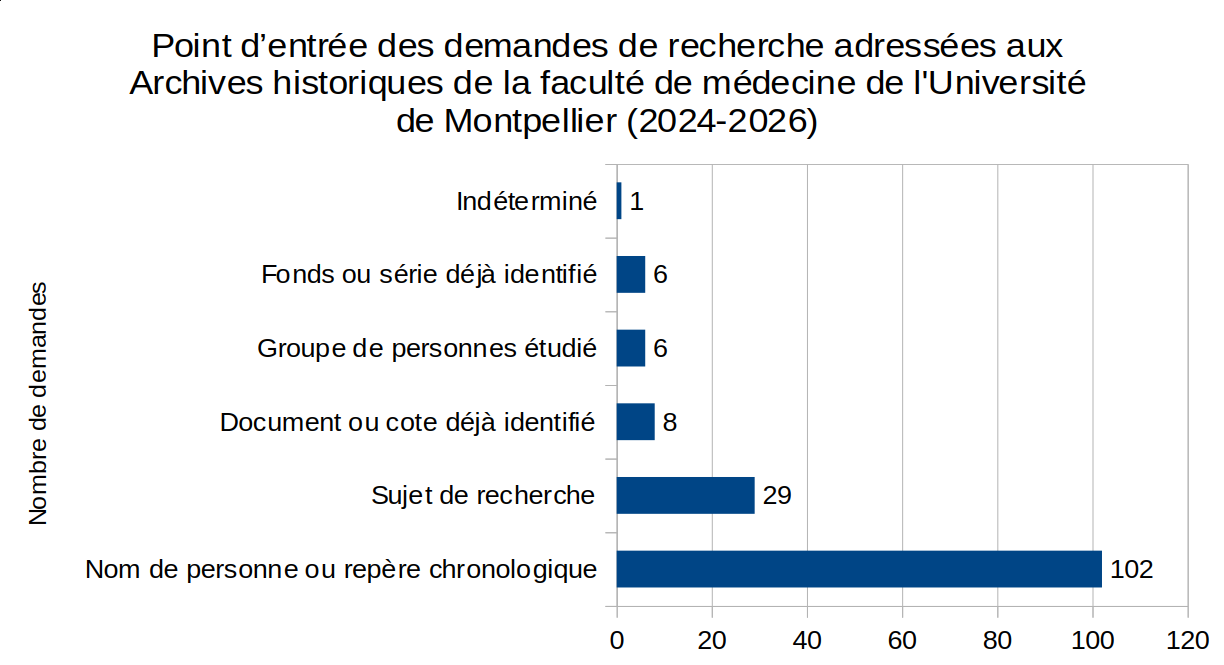
\includegraphics[width=0.88\textwidth]{images/point_entree_demandes_2024-2026.png}
	\caption[Point d'entrée des demandes de recherche, 2024--2026]
	{Point d'entrée des demandes de recherche adressées aux Archives historiques de la Faculté de médecine de l'Université de Montpellier entre 2024 et la pause estivale de la mi-juillet 2026. Graphique réalisé par Clara Martin à partir des données du suivi des demandes renseignées par la Mission Archives historiques.}
	\label{fig:point-entree-demandes}
\end{figure}

Ces chiffres renseignent moins sur la précision des demandes que sur la connaissance de l'organisation documentaire. Une recherche peut être clairement définie --- retrouver le parcours d'une personne à une date donnée, par exemple --- sans que son auteur sache dans quelle série ou sous quelle cote se trouve l'information. Le phénomène est particulièrement net pour la scolarité et les parcours universitaires : 103 demandes relèvent de cet objet, dont 86 prennent pour point d'entrée un nom de personne ou un repère chronologique. L'identification des registres, dossiers d'étudiants ou autres archives administratives pertinents repose alors sur le service.

Les consultations sur place présentent un profil différent. Comme pour les demandes par correspondance, chaque séance a été rattachée à un objet principal, déterminé d'après l'information recherchée plutôt que d'après les fonds mobilisés. Sur 76 séances, 25 concernent la scolarité et les parcours universitaires, soit 32,9\,\% ; 17 les enseignements, les pratiques et les savoirs médicaux ; 14 le patrimoine, les bâtiments et les collections ; 10 la vie et la carrière d'une personne ; et huit le gouvernement et l'histoire institutionnelle. Une séance relève de la catégorie \enquote{autre} et une demeure indéterminée. Plusieurs ensembles pouvant être consultés au cours d'une même séance, ces 76 consultations représentent 110 occurrences de fonds.

\begin{figure}[htbp]
	\centering
	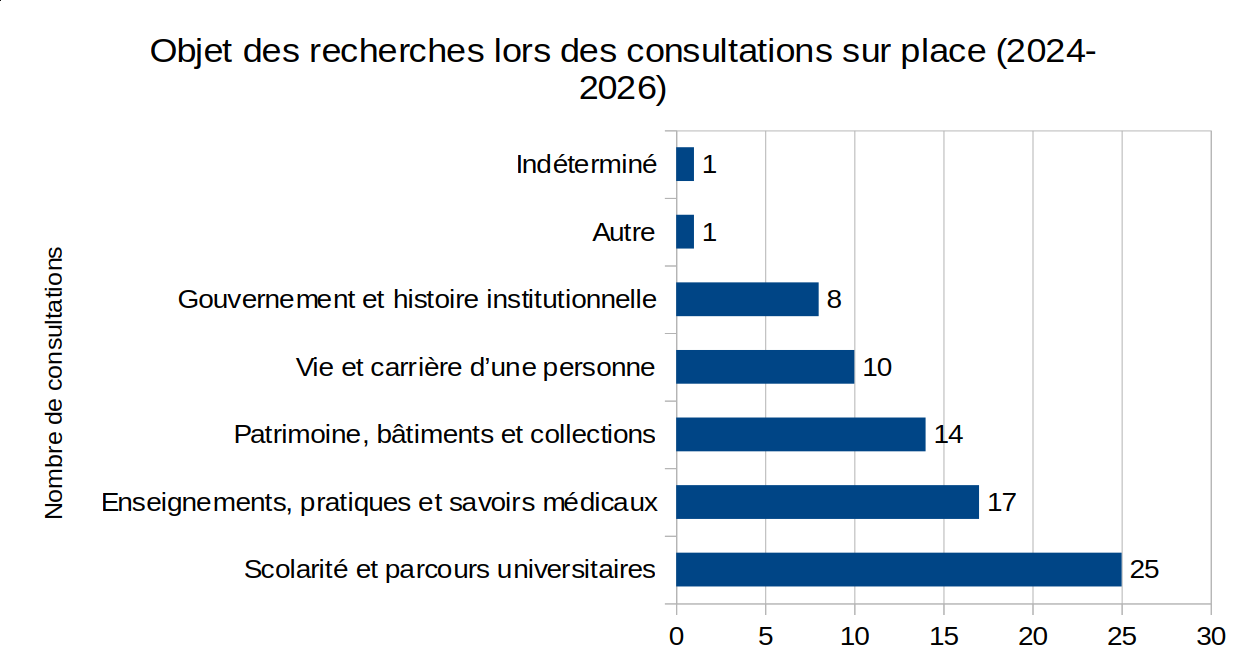
\includegraphics[width=0.88\textwidth]{images/objet_recherches_consultations_2024-2026.png}
	\caption[Objet des recherches lors des consultations sur place, 2024--2026]
	{Objet des recherches lors des consultations sur place entre 2024 et la pause estivale de la mi-juillet 2026. Graphique réalisé par Clara Martin à partir des données du suivi des consultations renseignées par la Mission Archives historiques.}
	\label{fig:objet-consultations}
\end{figure}

Cette différence tient en partie à la nature des recherches. Une demande familiale ou généalogique portant sur un parcours universitaire peut souvent être satisfaite par la vérification d'une mention et l'envoi de quelques reproductions ; une recherche universitaire ou érudite nécessite plus fréquemment la consultation suivie et croisée de plusieurs documents. La mise en ligne ne répond donc pas de la même manière à tous les usages : l'amélioration du \gls{signalement} peut bénéficier à l'ensemble des chercheurs, tandis que la numérisation présente un intérêt particulier pour les corpus faisant l'objet de demandes nominatives répétées.

Un premier besoin fonctionnel apparaît ainsi : permettre aux usagers de passer plus facilement de leur objet de recherche aux ensembles documentaires susceptibles d'y répondre, alors que cette identification repose encore largement sur la connaissance des fonds détenue par le personnel.

\paragraph{Une médiation documentaire qui représente une charge de travail mesurable}

Les 76 séances recensées entre 2024 et la pause estivale de la mi-juillet 2026 représentent 9\,955 minutes de consultation sur place, soit 165~h~55, auxquelles s'ajoutent 1\,150 minutes de préparation renseignées, soit 19~h~10. Le total documenté atteint ainsi 11\,105 minutes, soit un peu plus de 185 heures.

\begin{table}[htbp]
	\centering
	\small
	\caption{Temps mobilisé par les consultations sur place}
	\label{tab:temps-consultations}
	\begin{tabular}{lrrrr}
		\toprule
		\textbf{Année} &
		\textbf{Séances} &
		\textbf{Consultation (min)} &
		\textbf{Préparation (min)} &
		\textbf{Total (min)} \\
		\midrule
		2024 & 35 & 4\,575 & 55  & 4\,630 \\
		2025 & 23 & 3\,025 & 755 & 3\,780 \\
		2026 & 18 & 2\,355 & 340 & 2\,695 \\
		\midrule
		\textbf{Total} & \textbf{76} & \textbf{9\,955} & \textbf{1\,150} & \textbf{11\,105} \\
		\bottomrule
	\end{tabular}
	
	\vspace{0.3em}
	\begin{minipage}{0.93\textwidth}
		\footnotesize
		\emph{Source :} tableau élaboré par Clara Martin à partir des données du suivi des consultations renseignées par la Mission Archives historiques. Le temps de préparation n'était pas systématiquement indiqué, notamment en 2024 ; les valeurs présentées constituent donc un minimum. Les données de 2026 sont arrêtées à la pause estivale de la mi-juillet.
	\end{minipage}
\end{table}

Les 152 demandes traitées par correspondance représentent en outre 4\,485 minutes de travail renseigné, soit 74~h~45. Ce relevé demeure lui aussi partiel : le temps consacré à cinq demandes n'a pas été renseigné et les données de 2026 s'arrêtent à la mi-juillet. Ces chiffres ne permettent pas d'estimer directement le temps que ferait économiser une amélioration de l'accès en ligne, mais montrent qu'une part mesurable de l'activité est consacrée à identifier les sources, à préparer leur communication et à répondre individuellement aux demandes.

Pour 2025 et la période étudiée de 2026, 197 numérisations sont explicitement comptabilisées dans 32 envois dont le nombre d'images est renseigné ; 193 d'entre elles répondent à des demandes externes. La reproduction constitue donc déjà un mode courant de communication à distance. Pour certaines recherches nominatives, notamment relatives à la scolarité, la réponse consiste à repérer une mention dans un registre puis à en transmettre la reproduction. La mise en ligne des registres les plus sollicités pourrait éviter une partie de ces opérations répétées ; le même raisonnement vaut, dans une moindre mesure, pour certains registres anciens régulièrement demandés.

La publication des instruments de recherche répond à un besoin différent. Elle ne supprimera ni les demandes ni la médiation archivistique, mais elle peut permettre aux chercheurs d'effectuer eux-mêmes un premier repérage et d'adresser des demandes mieux documentées. Une meilleure visibilité peut parallèlement susciter de nouvelles recherches et consultations : l'objectif n'est donc pas simplement de réduire la charge de travail, mais d'éviter que le service assume systématiquement des opérations élémentaires pouvant être effectuées par l'usager, afin de concentrer sa médiation sur les recherches nécessitant réellement sa connaissance des fonds.

Deux besoins complémentaires se dégagent ainsi : signaler les fonds et les unités documentaires pertinents, puis donner sélectivement accès aux reproductions des corpus les plus sollicités.

\chapter{Structuration, publication et signalement des descriptions archivistiques}
\chapitrecourt{Signalement des descriptions archivistiques}

\section{Le mini-site institutionnel comme espace de médiation et de valorisation}

La création d'un mini-site institutionnel répond à un besoin distinct de ceux auxquels doivent satisfaire les outils de description et de diffusion examinés dans la suite de ce chapitre. Sans constituer une nouvelle base documentaire ni accueillir la production des instruments de recherche, il doit organiser l'accès aux fonds, aux instruments publiés, aux informations pratiques, aux contenus de valorisation et, le cas échéant, aux reproductions diffusées dans d'autres environnements.

Cette fonction a été éprouvée pendant le stage par un premier prototype développé localement en HTML, CSS et JavaScript, puis par sa transposition dans un environnement WordPress de préproduction de l'Université\footnote{Le contenu du prototype, ses choix éditoriaux, ses limites, son code source et sa version consultable sont présentés en annexe~\ref{annexe:prototype-mini-site}.}. Le premier permettait d'expérimenter librement l'organisation des contenus et les parcours de navigation ; le second confrontait ces choix aux conditions institutionnelles de publication. Le prototypage visait ainsi moins à préfigurer techniquement le site définitif qu'à déterminer les fonctions susceptibles d'être confiées à cette interface éditoriale.

\subsection{Expérimenter plusieurs parcours d'accès aux fonds}

Le prototype distingue quatre entrées principales --- l'accueil, les fonds et instruments de recherche, les expositions et la consultation --- auxquelles s'ajoute une restitution numérique du \enquote{musée des archives}. Elles correspondent à des intentions différentes : découvrir le service et ses fonds, identifier des documents, préparer leur consultation ou parcourir les archives à partir d'un récit ou d'une sélection patrimoniale.

Une interface consacrée à des collections ne peut présupposer que ses utilisateurs connaissent déjà la ressource recherchée. Si la requête répond efficacement à un besoin défini, elle rend moins perceptibles l'étendue et la diversité d'un ensemble documentaire ; des interfaces donnant davantage à voir les collections favorisent au contraire l'exploration, la découverte et le passage d'une vue générale à des ressources particulières\footcite{Whitelaw2015GenerousInterfaces}. Cette complémentarité correspond à la diversité des usages envisageables pour les archives historiques, depuis la recherche d'une cote précise jusqu'à une première découverte des fonds.

La rubrique documentaire donne donc une vue d'ensemble des fonds avant de conduire, lorsqu'ils existent, vers leurs instruments. Pour chaque instrument disponible sont indiqués sa cote, son intitulé, une courte description et un lien vers le PDF ou la ressource diffusée dans un autre environnement. Seuls les trois instruments déjà publiés en ligne --- les répertoires 1MED, 2MED et 1FiMED --- ont été intégrés ; les autres ensembles restent signalés sans donner accès à leurs instruments internes ou non publiés. Lors de la transposition du prototype local dans WordPress, la page qui réunissait initialement les fonds publics modernes et contemporains et les fonds privés a ainsi été répartie entre trois ensembles --- fonds ancien, fonds modernes et contemporains publics, et fonds privés --- afin d'en rendre l'organisation plus lisible.

Cette organisation privilégie un espace spécifiquement consacré aux archives plutôt que la dispersion de pages dans les rubriques thématiques du site institutionnel. Si cette dernière solution rapproche les activités passées et présentes, elle tend à privilégier les ensembles qui s'y prêtent le mieux ; un espace dédié permet de représenter plus largement les fonds communicables\footcite[pp.~94--95]{FerradouFine2011}.

Les plans de classement, encore en cours d'élaboration au moment du mémoire, n'ont pas été intégrés. À terme, une arborescence pourrait rendre visibles tous les ensembles conservés, y compris ceux dépourvus d'instrument publié, tandis que des notices synthétiques préciseraient leur contenu général, leurs dates extrêmes et leur état de traitement. Lorsqu'un instrument est disponible, un lien conduirait à sa présentation détaillée. La rubrique remplirait ainsi une fonction d'état général des fonds tout en distinguant leur existence, leur traitement archivistique et la publication de leurs instruments.

\subsection{Accompagner l'utilisateur vers les instruments de recherche}

Rendre les fonds visibles ne suffit pas à rendre leur organisation intelligible. Les instruments de recherche préservent la provenance, la hiérarchie et le contexte documentaire selon des principes et un vocabulaire qui ne correspondent pas nécessairement aux catégories à partir desquelles un utilisateur formule sa recherche. La description à plusieurs niveaux et des termes tels que \enquote{instrument de recherche}, \enquote{état des fonds} ou \enquote{cadre de classement} peuvent ainsi constituer des obstacles\footcite[pp.~25--26]{Homer2021}.

La diffusion sur le web accentue cette difficulté en éloignant l'instrument du contexte dans lequel sa consultation pouvait être accompagnée par un archiviste. La conformité aux standards descriptifs reste nécessaire, mais ne garantit pas à elle seule l'usage d'un instrument en ligne : terminologie, représentation de la hiérarchie, fonctions de recherche et présentation de l'information interviennent également\footcite[pp.~24--27]{AlfierFeliciati2017}. Des tests menés auprès d'utilisateurs montrent notamment les difficultés provoquées par des intitulés ambigus, des relations de navigation insuffisamment explicites, le jargon professionnel ou des hiérarchies dans lesquelles il devient difficile de se situer\footcite[pp.~30--35]{Walton2017FindingAids}.

Le mini-site ajoute donc un niveau d'explication sans modifier la structure scientifique des instruments. Une rubrique d'aide a été conçue pour expliquer l'organisation en fonds, le rôle de la cote ainsi que la localisation et la lecture des inventaires. Des formulations comme \enquote{fonds et collections} ou \enquote{recherche dans les inventaires} peuvent être plus accessibles que \enquote{cadre de classement}, tandis que les \enquote{archives numérisées} doivent être distinguées des autres ressources proposées en ligne\footcite[p.~28]{Homer2021}. Le vocabulaire archivistique n'est pas supprimé, mais introduit au moment où il devient nécessaire au parcours.

La mise en ligne d'un instrument ne garantit d'ailleurs pas son utilisation. Dans une enquête menée auprès des internautes des Archives départementales du Var, 95\,\% des répondants déclaraient consulter les documents numérisés, contre seulement 20\,\% les instruments de recherche, dont l'offre en ligne restait alors partielle\footcite[p.~154]{BugatDroguetJegouzo2007}. Sans transposer ces proportions au cas montpelliérain, cet écart distingue nettement disponibilité documentaire et appropriation des outils de repérage. Les Archives départementales de la Vendée proposaient ainsi un accès thématique destiné aux non-initiés parallèlement à un état des fonds davantage conçu pour les chercheurs familiers de l'organisation archivistique, complétés par des fiches méthodologiques guidant les recherches à partir d'objets concrets\footcite[p.~141]{Roy2012}.

La page consacrée à la consultation prolonge cette médiation jusqu'à l'accès physique aux documents. Elle rassemble les conditions d'accès, les coordonnées de la Mission et les informations utiles à une demande --- sujet de recherche, fonds ou cote éventuellement repérés, dates ou personnes concernées --- et explique comment identifier une cote et parcourir un inventaire. Liens internes, renvois vers les instruments et modalités de contact clairement indiquées doivent assurer la circulation entre ces différents niveaux d'information\footcite[p.~96]{FerradouFine2011}. Le mini-site prépare ainsi la recherche sans prétendre remplacer l'accompagnement archivistique lorsqu'il reste nécessaire.

Les documents rencontrés au cours de ces parcours doivent enfin demeurer reliés aux descriptions qui les contextualisent. Dans le cas des Arts Décoratifs, numérisation, documentation et indexation forment une même chaîne, tandis que thésaurus et mots-clés constituent des \enquote{passerelles} entre professionnels, amateurs et chercheurs\footcite[pp.~222--223]{Collin2017}. Pour les archives historiques, cette articulation conduit à permettre le passage entre document, fonds et instrument plutôt qu'à isoler les ressources de médiation de leur contexte archivistique.

\subsection{Reconstituer le \enquote{musée des archives} : faire de l'histoire de la valorisation un objet de médiation}

Le prototype a également permis d'expérimenter une forme de valorisation qui ne préexistait pas sous forme numérique. La rubrique consacrée aux expositions donne accès à l'exposition virtuelle \enquote{14--18, Médecine au champ d'honneur}\footcite{UMExpositionMedecine1418} ainsi qu'à la présentation et au livret numériques de l'exposition \enquote{Les Bâtisseurs de la Faculté de médecine du XX\textsuperscript{e} siècle}\footcite{BatisseursFaculte2021}\footcite{BatisseursFaculte2021Livret}. À ces ressources existantes s'ajoute une proposition conçue pendant le stage : la reconstitution numérique du \enquote{musée des archives} constitué par Joseph Calmette au début du XX\textsuperscript{e} siècle.

Après l'achèvement du classement du fonds ancien en 1908, Calmette avait disposé dans une vitrine du Musée Atger une sélection de pièces remarquables, dont il publia la liste dans le second tome du \emph{Cartulaire de l'Université de Montpellier}. Ces spécimens devaient donner un aperçu de la variété et de l'intérêt des archives et éveiller la curiosité des visiteurs pour l'histoire de la Faculté\footcite[p.~XVI--XXI, vues~35 à 40 de la version numérisée]{CalmetteCartulaire1912}. Aujourd'hui disparue, cette vitrine appartient elle-même à l'histoire de la patrimonialisation du fonds : le reclassement des archives anciennes s'accompagnait de leur exposition comme objets historiques.

La reconstitution reprend les vingt-deux pièces de cette sélection, chacune associée à sa cote, sa date, une courte présentation et une reproduction ; l'interface permet de parcourir l'ensemble ou d'accéder directement à une pièce et d'en agrandir l'image\footnote{Les reproductions ont été réalisées par Clara Martin au cours du stage. Certains documents, notamment des parchemins de la série B, ont été numérisés dans leur état matériel actuel et apparaissent donc encore pliés. Leur mise à plat et leur restauration doivent être effectuées ultérieurement par les ateliers du \gls{scdi}.}. Il ne s'agit donc ni de constituer une nouvelle sélection de \enquote{trésors} ni d'en faire un instrument de recherche autonome, mais de prendre pour objet un choix historique déjà constitué.

Le passage de la vitrine au dispositif numérique en transforme cependant les modalités d'exploration. Les pièces deviennent individuellement accessibles, tandis que leur cote et leur contextualisation permettent de revenir de l'objet remarquable vers l'ensemble archivistique auquel il appartient. Cette circulation entre vue d'ensemble, exploration et détail correspond aux possibilités d'interfaces patrimoniales qui ne réduisent pas l'accès aux collections à la formulation préalable d'une requête\footcite{Whitelaw2015GenerousInterfaces}. La reconstitution conserve ainsi le principe de la sélection de Calmette sans chercher à reproduire matériellement sa vitrine.

Elle rend simultanément accessibles les documents choisis et le geste qui les avait réunis. La liste publiée par Calmette devient la source permettant de restituer une manière historiquement située de présenter les archives de la Faculté. L'histoire du traitement et de la valorisation du fonds, étudiée dans la première partie, fournit ainsi elle-même la matière d'une expérimentation numérique contemporaine.

Pour les futurs contenus éditoriaux, le choix des pièces répondrait à d'autres critères. Les fonds retenus pour une valorisation institutionnelle doivent notamment être communicables, représentatifs de l'activité de l'établissement, liés aux thématiques traitées, suffisamment décrits et dotés d'un potentiel iconographique ; les documents les plus attractifs peuvent alors conduire vers des ensembles visuellement plus sobres mais plus riches sur le plan scientifique\footcite[pp.~92--94]{FerradouFine2011}. La valorisation repose ainsi sur une \enquote{mise en perspective et en contexte porteuse de sens}, tandis que le choix de l'outil doit découler du discours et des documents à présenter\footcite[pp.~363--366]{GueitMontchal2019}. La reconstitution du \enquote{musée des archives} en fournit ici une application : sa forme découle de l'objet historique qu'elle cherche à restituer.

\begin{figure}[htbp]
	\centering
	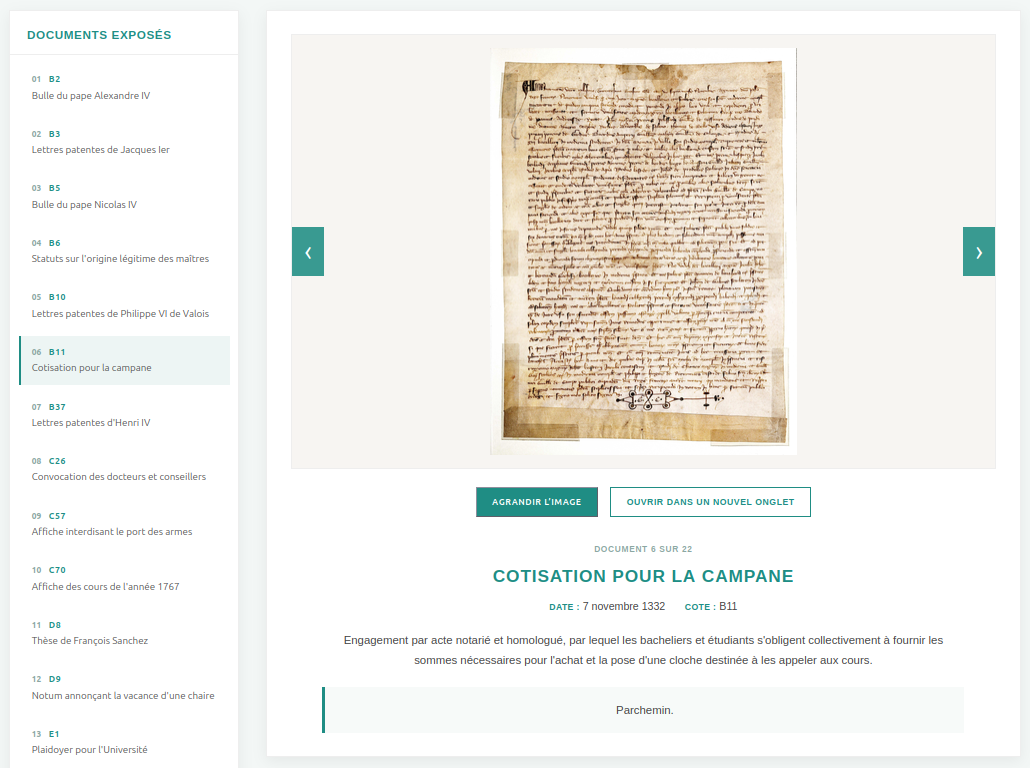
\includegraphics[width=\textwidth]{images/musee_des_archives.png}
	\caption{Prototype de restitution numérique du \enquote{musée des archives} de Joseph Calmette : navigation dans la sélection et contextualisation d'une pièce}
	\label{fig:prototype-musee-archives}
\end{figure}

\subsection{Inscrire la médiation dans l'environnement institutionnel}

La transposition du prototype dans l'environnement de préproduction de l'Université permettait enfin d'éprouver sa viabilité institutionnelle. Le site principal et plusieurs mini-sites de l'Université de Montpellier reposent sur WordPress, un \gls{cms} dont le cadre graphique, fonctionnel et éditorial impose davantage de contraintes que le prototype local.

Cette intégration évite de faire dépendre durablement la diffusion des Archives historiques d'un site autonome développé pendant le stage. L'Université assure l'hébergement, la maintenance, la sécurité et les mises à jour techniques, tandis que la Mission conserve la gestion scientifique et éditoriale de ses contenus. Cette répartition rejoint un modèle de publication dans lequel les détenteurs de l'information assurent son édition initiale au sein d'un dispositif commun de validation et de publication, plutôt qu'un fonctionnement centralisé autour d'un webmestre multipliant transmissions et rééditions\footcite[pp.~122--124]{Reymond2008Webometrie}. La Mission conserve ainsi la maîtrise de ses contenus archivistiques, tandis que la \gls{dsin} encadre leur publication technique.

Cette articulation suppose une coordination entre compétences archivistiques, éditoriales et techniques. À l'agence de l'eau Adour-Garonne, l'intégration des archives au site institutionnel avait ainsi associé le service des archives, les responsables éditoriaux et techniques et des usagers internes pour déterminer la place des pages dans l'arborescence, leur articulation avec la ligne éditoriale et leur adaptation à la charte graphique\footcite[pp.~92--96]{FerradouFine2011}. Le passage du prototype local à WordPress confronte de même les besoins définis par la Mission aux règles éditoriales de l'Université et aux possibilités techniques de la \gls{dsin}.

Cette inscription donne parallèlement aux archives une place identifiable dans la communication générale de l'établissement : elle permet de toucher ses publics, de moderniser leur image auprès du personnel, de légitimer leur place dans son patrimoine intellectuel et, par une meilleure identification des fonds et de leurs conditions d'accès, de contribuer à sa transparence\footcite[pp.~90--91 et 98--103]{FerradouFine2011}.

Le cadre institutionnel fixe toutefois les limites du mini-site. L'ajout de composants et les modifications techniques demeurent encadrés, tandis que l'affichage standard de WordPress ne répond pas aux besoins de consultation précise des manuscrits, parchemins, registres ou documents de grand format. Les échanges avec la \gls{dsin} et le service de la communication ont montré que des développements spécifiques, notamment l'intégration d'une visionneuse, restaient envisageables.\footnote{Les solutions permettant d'articuler descriptions archivistiques et reproductions numériques sont examinées au chapitre~\ref{chap:articulation-descriptions-reproductions}.} Le stockage et la diffusion des reproductions relèvent cependant d'autres dispositifs, de même que la production et la maintenance des instruments de recherche, qui doivent pouvoir être structurés, corrigés et actualisés sans ressaisie dans WordPress.

Une logique de \enquote{dissémination} peut précisément associer un site institutionnel consacré à l'orientation et à la médiation à des dispositifs distincts pour l'accès aux collections numérisées\footcite[p.~156]{Halais2012}. Le prototype permet ainsi de circonscrire la fonction du mini-site dans l'architecture de diffusion : rendre les fonds visibles, expliquer leur organisation, accompagner l'accès aux instruments, proposer des parcours de valorisation et orienter vers les ressources diffusées ailleurs. La production, la structuration et le \gls{signalement} des instruments relèvent dès lors d'outils spécialisés, qu'il convient maintenant d'examiner.

\section{La structuration et le signalement des instruments de recherche en EAD}
\label{sec:structuration-signalement-ead}

\subsection{L'EAD, format commun de structuration et d'échange}
\label{subsec:ead-format-echange}

\paragraph{La structure de la description archivistique}

La \gls{ead}, ou Description archivistique encodée, est un standard conçu pour représenter les instruments de recherche archivistiques sous une forme structurée. Développée à partir des années 1990 à l'initiative de la Society of American Archivists, elle répond aux besoins d'échange apparus avec l'informatisation des services d'archives et la diffusion des descriptions sur le web\footcite[pp.~84--85]{Sibille2012}.

L'\gls{ead} repose sur le \gls{xml}, syntaxe générique permettant de hiérarchiser, de contrôler, d'interroger, de transformer et d'échanger des données. Elle lui associe un vocabulaire propre à la description archivistique : l'\gls{ead} 2002 prévoit notamment des éléments pour la cote (\texttt{<unitid>}), l'intitulé (\texttt{<unittitle>}), les dates (\texttt{<unitdate>}), le producteur (\texttt{<origination>}) ou la présentation du contenu (\texttt{<scopecontent>})\footcite{EAD2002Dictionnaire}. La fonction de chaque information devient ainsi explicite et exploitable indépendamment de sa mise en page.

Les composants emboîtés restituent l'organisation d'un fonds, de ses principales subdivisions jusqu'aux dossiers ou aux pièces. Ils permettent de mettre en œuvre les quatre principes de la description à plusieurs niveaux formalisés par la norme \gls{isadg} : description du général au particulier, adaptation des informations au niveau décrit, mise en relation des niveaux et non-répétition des informations\footcite[pp.~12--13]{ISADG2000}. Les deux \glspl{referentiel} ne se confondent donc pas : \gls{isadg} définit les principes de la description, tandis que l'\gls{ead} fournit une structure informatique pour les encoder\footcite{EAD2002Dictionnaire}.

\paragraph{Un format d'échange et d'interopérabilité}

La séparation entre les données et leur restitution permet d'exploiter un même instrument dans plusieurs environnements : affichage dans une interface de consultation, transmission à un autre système, agrégation dans un catalogue collectif ou production de nouvelles restitutions. À la différence d'un fichier Word ou PDF, dont les informations restent liées à une présentation déterminée, l'\gls{ead} rend leurs composantes accessibles à des traitements automatisés\footnote{Il s'agit notamment de la validation par rapport à un schéma ou à une \gls{dtd}, de l'interrogation et de l'extraction ciblées, de l'indexation par un moteur de recherche, de la transformation au moyen de feuilles de style XSLT ou de la conversion vers d'autres formats à partir d'une même source \gls{xml}.}.

La normalisation contribue ainsi à homogénéiser et à décloisonner les descriptions produites par différentes institutions\footcite[pp.~121--122]{Motte2015}. Elle ne suffit toutefois pas à garantir leur \gls{interoperabilite} : des standards peuvent décrire des objets distincts selon des granularités différentes, de sorte que leur articulation exige une analyse des modèles et la définition de correspondances explicites\footcite{MirandaEtAl2025}.

Pour les Archives historiques de la Faculté de médecine, l'\gls{ead} fournit un cadre commun pour reprendre des instruments aujourd'hui conservés sous forme de fichiers Word, PDF ou de tableaux. Il permet surtout de dissocier les descriptions de leur interface de publication, afin de les corriger et de les réutiliser dans plusieurs dispositifs sans les ressaisir.

L'\gls{ead} 2002 demeure la version employée à la BnF et dans la très grande majorité des institutions françaises\footcite{BnFEADGeneralites}. Cette persistance coexiste avec l'évolution internationale du standard : l'\gls{ead}~4 a été officiellement lancé le 31 juillet 2026\footcite{EAD4Release2026}. Les expérimentations conduites pendant le stage ont néanmoins porté sur l'\gls{ead} 2002, qui correspond aux chaînes de traitement étudiées.

\paragraph{La préparation de la rétroconversion}

La \gls{retroconversion} ne consiste pas à remplacer mécaniquement des éléments de mise en page par des balises. Elle suppose d'identifier la fonction archivistique des informations et de reconstruire les relations parfois seulement matérialisées par des titres, des retraits ou des changements de style. Une même présentation peut recouvrir des fonctions différentes selon les instruments ; inversement, une relation hiérarchique peut être exprimée sans être explicitement désignée.

Les retours d'expérience recommandent donc d'identifier des familles d'instruments suffisamment régulières, puis de définir pour chacune un modèle cible et des règles de conversion documentées\footcite{GouletMaftei2006}\footcite{Meissner1997}. Les correspondances stables peuvent être automatisées, tandis que les ambiguïtés de structure, les variations de rédaction et les informations implicites nécessitent un contrôle archivistique.

Le chantier de dématérialisation des Archives nationales reposait ainsi sur des consignes établies pour chaque instrument et sur une chaîne distinguant numérisation, restitution du texte, encodage et saisie des cotes, avec un contrôle propre à chaque opération\footcite[pp.~199--202]{Aristide2010}. L'analyse conduite pendant le stage a suivi une logique comparable : repérage des structures récurrentes, détermination des informations normalisables, formalisation de règles de saisie et contrôle de la restitution des cotes et des niveaux. Ce travail préparatoire a permis d'évaluer plusieurs chaînes de production de fichiers en \gls{ead} adaptées aux moyens du service.

\subsection{L'identification institutionnelle, préalable au signalement}
\label{subsec:identification-institutionnelle}

La circulation des descriptions suppose d'identifier de manière univoque l'institution qui en assume la responsabilité. La \gls{isdiah} fait ainsi de l'identifiant un élément obligatoire de la description des institutions conservant des archives et prévoit l'enregistrement d'un code unique conforme aux normes nationales et internationales applicables\footcite[pp.~13 et 16]{ISDIAH2008}. La norme \gls{isadg} l'intègre à la référence des unités de description, composée notamment du code du pays, du code du service d'archives et de la cote locale\footcite{ISADG2000}.

En France, l'identifiant unique des services d'archives est attribué par le \gls{siaf}, seul habilité à le délivrer\footcite[p.~4]{SIAFEnquete2025}. Il intervient également dans la construction de l'identifiant unique des entrées\footcite{SchemaRegistreEntrees}.

La position institutionnelle particulière de la Mission Archives historiques ne permet pas de déterminer directement le code sous lequel signaler ses fonds.\footnote{Cette position institutionnelle est exposée au chapitre~\ref{chap:cadre-juridique-derogation}.} La consultation du \gls{siaf} doit donc établir si les descriptions peuvent être rattachées à un identifiant existant ou si un identifiant propre doit être attribué. Cette clarification n'empêche pas leur structuration en \gls{ead}, mais conditionne leur versement effectif dans FranceArchives.

\subsection{SimplEAD : une chaîne légère de rétroconversion vers FranceArchives}
\label{subsec:simplead-francearchives}

\paragraph{Le signalement dans FranceArchives}

Mis en ligne en 2017 par le Service interministériel des Archives de France (\gls{siaf}), FranceArchives agrège et rend interrogeables dans un moteur fédéré les instruments de recherche d'institutions et de services publics ou privés, produits dans des environnements techniques hétérogènes\footcite[pp.~34--35]{Restif2021}. Le portail offre ainsi un point d'accès commun à leurs descriptions sans se substituer aux institutions de conservation ni à leurs propres interfaces. Il n'héberge pas les images numérisées, mais peut renvoyer vers les reproductions consultables sur les sites sources\footcite{FranceArchivesContenu}\footcite{FranceArchivesRejoindre2026}. Pour les Archives historiques, ce référencement national compléterait donc la diffusion assurée par l'Université.

En 2021, environ 80\,\% des instruments intégrés étaient encodés en \gls{ead} ; des fichiers PDF ou CSV accompagnés de \glspl{metadonnees} en Dublin Core pouvaient également être reçus\footcite[p.~36]{Restif2021}. L'alimentation s'effectue par transmission de fichiers ou, lorsque le contributeur dispose de l'infrastructure nécessaire, par récupération automatisée de ses données\footcite{FranceArchivesRejoindre2026}. SimplEAD répond au cas des services qui ne produisent pas directement de fichiers en \gls{ead}.

\paragraph{L'organisation du modèle d'import}

SimplEAD convertit en \gls{xml}-\gls{ead} 2002 un instrument préparé dans un modèle tabulaire disponible aux formats Excel (\texttt{.xlsx}) et OpenDocument (\texttt{.ods})\footcite{FranceArchivesSimplEAD}. Les données sont saisies localement, puis le fichier est chargé dans le convertisseur, qui génère le document \gls{ead} sans exiger la rédaction directe du code \gls{xml} ni le déploiement d'un système d'information archivistique.

La chaîne a été expérimentée sur quatre instruments présentant des structures différentes : les archives relatives aux legs Bouisson-Bertrand et Jaumes (\texttt{LEG}), celles de la maïeutique (\texttt{MAIE}), le fonds d'affiches de la Faculté (\texttt{1 Fi/MED}) et le sous-fonds consacré à la transfusion sanguine d'Émile Jeanbrau (\texttt{1EJ}). Le périmètre de FranceArchives incluant les descriptions produites par des institutions privées, la nature juridique de certains de ces fonds ne constitue pas un obstacle à leur \gls{signalement}\footcite[p.~35]{Restif2021}.

Le modèle d'import fourni par SimplEAD comporte trois feuilles, dont les fonctions et les correspondances avec l'\gls{ead} sont distinctes\footcite{FranceArchivesSimplEADDocumentation}.

\begin{table}[htbp]
	\centering
	\scriptsize
	\setlength{\tabcolsep}{4pt}
	\renewcommand{\arraystretch}{1.15}
	\caption{Structure du modèle d'import SimplEAD utilisé pendant l'expérimentation}
	\label{tab:structure-simplead}
	
	\begin{tabularx}{\textwidth}{
			>{\raggedright\arraybackslash}p{2.7cm}
			>{\raggedright\arraybackslash}p{3.1cm}
			>{\raggedright\arraybackslash}X
		}
		\toprule
		\textbf{Feuille} &
		\textbf{Fonction} &
		\textbf{Champs} \\
		\midrule
		
		\texttt{intitulé\_inventaire} &
		Identification et responsabilité de l'instrument ; identification du producteur &
		Identifiant de l'inventaire ; titre ; sous-titre ; responsable de la conservation ; adresse ; date de publication ; auteur ; producteur ; type de producteur. \\
		
		\addlinespace
		
		\texttt{description\_du\_fonds} &
		Description de haut niveau correspondant principalement à \texttt{archdesc} &
		Titre ; dates de début et de fin ; description physique ; cote ; description du contenu ; indexation par lieu, personne, institution et matière ; conditions d'accès ; niveau de description de l'inventaire ; langue ; conditions d'utilisation et de reproduction ; modalité d'entrée. \\
		
		\addlinespace
		
		\texttt{description\_cotes} &
		Description hiérarchisée des unités documentaires au moyen de composants \texttt{<c>} &
		Niveau ; titre ; cote ; dates de début et de fin ; description physique ; description du contenu ; indexation par lieu, personne, institution et matière ; conditions d'accès ; profondeur de la description archivistique. \\
		
		\bottomrule
	\end{tabularx}
	
	\vspace{0.3em}
	
	\begin{minipage}{0.95\textwidth}
		\footnotesize
		\emph{Source :} modèle d'import SimplEAD utilisé dans le cadre du stage et documentation du Service interministériel des Archives de France.
	\end{minipage}
\end{table}

La première feuille ne correspond pas intégralement à un seul bloc de l'\gls{ead}. Les informations éditoriales alimentent notamment \texttt{eadheader}, tandis que les champs \enquote{Producteur} et \enquote{Type de producteur} sont convertis en \texttt{origination} et en \texttt{persname} ou \texttt{corpname}. L'identifiant de l'instrument doit être unique, pérenne et préfixé par le code du service contributeur.\footnote{La détermination de ce code est examinée à la sous-section~\ref{subsec:identification-institutionnelle}.} Le sous-titre n'étant exploité ni par FranceArchives ni par le portail européen des archives, il ne doit pas contenir une information indispensable au repérage de l'instrument\footcite{FranceArchivesSimplEADDocumentation}.

Plusieurs valeurs d'indexation de même nature sont séparées par une arobase, tandis que des listes déroulantes contrôlent certains champs afin de limiter les variantes de saisie\footcite{FranceArchivesSimplEAD}\footcite{FranceArchivesSimplEADDocumentation}. La qualité du \gls{signalement} dépend néanmoins de la normalisation des points d'accès. La documentation recommande l'emploi des formes d'autorité proposées par FranceArchives, l'hétérogénéité de la description et de l'indexation constituant l'une des principales difficultés d'exploitation des données agrégées\footcite{FranceArchivesSimplEADDocumentation}\footcite[p.~40]{Restif2021}.

\paragraph{La restitution de la hiérarchie}

SimplEAD distingue la position d'une unité dans l'arborescence de son niveau archivistique. La colonne \enquote{Niveau} attribue à chaque ligne un rang compris entre 1 et 5 et commande l'emboîtement des composants. La colonne \enquote{Profondeur de la description archivistique} qualifie l'unité décrite et alimente l'attribut \texttt{@level} de l'élément \texttt{<c>}\footcite{FranceArchivesSimplEADDocumentation}. Sa liste contrôlée comprend notamment \enquote{groupe de documents}, \enquote{sous-groupe de documents}, \enquote{série organique}, \enquote{sous-série organique}, \enquote{dossier}, \enquote{pièce} et \enquote{autre niveau de description}.

Ces informations sont indépendantes : une unité placée au cinquième rang peut décrire un dossier, tandis qu'un dossier peut apparaître au deuxième rang dans une arborescence moins développée. De même, une rubrique ne doit être qualifiée de \enquote{série organique} que si elle correspond à un ensemble constitué par l'activité du producteur ; lorsqu'elle résulte du classement, \enquote{groupe de documents} ou \enquote{sous-groupe de documents} constitue une qualification plus appropriée.

L'instrument \texttt{MAIE} a permis de tester les cinq rangs disponibles. La branche consacrée aux inscriptions enchaîne \enquote{Gestion de l'enseignement} au niveau 1, \enquote{Organisation des études} au niveau 2, \enquote{Inscriptions} au niveau 3, \enquote{Fiches d'inscription} au niveau 4, puis les dossiers \texttt{MAIE55} et \texttt{MAIE56} au niveau 5. Les quatre premiers composants organisent intellectuellement les dossiers décrits au dernier niveau.

Le rattachement dépend de l'ordre des lignes. Une unité de niveau 5 relève du dernier niveau 4 qui la précède ; plusieurs lignes successives de niveau 5 constituent des unités sœurs. Le retour de 5 à 3 ferme les niveaux 5 et 4 avant d'ouvrir une nouvelle branche sous le dernier niveau 2 rencontré. De même, le passage de 4 à 1 clôt toute la branche précédente avant d'ouvrir un nouveau composant de premier niveau. Une remontée peut donc franchir plusieurs rangs sans ambiguïté ; en revanche, le passage de 3 à 5 laisserait l'unité de niveau 5 dépourvue de parent au niveau 4.

Le fichier généré doit enfin être contrôlé afin de vérifier que cette succession a été correctement traduite par l'emboîtement des composants \texttt{<c>}.

\paragraph{Une chaîne de publication, non un outil de gestion}

Les essais ont permis de générer les fichiers \gls{xml}-\gls{ead}, mais leur versement dans FranceArchives demeure subordonné à l'identification des Archives historiques comme service contributeur\footnote{Les modalités de cette identification sont exposées à la sous-section~\ref{subsec:identification-institutionnelle} et ses conséquences sur le choix de la chaîne sont reprises dans la conclusion du chapitre.}.

SimplEAD offre une solution proportionnée pour convertir et signaler des instruments stabilisés sans déployer immédiatement un système d'information archivistique. Il ne constitue toutefois ni un environnement de production partagée ni un outil de maintenance : les fichiers sources restent conservés localement et toute correction impose une nouvelle conversion, puis une nouvelle transmission.

Une alimentation automatisée repose sur une autre architecture. Le protocole \gls{oaipmh} permet à un fournisseur de données d'exposer sur le web des \glspl{metadonnees} structurées en \gls{xml}, qu'un fournisseur de services récupère au moyen de requêtes \gls{http}\footcite{OAIPMH2002}. FranceArchives peut ainsi actualiser les descriptions depuis le système du contributeur sans recevoir un nouveau fichier après chaque modification\footcite{FranceArchivesRejoindre2026}.

SimplEAD répond donc à la rétroconversion ponctuelle et au \gls{signalement} national d'instruments stabilisés. Leur gestion continue appelle en revanche un environnement partagé, dont Calames fournit un autre modèle.

\subsection{Calames : un environnement de production, de maintenance et de diffusion de l'EAD}
\label{subsec:calames}

Calames, Catalogue en ligne des archives et des manuscrits de l'enseignement supérieur, permet de produire et de maintenir directement les instruments en \gls{ead}, plutôt que de les préparer dans un format intermédiaire avant conversion.

\paragraph{Un catalogue collectif fondé sur la production directe en EAD}

Développé et administré par l'\Gls{abes}, Calames est un catalogue collectif consacré aux archives et manuscrits conservés dans les établissements français de l'enseignement supérieur et de la recherche\footcite{ABESCatalogueCalames}. Il est notamment issu de la \gls{retroconversion} du \textit{Catalogue général des manuscrits des bibliothèques publiques de France} (CGM), vaste entreprise de recensement et de description des manuscrits conservés dans les bibliothèques françaises, publiée en volumes à partir du XIX\textsuperscript{e} siècle. Calames a permis de reprendre ces descriptions dans un environnement où les établissements peuvent les corriger, les enrichir et les diffuser\footcite{Nicolas2007}. Il associe ainsi un catalogue public à une application professionnelle de production et de maintenance des instruments de recherche\footcite{Nicolas2008CalamesCatalogage}. Cette triple fonction d'outil d'encodage en \gls{ead}, d'interface publique et de réseau de production était déjà mise en évidence dans le bilan prospectif réalisé par l'\Gls{abes} en 2014\footcite{ABESCalamesBilan2014}.

La production s'effectue dans Calames Pro, qui repose sur XMetaL, un éditeur de documents \gls{xml} adapté par l'\Gls{abes} aux besoins du catalogage en \gls{ead}. Son interface masque une grande partie de la syntaxe \gls{xml} tout en laissant visible la structure hiérarchique : le catalogueur intervient sur les éléments de l'instrument sans saisir directement les balises\footcite{Nicolas2008CalamesCatalogage}. L'outil permet de créer et de modifier les différents niveaux de description, d'organiser les fichiers qui composent l'instrument et d'en contrôler la publication.

Contrairement à SimplEAD, où les données sont saisies dans un tableur avant leur conversion, l'instrument est directement créé et maintenu sous une forme structurée. Une correction ou un enrichissement peut ainsi être apporté sans nouvelle \gls{retroconversion}. Un fonds peut également recevoir une description synthétique, puis être détaillé à mesure de l'avancement du classement. Calames constitue donc à la fois un environnement de catalogage, une interface de diffusion et un réseau d'expertise\footcite{LatourCalames2021}.

\paragraph{La normalisation, l'indexation et les autorités}

La production dans Calames implique une normalisation et une indexation des données. La première applique des règles communes de description afin d'assurer l'homogénéité des instruments produits par les établissements du réseau ; la seconde associe aux unités décrites des points d'accès, notamment des noms de personnes, de collectivités, de lieux ou des sujets, afin de permettre leur recherche au-delà de la seule arborescence\footcite{ABESCatalogageCalames}.

Pour les personnes et les collectivités, Calames s'articule avec IdRef (\textit{Identifiants et Référentiels}), le \gls{referentiel} d'autorités de l'\Gls{abes}. Calames Pro permet ainsi d'associer aux points d'accès une forme normalisée et l'identifiant de l'autorité correspondante, dans le prolongement du contrôle d'autorité prévu dès sa conception à partir des données du Sudoc\footcite{AbesIdRef}\footcite{Nicolas2008CalamesCatalogage}. Cette fonction demeure largement mobilisée : environ 78\,000 nouveaux liens vers des autorités IdRef ont été publiés dans Calames en 2023\footcite{ABESStatistiquesCalames2023}\footnote{Les possibilités offertes par ces identifiants pour relier les personnes décrites dans les archives à d'autres ressources documentaires et scientifiques seront examinées dans la troisième partie (voir section~\ref{sec:idref})}.

\paragraph{Un environnement déjà implanté à l'Université de Montpellier}

Calames est déjà utilisé à l'Université de Montpellier. Les descriptions montpelliéraines sont réunies dans un ensemble intitulé \enquote{Manuscrits et archives des Universités de Montpellier}, qui comporte une branche consacrée à l'Université de Montpellier et une autre à l'Université Paul-Valéry Montpellier\footcite{CalamesArchivesUniversitesMontpellier}. La première comprend notamment les fonds de la Bibliothèque universitaire historique de médecine. Pascaline Todeschini, responsable des fonds patrimoniaux de cette bibliothèque, est par ailleurs référente Calames pour les deux universités montpelliéraines.

Les Archives historiques pourraient y former une branche distincte de celles des bibliothèques universitaires, plutôt que d'être rattachées aux collections de la Bibliothèque universitaire historique de médecine. Chaque établissement participant au réseau est identifié par un numéro \gls{rcr} Calames, attribué par l'\Gls{abes}. Dans Calames, cet identifiant couvre le périmètre institutionnel de l'établissement, indépendamment du nombre de bibliothèques ou de services qui y produisent des descriptions\footcite{ABESCatalogageCalames}.

Le \gls{rcr} est inscrit dans les fichiers \gls{ead} afin d'identifier l'établissement responsable de la conservation et de rattacher les descriptions à celui-ci dans le catalogue. Les fichiers produits dans Calames Pro sont également associés à des groupes d'utilisateurs qui déterminent les droits de modification. L'utilisation de XMetaL suppose enfin des accès professionnels et la disponibilité des licences nécessaires.

L'Université disposant déjà d'un \gls{rcr} Calames, l'enjeu n'est donc pas nécessairement d'en créer un nouveau, mais de déterminer avec la référente et l'\Gls{abes} dans quelles conditions les Archives historiques pourraient rejoindre le périmètre existant, disposer de droits de catalogage et être représentées comme une branche distincte. La question est ainsi autant institutionnelle que technique.

\begin{figure}[htbp]
	\centering
	
	\begin{forest}
		for tree={
			grow'=south,
			parent anchor=south,
			child anchor=north,
			align=center,
			edge={-},
			l sep=12pt,
			s sep=8pt,
			inner sep=3pt,
			font=\small,
		}
		[Manuscrits et archives\\des Universités de Montpellier
		[Université de Montpellier
		[Bibliothèque universitaire\\historique de médecine
		[Manuscrits]
		[Archives et\\fonds particuliers]
		]
		[\textit{Archives historiques}\\
		\textit{de la Faculté de médecine}\\
		\textit{(intégration envisagée)}]
		]
		[Université Paul-Valéry\\Montpellier
		[Ensembles documentaires\\propres à l'UMPV]
		]
		]
	\end{forest}
	
	\caption{Schéma simplifié de l'arborescence Calames des Universités de Montpellier et positionnement envisagé des Archives historiques}
	\label{fig:arborescence-calames}
\end{figure}

\paragraph{De la production locale à la diffusion nationale}

Les instruments maintenus dans Calames peuvent être publiés dans le catalogue collectif et leurs données réutilisées dans d'autres dispositifs\footcite{ABESReutilisationCalames}. Cette possibilité est inscrite dans la conception même de l'outil, qui permet notamment d'exporter les données vers d'autres environnements\footcite{Nicolas2008CalamesCatalogage}. FranceArchives et Calames remplissent ainsi des fonctions complémentaires : le premier agrège les descriptions de nombreux services d'archives, tandis que le second constitue un environnement de production et un catalogue spécialisé dans les archives et manuscrits de l'enseignement supérieur.

Calames dispose notamment d'un entrepôt \gls{oaipmh} qui expose ses \glspl{metadonnees} en vue de leur \gls{moissonnage} par d'autres systèmes\footcite{ABESOAICalames2017}. Un travail a été engagé entre l'\Gls{abes} et le \gls{siaf} afin d'améliorer l'exploitation de ce flux par FranceArchives\footcite{MichelNaddeo2023}. Pour les Archives historiques, l'objectif serait d'éviter la maintenance de versions indépendantes d'un même instrument dans le site de l'Université, Calames et FranceArchives. Les descriptions seraient maintenues dans Calames, puis réutilisées dans plusieurs interfaces, ce qui permettrait de mieux articuler des ressources aujourd'hui dispersées entre le site institutionnel, Foli@, WordPress et différents espaces internes.

\paragraph{Un outil de signalement, non un portail de valorisation}

Calames ne répond cependant pas à l'ensemble des besoins du projet. Son cœur fonctionnel demeure la production, l'indexation et la diffusion des instruments de recherche. La présentation du service, les expositions virtuelles et la mise en valeur éditoriale des collections relèvent davantage du site institutionnel.

L'hébergement des reproductions et leur consultation avancée au moyen de \gls{iiif} constituent également une fonction distincte.\footnote{L'articulation entre descriptions archivistiques et reproductions numériques est examinée au chapitre~\ref{chap:articulation-descriptions-reproductions}.} Le rapport prospectif consacré à Calames identifiait déjà l'articulation entre \gls{signalement} et numérisation parmi les enjeux d'évolution du catalogue\footcite{ABESCalamesBilan2014}. L'architecture envisagée peut donc être distribuée : Calames assurerait la production et la diffusion des instruments en \gls{ead}, le mini-site leur valorisation éditoriale et un service distinct l'hébergement et l'exposition interopérable des reproductions.

\paragraph{Une intégration suspendue à la refonte de Calames dans le cadre du projet Orion}

La possibilité d'une intégration dans Calames doit être replacée dans la transformation actuelle des outils de l'\Gls{abes}. Dans le cadre du projet Orion, qui prévoit notamment la refonte de Calames, les nouveaux déploiements dans le catalogue sont suspendus jusqu'en 2028 et les évolutions significatives des interfaces existantes sont gelées, bien que la continuité du service soit maintenue\footcite{FilAbesOrion2026}. Cette suspension intervient alors que le catalogue est déjà largement alimenté : fin 2023, sa base de production comptait plus de 1,7 million de composants \gls{ead}\footcite{ABESStatistiquesCalames2023}.

Orion porte plus largement sur le renouvellement du système de gestion des \glspl{metadonnees} du Sudoc et de ses services associés\footcite{AbesOrion2026}. Le marché a été attribué à Clarivate en mai 2026. La future infrastructure reposera notamment sur Alma, plateforme assurant la gestion unifiée des ressources physiques, électroniques et numériques ainsi que de leurs \glspl{metadonnees}\footcite{ExLibrisAlmaDocumentation}, et sur Primo, interface de découverte chargée d'indexer ces données et d'en permettre la recherche et la consultation\footcite{ExLibrisPrimoDocumentation}. Sa mise en production est prévue au plus tard au début de l'année 2028\footcite{FilAbesOrionClarivate2026}. Elle doit favoriser la circulation des données dans l'écosystème de l'enseignement supérieur et de la recherche en s'appuyant sur des protocoles standards, dont \gls{oaipmh}, ainsi que sur des \glspl{api}, interfaces permettant à des applications d'échanger automatiquement des données en lecture et en écriture\footcite{FilAbesOrionClarivate2026}.

La refonte de Calames s'inscrit donc dans le même programme de transformation, sans que ses modalités techniques puissent être déduites de celles déjà retenues pour le Sudoc. Alma et Primo concernent le renouvellement de ce dernier et de ses services associés, tandis que l'architecture du futur environnement de production et de diffusion des archives et manuscrits reste à préciser. La suspension actuelle de nouveaux déploiements dans Calames correspond précisément à cette période de transition.

Pour les Archives historiques de Montpellier, une incertitude supplémentaire demeure : l'Université étant déjà membre du réseau Calames, il reste à déterminer si leur intégration serait considérée comme un nouveau déploiement, actuellement suspendu, ou comme l'extension d'une structure existante. Calames ne peut donc pas être considéré comme une solution immédiatement opérationnelle pour la Mission, sans que son intérêt à moyen terme soit remis en cause.

\paragraph{Les limites de Calames au regard de la gestion archivistique}

Calames n'est enfin pas un \gls{sia} complet. Centré sur la description et le \gls{signalement}, il ne prend pas en charge la gestion des versements, des éliminations, des communications, des récolements, des localisations physiques ou du cycle de vie des documents. Cette limite est particulièrement sensible pour les archives scientifiques, dont le \gls{signalement} doit s'articuler avec un écosystème plus large de gestion et de conservation, notamment lorsqu'elles sont nativement numériques\footcite{MichelNaddeo2023}.

Ces besoins concernent également les archives courantes et intermédiaires de l'Université.\footnote{Ils sont examinés au chapitre~\ref{chap:systemes-information-archivistiques} consacré aux systèmes d'information archivistiques.} Calames et un éventuel \gls{sia} ne sont donc pas concurrents : le premier assure la description normalisée et le \gls{signalement} dans l'enseignement supérieur ; le second prend en charge les processus métier du service d'archives.

\section*{Conclusion du chapitre}
\phantomsection
\label{sec:conclusion-signalement}

Deux chaînes peuvent donc être engagées progressivement : SimplEAD pour rétroconvertir à court terme les instruments stabilisés vers FranceArchives, avec maintenance du fichier local, puis Calames ou son successeur comme environnement partagé de production, de maintenance et de diffusion, sous réserve de l'identification institutionnelle de la Mission, de ses conditions d'intégration au réseau et du calendrier de refonte. Le projet Orion renouvelle parallèlement l'infrastructure documentaire de l'\Gls{abes} sans permettre encore de préjuger de l'architecture du futur Calames. Dans les deux cas, production et \gls{signalement} des descriptions restent distincts de la médiation assurée par le mini-site.

\begin{landscape}
	\begin{figure}[p]
		\centering
		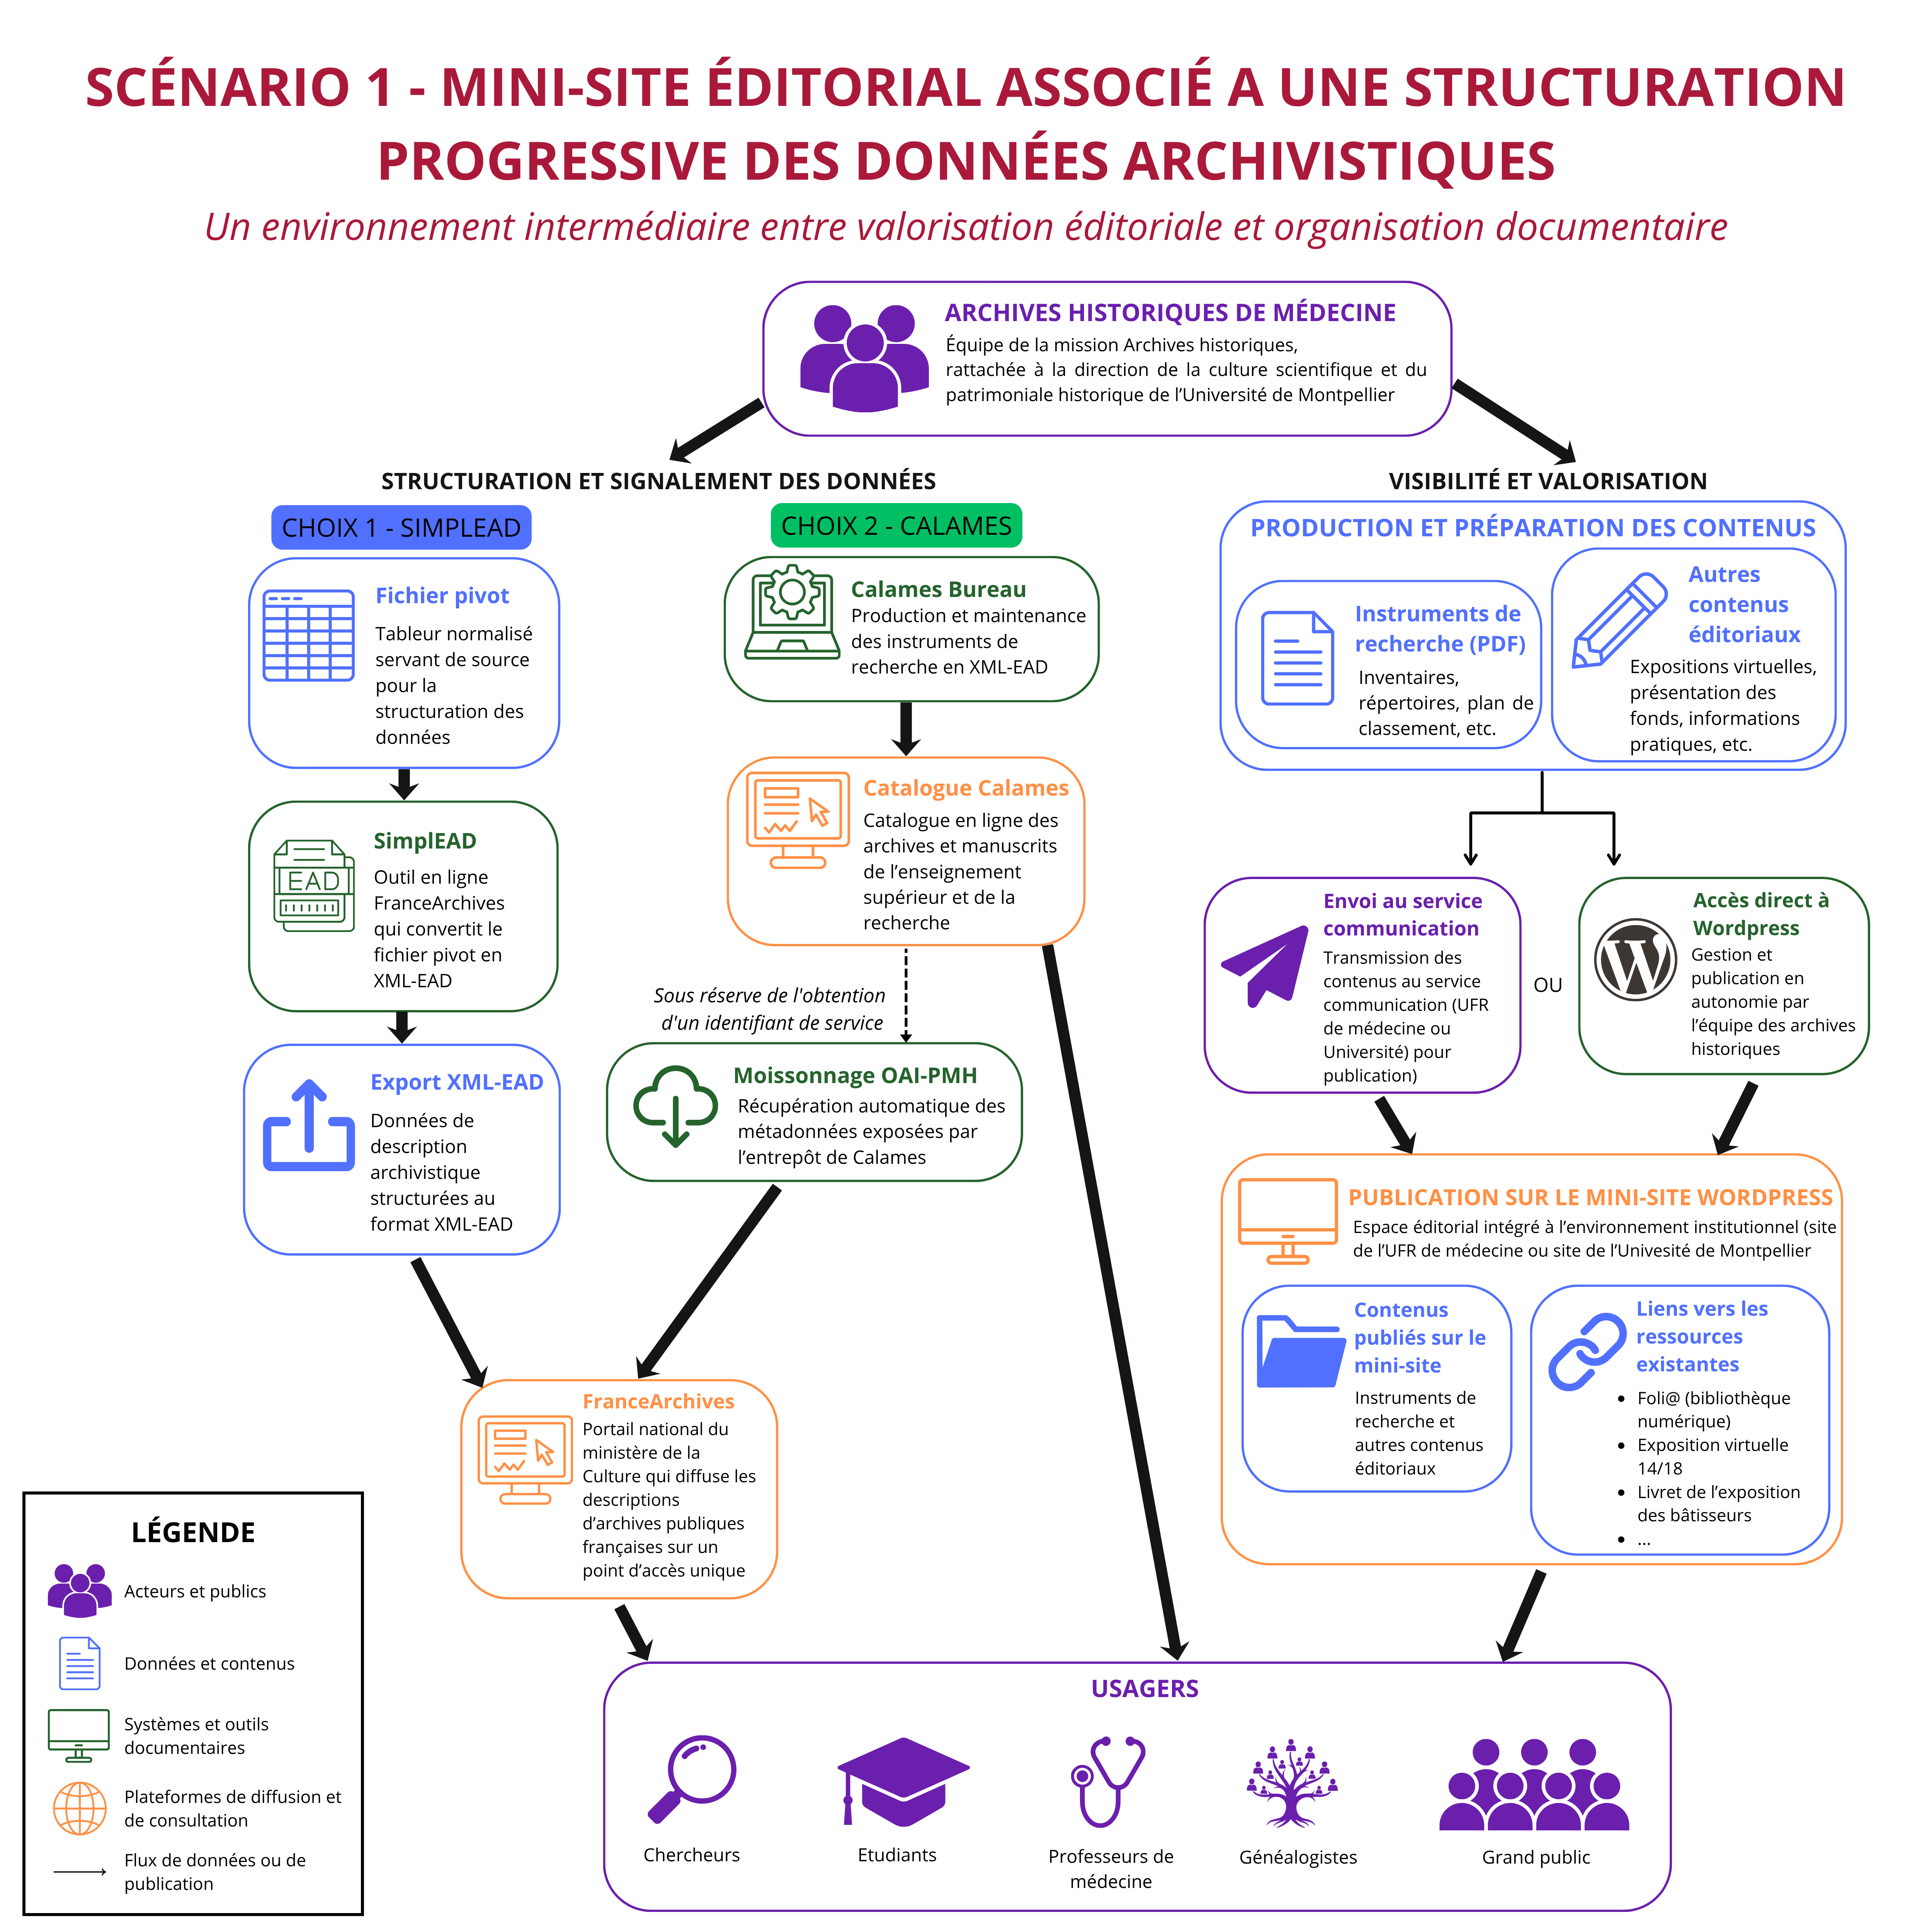
\includegraphics[
		width=\linewidth,
		height=1\textheight,
		keepaspectratio
		]{images/scenario1.png}
		\caption{Scénarios de structuration et de signalement des instruments de recherche et articulation avec le mini-site institutionnel}
		\label{fig:scenario1}
	\end{figure}
\end{landscape}

\chapter{Articulation des descriptions archivistiques et des reproductions numériques}
\label{chap:articulation-descriptions-reproductions}
\chapitrecourt{Descriptions et reproductions numériques}

La structuration et le \gls{signalement} des instruments de recherche ne constituent qu'une composante de la diffusion numérique des Archives historiques. La mise à disposition des reproductions exige également de déterminer où héberger les fichiers, comment les relier aux descriptions archivistiques et selon quelles modalités les rendre consultables. Production des descriptions, conservation des fichiers, exposition technique des images et restitution à l'usager peuvent ainsi relever de composants distincts.

Les essais conduits dans WordPress ont d'abord précisé les besoins auxquels un simple \gls{cms} ne répond pas. L'étude de Foli@ fournit ensuite un retour d'expérience sur une architecture associant gestion documentaire, \glspl{api}, services \gls{iiif} et visionneuse. À partir de ce modèle, le chapitre évalue les possibilités offertes par Flora, déjà acquis par l'Université, puis l'intérêt de Nakala comme entrepôt alternatif ou complémentaire pour les reproductions.


\section{Les besoins de consultation mis en évidence par le mini-site}
\label{sec:limites-cms-diffusion-documentaire}

\subsection{Les limites de la galerie et de l'affichage agrandi}

L'expérimentation conduite dans l'environnement WordPress de préproduction confirme les limites du \gls{cms} pour la diffusion documentaire. Pour restituer le \enquote{musée des archives}, les vingt-deux pièces sélectionnées ont d'abord été réunies au moyen du bloc \emph{Gallery}, qui permet d'afficher plusieurs images sous la forme d'une galerie et d'en paramétrer la disposition\footcite{WordPressGalleryBlock}. Sur la page générale, les reproductions apparaissent toutefois comme une succession de vignettes de petites dimensions (fig.~\ref{fig:musee-archives-wordpress-galerie}), ce qui donne une vue d'ensemble de la sélection mais uniformise des documents de formats et de natures différents et rend leur identification difficile lorsque les légendes sont longues.

\begin{figure}[htbp]
	\centering
	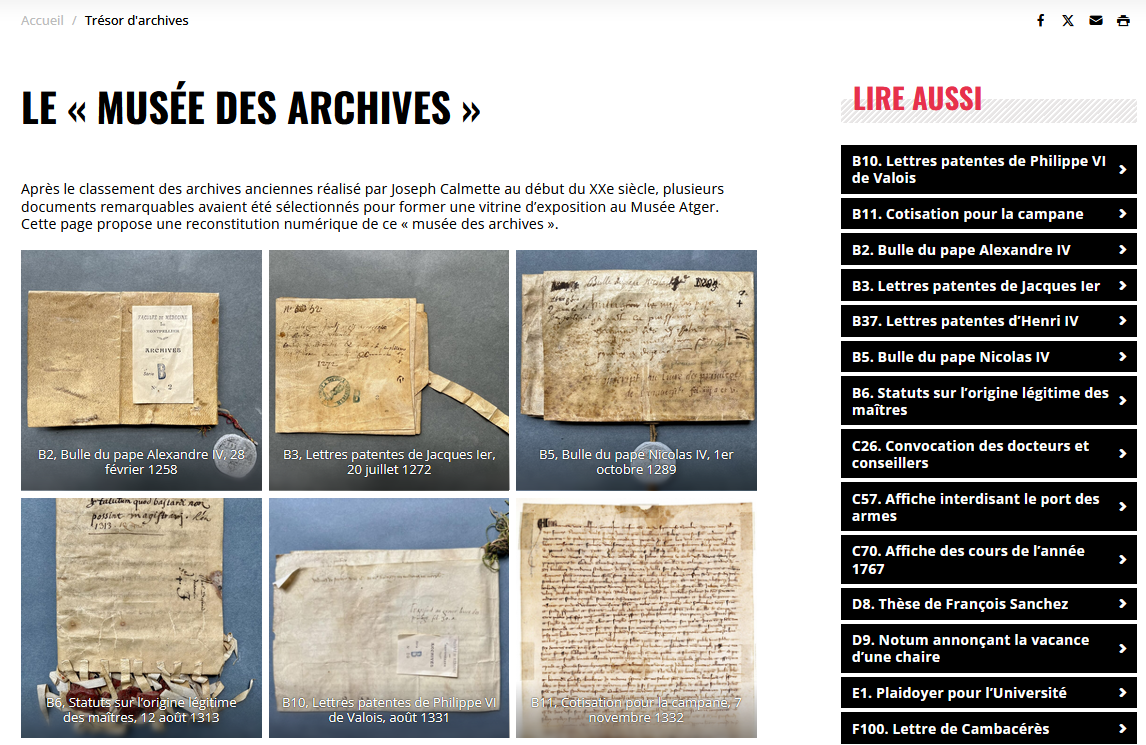
\includegraphics[width=0.92\textwidth]{images/museearchives_um_1.png}
	\caption[Présentation générale du \enquote{musée des archives} dans WordPress]
	{Présentation générale du \enquote{musée des archives} dans l'environnement WordPress de préproduction de l'Université de Montpellier : les reproductions et leurs légendes sont disposées sous la forme d'une succession de vignettes. Capture d'écran et redimensionnement : Clara Martin, août 2026}
	\label{fig:musee-archives-wordpress-galerie}
\end{figure}

L'ouverture d'une image déclenche un affichage agrandi en surimpression de la page (fig.~\ref{fig:musee-archives-wordpress-image}). Celui-ci conserve la légende associée au fichier, mais ne propose ni agrandissement progressif, ni déplacement dans l'image, ni sélection d'une zone précise. Peu gênante pour une illustration, cette limitation empêche l'examen détaillé de manuscrits, de registres ou de pièces de grand format.

\begin{figure}[htbp]
	\centering
	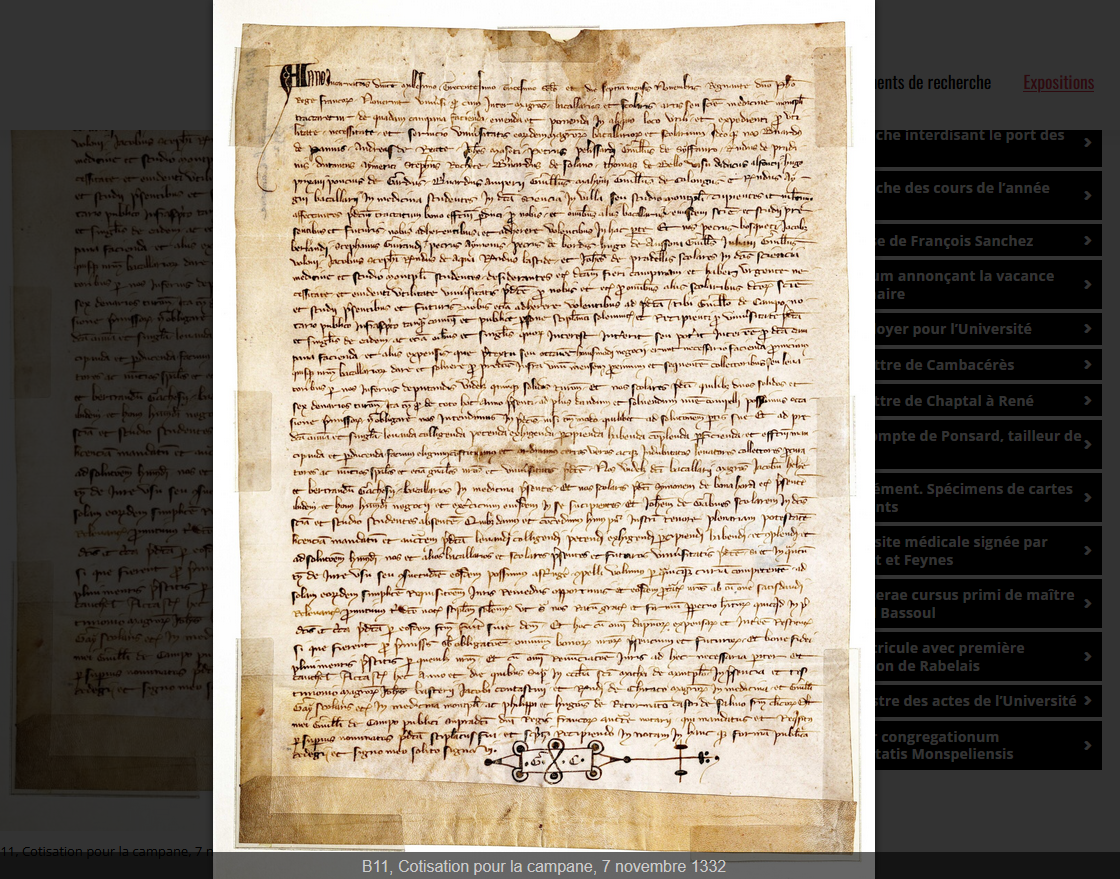
\includegraphics[
	width=0.78\textwidth,
	height=0.68\textheight,
	keepaspectratio
	]{images/museearchives_um_2.png}
	\caption[Affichage agrandi d'une reproduction dans WordPress]
	{Affichage agrandi de la pièce \texttt{B11}, \emph{Cotisation pour la campane}, dans l'environnement WordPress de préproduction : la légende demeure visible, mais l'image ne peut être ni agrandie ni déplacée. Capture d'écran et redimensionnement : Clara Martin, août 2026}
	\label{fig:musee-archives-wordpress-image}
\end{figure}

Lorsque plusieurs reproductions sont réunies sur une même page, des flèches latérales permettent de passer de l'une à l'autre, mais la légende disparaît dans la configuration testée (fig.~\ref{fig:musee-archives-wordpress-navigation}). La reproduction se trouve alors dissociée de sa cote, de son intitulé et de son analyse, comme sur la page consacrée aux trois spécimens de cartes d'étudiants de la série \enquote{Q Supplément}\footnote{Cette disparition ne constitue pas une impossibilité technique propre à WordPress, mais une limite du fonctionnement actuel de son dispositif d'agrandissement. Le problème est recensé dans le dépôt de développement de Gutenberg depuis 2024 : les légendes sont masquées dans la vue agrandie depuis WordPress 6.5 (\cite{WordPressGutenbergIssue60469}). Une proposition de modification ouverte en août 2026 prévoit d'afficher la légende correspondant à chaque image et de l'actualiser pendant la navigation au sein d'une galerie (\cite{WordPressGutenbergPR81500}). Une évolution du logiciel ou un développement spécifique du composant employé par l'Université pourrait donc corriger ce comportement, sous réserve des contraintes de maintenance de l'environnement institutionnel.}.

\begin{figure}[htbp]
	\centering
	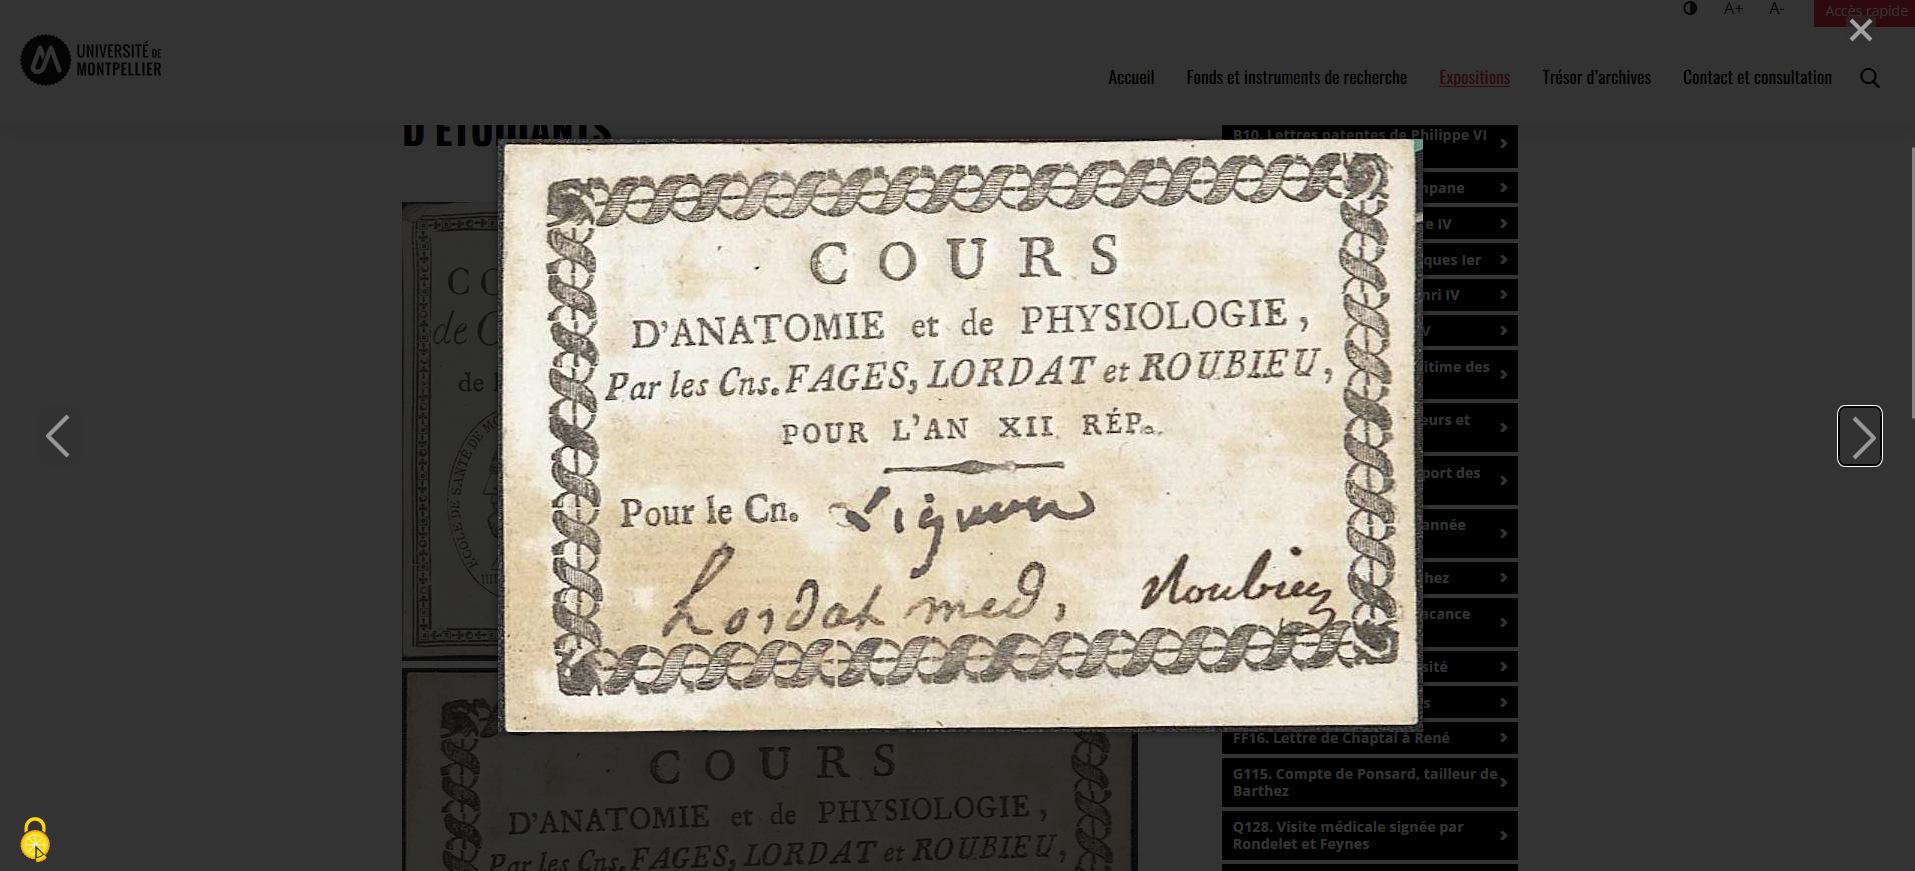
\includegraphics[width=\textwidth]{images/museearchives_um_3.png}
	\caption[Navigation entre plusieurs reproductions dépourvues de légende]
	{Navigation entre les trois reproductions réunies sur la page \enquote{Q Supplément. Spécimens de cartes d'étudiants} : les flèches permettent de passer d'une image à l'autre, mais la légende n'est plus affichée dans l'environnement WordPress testé. Capture d'écran et redimensionnement : Clara Martin, août 2026}
	\label{fig:musee-archives-wordpress-navigation}
\end{figure}

Ces essais ont conduit à utiliser la page générale du \enquote{musée des archives}, également accessible depuis la rubrique consacrée aux expositions, comme sommaire visuel : chaque vignette renvoie vers une page propre au document. Cette organisation alourdit la structure éditoriale, mais maintient l'association entre reproduction, cote, intitulé, date et texte de présentation ; elle ne remédie toutefois pas aux limites de consultation de l'image elle-même.


\subsection{Séparer la médiation des ressources documentaires}

La médiathèque WordPress permet de téléverser et de gérer les images, documents, fichiers audio et vidéo employés dans les contenus du site\footcite{WordPressMediaLibrary}. La taille maximale des fichiers dépend cependant de la configuration de l'hébergement, notamment des paramètres définis au niveau du serveur\footcite{WordPressMaxUploadSize}. Le volume des corpus, la définition nécessaire à leur examen et le besoin de réutiliser les objets numériques dans plusieurs interfaces excluent donc d'en faire le réservoir principal des images patrimoniales.

La même séparation vaut pour les descriptions : reproduire dans WordPress le contenu détaillé des instruments de recherche créerait une seconde version des données dont les corrections devraient être reportées dans plusieurs environnements. Le mini-site doit donc conserver des présentations synthétiques et renvoyer vers les descriptions structurées et les reproductions administrées ailleurs.


\subsection{Les conditions juridiques de la diffusion}

La mise en ligne ne peut être déduite de la seule communicabilité : la consultation d'un document dans un cadre contrôlé se distingue de sa diffusion publique, potentiellement indexable par les moteurs de recherche et accessible sans limitation, notamment lorsqu'il contient des données personnelles\footcite[pp.~99--101]{MalletPoujol2009}. Pour les fonds photographiques ou sonores, la détention du support doit en outre être distinguée des droits autorisant son exploitation ; selon les documents, la publication peut engager les droits de l'auteur ainsi que ceux des personnes ou des œuvres représentées\footcite[pp.~71--76]{Dieuzeide1998}. Chaque corpus devra donc faire l'objet d'une analyse précisant le statut juridique des documents, les titulaires et l'étendue des droits cédés, la présence éventuelle de données protégées, les crédits obligatoires et les conditions de consultation ou de réutilisation des fichiers.

L'expérimentation délimite ainsi le rôle du mini-site : assurer la médiation et organiser l'accès aux ressources, tandis que leur administration et leur consultation approfondie relèvent d'outils spécialisés. Foli@ fournit à l'échelle montpelliéraine un exemple de cette répartition fonctionnelle.


\section{Foli@ : l'évolution d'une bibliothèque numérique patrimoniale universitaire}
\label{sec:retour-experience-folia}

Foli@ est la bibliothèque numérique publique d'un environnement construit autour de Flora, progiciel web de gestion et de valorisation des collections patrimoniales permettant de centraliser données descriptives, données de gestion et ressources numériques\footcite{FloraLogicielGestion}. Son évolution fournit un retour d'expérience local sur l'organisation technique nécessaire à l'administration, à la diffusion et à la consultation de collections numérisées. Il ne s'agit pas d'en reproduire l'infrastructure pour les Archives historiques, mais d'en comprendre l'\gls{architecture-documentaire}\footnote{La politique patrimoniale du \gls{scdi} et ses projets transversaux seront examinés dans la partie~\ref{part:ecosysteme-patrimonial}.}.


\subsection{De la gestion des corpus à leur diffusion dans plusieurs réseaux}

Les universités montpelliéraines disposent avec Foli@ d'une bibliothèque numérique patrimoniale dont la numérisation et la diffusion sont assurées par le \gls{scdi}\footcite{SCDIFolia}. Créé en 2021 lors de la réorganisation consécutive à la fin de la Bibliothèque interuniversitaire de Montpellier, celui-ci exerce notamment des missions de coopération en matière d'informatique documentaire et de patrimoine écrit\footcite{SCDI2021}. Foli@ rassemble plus de 6\,500 documents numérisés répartis en neuf corpus thématiques : manuscrits médiévaux, imprimés anciens du XV\textsuperscript{e} au XIX\textsuperscript{e} siècle relatifs notamment à l'histoire de la médecine, de la pharmacie et de la botanique, cartes et plans, vues d'optique ou documents consacrés aux arts du cirque\footcite{Vanjak2026}.

Leur gestion repose sur Flora, employé par le \gls{scdi} depuis la fin des années 2000. Le logiciel administre les \glspl{metadonnees}, les fichiers numériques et les relations entre les notices, les reproductions, leur pagination et leur ordre de consultation\footnote{Entretiens avec Hélène Lorblanchet, Marie Nikichine, Audrey Cogoluègnès et Guenno Marti, Service de coopération documentaire interuniversitaire de Montpellier, 12 mai 2026, et avec Audrey Cogoluègnès, Marie Nikichine, Guenno Marti et Sébastien Leyreloup, 10 juillet 2026.}. Également employé pour les thèses de doctorat, les thèses d'exercice et les mémoires, Flora a été adapté aux collections patrimoniales par une modification du back-office au début des années 2010, puis par l'ajout de tables et de champs spécifiques à partir de 2014.

Foli@ complète plusieurs dispositifs de \gls{signalement} : ses ressources sont, dans leur quasi-totalité, également accessibles depuis le catalogue des bibliothèques universitaires de Montpellier, le Sudoc, Calames, Gallica ou Isidore\footcite{Vanjak2026}. Certaines notices de Calames renvoient ainsi vers une numérisation consultable dans Foli@. La refonte mise en production en juin 2026 accentue cette circulation entre plusieurs environnements en séparant l'administration des ressources de leur restitution publique.


\subsection{La refonte de 2026 : séparer gestion documentaire, interface publique et visionneuse}

\paragraph{Du portail Flora à une interface Drupal distincte}

Jusqu'en juin 2026, Foli@ était diffusée au moyen du portail public de Flora, qui assurait à la fois une fonction de \gls{ged}, par l'administration des fichiers et de leurs \glspl{metadonnees}, et leur restitution publique. Les collections étaient présentées selon une logique proche de celle d'un catalogue, sous forme de listes de résultats, de facettes et de vignettes. Certaines images apparaissaient comme des résultats individualisés, accompagnées d'informations sur le document auquel elles appartenaient, sa cote, sa date, le folio concerné ou les caractéristiques de la reproduction (fig.~\ref{fig:folia-ancienne-interface}).

\begin{figure}[htbp]
	\centering
	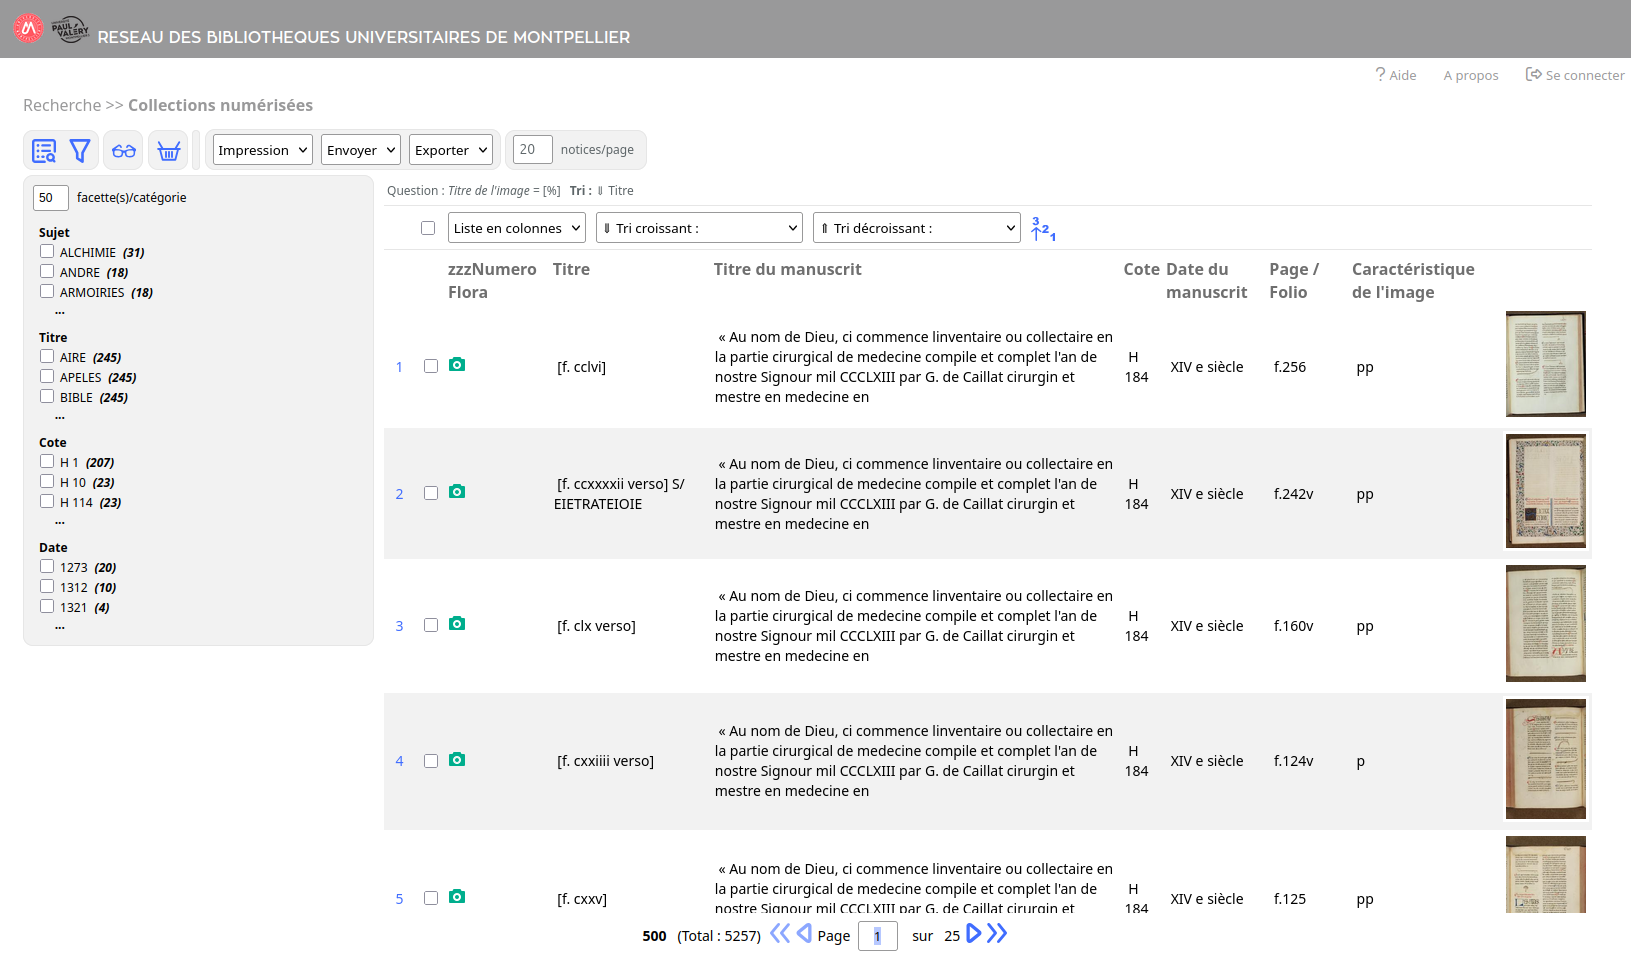
\includegraphics[
	width=\textwidth,
	height=0.72\textheight,
	keepaspectratio
	]{images/folia_ancienne_interface.png}
	\caption{Ancienne interface de diffusion des collections numérisées dans le portail Flora : affichage d'images sous forme de liste de résultats. Capture d'écran recadrée afin de rendre lisible la zone de l'interface concernée}
	\label{fig:folia-ancienne-interface}
\end{figure}

À l'échelle d'un document, la visionneuse native permettait de parcourir les reproductions dans l'ordre enregistré dans Flora. Les relations entre document, images, pagination et séquence existaient donc déjà dans le modèle documentaire, mais leur restitution demeurait liée à son interface.

Le rapport d'activité de 2021 décrit encore une chaîne dans laquelle les documents étaient numérisés, chargés dans la \gls{ged} Flora, sauvegardés puis mis en ligne dans Foli@, parallèlement à la préparation des \glspl{metadonnees} destinées au logiciel\footcite{SCDI2021}. Le plan d'action pour 2023 distingue ensuite l'intégration de nouveaux corpus, l'évolution de l'interface de Foli@ et l'archivage de la \gls{ged}, faisant apparaître une évolution séparée de l'environnement de gestion et de sa restitution publique\footcite{SCDI2022}.

Cette évolution aboutit en juin 2026 à une nouvelle instance de Foli@ : les corpus, leurs \glspl{metadonnees} et leurs fichiers demeurent administrés dans Flora, tandis qu'un site distinct développé sous \gls{drupal} assure leur diffusion\footcite{Vanjak2026}. Ce \gls{cms} permet au \gls{scdi} de faire évoluer la navigation et les contenus éditoriaux sans remplacer le socle documentaire. La page d'accueil associe ainsi moteur de recherche, accès aux corpus, actualités, contenus de présentation et informations sur la bibliothèque numérique (fig.~\ref{fig:folia-nouvelle-accueil}).

\begin{figure}[htbp]
	\centering
	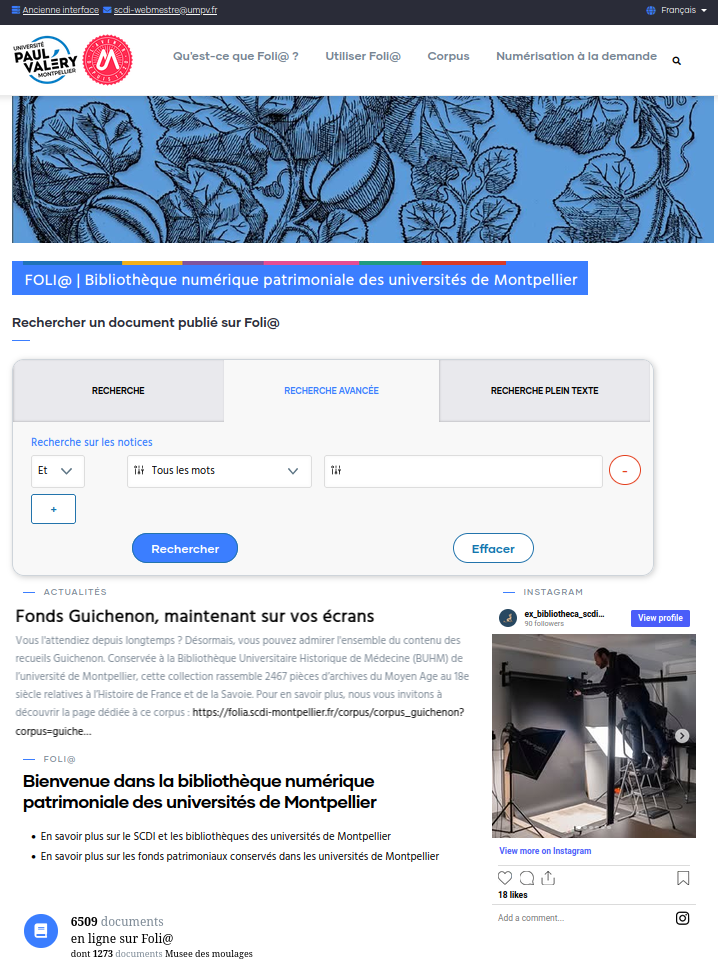
\includegraphics[
	width=0.72\textwidth,
	height=0.72\textheight,
	keepaspectratio
	]{images/folia_nouvelle_interface_1.png}
	\caption{Page d'accueil de la nouvelle interface de Foli@ mise en production en juin 2026. Capture d'écran recadrée afin de rendre lisible la zone de l'interface concernée}
	\label{fig:folia-nouvelle-accueil}
\end{figure}

L'aide distingue une recherche simple ou avancée sur les \glspl{metadonnees}, une recherche en plein texte dans les imprimés numérisés et une recherche par corpus à partir d'index dédiés. Les résultats peuvent être affinés par auteurs, corpus, dates, types documentaires, sujets ou localisations ; chaque entrée regroupe le titre, la date, la cote, le lieu de conservation et le type documentaire (fig.~\ref{fig:folia-nouvelle-resultats}).

\begin{figure}[htbp]
	\centering
	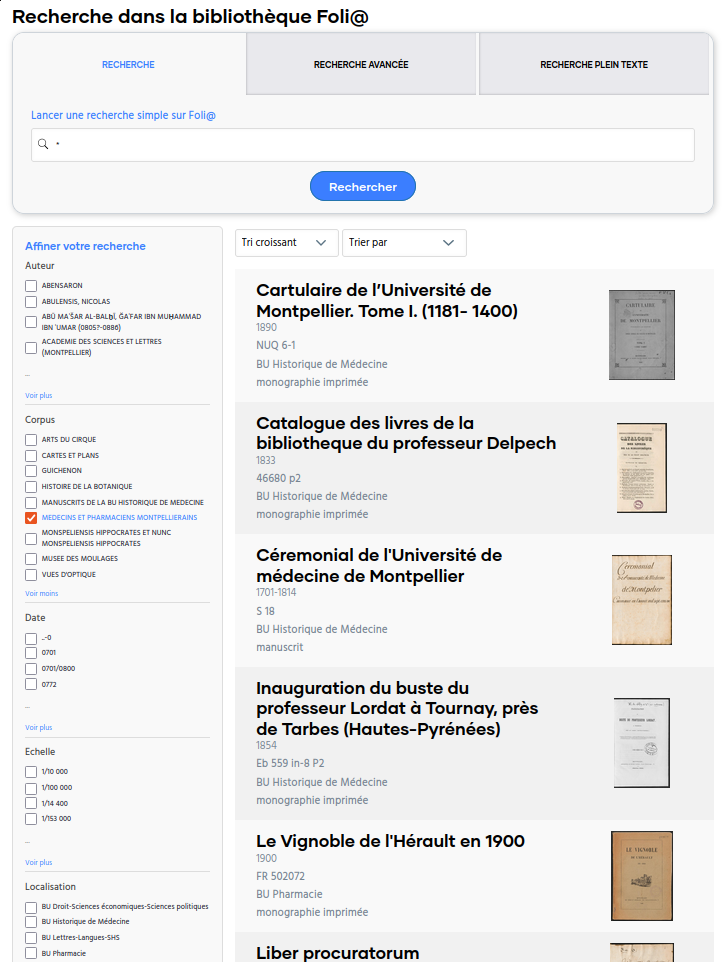
\includegraphics[
	width=\textwidth,
	height=0.72\textheight,
	keepaspectratio
	]{images/folia_nouvelle_interface_2.png}
	\caption{Affichage des résultats de recherche dans la nouvelle interface de Foli@ mise en production en juin 2026. Capture d'écran recadrée afin de rendre lisible la zone de l'interface concernée}
	\label{fig:folia-nouvelle-resultats}
\end{figure}

La consultation des reproductions est quant à elle confiée à \gls{mirador}, selon les standards \gls{iiif}. La nouvelle Foli@ répartit donc entre Flora, \gls{drupal} et \gls{mirador} les fonctions auparavant plus étroitement réunies.


\subsection{IIIF et Mirador : exposer, structurer et restituer les reproductions}

La séparation observée dans Foli@ correspond au problème auquel \gls{iiif} a été conçu pour répondre. Les bibliothèques numériques ont longtemps associé étroitement dépôts d'images, serveurs et applications de consultation, créant des environnements propres à chaque institution et limitant la réutilisation des ressources\footcite{SnydmanSandersonCramer2015}. Les \glspl{api} communes de \gls{iiif} permettent au contraire de rendre les images et les informations nécessaires à leur présentation accessibles à plusieurs applications sans déplacer les fichiers vers chacune d'elles.

Cette logique est mise en œuvre selon des modalités différentes dans les bibliothèques universitaires. À l'université Johns Hopkins, la \emph{Digital Library of Medieval Manuscripts} préexistante a été adaptée pour intégrer des visionneuses compatibles avec \gls{iiif} sans remplacer l'ensemble de son infrastructure ; à Harvard, les objets des collections numériques sont associés à des \glspl{manifeste-iiif} ouvrables dans différentes visionneuses et réutilisables dans d'autres environnements\footcite{ChenZhang2021IIIF}.

\paragraph{L'Image API : exposer les fichiers}

L'\emph{IIIF Image API} agit au niveau du fichier image. Un serveur compatible lui associe un identifiant et répond à des \glspl{uri} normalisés dont les paramètres indiquent la région demandée, ses dimensions, son orientation, sa qualité et son format\footcite{IIIFImageAPI}\footcite{SnydmanSandersonCramer2015}. Une visionneuse peut ainsi obtenir l'image entière ou seulement la portion et la résolution nécessaires à l'affichage : l'\gls{interoperabilite} porte ici sur l'accès technique à la ressource graphique.

\paragraph{La Presentation API : organiser les vues}

L'\emph{IIIF Presentation API} décrit dans un \gls{manifeste-iiif}, structuré en \gls{jsonld}, les \glspl{metadonnees} nécessaires à la présentation d'un objet et l'organisation de ses différentes vues\footcite{IIIFPresentationAPI}. Chaque page ou surface peut être représentée par un \emph{Canvas} auquel est associée sa reproduction : un registre numérisé page à page peut ainsi être restitué comme un objet ordonné plutôt que comme une juxtaposition de fichiers.

Cette fonction peut exploiter des relations déjà enregistrées dans le système documentaire. Dans Foli@, Flora connaissait avant l'adoption de \gls{iiif} l'appartenance des images à un document, leur pagination et leur ordre ; la \emph{Presentation API} permet désormais d'exprimer ces informations dans une ressource interprétable par d'autres applications. Elle ne remplace pas pour autant les standards de description documentaire : les descriptions plus riches peuvent demeurer dans leurs systèmes propres\footcite{SnydmanSandersonCramer2015}. Dans le domaine des archives, une expérimentation menée sur des fonds audiovisuels a ainsi montré que les objets \emph{Collection}, \emph{Manifest} et \emph{Canvas} peuvent correspondre à différents niveaux d'une structure archivistique et être reliés à une description en \gls{ead}\footcite{Critelli2026IIIFArchives}.

\paragraph{Mirador : interpréter les manifestes}

\gls{mirador} est une visionneuse web libre capable d'interpréter les \glspl{manifeste-iiif}, d'en restituer les vues et d'exploiter leurs structures de navigation\footcite{Mirador}. Conçue comme une application JavaScript configurable et extensible, elle peut être intégrée à une plateforme existante et afficher des ressources provenant de plusieurs environnements compatibles avec \gls{iiif}\footcite{WolffProbstBodenschatz2024}. La matrice maintenue par le consortium \gls{iiif} permet de vérifier la prise en charge par les différentes visionneuses des fonctionnalités de la \emph{Presentation API}\footcite{IIIFViewerMatrix3}, tandis que le \emph{IIIF Cookbook} fournit des exemples d'implémentation documentés pour construire et vérifier les \glspl{manifeste-iiif}\footcite{IIIFCookbook}.

FranceArchives exploite cette indépendance entre ressource et visionneuse pour intégrer dans ses notices des images \gls{iiif} hébergées par des services partenaires : les reproductions sont consultables dans \gls{mirador} ou Universal Viewer, tandis que leur contexte descriptif et le renvoi vers le site d'origine sont conservés\footcite{FranceArchivesIIIF2026}. Les recommandations élaborées avec Biblissima+ prévoient notamment des \glspl{uri} standardisés et pérennes pour les \glspl{manifeste-iiif} et les autres ressources \gls{iiif}, afin de permettre leur appel par des applications tierces\footcite{BiblissimaFranceArchivesIIIF2023}. Le mode multifenêtre de \gls{mirador} permet en outre de comparer des documents provenant d'un même fonds, de fonds différents ou d'institutions distinctes\footcite{FranceArchivesIIIF2026}.

Dans la nouvelle Foli@, \gls{drupal} appelle ainsi \gls{mirador}, tandis qu'un générateur développé autour de Flora produit les \glspl{manifeste-iiif} nécessaires à la consultation\footcite{Vanjak2026}\footnote{Échanges avec Audrey Cogoluègnès, Marie Nikichine, Guenno Marti et Sébastien Leyreloup, Service de coopération documentaire interuniversitaire de Montpellier, 10 juillet 2026.}.


\subsection{Les flux de données entre Flora et les autres systèmes}

La nouvelle architecture mobilise plusieurs mécanismes d'échange correspondant à des destinations distinctes. Pour alimenter \gls{drupal}, Flora expose des données par ses \glspl{api} \gls{rest}\footnote{Échanges avec Audrey Cogoluègnès, Marie Nikichine, Guenno Marti et Sébastien Leyreloup, Service de coopération documentaire interuniversitaire de Montpellier, 10 juillet 2026.}. Une \gls{api} est une interface par laquelle une application rend certaines de ses données ou fonctions accessibles à d'autres applications\footcite{CNILAPI}. \gls{rest}, pour \emph{Representational State Transfer}, désigne un style d'architecture appliqué aux services web : les ressources sont identifiées par des \glspl{uri}, interrogées au moyen du protocole \gls{http} et renvoyées sous une représentation qui peut notamment être encodée en \gls{json}\footcite{Fielding2000REST}. \gls{drupal} peut ainsi recevoir les \glspl{metadonnees} nécessaires à l'affichage sans accéder directement à la base interne du progiciel.

D'autres flux relient Flora aux réseaux documentaires : \gls{z3950}, protocole client--serveur normalisé pour l'interrogation de systèmes documentaires distants, assure les échanges avec le Sudoc\footcite{Lynch1997Z3950}, tandis que \gls{oaipmh} permet à un entrepôt d'exposer des lots de \glspl{metadonnees} récupérés périodiquement par un moissonneur et sert ici au \gls{signalement} dans Gallica\footcite{OAIPMH2002}\footnote{Entretien avec Hélène Lorblanchet, Marie Nikichine, Audrey Cogoluègnès et Guenno Marti, Service de coopération documentaire interuniversitaire de Montpellier, 12 mai 2026.}. Les services \gls{iiif}, examinés précédemment, assurent pour leur part l'exposition et la restitution des reproductions.

Le schéma élaboré par le \gls{scdi} replace ces différents flux dans l'environnement général de Flora (fig.~\ref{fig:schema-folia}). L'interface publique constitue ainsi l'aboutissement d'échanges entre plusieurs composants plutôt que le lieu où l'ensemble des données est stocké et administré.

\begin{figure}[htbp]
	\centering
	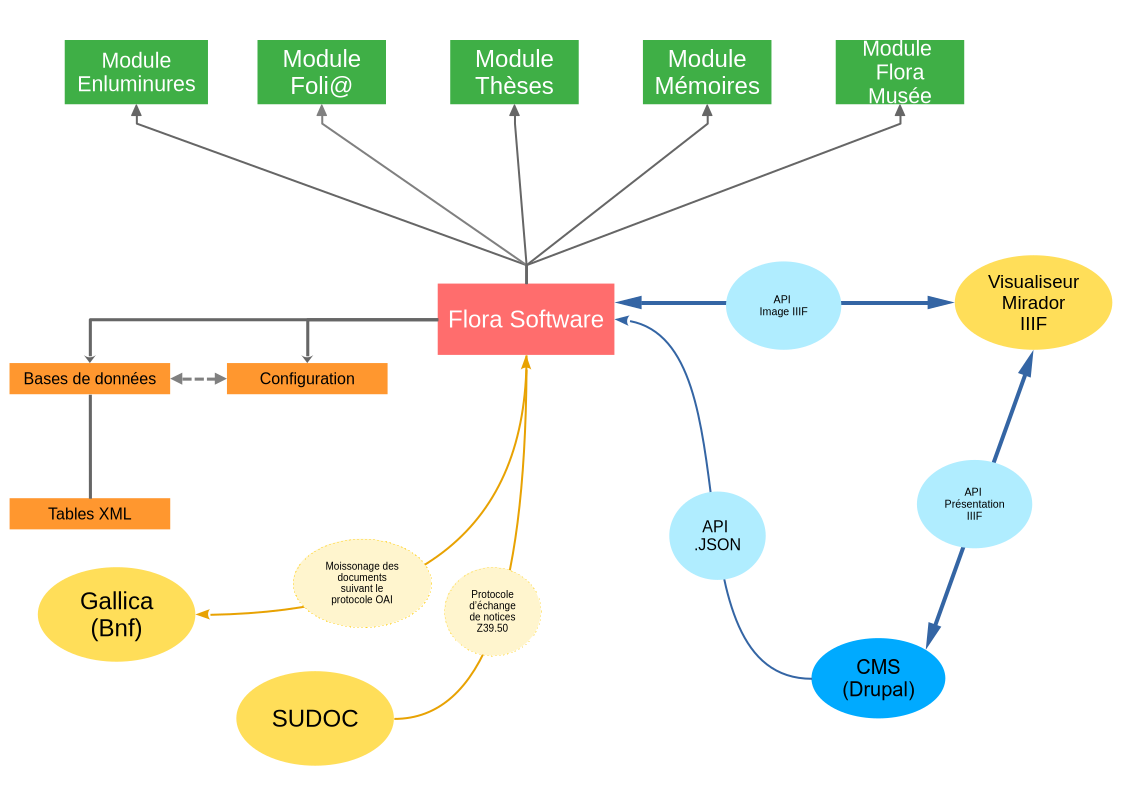
\includegraphics[
	width=\textwidth,
	height=0.78\textheight,
	keepaspectratio
	]{images/schema_folia.png}
	\caption{Architecture et flux de données de la nouvelle instance de Foli@ mise en production en juin 2026. Schéma élaboré par le Service de coopération documentaire interuniversitaire de Montpellier.}
	\label{fig:schema-folia}
\end{figure}


\subsection{Les développements propres à Foli@ : les limites d'une transposition aux archives}

Cette \gls{architecture-documentaire} résulte toutefois d'une construction progressive dans laquelle les fonctions standards de Flora ont été complétées par des paramétrages et des développements propres au \gls{scdi}\footnote{Échanges avec Audrey Cogoluègnès, Marie Nikichine, Guenno Marti et Sébastien Leyreloup, Service de coopération documentaire interuniversitaire de Montpellier, 10 juillet 2026.}. Dès 2014, des tables de concordance, de pagination et de granularité ainsi que des champs complémentaires ont été ajoutés pour structurer les relations entre notices et reproductions. Les images ne disposent pas de notices iconographiques autonomes : une table conserve principalement leur identifiant technique et leur numéro de page, tandis que d'autres établissent leur ordre et leur rattachement au document\footnote{Ibid.}. Antérieurs à l'adoption de \gls{iiif}, ces développements fournissent aujourd'hui les informations structurelles nécessaires à la construction des \glspl{manifeste-iiif}.

Le modèle documentaire a lui aussi été adapté. Le module Musée repose sur la notion de \enquote{bien}, insuffisante pour restituer toutes les informations bibliographiques d'un livre ancien ; un développement articule donc certaines données issues du Sudoc avec celles du module. La refonte de 2026 a en outre nécessité l'enrichissement des \glspl{api} \gls{rest}, la création de vues \gls{json} adaptées à \gls{drupal} et le développement du générateur de \glspl{manifeste-iiif} associant images, \glspl{metadonnees} et informations structurelles\footnote{Ibid.}. Ces trois développements --- articulation bibliographique, enrichissement des \glspl{api} et production des \glspl{manifeste-iiif} --- ont représenté des coûts distincts et compliquent les montées de version ; en juillet 2026, le \gls{scdi} n'avait ainsi pas encore adopté Flora 4.7\footnote{Ibid.}.

Ce retour d'expérience invite à transposer le principe de l'architecture plutôt que son implémentation locale. Les fonctionnalités de Foli@ ne peuvent être présumées dans le module Archives de la nouvelle instance Flora acquise par l'Université ; leur évaluation doit donc porter sur ce que cette dernière fournit nativement et sur les éventuelles adaptations qu'exigerait son emploi pour les Archives historiques.


\section{L'évaluation de la nouvelle instance Flora pour les Archives historiques}
\label{sec:flora-architecture-documentaire}

L'étude de Foli@ conduit à examiner séparément deux fonctions décisives dans la nouvelle instance Flora acquise par l'Université : la réutilisation des descriptions archivistiques hors du progiciel et l'association puis l'exposition des reproductions numériques.


\subsection{Un environnement de gestion déjà acquis à l'échelle de l'Université}

La nouvelle instance était en cours de déploiement au moment du stage et ne doit pas être confondue avec celle qui soutient Foli@, fondée sur le module Musée et sur des développements accumulés depuis les années 2010\footnote{Échanges avec Audrey Cogoluègnès, Marie Nikichine, Guenno Marti et Sébastien Leyreloup, Service de coopération documentaire interuniversitaire de Montpellier, 10 juillet 2026.}. La diffusion des futures numérisations des Archives historiques n'étant pas appelée, à ce stade, à rejoindre Foli@, l'évaluation a porté sur les fonctionnalités standards et le paramétrage du nouveau déploiement.

\paragraph{Un projet destiné à fédérer des collections hétérogènes}

Le projet concerne des archives, des collections scientifiques, techniques et naturelles, des objets artistiques et mobiliers, des collections de recherche et des spécimens vivants, jusqu'alors administrés au moyen d'outils et d'espaces de stockage distincts\footnote{\emph{Réunion de lancement du projet}, Flora Software -- Université de Montpellier, 14 février 2025.}. Le cahier des charges visait donc un \enquote{logiciel commun de gestion des collections} prenant en charge les beaux-arts, les archives, les collections de muséum, scientifiques et techniques ainsi que leur valorisation publique\footnote{Ibid.}. Le périmètre associe notamment les collections des services centraux, de l'Institut des sciences de l'évolution de Montpellier et des facultés de pharmacie et de médecine ; les premières estimations atteignaient plusieurs dizaines de milliers de notices et plus de cent mille pour le seul ISEM\footnote{Ibid.}.

Cette mutualisation documentaire se retrouve dans la \gls{dcsph}, où le Service du patrimoine historique gère les collections patrimoniales et scientifiques, tandis que le Service des archives historiques, scientifiques et administratives prend en charge les archives\footnote{L'organisation de la \gls{dcsph} est présentée en annexe~\ref{annexe:dcSPH}.}.

\paragraph{Un périmètre fonctionnel associant collections et archives}

Le marché, notifié en décembre 2024 et lancé en février 2025, porte sur une licence site perpétuelle couvrant l'ensemble de l'Université et un nombre illimité d'utilisateurs\footnote{\emph{Planning prévisionnel du projet Flora -- Université de Montpellier}, version 4 du 17 mars 2026}. Flora regroupe quatre grandes familles fonctionnelles : gestion des collections, catalogage des bibliothèques, description et gestion des archives, gestion des documents et des ressources numériques\footcite{FloraLogicielGestion}. À ce socle peuvent s'ajouter des fonctions spécialisées, notamment la gestion des périodiques et de la circulation des documents, Flora-Archéo, Flora-ImmoPat, les services d'\gls{interoperabilite} par \gls{api} et \gls{oaipmh}, ainsi que la gestion archivistique avancée\footcite{FloraProfilRCIP2025}.

L'Université n'a pas acquis l'ensemble de ces extensions. Le marché porte principalement sur Flora Musée et sur le niveau avancé de Flora Archives ; l'offre comprend également un portail public reposant sur des composants WordPress\footnote{\emph{Présentation de l'offre Flora Software à l'Université de Montpellier}, audition de négociation, 18 juillet 2024.}. Le niveau 1 permet de saisir et de rechercher des fonds, des versements et des unités d'archives, de les organiser hiérarchiquement et de les relier aux autorités, aux thésaurus et aux autres entités documentaires\footcite{FloraCatalogueFormations2024}. Le niveau 2, acquis par l'Université, complète cette description par la gestion avancée des localisations et délocalisations, des magasins et unités de conditionnement, des éliminations, des utilisateurs, des réservations et des communications en salle de lecture\footcite{FloraCatalogueFormations2024}. Le même environnement peut ainsi administrer versements, unités d'archives, plans de classement, localisations, conditionnements, éliminations et communications\footnote{\emph{Réunion de lancement du projet}, Flora Software -- Université de Montpellier, 14 février 2025.}.

L'acquisition comprend enfin l'installation et le paramétrage de Flora et du portail, des environnements de test et de production, la reprise des données, des \glspl{referentiel} et des images, leur validation et les formations. La solution est hébergée \emph{on premise}, sur les serveurs de l'Université. La reprise repose sur deux fichiers pivots, l'un destiné aux collections et l'autre aux archives ; après une phase d'essai sur quatre bases, les autres ensembles et leurs images doivent être progressivement intégrés par l'Université\footnote{Ibid.}.

\paragraph{Une association tardive des Archives historiques qui transforme l'enjeu du stage}

Le déploiement s'étend de 2025 à 2026 : installation et paramétrage, élaboration et test des fichiers pivots, reprise d'un ensemble de données plus complet, validation des imports, puis mise en production\footnote{\emph{Planning prévisionnel du projet Flora -- Université de Montpellier}, version 4 du 17 mars 2026.}. La \enquote{recette} désigne ici la vérification de la reprise des données et de la conformité fonctionnelle de l'application avant son passage en production.

Le projet associe notamment la \gls{dcsph}, la \gls{dsin} et des référents documentaires\footnote{\emph{Réunion de lancement du projet}, Flora Software -- Université de Montpellier, 14 février 2025.}. Une formation à la reprise des données a été organisée en juin 2025, puis des sessions générales en janvier 2026, une formation au module Archives les 27 et 28 janvier et une formation à son administration au début du mois de février\footnote{\emph{Planning prévisionnel du projet Flora -- Université de Montpellier}, version 4 du 17 mars 2026.}.

Le suivi archivistique avait été confié à Manon Guillermin, chargée des archives courantes et intermédiaires. Les Archives historiques n'avaient été associées ni à la préparation du marché ni aux négociations qui en avaient déterminé le périmètre ; elles ont rejoint le projet alors que le logiciel était déjà acquis et paramétré\footnote{Réunion de travail avec Sophie Dikoff, Emma Bertrand, Manon Guillermin et Véronique Bourgade, 21 avril 2026.}. Le stage devait donc vérifier l'adéquation aux fonds historiques d'un environnement déjà retenu, plutôt que spécifier un nouvel outil.


\subsection{Produire dans Flora des descriptions réutilisables hors du logiciel : le test de l'export EAD}

Les fichiers, scripts et résultats de cette expérimentation sont documentés dans un dépôt GitHub.\footnote{Le dépôt, les données de test, les exports produits par Flora, les rapports de validation et le script de correction sont présentés en annexe~\ref{annexe:analyse-flora}.}

\paragraph{De la reprise des données à l'export EAD}

Le fichier pivot consacré aux unités d'archives prévoit notamment la cote de versement, le type d'entité, le cadre de classement, le numéro d'article et son unité parente, le service versant et le producteur, les dates, le titre et l'analyse, l'indexation, les supports, la communicabilité, les renvois et les fichiers numériques associés\footnote{Fichier pivot d'import des unités d'archives transmis dans le cadre du projet Flora, version utilisée par l'Université de Montpellier en 2026.}.

Le versement constitue le niveau d'entrée, tandis que les niveaux inférieurs relèvent de la catégorie générique des \enquote{unités d'archives}. Celles-ci peuvent être qualifiées comme groupe d'articles, article, dossier, sous-dossier ou pièce et reliées par des relations parent--enfant\footnote{\emph{Module Archives -- Descriptif fonctionnel}, Flora Software, 22 juillet 2024.}. Le modèle interne permet donc de représenter une arborescence de type \emph{versement > groupe d'articles > article > dossier > sous-dossier > pièce}, sans imposer l'emploi de tous ces niveaux.

Les premiers essais ont précisé les correspondances relatives à l'état de traitement, au support, à l'état matériel, à la communicabilité et aux identifiants\footnote{Réunion de travail avec Sophie Dikoff, Emma Bertrand, Manon Guillermin et Véronique Bourgade, 21 avril 2026.}. Le fichier pivot reste toutefois un format de reprise initiale : son import dépend de champs obligatoires, d'identifiants cohérents et de listes de valeurs contrôlées ; les notices peuvent ensuite être enrichies dans l'interface\footnote{\emph{Rapport d'analyse. Phase 2. Reprise des données (fichier pivot) Archives}, Flora Software, juillet 2026.}.

L'enjeu principal concernait leur réutilisation dans Calames ou FranceArchives. Le mémoire technique annonçait à cette fin un \enquote{export \gls{xml}-\gls{ead} pour les données d'archives}\footnote{\emph{Mémoire technique}, Decalog, version 3.0, 28 avril 2024, p.~18.}\footcite{Sibille2012}. L'évaluation a donc porté sur la conformité syntaxique des fichiers à l'\gls{ead} 2002 et sur la restitution des relations hiérarchiques définies dans Flora.

\paragraph{Un export mêlant des structures EAD 1998 et EAD 2002}

L'export a d'abord été testé sur une structure minimale à plat composée d'un versement et de trois articles, puis sur des descriptions enrichies et plusieurs arborescences\footnote{Tests de l'export \gls{xml}-\gls{ead} du module Archives de Flora réalisés dans le cadre du stage, printemps et été 2026.}.

Flora établit des correspondances avec plusieurs éléments spécialisés de l'\gls{ead} : \texttt{<origination>} pour le producteur, \texttt{<unitdate>} pour les dates, \texttt{<scopecontent>} pour l'analyse, \texttt{<accruals>} pour les accroissements, \texttt{<bibliography>} pour la bibliographie, \texttt{<odd>} pour les notes et \texttt{<physdesc>} pour le métrage. Le modèle interne contient donc une part importante des informations attendues dans un instrument de recherche.

Les fichiers exportés déclarent explicitement l'utilisation de la gls{dtd} \gls{ead} 2002 et ont donc été contrôlés contre celle-ci\footnote{Une DTD (\emph{Document Type Definition}) définit les éléments, attributs, relations hiérarchiques et modèles de contenu autorisés dans un document XML.}. Aucun des fichiers testés n'est cependant conforme à cette DTD ; le cas minimal à plat, c'est-à-dire un versement contenant trois articles directement rattachés, sans dossier, sous-dossier ni autre niveau hiérarchique intermédiaire, restitue correctement les trois unités et leurs identifiants sans duplication, mais produit déjà vingt-neuf erreurs de validation.

Une partie de ces écarts semble provenir d'un mélange entre des structures relevant de versions différentes de l'\gls{ead}. Les éléments \texttt{<admininfo>} et \texttt{<add>} appartiennent à la première version d'\gls{ead} publiée en 1998 mais ne figurent plus comme éléments dans la \gls{dtd} \gls{ead} 2002 pourtant déclarée par l'export. Leur présence suggère que le générateur conserve des structures héritées d'\gls{ead} 1998. L'élément \texttt{<unititle>} relève d'un problème différent : il n'est pas reconnu par la \gls{dtd} \gls{ead} 2002, qui attend \texttt{<unittitle>}.

D'autres erreurs concernent des éléments appartenant bien à \gls{ead} 2002 mais dont Flora ne respecte pas le modèle de contenu. Du texte ou des éléments sont placés directement dans \texttt{<otherfindaid>}, \texttt{<acqinfo>} et \texttt{<accessrestrict>} alors que la DTD attend une structuration interne déterminée ; certains blocs \texttt{<did>} ne contiennent en outre qu'un élément \texttt{<head>} sans les éléments descriptifs attendus.

\begin{table}[htbp]
	\centering
	\small
	\begin{tabular}{p{0.72\textwidth}r}
		\toprule
		\textbf{Principales erreurs du test minimal à plat} & \textbf{Occurrences} \\
		\midrule
		Contenu non structuré dans \texttt{<otherfindaid>} & 4 \\
		\texttt{<admininfo>} et \texttt{<add>} non reconnus & 4 + 4 \\
		Structure incorrecte de \texttt{<acqinfo>} & 4 \\
		Structure incorrecte de \texttt{<accessrestrict>} & 4 \\
		Bloc \texttt{<did>} insuffisamment structuré & 3 \\
		\texttt{<unititle>} au lieu de \texttt{<unittitle>} & 1 \\
		\bottomrule
	\end{tabular}
	\caption{Principales erreurs relevées lors de la validation de l'export EAD minimal à plat produit par Flora}
	\label{tab:flora-export-ead-minimal}
\end{table}

Les descriptions enrichies mobilisent davantage d'éléments spécialisés de l'\gls{ead}, notamment \texttt{<custodhist>}, \texttt{<appraisal>}, \texttt{<language>} et \texttt{<langusage>}, mais font apparaître de nouvelles erreurs de structure, notamment dans \texttt{<profiledesc>}, \texttt{<custodhist>} et \texttt{<appraisal>}\footnote{Ibid.}. Certaines informations de gestion sont également répétées entre le versement et ses unités enfants.

Les niveaux locaux sont exportés dans des composants \texttt{<c level="otherlevel">}. Cette syntaxe peut être valide si la valeur locale est correctement exprimée, mais son \gls{interoperabilite} dépend de la capacité de l'application destinataire à interpréter les niveaux propres à Flora.

\paragraph{Une restitution défectueuse des hiérarchies}

Les tests hiérarchiques ont révélé une anomalie distincte : une structure composée d'un article et de deux dossiers devait produire trois composants, mais en exportait cinq ; une arborescence à trois niveaux produisait six composants pour trois unités et deux branches article--dossier six composants pour quatre unités\footnote{Ibid.}. Chaque unité enfant est exportée comme composant autonome puis à nouveau sous son parent ; la duplication se cumule avec la profondeur et réemploie les mêmes identifiants à plusieurs emplacements.

L'anomalie porte ainsi sur la sérialisation des relations enregistrées dans Flora. Or la position d'une unité dans l'arborescence participe directement de son contexte archivistique : un fichier qui duplique les composants ne peut être transmis tel quel à une application destinataire, même si les notices individuelles sont correctement renseignées.

\paragraph{Une correction automatisée possible, mais non pérenne}

L'aplatissement des descriptions ou la multiplication des versements aurait limité les duplications au prix d'une perte de structure ; l'export simultané de plusieurs versements a par ailleurs produit une archive ZIP vide\footnote{Ibid.}. Ce comportement peut être propre à l'instance de préproduction testée, mais empêchait de retenir ce contournement.

Un script Python a été développé pour corriger le fichier minimal. Il remplace \texttt{<unititle>} par \texttt{<unittitle>}, supprime les enveloppes \texttt{<admininfo>} et \texttt{<add>} tout en conservant leur contenu, restructure \texttt{<otherfindaid>}, \texttt{<accessrestrict>} et \texttt{<acqinfo>} et complète les blocs \texttt{<did>} insuffisamment structurés\footnote{Test de correction automatisée de l'export \gls{xml}-\gls{ead} de Flora réalisé dans le cadre du stage, août 2026.}. Après transformation, le fichier minimal valide contre la \gls{dtd} \gls{ead} 2002, ce qui montre qu'une partie des anomalies suit des règles régulières pouvant être corrigées automatiquement.

Une telle transformation ne constitue toutefois pas une chaîne pérenne : il faudrait étendre les règles aux descriptions enrichies, reconstruire les hiérarchies, contrôler les valeurs locales et maintenir le script lors des évolutions de Flora. Le retour du \gls{scdi} montre précisément que les développements spécifiques doivent être testés lors des montées de version\footnote{Échanges avec Audrey Cogoluègnès, Marie Nikichine, Guenno Marti et Sébastien Leyreloup, Service de coopération documentaire interuniversitaire de Montpellier, 10 juillet 2026.}. Produire l'\gls{ead} à partir d'un export CSV, Excel ou \gls{json} déplacerait cette charge de transformation sans la supprimer\footnote{Point de travail avec Manon Guillermin sur Flora, 2 juin 2026.}.

La production de l'\gls{ead} a donc été dissociée des autres fonctions envisagées pour Flora, au profit d'outils dans lesquels ce format constitue directement le format de travail ou d'échange, notamment SimplEAD et Calames. Le constat reste circonscrit à l'instance de préproduction testée en 2026 : Flora permet de centraliser les données archivistiques, de les rechercher, d'établir des relations entre unités et d'associer de nombreux champs au vocabulaire \gls{ead}, mais aucun fichier contrôlé ne valide en l'état et les arborescences produisent des composants dupliqués.

L'export \gls{ead} figure dans la documentation contractuelle, mais aucun usage régulier n'a pu être identifié dans les retours recueillis. Ces résultats ne préjugent donc ni d'une correction ni d'une évolution ultérieure du logiciel ; ils établissent qu'au moment du test, l'instance disponible ne produisait pas une chaîne \gls{ead} directement exploitable pour un versement dans Calames ou un \gls{signalement} dans FranceArchives.

\paragraph{Le retour du Musée des Confluences : distinguer gestion locale et signalement national}

Le Musée des Confluences utilise Flora parce que le logiciel était déjà employé pour les collections, permettait de mutualiser les autorités et les thésaurus et offrait à une archiviste seule un environnement commun de centralisation. Les descriptions y sont largement organisées à plat et rattachées aux entrées ou aux versements ; les fonctions de recherche en plein texte et par autorités sont en revanche jugées satisfaisantes\footnote{Entretien avec Pauline Laugraud et Jérémie Léonard, Musée des Confluences de Lyon, 4 juin 2026.}. Le portail public permet d'associer aux notices des instruments de recherche sous forme de fichiers PDF joints\footnote{\emph{Portail des collections et des archives du Musée des Confluences}, rubrique Archives, consulté le 11 août 2026.}.

Cette organisation ne résout pas l'\gls{interoperabilite} : les échanges engagés avec FranceArchives n'ont pas abouti à une correspondance satisfaisante, les exports \gls{xml} ne constituent pas nécessairement des instruments \gls{ead} directement exploitables et le flux OAI en Dublin Core restitue les données à plat\footnote{Entretien avec Pauline Laugraud et Jérémie Léonard, Musée des Confluences de Lyon, 4 juin 2026.}. Ce retour confirme donc qu'un logiciel peut demeurer pertinent pour la gestion et la diffusion locale de notices sans constituer l'outil de production de l'instrument destiné au \gls{signalement} national.


\subsection{Associer les reproductions dans Flora et les exposer hors du logiciel}

L'échec de l'export \gls{ead} directement exploitable n'écarte pas Flora de l'\gls{architecture-documentaire}. Une seconde série de vérifications a porté sur sa capacité à administrer les reproductions et à les rendre accessibles à d'autres composants.

\paragraph{Associer les fichiers aux unités d'archives}

Flora 4.7 permet d'associer des fichiers, notamment JPEG et PDF, aux versements et aux unités d'archives et prévoit leur import. Le fichier pivot comporte un champ de localisation du document numérique, complété par des informations saisissables dans la notice\footnote{\emph{Questions Flora -- fichiers pivot archives : intégration fonds archives historiques et fonds iconographiques}, réponses de Marielle Gidon et Chantal Jamot, Flora Software, 2026.}.

Dans le module Archives, le fichier associé ne possède toutefois pas de notice documentaire autonome. Cette organisation limite la granularité descriptive lorsqu'une unité comprend plusieurs reproductions : chaque fichier ne peut recevoir séparément une cote, un titre, une date ou des \glspl{metadonnees} équivalentes. Un registre numérisé page à page exige pourtant d'ordonner les vues et, si nécessaire, de les documenter individuellement. Le module Musée peut gérer des images individualisées dans son réservoir photographique, mais cette structuration n'est pas celle des fichiers associés aux unités d'archives.

\paragraph{Identifier, décrire et exposer les ressources}

Le mémoire technique mentionne trois mécanismes complémentaires : des \glspl{identifiant-perenne} \gls{ark} pour les notices et documents associés, des \glspl{api} \gls{rest} exposant des données en \gls{json} et un serveur d'images compatible \gls{iiif}\footnote{\emph{Mémoire technique}, Decalog, version 3.0, 28 avril 2024.}. Flora Software a confirmé que les documents associés aux archives peuvent recevoir un \gls{ark} et que des vues \gls{json} existent pour les entrées et les unités d'archives\footnote{Échanges avec Marielle Gidon et Chantal Jamot, Flora Software, juillet 2026.}. Ces mécanismes permettent respectivement de maintenir une adresse stable, de récupérer les données descriptives et d'accéder aux images depuis une application extérieure, selon le principe de découplage sur lequel repose \gls{iiif}\footcite{SnydmanSandersonCramer2015}.

La présence d'un fichier dans Flora n'entraîne cependant pas sa publication. Dans la configuration acquise par l'Université, le futur portail public, dont la mise en ligne est prévue à partir de la fin de l'année 2026, doit permettre la restitution des collections muséales, mais la publication des données du module Archives n'est pas prévue dans cette interface\footnote{Échanges avec Marielle Gidon et Chantal Jamot, Flora Software, juillet 2026.}. Flora permet en revanche un accès direct aux données archivistiques au moyen de profils et d'habilitations, logique adaptée à la gestion et à la consultation contrôlée des archives courantes et intermédiaires plutôt qu'à leur diffusion dans un portail patrimonial public.

L'association d'un fichier à une unité, son exposition technique et sa publication doivent donc être distinguées. FranceArchives fournit un précédent : des images \gls{iiif} hébergées par des services partenaires peuvent être consultées dans ses propres notices sans être recopiées sur le portail\footcite{FranceArchivesIIIF2026}. Flora pourrait de la même manière demeurer le système administrant les reproductions des Archives historiques tandis que leur consultation interviendrait dans une interface extérieure.

\paragraph{Produire les manifestes en dehors de Flora si le module Archives ne les génère pas}

L'exposition des fichiers par l'\emph{IIIF Image API} doit être complétée, pour les objets comportant plusieurs vues, par un \gls{manifeste-iiif} conforme à la \emph{Presentation API}. Dans Foli@, cette fonction est assurée par un générateur développé spécifiquement pour la nouvelle chaîne de diffusion, dont la réalisation a représenté un coût supplémentaire et qui repose sur des développements propres à l'instance Flora du \gls{scdi}\footnote{Échanges avec Audrey Cogoluègnès, Marie Nikichine, Guenno Marti et Sébastien Leyreloup, Service de coopération documentaire interuniversitaire de Montpellier, 10 juillet 2026.}.

Si le module Archives ne produit pas lui-même ces \glspl{manifeste-iiif}, une possibilité consiste à intercaler une couche logicielle intermédiaire, ou \gls{middleware}, entre Flora et la visionneuse. Le dispositif mis en œuvre pour arthistoricum.net en fournit un exemple : lorsqu'un \gls{manifeste-iiif} est demandé, le \gls{middleware} interroge les systèmes contenant les \glspl{metadonnees}, récupère les informations relatives aux images puis construit la ressource transmise à \gls{mirador}\footcite{WolffProbstBodenschatz2024}.

Appliqué aux Archives historiques, ce composant devrait récupérer par les \glspl{api} de Flora les \glspl{metadonnees} de l'unité, les identifiants de ses fichiers et les informations permettant d'en déterminer la séquence, puis construire le \gls{manifeste-iiif} et ses \emph{Canvas}. Celui-ci pourrait être généré à la demande ou préalablement et publié comme ressource statique sur un serveur web\footcite{BiblissimaIIIFImplementation}\footcite{IIIFManifestGeneration}. Le \emph{IIIF Cookbook} fournit les structures de référence permettant de construire et de vérifier les \glspl{manifeste-iiif} ainsi produits\footcite{IIIFCookbook}.

Un tel \gls{middleware} peut prendre la forme d'un service ou d'un script plutôt que d'un nouveau progiciel, mais constitue néanmoins un développement à maintenir. Sa faisabilité dépend surtout des données exposées par Flora : il faut pouvoir identifier les fichiers rattachés à une unité et en restituer l'ordre. Les tables spécifiques utilisées à cette fin dans Foli@ ne peuvent être présumées dans le module Archives. La production externe des \glspl{manifeste-iiif} ne serait donc pertinente que si les \glspl{api} donnent accès aux informations nécessaires ; son coût devrait alors être comparé à celui d'un générateur intégré au progiciel.


\section{Nakala comme entrepôt alternatif pour les reproductions}
\label{sec:nakala-reproductions}

Si Flora ne permet pas d'exposer les reproductions dans des conditions satisfaisantes, leur hébergement peut être dissocié du logiciel de gestion archivistique. Nakala constitue une solution alternative ou complémentaire fondée sur une infrastructure nationale consacrée à la conservation et à la diffusion des données de recherche.


\subsection{Un entrepôt pour conserver, identifier et exposer les reproductions}

Nakala est un \gls{entrepot-donnees} proposé par Huma-Num, infrastructure de recherche nationale portée par le CNRS et consacrée à l'accompagnement des communautés de sciences humaines et sociales dans la production, le traitement, la conservation et la diffusion de leurs données numériques\footcite{HumaNumPresentation}. Il permet de déposer des fichiers, de leur associer des \glspl{metadonnees} structurées et de les organiser en collections\footcite{LeFournerPerretNakala}.

Chaque donnée publiée reçoit un \gls{doi}, identifiant alphanumérique unique enregistré dans le système international DOI, qui se résout en une adresse web et peut demeurer stable lorsque l'emplacement technique de la ressource change si sa destination est mise à jour\footcite{DataCiteDOI}. Les \glspl{metadonnees} peuvent être récupérées par \gls{api} ou \gls{oaipmh}, tandis que les images sont accessibles par l'\emph{IIIF Image API}\footcite{HumaNumNakala}. Nakala peut donc servir de réservoir interopérable sans constituer nécessairement l'interface dans laquelle les ressources sont éditorialisées.

Cette répartition est déjà employée dans plusieurs contextes. Pour la revue et la collection \emph{Chrétiens et Sociétés}, Nakala conserve hors des plateformes d'OpenEdition des cartes, tableaux et reproductions associés aux publications, en apportant stabilité, citation et \gls{interoperabilite}\footcite{Chadier2024Nakala}. Le fonds Yves Berthou, conservé au Centre de recherche bretonne et celtique, associe de même description et numérisation à la publication d'une sélection de lettres dans Nakala, dont les \glspl{metadonnees} modélisées en \gls{rdf} peuvent être interrogées par \gls{sparql}\footcite{Pressac2026Berthou}. Dans le projet SATHMA, une base scientifique structurée dans Heurist est associée à un entrepôt Nakala réunissant plus de 12\,000 photographies, dont des clichés provenant des archives du musée du Louvre\footcite{ChevalierEtAl2025SATHMA}.

Pour les Archives historiques, une répartition comparable pourrait maintenir la description archivistique hiérarchique dans Calames et la médiation dans le mini-site, tandis que Nakala hébergerait les reproductions et leurs \glspl{metadonnees}. Celles-ci n'auraient pas à reproduire l'intégralité de l'instrument de recherche : elles identifieraient l'objet numérique, son rattachement à l'unité archivistique décrite ailleurs et ses conditions de diffusion.


\subsection{Construire des objets multi-images à partir des fichiers déposés dans Nakala}

Nakala expose les images par l'\emph{IIIF Image API}, mais ne produit pas automatiquement les \glspl{manifeste-iiif} multi-images nécessaires à la restitution d'un registre ou d'un volume. Le projet CBMA a ainsi déposé dans Nakala les numérisations de manuscrits conservés aux Archives départementales de la Côte-d'Or afin de bénéficier d'un stockage pérenne, de \glspl{metadonnees} descriptives, de \glspl{doi} et d'un point d'accès \gls{iiif} ; les manuscrits peuvent ensuite être consultés dans une instance de \gls{mirador} mise à disposition par Biblissima\footcite{Magnani2022CBMA}.

Les inscriptions numérisées du \emph{Corpus des inscriptions de la France médiévale} fournissent un exemple plus précis de la chaîne nécessaire aux objets multi-images. Biblissima+ utilise des collections Nakala réunissant images et \glspl{metadonnees} ; les fichiers sont servis par le service \gls{iiif} de l'entrepôt, tandis qu'un script Python génère par lots les \glspl{manifeste-iiif} conformes à la \emph{Presentation API} 3.0, ensuite exposés par Biblissima\footcite{BiblissimaNakalaIIIF}. L'hébergement des images et la production des \glspl{manifeste-iiif} sont ainsi dissociés.

Le même principe pourrait être appliqué aux Archives historiques : un script interrogerait Nakala, récupérerait les \glspl{identifiant-perenne}, les \glspl{uri} \gls{iiif} et les \glspl{metadonnees} des fichiers associés à un même objet, en établirait l'ordre puis produirait le \gls{manifeste-iiif} en \gls{jsonld} transmis à \gls{mirador}. Cette faisabilité technique ne dispense pas de déterminer la granularité des dépôts, les relations entre fichiers, l'ordre des vues, les \glspl{metadonnees} reprises depuis la description archivistique et les conditions de maintenance du générateur.


\subsection{Une solution subsidiaire plutôt qu'un second réservoir systématique}

Nakala pourrait être employé indépendamment de Flora ou de manière complémentaire : Flora conserverait alors ses fonctions de gestion institutionnelle, tandis que Nakala ne recevrait que les reproductions destinées à la diffusion ou constituées en données de recherche. Son emploi se justifierait notamment pour des corpus dotés d'une autonomie scientifique et destinés à être cités, documentés et réutilisés en dehors de leur interface de publication, conformément aux usages de l'entrepôt observés dans plusieurs projets en sciences humaines et sociales\footcite{LeFournerPerretNakala}\footcite{Chadier2024Nakala}.

La duplication systématique des fichiers dans Flora et Nakala créerait en revanche deux réservoirs dont il faudrait désigner la source de référence, synchroniser les mises à jour et contrôler la cohérence des identifiants et des \glspl{metadonnees}. Flora demeure donc l'hypothèse à éprouver en priorité pour l'hébergement et l'exposition des reproductions, puisque le logiciel est déjà acquis, hébergé et administré par l'Université. Nakala constituerait une solution de repli si les fonctionnalités \gls{iiif} du module Archives ne permettaient pas une réutilisation satisfaisante des fichiers, ou une solution complémentaire pour les corpus constitués dans le cadre de projets de recherche appelés à circuler comme jeux de données autonomes.


\section{L'intégration de la consultation dans l'environnement institutionnel}
\label{sec:integration-consultation-numerique}

\subsection{Intégrer Mirador au mini-site}

Quelle que soit la solution d'hébergement retenue, une instance de \gls{mirador} peut être intégrée au mini-site et recevoir les \glspl{manifeste-iiif} produits en amont. La \gls{dsin} a considéré cette intégration dans WordPress comme techniquement réaliste et privilégie, lorsque Flora fournit les services nécessaires, un hébergement unique des fichiers afin d'éviter leur duplication\footnote{Échanges avec Christophe Salvaing et Olivier Hirt, Direction des systèmes d'information et du numérique de l'Université de Montpellier, juin-juillet 2026.}. Une page pourrait ainsi contextualiser un document, afficher sa cote et son analyse, puis intégrer la visionneuse chargée d'en permettre l'examen sans transformer le mini-site en bibliothèque numérique autonome.


\subsection{Attribuer la responsabilité de la génération et de la conservation des manifestes}

Le serveur d'images et le producteur des \glspl{manifeste-iiif} ne doivent pas nécessairement appartenir au même environnement ; la littérature consacrée au déploiement de \gls{iiif} décrit également des architectures incrémentales distinguant l'exposition par l'\emph{Image API} et la production des ressources de la \emph{Presentation API}\footcite{RaemyDemleitner2022}. Selon la solution retenue, les \glspl{manifeste-iiif} pourraient donc être produits par Flora ou par le générateur extérieur associé à Flora ou Nakala décrit précédemment. Ils devraient dans tous les cas être publiés à une adresse stable et actualisés lorsque les vues ou leurs \glspl{metadonnees} évoluent.

La question proprement institutionnelle porte alors sur la responsabilité de cette couche. La \gls{dsin} pourrait assurer l'hébergement du générateur et des \glspl{manifeste-iiif}, tandis que la Mission Archives historiques déterminerait l'ordre documentaire, les \glspl{metadonnees} à restituer et les liens avec les descriptions archivistiques. La génération technique reste ainsi subordonnée au contrôle documentaire de la structure de l'objet.


\subsection{L'hypothèse d'une infrastructure entièrement portée par l'Université}

Une dernière possibilité consisterait à confier à l'Université l'ensemble de la chaîne technique --- hébergement des fichiers, serveur \gls{iiif}, génération des \glspl{manifeste-iiif} et intégration de \gls{mirador} --- indépendamment de Flora et de Nakala. La \gls{dsin} en a confirmé la faisabilité technique, mais cette solution représenterait une charge plus importante en matière d'infrastructure, de maintenance et d'intégration au système d'information\footnote{Échanges avec Christophe Salvaing, Direction des systèmes d'information et du numérique de l'Université de Montpellier, juillet 2026.}.

Les responsabilités, les moyens humains, les volumes de stockage et le calendrier n'ayant pas pu être précisés pendant le stage, cette hypothèse ne constitue pas encore un scénario opérationnel. Elle demeure pertinente si les solutions existantes ne permettent pas de satisfaire les exigences de conservation, d'\gls{interoperabilite} ou de maîtrise institutionnelle.


\section*{Conclusion du chapitre}
\phantomsection
\label{sec:conclusion-descriptions-reproductions}

Les essais conduits pendant le stage conduisent à distinguer la chaîne de description de celle des reproductions. Pour la première, l'export actuellement disponible dans Flora ne permet pas de produire directement l'\gls{ead} destiné au \gls{signalement} national ; SimplEAD ou Calames demeurent donc mieux adaptés à cette fonction. Pour la seconde, Flora reste l'hypothèse prioritaire puisque l'Université dispose déjà du logiciel, de son hébergement et de services permettant d'associer, d'identifier et d'exposer les fichiers. Leur restitution dans \gls{mirador} dépend toutefois de la possibilité de produire les \glspl{manifeste-iiif} nécessaires à partir des données du module Archives.

Nakala constitue une solution alternative si cette chaîne ne peut être établie dans Flora, ainsi qu'une solution complémentaire pour les corpus appelés à circuler comme données de recherche. Une infrastructure entièrement portée par la \gls{dsin} offrirait davantage de maîtrise au prix d'une charge technique supérieure. Dans chacun de ces scénarios, le mini-site conserve la même fonction : contextualiser les ressources et fournir le point d'accès éditorial à leur consultation.

Le choix reste subordonné à un essai complet, notamment dans Flora, de l'association d'un fichier à une unité d'archives jusqu'à sa restitution dans \gls{mirador} : granularité, ordre des vues, \glspl{metadonnees}, stabilité des identifiants et des \glspl{uri} et répartition des responsabilités devront être vérifiés. L'enjeu est ainsi de déterminer une chaîne de composants spécialisés dont les relations puissent être maintenues, plutôt que de rechercher une plateforme unique.

\begin{landscape}
	\begin{figure}[p]
		\centering
		\rotatebox{180}{%
			\begin{minipage}{\linewidth}
				\centering
				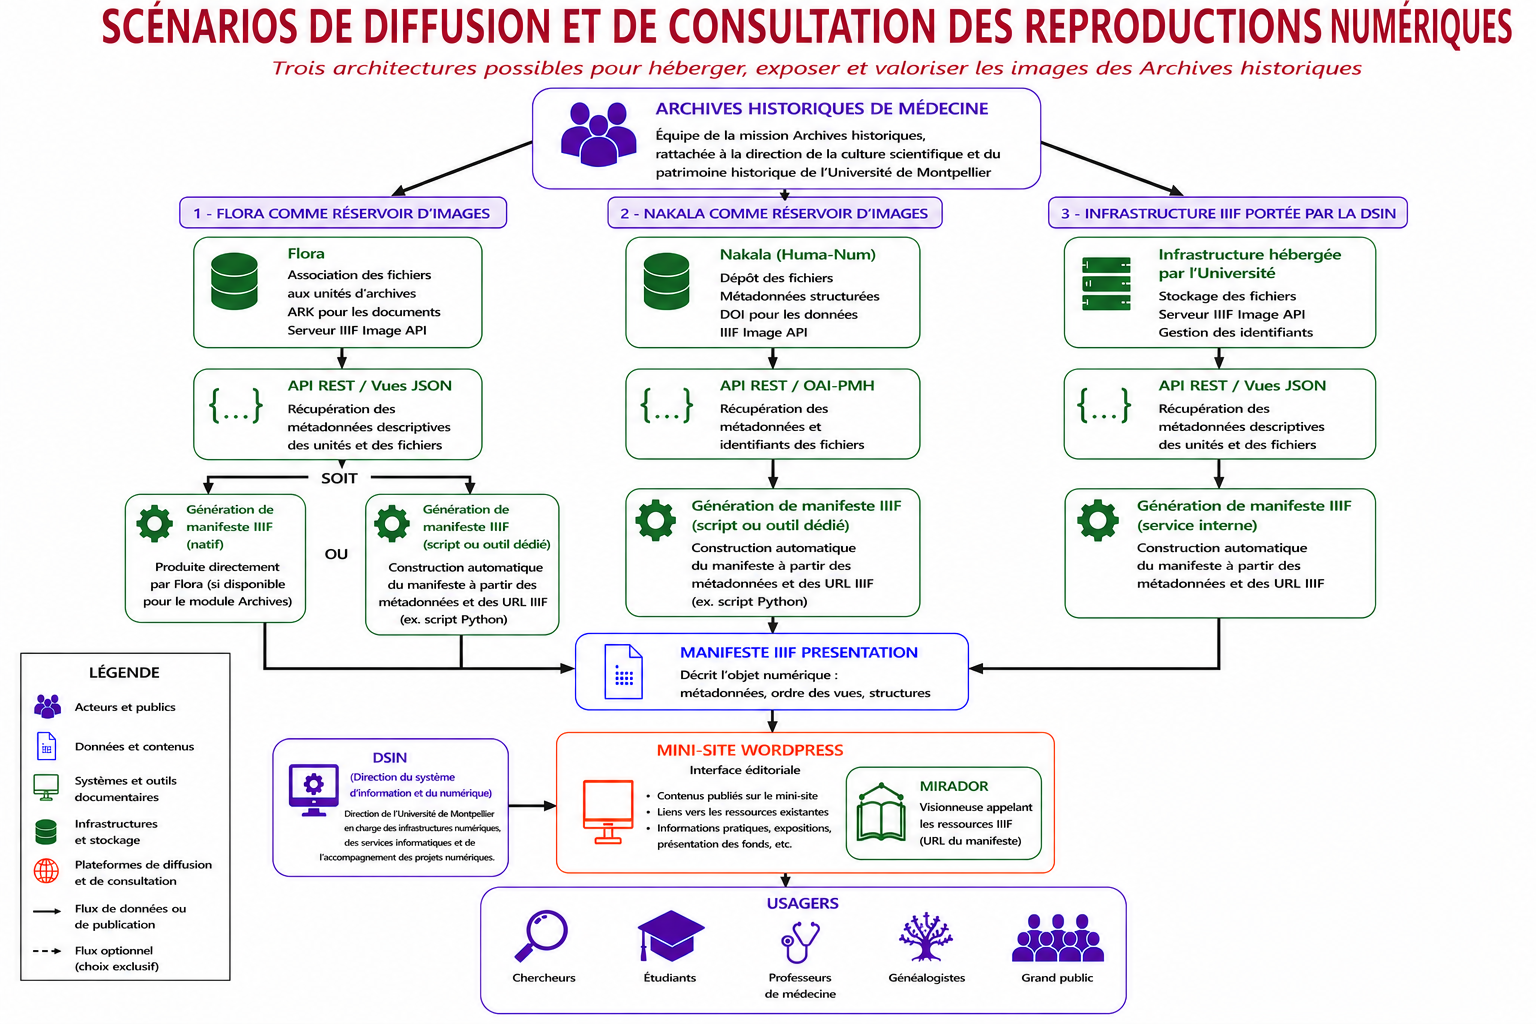
\includegraphics[
				width=\linewidth,
				height=1\textheight,
				keepaspectratio
				]{images/scenario2.png}
				\captionof{figure}{Scénarios envisagés pour l'hébergement, l'exposition et la consultation des reproductions numériques des Archives historiques}
				\label{fig:scenarios-diffusion-numerique}
			\end{minipage}%
		}
	\end{figure}
\end{landscape}

\chapter{Diffusion des archives historiques et gestion archivistique à l'échelle de l'Université}
\label{chap:systemes-information-archivistiques}
\chapitrecourt{Diffusion et gestion archivistique}

Les solutions examinées jusqu'ici répondent aux besoins immédiats de la Mission Archives historiques : produire et signaler les instruments de recherche, présenter les fonds, héberger les reproductions et en permettre la consultation. Leur articulation forme une architecture distribuée adaptée à un projet de diffusion, mais ne couvre pas l'ensemble des opérations archivistiques conduites à l'échelle de l'Université.

Le recours à un système d'information archivistique (\gls{sia}) relève d'une autre perspective : il vise à organiser dans un environnement métier commun la collecte, le traitement, la conservation et la communication des archives de l'établissement. Son étude conduit donc à changer d'échelle, depuis les dispositifs mobilisables par la Mission pour ses fonds historiques jusqu'à l'organisation de la fonction archives au niveau universitaire.


\section{Le \gls{sia} dans la gestion du cycle de vie des archives}
\label{sec:sia-changement-echelle}

\subsection{Les fonctions du \gls{sia}, de la collecte à la conservation définitive}

\paragraph{Un environnement commun pour les opérations archivistiques}

À la différence d'un \gls{cms}, d'un catalogue ou d'un portail documentaire, un \gls{sia} intervient dans les opérations quotidiennes du service. Selon son périmètre fonctionnel, il réunit la gestion des producteurs et des services versants, la collecte, les versements et les éliminations, le classement et la description, les localisations et le récolement, la communicabilité, les communications ainsi que la production d'instruments de recherche\footcite{Hamard2020}\footcite{MoalicMinnaert2023}.

Pour les archives courantes et intermédiaires, il assure principalement le suivi des producteurs et des versements, la localisation des articles, le contrôle des échéances, les éliminations et les communications. Pour les documents conservés définitivement, il prend en charge le classement hiérarchique, la description normalisée, la production des instruments de recherche et leur diffusion ou leur export.

\paragraph{La continuité des données au cours du cycle de vie}

L'intérêt du dispositif tient à la continuité des données entre ces différentes étapes. À l'issue de la durée d'utilité administrative, les documents éliminés sont retirés du système ; ceux qui doivent être conservés définitivement sont repris avec les informations déjà constituées sur leur producteur, leur provenance, leur versement, leur localisation et les traitements antérieurs. Le classement définitif complète ces données au lieu d'en imposer la reconstitution.

Cette continuité repose sur la constitution d'un \gls{referentiel} capable d'accompagner les documents au cours de leur cycle de vie. Elle prolonge l'évolution de l'informatisation archivistique, qui a progressivement étendu l'intervention de l'archiviste du traitement rétrospectif des fonds à la gestion des documents dès leur production\footcite{Hamard2020}.


\subsection{La séparation entre gestion métier et diffusion publique}

\paragraph{Des accès différenciés selon les utilisateurs et la communicabilité}

La continuité du traitement n'impose pas l'unicité des interfaces. Les solutions étudiées distinguent généralement un environnement professionnel de gestion d'une couche publique de diffusion : Mnesys Archives et Mnesys Expo, Ligéo Gestion et Ligéo Diffusion, ou encore Arkothèque Gestion et Arkothèque\footcite{MnesysLogiciels}\footcite{LigeoPresentation}\footcite{ArkothequePresentation}.

Cette séparation permet d'adapter les accès aux différents profils. Archivistes, services versants, agents de l'établissement et lecteurs extérieurs ne consultent pas les mêmes informations et n'accomplissent pas les mêmes opérations. Les habilitations doivent être articulées aux règles de communicabilité, aux restrictions particulières, aux éventuelles dérogations et aux conditions matérielles de consultation ; elles ne peuvent être réduites à une opposition entre contenus publiés et non publiés. Certaines solutions proposent ainsi des espaces distincts pour la collecte, le suivi des demandes et la gestion des communications\footcite{ArkothequeCollecte}\footcite{ArkothequeCommunication}.

Ces fonctions constituent l'un des points sur lesquels un \gls{sia} se distingue d'un logiciel documentaire plus généraliste. Les essais conduits par Sorbonne Université dans Flora ont ainsi révélé des difficultés à paramétrer assez finement les droits des administrateurs et des lecteurs et à traduire les règles de communicabilité dans l'interface de diffusion\footnote{Entretien avec Océane Valencia, responsable du Service des archives et du recueil des actes, Sorbonne Université, 6 juillet 2026.}. Sans remettre en cause les autres fonctions du logiciel, ce retour d'expérience montre les limites que peut rencontrer un outil qui n'est pas conçu prioritairement autour de la gestion du cycle de vie des archives. Dans un \gls{sia}, la communicabilité, les habilitations et les communications sont intégrées au traitement des unités documentaires et déterminent les conditions dans lesquelles celles-ci peuvent être rendues accessibles.

\paragraph{Le devenir du site éditorial selon le périmètre du \gls{sia}}

La présence d'un portail archivistique ne rend pas nécessairement inutile un site éditorial. Aux Archives municipales et métropolitaines de Montpellier, la base alimentée par Avenio donne accès depuis 2016 aux descriptions et aux ressources, tandis que le site créé en 2023 présente le service, ses activités et ses contenus de valorisation. Malgré leur rapprochement graphique, l'usager distingue encore difficilement le site institutionnel de la base ouverte par le bouton \enquote{Archives en ligne}\footnote{Entretien avec Claire Garcia, directrice adjointe et responsable de l'Unité Communication et Valorisation des Archives municipales et métropolitaines de Montpellier, 10 avril 2026.}. La coexistence de plusieurs interfaces suppose donc que leurs fonctions respectives soient clairement identifiables et que le parcours de l'une à l'autre demeure explicite.

À l'Université de Montpellier, la place du mini-site WordPress dépendrait ainsi du périmètre retenu pour un éventuel \gls{sia}. Limité à la gestion métier, celui-ci laisserait au mini-site ses fonctions de présentation de la Mission, d'information sur les modalités de consultation et de valorisation. L'acquisition d'une composante publique capable d'assurer à la fois la diffusion des instruments de recherche et des reproductions et l'accueil de contenus éditorialisés conduirait en revanche à réexaminer son maintien, afin d'éviter la duplication des informations et la multiplication des points d'accès.


\subsection{Le périmètre du \gls{sia} au regard des besoins et des moyens}

\paragraph{Des modules ajustés aux fonctions nécessaires}

Les solutions examinées pendant le stage --- principalement Mnesys, Ligéo, Avenio et Arkothèque --- organisent différemment la gestion, la diffusion et les échanges de données. Leur pertinence dépend des processus à prendre en charge, du volume et de l'état des données, du nombre d'utilisateurs, des habilitations nécessaires et des dispositifs de diffusion déjà en place.

Les retours d'expérience recueillis montrent que les établissements ne déploient pas nécessairement l'ensemble des composantes proposées. Après avoir comparé Flora, Mnesys, Ligéo, Avenio et Arkothèque, Sorbonne Université a retenu le seul module de gestion de Mnesys. Le portail n'a pas été acquis, les instruments de recherche étant déjà diffusés dans Calames et FranceArchives : le \gls{sia} est ainsi employé comme environnement métier, tandis que le \gls{signalement} et la consultation reposent sur des dispositifs extérieurs\footnote{Entretien avec Océane Valencia, responsable du Service des archives et du recueil des actes, Sorbonne Université, 6 juillet 2026.}.

À l'INALCO, deux ETP gèrent depuis 2025 environ 800 mètres linéaires avec Ligéo Gestion, principalement pour la collecte, les éliminations et les communications. Ligéo Diffusion n'a pas été acquis et les instruments restent proposés en PDF sur le site institutionnel ; Sciences Po utilise au contraire les deux composantes\footnote{Entretien avec Sarah Cadorel et Emma Bahous, INALCO, 15 juillet 2026.}\footcite{LigeoPresentation}. Arkothèque distingue pareillement la gestion des producteurs, des collectes, des versements, des éliminations et des communications de la publication des instruments et des ressources numériques\footcite{ArkothequeCollecte}\footcite{ArkothequeCommunication}\footcite{ArkothequePublication}. Ces configurations permettent d'ajuster le périmètre de l'outil métier aux besoins du service et aux dispositifs dont dispose déjà l'établissement.

Avenio offre une organisation différente. Aux Archives municipales et métropolitaines de Montpellier, les données métier alimentent directement la base publique et sa visionneuse\footnote{Entretien avec Claire Garcia, directrice adjointe et responsable de l'Unité Communication et Valorisation des Archives municipales et métropolitaines de Montpellier, 10 avril 2026.}. Cette comparaison reste indicative, l'échelle et les missions d'un service territorial différant de celles d'un établissement universitaire, mais elle confirme que l'articulation entre gestion et diffusion dépend du périmètre fonctionnel retenu plutôt que de l'existence d'un modèle unique de \gls{sia}.

\paragraph{Reprise des données, paramétrage et réorganisation du travail}

Le déploiement d'un \gls{sia} représente un investissement important. À Sorbonne Université, les quatre agents du service travaillaient depuis plusieurs mois à la préparation de Mnesys et avaient temporairement suspendu certaines opérations de collecte et de conseil afin de nettoyer et de restructurer les données\footnote{Entretien avec Océane Valencia, responsable du Service des archives et du recueil des actes, Sorbonne Université, 6 juillet 2026.}. À l'Université Paris Cité, la mise en œuvre, la migration et la formation auraient représenté environ une année de travail\footnote{Retour d'expérience de l'Université Paris Cité rapporté par Océane Valencia lors de l'entretien du 6 juillet 2026.}. Bien qu'indirect, ce retour fournit un ordre de grandeur de l'investissement organisationnel associé à une réinformatisation.

Une étude préalable devrait donc associer les futurs utilisateurs afin de formaliser les producteurs concernés, les procédures de collecte et de traitement, les données à reprendre, les règles de communicabilité, les habilitations, les échanges avec les autres applications et les besoins de diffusion. Le paramétrage ne se limite pas à transposer des pratiques existantes dans un logiciel : il les formalise et peut conduire à en reconfigurer certaines\footcite{MoalicMinnaert2023}.


\section{Une trajectoire de mise en œuvre pour les Archives historiques}
\label{sec:trajectoire-progressive}

L'étude des différents dispositifs permet de distinguer les opérations qui peuvent être engagées avec les moyens et les infrastructures actuellement disponibles de celles qui restent subordonnées à des choix techniques ou institutionnels. Le tableau~\ref{tab:comparaison-scenarios} rassemble les fonctions, les apports et les principales conditions de mise en œuvre des solutions examinées.

\begin{table}[htbp]
	\centering
	\tiny
	\setlength{\tabcolsep}{2pt}
	\renewcommand{\arraystretch}{1.15}
	\begin{tabularx}{\textwidth}{
			>{\raggedright\arraybackslash}p{1.75cm}
			>{\raggedright\arraybackslash}p{1.8cm}
			>{\raggedright\arraybackslash}p{2.15cm}
			>{\raggedright\arraybackslash}p{1.9cm}
			>{\raggedright\arraybackslash}X
			>{\raggedright\arraybackslash}X
		}
		\toprule
		\textbf{Dispositif} &
		\textbf{Fonction} &
		\textbf{Standards / échanges} &
		\textbf{Situation à l'UM} &
		\textbf{Intérêt} &
		\textbf{Conditions / limites} \\
		\midrule
		
		WordPress + \gls{mirador}
		& Médiation ; consultation des numérisations
		& \gls{iiif} Presentation
		& Mini-site déjà prototypé ; \gls{mirador} à intégrer
		& Interface éditoriale propre aux Archives ; réutilisation de ressources \gls{iiif} externes
		& Ne gère ni les descriptions archivistiques ni le stockage massif ; intégration de \gls{mirador} à réaliser \\
		
		\addlinespace
		
		SimplEAD + FranceArchives
		& \Gls{retroconversion} ; \gls{signalement} national
		& \gls{ead} 2002 ; \gls{oaipmh} côté FranceArchives
		& SimplEAD testé sur plusieurs instruments
		& Solution légère ; production d'un \gls{ead} valide sans déploiement d'un \gls{sia}
		& Sources maintenues localement ; nouvelle conversion après chaque modification ; identifiant du service à obtenir \\
		
		\addlinespace
		
		Calames
		& Production, maintenance et \gls{signalement} des instruments
		& \gls{ead} ; IdRef ; \gls{oaipmh}
		& Réseau déjà présent à l'UM
		& Production directe en \gls{ead} ; autorités partagées ; visibilité dans l'\gls{esr} et réutilisation des données
		& Intégration de la Mission à définir avec la référente et l'\Gls{abes} ; nouveaux déploiements suspendus pendant la refonte de Calames \\
		
		\addlinespace
		
		Flora
		& Gestion documentaire ; réservoir potentiel des reproductions
		& \gls{ark} ; \gls{api} \gls{json} ; \gls{iiif} Image
		& Déjà acquis et hébergé ; module Archives en cours de déploiement
		& Réutilisation d'une infrastructure institutionnelle ; absence d'un nouvel entrepôt
		& Export \gls{ead} testé non directement exploitable ; chaîne multi-images et \gls{iiif} Presentation non éprouvée \\
		
		\addlinespace
		
		Nakala
		& Hébergement et exposition des reproductions
		& \gls{doi} ; \gls{api} \gls{rest} ; \gls{oaipmh} ; \gls{iiif} Image
		& Non employé par la Mission
		& Entrepôt national indépendant des interfaces ; précédent Biblissima+ pour une chaîne \gls{iiif}
		& Nouvelle brique documentaire ; organisation des dépôts à définir ; \glspl{manifeste-iiif} Presentation à générer séparément \\
		
		\addlinespace
		
		Infrastructure \gls{dsin}
		& Hébergement ; services \gls{iiif} ; production des \glspl{manifeste-iiif}
		& \gls{iiif} Image / Presentation
		& Faisabilité évoquée ; architecture non définie
		& Maîtrise institutionnelle de la chaîne
		& Stockage, développement, sécurité et maintenance à dimensionner ; moyens non identifiés \\
		
		\addlinespace
		
		\gls{sia}
		& Gestion métier du cycle de vie
		& \gls{ead} et autres échanges selon la solution
		& Hypothèse à l'échelle de l'Université
		& Continuité des données entre archives courantes, intermédiaires et définitives
		& Projet institutionnel distinct : analyse des besoins, reprise des données, droits, paramétrage, formation et maintenance \\
		
		\bottomrule
	\end{tabularx}
	\caption{Fonctions, apports et conditions de mise en œuvre des dispositifs étudiés}
	\label{tab:comparaison-scenarios}
\end{table}


\subsection{Engager les opérations indépendantes des arbitrages techniques}

Plusieurs conditions demeurent ouvertes : l'identifiant nécessaire au versement dans FranceArchives, les modalités d'intégration à Calames, le devenir de cet environnement dans le cadre de sa refonte et le fonctionnement de la chaîne Flora--\gls{mirador}. Elles n'empêchent pas d'engager les travaux portant directement sur les données et les contenus.

Les instruments peuvent être harmonisés et repris progressivement ; ceux qui sont stabilisés peuvent être préparés dans SimplEAD ; la demande d'identification institutionnelle peut être adressée au \gls{siaf} ; les contenus et l'arborescence du mini-site peuvent être consolidés. La normalisation des producteurs, des cotes, des niveaux de description, des règles de communicabilité et des autorités prépare également leur utilisation dans des environnements ultérieurs. Le recours à l'\gls{ead} et à des \glspl{identifiant-perenne} permet de préserver leur capacité de circulation indépendamment de l'outil qui assure leur production ou leur publication à un moment donné.

Cette préparation intervient également dans la perspective d'une migration. Le passage des instruments de recherche de Harvard vers ArchivesSpace en fournit un exemple à une échelle beaucoup plus importante. Plus de 6\,000 instruments en \gls{ead}, représentant environ deux millions de composants archivistiques et issus de près de vingt années de pratiques d'encodage, devaient être repris dans le nouveau système. Malgré leur structuration dans un format commun, leurs variations internes et certaines données incompatibles avec le modèle cible auraient empêché l'import d'une part importante du corpus sans traitement préalable. La migration a reposé sur l'analyse des fichiers existants, l'identification de plusieurs dizaines de catégories de problèmes, leur transformation automatisée, puis des imports successifs dans un environnement de test contrôlés par les archivistes\footcite{MayoBowers2017}. Un format normalisé facilite donc la circulation des descriptions sans effacer l'hétérogénéité accumulée dans leurs modalités de production. L'harmonisation des instruments montpelliérains et la documentation des choix de structuration constituent à ce titre un travail préalable à leur exploitation présente comme à leurs éventuelles migrations futures.

Ces opérations doivent rester proportionnées aux priorités de la Mission, assurée par Sophie Dikoff et Emma Bertrand, et au calendrier de la demande de dérogation envisagée pour 2029. La connaissance et le classement des fonds, la révision ou la production des instruments de recherche, l'amélioration des conditions de conservation, l'organisation du service et la préparation du dossier demeurent prioritaires. Le développement de la diffusion numérique doit accompagner ces travaux sans mobiliser des moyens disproportionnés au regard des capacités actuelles du service.


\subsection{Éprouver les solutions disponibles avant de déployer de nouvelles infrastructures}

À court terme, SimplEAD permet de préparer le \gls{signalement} des instruments achevés, tandis que le mini-site assure leur médiation éditoriale. Pour les reproductions, Flora doit être testé en priorité puisque le logiciel est déjà acquis et en cours de déploiement à l'Université. L'essai devra vérifier la stabilité des identifiants et des URL, l'exposition des fichiers par \gls{iiif}, la production ou la génération extérieure des \glspl{manifeste-iiif} et leur restitution dans \gls{mirador}. Le recours à Nakala se justifierait si cette chaîne ne répond pas au besoin ; une infrastructure portée par la \gls{dsin} supposerait au préalable d'évaluer la charge de développement et de maintenance.

À moyen terme, Calames pourra être réexaminé avec la référente montpelliéraine et l'\Gls{abes}, lorsque les conditions d'intégration de la Mission et le calendrier de la refonte auront été précisés. Cette solution permettrait de remplacer la conversion ponctuelle des fichiers par une production et une maintenance partagées des instruments en \gls{ead}. Le projet Orion, qui renouvelle parallèlement le système de gestion des \glspl{metadonnees} et les outils de production de l'\Gls{abes}, devra également être suivi en raison de ses effets possibles sur l'écosystème documentaire de l'enseignement supérieur.

L'étude d'un \gls{sia} intervient à un horizon différent. Les retours d'expérience précédemment examinés montrent l'ampleur du travail de définition des processus, de reprise des données et de paramétrage qu'implique son déploiement. Son étude relève donc d'un projet institutionnel associant les différents acteurs de la fonction archives à l'échelle de l'Université, distinct des opérations de diffusion que la Mission peut engager à court et moyen terme.


\section*{Conclusion du chapitre et de la deuxième partie}
\phantomsection
\label{sec:conclusion-partie-ii}

L'étude, initialement centrée sur la création d'un portail propre aux Archives historiques, a conduit à dissocier plusieurs fonctions que la mise en ligne tendait d'abord à réunir : la médiation éditoriale, la production et le \gls{signalement} des descriptions, l'hébergement des reproductions et leur consultation. Les expérimentations menées montrent que leur prise en charge par des composants distincts permet de faire évoluer les dispositifs de diffusion sans imposer la reprise de l'ensemble des données. L'\gls{ead}, les \glspl{identifiant-perenne} et \gls{iiif} assurent à cet égard la circulation des descriptions et des reproductions entre des environnements susceptibles d'évoluer séparément.

Cette architecture distingue également deux échelles d'intervention. La Mission peut engager progressivement le \gls{signalement}, la médiation et la diffusion numérique de ses fonds à partir des infrastructures disponibles, tandis que la continuité de leur gestion avec celle des archives courantes et intermédiaires relève d'un éventuel \gls{sia} conçu à l'échelle de l'établissement. Les travaux entrepris sur les fonds historiques répondent ainsi aux besoins présents sans présumer de l'environnement métier qui pourrait être retenu ultérieurement.

La circulation des descriptions et des reproductions ouvre enfin la possibilité de rapprocher les Archives historiques des autres ensembles documentaires auxquels leur histoire les relie. Les personnes, institutions, enseignements et pratiques documentés par les fonds ont laissé d'autres traces dans les bibliothèques et les collections scientifiques de l'Université, comme dans les établissements patrimoniaux montpelliérains ; les données produites à partir des archives peuvent également rejoindre des réseaux documentaires et des infrastructures de recherche dépassant l'échelle locale. Ces relations entre collections, institutions et données constituent dès lors le prolongement de la réflexion sur leur diffusion.
	
	% Troisième partie
	\part{Perspectives d'inscription des archives historiques dans l'écosystème patrimonial et scientifique de l'enseignement supérieur}
\label{part:ecosysteme-patrimonial}

Les relations entre collections, institutions et données prennent des formes différentes selon l'échelle à laquelle les archives historiques sont envisagées. Au sein de l'Université de Montpellier, elles prennent place parmi des collections bibliographiques, muséales et scientifiques qui documentent parfois les mêmes personnes, institutions, enseignements ou pratiques, tout en relevant de traditions descriptives et d'environnements documentaires distincts. L'histoire de l'enseignement médical se reconstitue en outre à partir de sources aujourd'hui réparties entre plusieurs institutions de conservation et inscrites dans différents réseaux de \gls{signalement}. Enfin, certains ensembles documentaires peuvent être sélectionnés et transformés pour constituer des \glspl{corpus-numerique} répondant à une problématique de recherche déterminée.

La première échelle est donc celle du patrimoine universitaire. Elle conduit à examiner les rapprochements susceptibles d'être établis entre archives, collections bibliographiques et objets scientifiques à partir des entités qu'ils documentent en commun. L'\gls{interoperabilite} sémantique, les \glspl{referentiel} et la formalisation des relations permettent d'envisager ces rapprochements sans uniformiser les modèles descriptifs propres à chaque type de collection.

Le changement d'échelle devient ensuite institutionnel. Les sources relatives à l'histoire de l'enseignement médical montpelliérain dépassent les limites de l'Université actuelle : leur \gls{signalement} dans des réseaux collectifs, l'identification partagée de certains de leurs acteurs et la constitution d'ensembles patrimoniaux interinstitutionnels permettent de restituer des continuités que la répartition matérielle des documents rend moins immédiatement perceptibles. À cette mise en relation des ressources succède enfin leur transformation en objets de recherche : transcription, encodage, \gls{extraction-entites}, \gls{fouille-textes} et publication des données construisent, à partir d'une sélection de sources, des \glspl{corpus-numerique} dont la structure dépend d'une question et d'une méthode scientifiques.

Cette partie suit ainsi un élargissement progressif, depuis les collections de l'Université jusqu'aux réseaux interinstitutionnels, puis des ressources patrimoniales aux données produites pour la recherche.

% ============================================================
% CHAPITRE 8
% ============================================================

\chapter{Les archives historiques dans le patrimoine de l'Université de Montpellier}
\chapitrecourt{Les archives historiques dans le patrimoine universitaire}

% ============================================================

\section{Des collections décrites dans des environnements distincts}

Les archives historiques ne constituent pas le seul ensemble patrimonial conservé et diffusé au sein de l'Université de Montpellier. Bibliothèques, collections muséales et patrimoine scientifique disposent de leurs propres dispositifs de description, de numérisation et de publication, développés selon des logiques et à des rythmes différents. Leur comparaison permet de replacer les solutions étudiées dans la partie précédente dans un environnement institutionnel plus large et d'examiner la manière dont ces différentes composantes du patrimoine universitaire sont aujourd'hui susceptibles d'être rapprochées.

\paragraph{Le patrimoine documentaire : une chaîne ancienne de conservation et de diffusion}

La Bibliothèque universitaire historique de médecine bénéficie d'une politique ancienne de conservation et de valorisation. Constituée pour l'essentiel au début du XIX\textsuperscript{e} siècle à partir des ouvrages sélectionnés par Gabriel Prunelle dans les dépôts littéraires issus des confiscations révolutionnaires, elle conserve environ cent mille imprimés antérieurs au XIX\textsuperscript{e} siècle et près de neuf cents manuscrits, dont les deux tiers sont médiévaux\footcite{Dulieu1981}\footcite{Lorblanchet2015}. Le musée Atger, formé d'environ mille dessins et cinq mille estampes donnés entre 1813 et 1832, prolonge cette conception humaniste de la formation médicale en associant sciences et arts\footcite{Lorblanchet2015}.

La visibilité de ces collections résulte d'opérations successives de conservation, de catalogage et de reproduction. Dès les années 1990, l'atelier de conservation et le service photographique assuraient le microfilmage de sécurité des manuscrits, la reproduction des dessins du musée Atger et la fourniture d'images aux chercheurs et aux éditeurs\footcite[42--43]{Nicq1996}. Le projet \emph{Cantor et musicus} associait déjà numérisation des manuscrits médiévaux, enrichissement du \gls{signalement} et élargissement de l'accès\footcite[39--44]{Vial2001}. Les réorganisations institutionnelles et les déplacements des fonds ont néanmoins fragmenté les sources relatives à leur constitution. Depuis les années 2000, l'évaluation du \gls{signalement}, l'inventaire matériel, les constats d'état et la poursuite des numérisations ont contribué à leur réappropriation patrimoniale\footcite{Denton2025}.

Cette histoire explique l'existence d'une chaîne d'accès structurée. Primo constitue l'interface publique de recherche des bibliothèques de l'Université ; les imprimés et fonds anciens sont également signalés dans le Sudoc, tandis que les manuscrits et archives conservés par la bibliothèque sont décrits dans Calames. Foli@ donne accès à une sélection de manuscrits médiévaux et d'imprimés anciens numérisés, auxquels renvoient, selon les documents, les notices des catalogues nationaux\footcite{UMServicesPatrimoine}\footcite{SCDIFolia}. En amont, les ateliers du \gls{scdi} assurent les opérations de conservation-restauration, de photographie et de numérisation nécessaires à cette diffusion\footcite{SCDI2022}. Le \gls{signalement}, la conservation matérielle et l'accès aux reproductions reposent ainsi sur plusieurs services et outils complémentaires.

\paragraph{Les collections muséales et scientifiques : une professionnalisation progressive}

Les collections muséales et scientifiques ont suivi une autre trajectoire. À l'ancienne Université Montpellier 2, leur gestion s'est professionnalisée avec le recrutement d'un premier conservateur en 2004 et la création d'un Service des collections, devenu Pôle patrimoine scientifique\footcite{Gomel2011}. Celui-ci a repris des ensembles jusque-là principalement suivis par les enseignants, chercheurs et personnels techniques\footcite{Gomel2011}.

L'inventaire associe description matérielle et scientifique, historique et photographies des objets\footcite[54--57]{BourgadeTheronAumasson2014}. Au Conservatoire d'anatomie, sa reprise doit notamment établir une numérotation stable malgré les lacunes des anciens registres\footcite{Wenger2025}. La présence de restes humains impose en outre des procédures particulières d'identification, de conservation et de présentation\footcite{Ducourau2016}. Numérisation, expositions, manifestations et actions pédagogiques donnent parallèlement accès à des collections dont certaines sont dépourvues d'espace permanent d'exposition\footcite[58--61]{BourgadeTheronAumasson2014}.

La protection au titre des monuments historiques a également soutenu leur connaissance et leur sauvegarde\footcite{Palouzie2011}. Les 5\,688 pièces du Conservatoire d'anatomie ont été classées avec leur mobilier, leurs registres, leurs planches et dessins anatomiques, leurs écorchés et leurs squelettes d'animaux\footcite{POPAnatomieMontpellier}. Leur description est accessible dans Palissy, base nationale du patrimoine mobilier du ministère de la Culture, aujourd'hui diffusée au sein de la Plateforme ouverte du patrimoine (POP). L'accueil des collections Delmas-Orfila-Rouvière et Spitzner provenant de l'Université Paris-Descartes a ensuite nécessité des moyens humains et des réserves supplémentaires, ainsi que la poursuite des inventaires, restaurations, prêts et expositions\footcite[p.~62--65]{Girard2014}\footcite{PalouzieDucourau2017}\footcite{DucourauPinail2021}..

Palissy n'en fournit cependant pas un catalogue exhaustif, puisque son périmètre dépend de la protection des objets. À l'échelle institutionnelle, l'Université déploie désormais Flora comme logiciel commun de gestion des collections muséales et scientifiques. Il doit centraliser notices, \glspl{referentiel} et images, puis permettre la publication d'une sélection dans un portail public\footnote{\emph{Présentation de l'offre Flora Software à l'Université de Montpellier}, audition de négociation, 18 juillet 2024 ; \emph{Réunion de lancement du projet}, Flora Software -- Université de Montpellier, 14 février 2025}.

\paragraph{Les archives universitaires : une reconnaissance institutionnelle plus récente}

La trajectoire institutionnelle des archives historiques doit être replacée dans celle des archives universitaires françaises, dont la prise en charge spécialisée s'est développée plus tardivement que celle d'autres composantes du patrimoine universitaire. En l'absence de services internes dédiés, leur sauvegarde a longtemps reposé sur les Archives nationales et départementales ainsi que, dans certains cas, sur des bibliothèques municipales ou universitaires\footcite{MadayMechine2011}. À une période de faible investissement des universités jusqu'aux années 1980 ont succédé une sensibilisation progressive durant la décennie suivante, puis la multiplication des services spécialisés à partir des années 2000 : trois des soixante-quinze universités recensées en disposaient en octobre 2006, contre vingt-deux à la fin de 2012\footcite{Mercier2014}.

Ce décalage a été caractérisé comme un \enquote{double déficit de légitimité}, au regard des autres patrimoines reconnus et par comparaison avec les universités étrangères\footcite{Hottin2008}. Il affecte également l'exploitation scientifique des fonds et contribue aux déséquilibres documentaires et historiographiques entre établissements parisiens et universités de province\footcite{Dubois2022}. Le cas montpelliérain s'inscrit dans cette chronologie générale tout en présentant la particularité, mise en évidence dans la première partie, d'une conservation ancienne des archives de la Faculté précédant largement la constitution de la Mission qui en assure aujourd'hui le traitement spécialisé.

\paragraph{La \gls{dcsph} : un cadre institutionnel transversal}

La fusion des universités Montpellier 1 et Montpellier 2 en 2015 a rapproché des compétences patrimoniales développées selon des orientations complémentaires : l'ancienne Montpellier 2 avait notamment structuré l'inventaire et le conditionnement des collections scientifiques ainsi que leurs relations avec l'enseignement et la recherche, tandis que Montpellier 1 avait développé la restauration et la valorisation de son patrimoine historique et de ses collections\footcite{UMSchemaDirecteurPatrimoine2025}. La création de la \gls{dcsph} dans ce contexte a réuni les fonctions de préservation du patrimoine historique et de médiation scientifique au sein d'une même direction.

Son organisation actuelle comprend cinq services, dont trois directement consacrés au patrimoine : le Service du patrimoine historique, chargé notamment de la conservation, de l'étude, de l'inventaire et de la valorisation des collections mobilières et scientifiques ; le Service des collections patrimoniales documentaires, créé en 2021, qui prend en charge les collections patrimoniales des bibliothèques universitaires ; et la Mission Archives historiques (voir annexe~\ref{annexe:dcSPH}, fig.~\ref{fig:dcSPH-2025})\footcite{UMSchemaDirecteurPatrimoine2025}. Cette organisation place ainsi dans un même cadre institutionnel les objets, les collections documentaires et les archives qui témoignent de l'histoire de l'Université.

Le \emph{Schéma directeur du patrimoine historique et des collections} de 2025 donne une portée plus large à ce rapprochement. Il rattache explicitement les collections universitaires à leurs fonctions historiques d'enseignement et de recherche et fait de la réactivation de ces liens l'un des enjeux de la politique patrimoniale de l'établissement. Dans le cas de la Faculté de médecine, cette approche est particulièrement nette : le bâtiment historique est présenté comme un point d'entrée dans l'histoire de l'enseignement médical à travers les archives, le patrimoine documentaire et les collections mobilières, réunis dans une même lecture historique\footcite{UMSchemaDirecteurPatrimoine2025}.

\paragraph{Le \gls{scdi} : des compétences mutualisées à l'échelle interuniversitaire}

À ce cadre interne à l'Université s'ajoute un dispositif de coopération entre établissements. Créé le 1\textsuperscript{er} janvier 2021 dans le prolongement de missions auparavant exercées par la Bibliothèque interuniversitaire puis réparties entre les services documentaires issus des recompositions universitaires montpelliéraines, le \gls{scdi} intervient pour les universités de Montpellier dans des domaines qui gagnent à demeurer mutualisés : informatique documentaire, patrimoine écrit et graphique, circulation des documents, coordination du Sudoc, ressources électroniques et coopération régionale ou nationale\footcite{LorblanchetArabesques111}\footcite{SCDI2022}.

Dans le domaine patrimonial, cette mutualisation repose notamment sur un atelier de conservation-restauration et un atelier de numérisation-photographie. Le premier assure évaluations sanitaires, constats d'état, dépoussiérage, conditionnement, conservation préventive et traitements de restauration ; le second réalise les prises de vue et la numérisation des documents patrimoniaux, le traitement des fichiers et leur préparation pour la diffusion\footcite{LorblanchetAteliers2024}. Leur articulation est particulièrement importante lorsqu'une reproduction suppose une préparation matérielle ou des conditions particulières de manipulation. Au cours du stage, le diagnostic de plusieurs parchemins destinés à la restauration a ainsi montré que les choix de numérisation et de diffusion ne peuvent être dissociés de l'état matériel des documents.

Le \gls{scdi} ne se substitue ni aux établissements propriétaires ni aux services responsables des collections sur lesquelles il intervient. Son intérêt pour les archives historiques tient précisément à cette répartition : la Mission conserve la connaissance archivistique et la responsabilité de ses fonds, tandis que certaines opérations spécialisées de conservation, de photographie, de numérisation ou de diffusion peuvent s'appuyer sur des compétences et des équipements déjà mutualisés. Quelques registres des archives historiques sont actuellement accessibles sous forme numérisée dans Foli@ ; à la date de rédaction de ce mémoire, il n'est toutefois pas prévu que les futures numérisations de la Mission soient diffusées par cette plateforme. La mutualisation des compétences et des équipements du \gls{scdi} ne préjuge donc pas de l'environnement retenu pour la mise à disposition des reproductions. Le fonctionnement du \gls{scdi} fournit ainsi, parallèlement à l'organisation patrimoniale portée par la \gls{dcsph}, un exemple concret d'une coopération qui ne suppose pas la centralisation matérielle ou documentaire des collections.

Archives, livres et objets apparaissent ainsi comme des traces complémentaires de l'histoire universitaire, susceptibles d'être mobilisées conjointement pour documenter les enseignements, les pratiques scientifiques et les acteurs qui les ont produits ou utilisés. Ce rapprochement institutionnel et intellectuel conduit à déplacer la question vers les données elles-mêmes : certaines de ces relations peuvent-elles être formalisées de manière à être retrouvées et exploitées au-delà des publications ou projets de médiation qui les reconstituent ponctuellement ?


% ============================================================

\section{La mise en relation des archives, des livres et des objets}

\subsection{L'\gls{interoperabilite} sémantique des collections}

\paragraph{D'un rapprochement éditorial à une mise en relation des données}

La possibilité de rapprocher des ressources conservées dans plusieurs ensembles apparaît déjà dans les pratiques de médiation des universités. La série consacrée à François Rabelais sur \emph{Ex Bibliotheca}, carnet du \gls{scdi} hébergé sur Hypothèses, construit ainsi une même enquête à partir de documents conservés aux archives historiques et à la bibliothèque universitaire historique de médecine\footcite{ExBibliotheca}. L'inscription de Rabelais en 1530 est documentée par le registre des matricules S~19 et par le \emph{Liber procuratorum} S~2 ; son doctorat de 1537 par le registre des actes S~5 ; son enseignement des \emph{Pronostics} d'Hippocrate par le registre des leçons S~4\footcite{LorblanchetRabelais1}\footcite{LorblanchetRabelais2}. Ces sources archivistiques sont rapprochées des œuvres et éditions conservées par la bibliothèque, parmi lesquelles l'édition de 1532 des textes d'Hippocrate et de Galien publiée par Rabelais ainsi que différentes éditions de ses œuvres littéraires\footcite{LorblanchetRabelais4}. Guillaume Rondelet peut de même être suivi d'une ressource à l'autre : condisciple et ami de Rabelais, il apparaît dans le \emph{Tiers Livre} sous la figure de Rondibilis, tandis que ses propres ouvrages sont conservés dans les collections bibliographiques\footcite{LorblanchetRabelais3}.

Le rapprochement repose ici sur le travail intellectuel qui identifie les personnes, les événements, les œuvres et les documents pertinents puis les réunit dans un même récit. Il fournit un exemple concret de relations déjà établies entre les collections sans être exprimées comme telles dans leurs données descriptives. Leur formalisation permettrait de rendre une partie de cette contextualisation exploitable indépendamment de la publication qui l'a produite.


\paragraph{Du Web de documents au Web de données}

Archives, bibliothèques, musées et collections scientifiques reposent sur des traditions descriptives différentes. Un instrument de recherche restitue la provenance et l'organisation hiérarchique d'un fonds ; un catalogue de bibliothèque décrit des ressources bibliographiques ; un inventaire muséal individualise les objets, leur matérialité, leur provenance et leur état. Dans le cas du patrimoine scientifique, ces différences documentaires se superposent à des statuts juridiques et à des usages eux-mêmes variables\footcite{Cornu2016}.

La publication de ces \glspl{metadonnees} sur le Web ne suffit pas à assurer leur \gls{interoperabilite}. Le \gls{web-semantique} vise à rendre les données et les relations qu'elles entretiennent interprétables par les machines. Les \glspl{donnees-liees}, ou \emph{Linked Data}, en constituent une mise en œuvre fondée sur l'identification, la publication et la connexion de données structurées sur le Web\footcite{BizerHeathBernersLee2009}. Les ressources sont identifiées par des \glspl{uri} accessibles par \gls{http} et peuvent être décrites au moyen de \gls{rdf} (\emph{Resource Description Framework}), modèle standardisé de représentation des données sous la forme de relations entre ressources. Ces relations permettent notamment de relier une ressource à d'autres entités identifiées dans le même jeu de données ou dans des jeux de données extérieurs. Le passage d'un Web de documents à un Web de données consiste ainsi à rendre identifiables et manipulables non seulement des pages ou des notices, mais les entités auxquelles elles se rapportent et les relations qui les unissent.

Cette évolution est particulièrement intéressante pour des collections décrites dans des systèmes différents. Une personne, une institution, un lieu, une œuvre ou un événement peuvent être représentés comme des entités distinctes des notices dans lesquelles ils apparaissent et servir de points de jonction entre plusieurs jeux de données. Les \glspl{referentiel} jouent alors un rôle important : ils stabilisent l'identification de certaines entités et permettent de rapprocher des données produites indépendamment. Dans les institutions patrimoniales, cette logique peut contribuer à mettre en relation archives, bibliothèques et musées sans imposer la fusion de leurs systèmes descriptifs\footcite{Marcondes2012LinkedData}.


\paragraph{Du modèle conceptuel au graphe \gls{rdf}}

Une telle mise en relation suppose d'abord de déterminer ce que l'on souhaite représenter. La modélisation conceptuelle distingue les classes d'entités pertinentes pour un domaine, leurs caractéristiques et les relations qu'elles peuvent entretenir. Une personne, une activité, une œuvre ou un document constituent ainsi des catégories différentes, dont les occurrences concrètes sont des instances. Pour représenter informatiquement un ensemble dans lequel l'analyse porte principalement sur les relations entre ces entités, une organisation sous la forme d'un graphe est particulièrement adaptée : les entités y constituent des nœuds reliés entre eux par les relations qu'elles entretiennent.

Le \gls{rdf}, ou \emph{Resource Description Framework}, fournit un modèle standardisé pour représenter ce graphe. L'information y est décomposée en \glspl{triplet-rdf} associant un sujet, un prédicat et un objet\footcite{W3CRDF11Concepts}. Le sujet est une ressource identifiée par une \gls{uri} ; le prédicat, également identifié par une \gls{uri}, exprime une propriété ou la nature d'une relation ; l'objet peut être une autre ressource identifiée par une \gls{uri} ou un littéral, par exemple un nom, une date ou une valeur numérique. Les \glspl{triplet-rdf} qui partagent les mêmes ressources forment progressivement un graphe.

Cette structure permet de représenter aussi bien les caractéristiques d'une entité que ses relations avec d'autres entités. Une propriété reliant une ressource à un littéral peut par exemple exprimer une date, tandis qu'une propriété reliant deux ressources établit une relation entre elles. Le rattachement d'une instance à une classe est lui-même exprimé en \gls{rdf} par la propriété \verb|rdf:type|. Les classes et les propriétés peuvent être définies dans des vocabulaires ou des \glspl{ontologie} afin que leur signification soit documentée et réutilisable au-delà du jeu de données qui les emploie.

Le dossier documentaire constitué autour de Rabelais permet d'en proposer une représentation volontairement simplifiée. Le doctorat du 22 mai 1537 et l'enseignement des \emph{Pronostics} d'Hippocrate sont documentés respectivement par le registre des actes S~5 et le registre des leçons S~4\footcite{LorblanchetRabelais2}. L'édition lyonnaise de 1532 conservée sous la cote J~346 rassemble notamment les \emph{Pronostics} parmi les textes d'Hippocrate et de Galien publiés par Rabelais à partir des textes qu'il avait commentés à Montpellier\footcite{LorblanchetRabelais4}. Les \emph{Pronostics} peuvent dès lors être représentés comme une entité commune à l'activité d'enseignement attestée par les archives et à la ressource bibliographique conservée par la bibliothèque.

Avant de recourir à un vocabulaire formel, ces relations peuvent être décomposées sous la forme sujet--prédicat--objet afin d'expliciter la structure logique des assertions :

\begin{table}[htbp]
	\centering
	\small
	\begin{tabular}{p{0.26\textwidth} p{0.27\textwidth} p{0.35\textwidth}}
		\toprule
		\textbf{Sujet} & \textbf{Prédicat} & \textbf{Objet} \\
		\midrule
		
		François Rabelais
		& obtient
		& Doctorat du 22 mai 1537 \\
		
		Doctorat du 22 mai 1537
		& est documenté par
		& S~5, fol.~33 \\
		
		François Rabelais
		& dispense
		& Enseignement des \emph{Pronostics} \\
		
		Enseignement des \emph{Pronostics}
		& est documenté par
		& S~4, fol.~36 \\
		
		Enseignement des \emph{Pronostics}
		& porte sur
		& \emph{Pronostics} d'Hippocrate \\
		
		François Rabelais
		& publie
		& \emph{Hippocratis ac Galeni libri aliquot} \\
		
		\emph{Hippocratis ac Galeni libri aliquot}
		& contient
		& \emph{Pronostics} d'Hippocrate \\
		
		\bottomrule
	\end{tabular}
	
	\caption[Décomposition de relations documentaires autour de François Rabelais]
	{Décomposition simplifiée de plusieurs relations documentaires autour de François Rabelais sous la forme sujet--prédicat--objet. Les prédicats sont employés ici en langage naturel pour expliciter la structure des assertions avant leur traduction dans un vocabulaire formel.}
	\label{tab:rabelais-triplets-rdf}
\end{table}

Le tableau~\ref{tab:rabelais-triplets-rdf} explicite la structure logique des assertions sans constituer encore un jeu de données \gls{rdf} publiable. Dans une représentation effective en \gls{rdf}, les ressources devraient être identifiées par des \glspl{uri} et les propriétés empruntées à des vocabulaires existants ou définies dans un modèle documenté.


\paragraph{Du graphe à sa sérialisation en Turtle}

Le \gls{rdf} ne doit pas être confondu avec une syntaxe particulière d'encodage : il définit un modèle de données en graphe, qui peut être écrit selon plusieurs syntaxes de sérialisation. Turtle en constitue une représentation textuelle conçue pour être relativement compacte et lisible par un humain\footcite{W3CTurtle2014}. Les préfixes y permettent d'abréger les \glspl{uri} répétées ; le point termine un ensemble d'assertions et le point-virgule permet d'associer plusieurs prédicats à un même sujet sans répéter son \gls{uri}.

Afin de montrer concrètement la forme que pourraient prendre les assertions précédentes, l'exemple suivant utilise l'espace de noms fictif \verb|https://example.org/um/|. Les \glspl{uri} ainsi formées n'existent pas dans les systèmes de l'Université de Montpellier et servent uniquement à illustrer la syntaxe Turtle ; elles ne préjugent donc d'aucune politique institutionnelle d'identification des ressources.

\begin{verbatim}
	@prefix ex:  <https://example.org/um/> .
	@prefix xsd: <http://www.w3.org/2001/XMLSchema#> .
	
	ex:Rabelais
	ex:obtient ex:Doctorat1537 ;
	ex:dispense ex:EnseignementPronostics ;
	ex:publie ex:J346 .
	
	ex:Doctorat1537
	ex:date "1537-05-22"^^xsd:date ;
	ex:estDocumentePar ex:S5_fol33 .
	
	ex:EnseignementPronostics
	ex:estDocumentePar ex:S4_fol36 ;
	ex:porteSur ex:PronosticsHippocrate .
	
	ex:J346
	ex:contient ex:PronosticsHippocrate .
\end{verbatim}

Le préfixe \verb|ex:| constitue ici une simple abréviation : \verb|ex:Rabelais| correspondrait par exemple à l'\gls{uri} fictive \verb|https://example.org/um/Rabelais|. La déclaration \verb|@prefix| évite ainsi de répéter l'adresse complète devant chaque ressource. L'exemple distingue également deux formes de propriétés. \verb|ex:date| relie une ressource à un littéral typé : l'indication \verb|xsd:date| précise que la chaîne \verb|1537-05-22| doit être interprétée comme une date. À l'inverse, \verb|ex:porteSur|, \verb|ex:contient| ou \verb|ex:estDocumentePar| relient deux ressources identifiées. L'identifiant fictif \verb|ex:PronosticsHippocrate| fonctionne ainsi comme un nœud partagé par plusieurs branches du graphe.

Cet exemple ne constitue pas un jeu de données publiable en l'état. Les prédicats \verb|ex:obtient|, \verb|ex:dispense|, \verb|ex:publie|, \verb|ex:porteSur| ou \verb|ex:estDocumentePar| ont été créés pour rendre immédiatement lisibles les relations observées dans le corpus et ne sont définis par aucun vocabulaire partagé. Une mise en œuvre effective demanderait de déterminer quelles entités disposent déjà d'identifiants dans des \glspl{referentiel} externes, d'attribuer des \glspl{uri} aux ressources locales devant être publiées, de procéder lorsque cela est pertinent à leur \gls{reconciliation} avec des \glspl{referentiel} existants et de remplacer ces prédicats démonstratifs par des propriétés dont la sémantique est formellement définie.


\paragraph{De l'expérimentation à une infrastructure institutionnelle}

À l'échelle de l'Université, une telle mise en œuvre supposerait d'abord la définition d'une politique institutionnelle d'identification. Un espace d'\glspl{uri} placé sous un domaine contrôlé durablement par l'établissement pourrait identifier les ressources qui ne disposent pas déjà d'un identifiant externe approprié : objets scientifiques, activités, documents ou autres entités locales selon le périmètre retenu. Cette politique devrait déterminer les catégories d'entités auxquelles l'Université attribue ses propres identifiants, leurs règles de construction, l'autorité responsable de leur attribution et les conditions de leur maintien dans le temps. Une \gls{uri} publiée ne devrait notamment pas être réattribuée à une autre ressource si celle qu'elle identifie disparaît d'une application. La stabilité de ces identifiants permettrait ainsi de dissocier l'identification des entités de l'évolution des logiciels dans lesquels leurs descriptions sont produites.

La constitution du graphe n'impliquerait pas de remplacer les systèmes documentaires existants ni de saisir une seconde fois l'ensemble de leurs données. Les descriptions continueraient à être produites dans les environnements adaptés aux différentes collections. Des traitements d'extraction sélectionneraient dans ces sources les informations nécessaires au graphe, par exemple au moyen d'un export ou d'une \gls{api} lorsque le système en propose une. Des traitements de transformation convertiraient ensuite leur structure et leurs valeurs vers les classes et propriétés retenues pour le modèle commun. À ces opérations pourrait s'ajouter l'\gls{alignement}, qui établit des correspondances entre les éléments de modèles ou de vocabulaires différents, ainsi que la \gls{reconciliation}, qui cherche à déterminer si plusieurs occurrences désignent une même entité. Un nom de personne provenant de plusieurs systèmes pourrait ainsi être rapproché d'une même autorité IdRef, tandis que les informations propres à chaque description resteraient administrées dans leur environnement d'origine.

Les \glspl{triplet-rdf} ainsi produits pourraient être conservés dans un \emph{triple store}, logiciel ou système de gestion de données spécialisé dans le stockage et l'interrogation de graphes \gls{rdf}. Il existe à cette fin des solutions libres susceptibles d'être déployées sur une infrastructure administrée par l'établissement, comme Apache Jena, dont le serveur Fuseki permet notamment l'exposition et l'interrogation de données \gls{rdf}, ainsi que des solutions commerciales ou des services hébergés. Le recours à un \emph{triple store} ne supposerait donc pas que l'Université développe elle-même un système de stockage. Celui-ci ne constituerait pas davantage un nouvel outil de catalogage pour les responsables des collections : il formerait une couche transversale alimentée à partir des différents systèmes documentaires et consacrée à la mise en relation de certaines de leurs données.

L'exploitation de cette couche pourrait reposer sur plusieurs modes d'accès. Une \gls{api} permet à une application d'interroger automatiquement un service et d'en récupérer les données selon des modalités définies, sans passer par une interface de consultation humaine. Un \emph{endpoint} \gls{sparql} offrirait un accès spécifiquement destiné à l'interrogation du graphe : \gls{sparql} est un langage de requête permettant de rechercher des motifs de relations dans des données \gls{rdf}, tandis que l'\emph{endpoint} constitue l'adresse du service auquel ces requêtes sont envoyées et qui en retourne les résultats. Une requête pourrait par exemple rechercher les personnes reliées à la fois à des ressources archivistiques et bibliographiques, ou les objets scientifiques associés à une activité ou à une personne également documentée par les archives. Un tel \emph{endpoint} ne devrait pas nécessairement être ouvert sans restriction au public : il pourrait être réservé à certains usages tandis qu'une \gls{api} ou des interfaces de consultation exposeraient des services plus encadrés.

Les \glspl{uri} publiées devraient enfin être résolvables sur le Web. L'accès à l'\gls{uri} d'une entité pourrait fournir une représentation adaptée à l'usage qui en est fait : une page lisible dans un navigateur pour la consultation humaine ou une représentation structurée, par exemple en Turtle ou en \gls{jsonld}, pour une application. L'\gls{uri} constituerait ainsi un point d'accès stable à l'entité indépendamment de la forme sous laquelle les informations qui la concernent sont restituées. Stockage du graphe dans un \emph{triple store}, interrogation par \gls{sparql}, exposition de services par une \gls{api} et résolution des \glspl{uri} correspondent dès lors à des fonctions distinctes, susceptibles d'être assurées par plusieurs composants techniques.

Appliquée à Montpellier, cette architecture ferait du graphe une couche de mise en relation plutôt qu'un système documentaire supplémentaire destiné à absorber les autres. Les archives historiques pourraient continuer à produire leurs descriptions archivistiques dans leur environnement propre, tandis que les données bibliographiques et celles relatives aux collections scientifiques resteraient administrées dans leurs systèmes respectifs. Des traitements automatisés pourraient extraire les informations nécessaires depuis ces différents environnements, les transformer selon le modèle commun et les rapprocher, lorsque cela est pertinent, de \glspl{referentiel} partagés. Seules les entités et les relations utiles aux rapprochements retenus alimenteraient ainsi le graphe \gls{rdf}.

La mise en œuvre d'un tel dispositif ne supposerait donc pas le développement intégral d'une nouvelle infrastructure par l'Université. Elle nécessiterait en revanche de définir une politique institutionnelle pour l'attribution et la pérennité des \glspl{uri}, de déterminer le modèle et les vocabulaires partagés, d'organiser les traitements d'extraction, de transformation, d'\gls{alignement} et de \gls{reconciliation}, puis d'attribuer les responsabilités relatives à l'hébergement, à l'alimentation et à la maintenance de cette couche commune. Sa pérennité dépendrait ainsi autant de cette gouvernance que des composants techniques retenus.

\paragraph{\Glspl{referentiel}, \gls{reconciliation} et \glspl{ontologie}}

L'identification commune des entités constitue l'une des conditions de la mise en relation de jeux de données distincts. Les \glspl{referentiel} de personnes, collectivités, lieux, œuvres ou concepts peuvent servir de points d'appui à cette identification : plutôt que de rapprocher des chaînes de caractères identiques ou voisines, la \gls{reconciliation} cherche à déterminer si les données renvoient effectivement à une même entité. Un identifiant partagé peut alors jouer un rôle de pivot entre plusieurs systèmes.

Le cas de Rabelais permet d'en préciser l'intérêt à Montpellier. Son nom apparaît dans les descriptions des documents conservés aux archives historiques, dans les notices bibliographiques des ouvrages conservés par la Bibliothèque universitaire historique de médecine et dans les contenus éditoriaux qui rapprochent aujourd'hui ces ressources. La reconnaissance de la chaîne de caractères « François Rabelais » dans plusieurs bases ne suffit cependant pas à établir informatiquement qu'elles désignent une même personne. Une opération de \gls{reconciliation} consisterait à rapprocher ces différentes occurrences d'une même entité identifiée dans un \gls{referentiel} de personnes. Les descriptions resteraient administrées dans leurs environnements respectifs, mais pourraient partager ou aligner l'identifiant correspondant à Rabelais et rendre ainsi explicite leur point commun.

La même méthode pourrait être appliquée à d'autres entités attestées dans plusieurs collections de l'Université. Une collectivité ayant produit des archives et publié des documents, un professeur apparaissant à la fois comme producteur d'un fonds et auteur d'ouvrages, ou une œuvre conservée sous plusieurs formes pourraient être rapprochés à condition d'établir qu'il s'agit effectivement de la même entité. Le travail préalable consisterait donc à repérer les entités communes, à examiner les informations permettant de les identifier et à rechercher leur éventuelle présence dans des \glspl{referentiel} existants. La \gls{reconciliation} ne créerait pas la relation historique entre les ressources : elle fournirait un moyen de rendre exploitable dans les données une identification préalablement établie.

Les relations établies entre \glspl{referentiel} doivent elles-mêmes être qualifiées. Une relation d'identité entre deux ressources n'a pas la même portée qu'une correspondance entre deux concepts appartenant à des thésaurus distincts. Dans le contexte montpelliérain, l'objectif ne serait donc pas de constituer immédiatement un \gls{referentiel} unique pour l'ensemble des collections, mais de déterminer quels identifiants existants peuvent servir de points de jonction et quelles entités nécessiteraient une identification locale. L'\gls{interoperabilite} sémantique peut ainsi s'appuyer sur des données administrées dans plusieurs systèmes sans imposer leur fusion.

Les \glspl{ontologie} interviennent à un autre niveau. Elles ne servent plus seulement à déterminer que deux données renvoient à une même entité, mais à définir la nature des entités et des relations qui les unissent. Les prédicats fictifs employés dans l'exemple Turtle précédent --- \verb|ex:publie|, \verb|ex:porteSur| ou \verb|ex:estDocumentePar| --- rendent immédiatement lisibles les relations observées dans le corpus Rabelais, mais leur sémantique n'est définie par aucun modèle partagé. Une propriété formellement définie peut au contraire préciser les classes susceptibles d'apparaître comme sujet et comme objet ainsi que le sens exact de la relation. Le passage des identifiants partagés à la formalisation de ces relations conduit ainsi à examiner les \glspl{ontologie} susceptibles de fournir un modèle commun aux différentes collections ; le \gls{cidoccrm} offre dans ce domaine un cadre particulièrement adapté au patrimoine culturel.


\paragraph{\gls{cidoccrm} comme modèle conceptuel commun}

Le \gls{cidoccrm} fournit précisément un cadre conceptuel pour représenter des informations patrimoniales hétérogènes. Issu des travaux du Comité international pour la documentation de l'ICOM et normalisé par ISO~21127, il définit un ensemble de classes et de propriétés destiné à faciliter l'intégration, la médiation et l'échange d'informations entre sources documentaires\footcite{CIDOCCRM713}. Son intérêt pour des collections hétérogènes tient notamment à une modélisation orientée vers les événements : les personnes, groupes, objets, documents, lieux et autres entités persistantes peuvent être reliés par les événements et activités auxquels ils participent.

Cette organisation diffère d'une description fondée principalement sur l'accumulation d'attributs attachés à une notice. Les informations sont exprimées à travers des instances de classes et les propriétés qui les relient ; chaque propriété possède un domaine et un co-domaine qui précisent les catégories d'entités entre lesquelles elle peut être employée. Une même activité peut ainsi être reliée à un acteur, à une temporalité, aux documents qui permettent de la connaître et aux ressources qu'elle mobilise, tandis qu'un objet matériel peut être distingué du contenu symbolique qu'il porte.

Le cas de Rabelais permet d'en éprouver concrètement le principe. Dans la proposition de modélisation présentée en annexe~\ref{annexe:rabelais-cidoccrm}, François Rabelais est représenté comme une instance de \emph{E21 Person}. La collation de son doctorat et son enseignement sont représentés comme des instances de \emph{E7 Activity}, tandis que leurs temporalités relèvent de \emph{E52 Time-Span}. Les propriétés \emph{P11 had participant}, \emph{P14 carried out by} et \emph{P4 has time-span} permettent respectivement de représenter la participation de Rabelais à la collation de son doctorat, son rôle dans l'activité d'enseignement et la temporalité de ces activités.

La modélisation conduit également à distinguer le support matériel d'archives de l'information documentaire qu'il porte. Le registre des actes S~5 et le registre des leçons S~4 sont considérés, dans leur matérialité, comme des instances de \emph{E22 Human-Made Object}. Les mentions du doctorat et de l'enseignement inscrites dans ces registres sont représentées comme des instances de \emph{E31 Document}. La propriété \emph{P128 carries} relie alors le support matériel au contenu documentaire qu'il porte, tandis que \emph{P70 documents} relie ce contenu à l'activité qu'il documente. Cette distinction évite de confondre le registre comme objet conservé avec l'information documentaire inscrite sur ce support.

Une distinction comparable est opérée pour la ressource bibliographique. L'exemplaire conservé sous la cote J~346 est représenté comme une instance de \emph{E22 Human-Made Object}, tandis que les \emph{Pronostics} d'Hippocrate relèvent de \emph{E33 Linguistic Object}. La propriété \emph{P128 carries} permet de relier l'exemplaire matériel au contenu linguistique qu'il porte. L'activité d'enseignement peut en outre être reliée aux \emph{Pronostics} par \emph{P16 used specific object}, propriété qui associe une activité à la ressource spécifique qu'elle mobilise. Le rapprochement initialement exprimé en langage naturel par « l'enseignement porte sur les \emph{Pronostics} » est ainsi reformulé au moyen d'une propriété dont la sémantique est définie dans le \gls{cidoccrm}.

Le passage du tableau~\ref{tab:rabelais-triplets-rdf} et de l'exemple Turtle au schéma présenté en annexe~\ref{annexe:rabelais-cidoccrm} montre ainsi la différence entre la structure d'un graphe et sa modélisation sémantique. Le \gls{rdf} permet d'exprimer des assertions sous la forme de \glspl{triplet-rdf}, mais n'impose pas à lui seul la signification de propriétés telles que « documente », « participe à » ou « porte ». Le recours au \gls{cidoccrm} contraint au contraire leur emploi par la définition des classes, des propriétés, de leurs domaines et de leurs co-domaines. La formalisation ne consiste donc pas à transformer mécaniquement les verbes d'une analyse documentaire en prédicats, mais à déterminer si les relations observées peuvent être exprimées par les concepts d'un modèle partagé.

La proposition demeure nécessairement partielle. Le choix des classes et des propriétés dépend du niveau de granularité retenu et des informations effectivement attestées par les sources ; une modélisation plus poussée pourrait notamment distinguer plus finement l'édition de 1532, l'exemplaire J~346 et les différents textes qu'il contient. Son intérêt réside ici dans la possibilité de remplacer certaines relations exprimées en langage courant par des relations dont la signification et les conditions d'emploi sont explicitement définies dans le \gls{cidoccrm}.

Une telle modélisation peut être construite à partir de descriptions existantes. Les \glspl{metadonnees} des Archives nationales portugaises ont ainsi fait l'objet d'une mise en correspondance d'éléments issus de \gls{isadg} avec les classes et propriétés du \gls{cidoccrm}. Cette transformation permet de conserver l'information archivistique tout en la rendant exploitable dans un modèle fondé sur des entités et des relations\footcite{MeloRodriguesVaragnolo2023}. La description hiérarchique du fonds conserve sa fonction archivistique, tandis qu'une représentation complémentaire autorise d'autres parcours à travers les personnes, les lieux, les événements ou les temporalités documentés.

Le Musée virtuel de l'Université de Barcelone fournit un point de comparaison particulièrement proche du contexte montpelliérain. Les collections scientifiques, artistiques et facultaires de l'établissement, auxquelles s'articulent les ressources patrimoniales de la bibliothèque et des archives, étaient initialement documentées dans plusieurs environnements ; leur rapprochement a conduit à rechercher une représentation transversale respectant la diversité de ces collections\footcite{SalseRoviraEtAl2024UniversityHeritage}. La solution retenue repose sur un \gls{profil-application} fondé sur \gls{dcmi} Metadata Terms, enrichi notamment par des éléments du \gls{cidoccrm} et de \gls{lido}, afin d'obtenir un niveau d'\gls{interoperabilite} compatible avec les moyens et les pratiques quotidiennes des responsables de collections\footcite{SalseRoviraMateoBretos2025DublinCore}.

L'expérience barcelonaise montre également que l'\gls{interoperabilite} dépend du travail effectué sur les données en amont de leur publication. Nettoyage, normalisation et \gls{reconciliation} permettent d'identifier plus sûrement les personnes, lieux et autres entités et de les rapprocher de \glspl{referentiel} externes. OpenRefine est notamment employé dans ce processus de préparation à l'enrichissement sémantique\footcite{SalseRoviraMateoBretos2025}. La \emph{Minimum Record Recommendation} poursuit une logique comparable en proposant aux petites collections un noyau descriptif réduit mis en correspondance avec le \gls{cidoccrm}, \gls{lido} et l'\gls{edm}\footcite{StadtlerStricker2024}.

À Montpellier, le corpus Rabelais fournit ainsi un premier ensemble suffisamment circonscrit pour éprouver cette démarche entre archives et collections bibliographiques. Les personnes, actes universitaires, activités d'enseignement, œuvres et éditions identifiés dans \emph{Ex Bibliotheca} permettent de tester la définition des classes utiles, le niveau de granularité des entités, la \gls{reconciliation} avec des \glspl{referentiel} existants et la sélection de propriétés correspondant réellement aux relations documentées. Une extension aux collections scientifiques devrait suivre la même méthode en partant de liens attestés entre documents et objets, plutôt que de rapprochements exclusivement nominaux ou thématiques. Le \emph{Schéma directeur du patrimoine historique et des collections}, qui considère conjointement les différentes traces de l'histoire de l'enseignement et de la recherche conservées par l'Université, fournit à cette approche un cadre institutionnel particulièrement favorable\footcite{UMSchemaDirecteurPatrimoine2025}.

% ============================================================

\subsection{Relier les archives aux collections scientifiques : l'apport de \gls{patstec}}

\paragraph{Documenter l'objet scientifique par ses sources}

Créée en 2003 par le ministère chargé de la Recherche et coordonnée par le Musée des Arts et Métiers, la Mission nationale de sauvegarde du patrimoine scientifique et technique contemporain, dite \gls{patstec}, anime un réseau d'universités, d'organismes de recherche, de musées et d'entreprises. Sa base nationale documente les instruments de recherche, d'enseignement et d'innovation et peut leur associer vidéos, témoignages, parcours de chercheurs, cahiers de laboratoire et autres ressources éclairant leur fonctionnement et leurs usages\footcite{PATSTECMission}.

Cette méthode présente un intérêt particulier pour les archives universitaires parce qu'elle envisage l'objet scientifique à partir de l'ensemble documentaire qui permet d'en restituer l'histoire. Les archives peuvent renseigner sa conception, son acquisition, ses transformations et son utilisation dans un laboratoire ou un enseignement, tandis que l'objet conserve la matérialité d'une pratique scientifique dont les dossiers fournissent d'autres traces\footcite{Joyaux2018}. La relation entre les deux ressources repose ainsi sur l'identification de l'instrument, des acteurs et des activités auxquels les documents se rapportent.

\gls{patstec} fournit de ce point de vue une réalisation concrète de la logique examinée précédemment : la notice d'un instrument peut être enrichie par des ressources complémentaires, notamment des témoignages, cahiers de laboratoire, photographies ou documents techniques qui en renseignent le fonctionnement et le contexte scientifique. La documentation de l'objet peut ainsi restituer les activités de recherche et d'enseignement auxquelles il a participé et les acteurs qui l'ont conçu, employé ou transformé.

\paragraph{Un cas montpelliérain : Émile Jeanbrau et la transfusion sanguine}

L'Université de Montpellier porte la mission \gls{patstec} Occitanie-Est\footcite{PATSTECOccitanieEst}. Le sous-fonds Émile Jeanbrau relatif à la transfusion sanguine fournit un exemple particulièrement précis de relation entre un objet scientifique et les archives qui permettent d'en restituer l'usage. Son instrument de recherche signale un appareil conservé au Conservatoire d'anatomie, tandis que plusieurs dossiers documentent les techniques de transfusion, les instruments employés, l'usage du sang citraté, des photographies réalisées en 1917 et des schémas de l'appareil\footcite[notamment 1EJ55, 1EJ59, 1EJ87, 1EJ91--96, 1EJ105, 1EJ107, 1EJ110 et 1EJ144]{BertrandDikoff2024Jeanbrau}.

L'appareil n'est pas identifiable dans la base publique de \gls{patstec} et sa datation excède le périmètre chronologique affiché par le programme national\footcite{PATSTECObjets}. Le cas permet en revanche d'envisager une transposition locale de la méthode : la notice de l'objet pourrait renvoyer vers les dossiers qui renseignent sa conception, ses caractéristiques ou ses usages, tandis que l'instrument de recherche pourrait identifier explicitement l'objet conservé au Conservatoire d'anatomie. Émile Jeanbrau, l'appareil, les activités de transfusion, les documents techniques, les photographies et les schémas formeraient ainsi un ensemble de ressources dont les relations peuvent être établies à partir des sources.

Le rapprochement diffère du cas Rabelais par la nature des ressources mises en relation. Autour de Rabelais, les relations associent principalement des activités universitaires, des actes d'archives, des œuvres et des ressources bibliographiques ; autour de Jeanbrau, elles relient un acteur, une pratique médicale, un instrument scientifique et les documents qui en renseignent l'histoire. Le principe documentaire reste identique : une relation transversale devient exploitable lorsqu'elle porte sur des entités suffisamment précisément identifiées et repose sur des sources qui permettent d'en qualifier la nature.


% ============================================================
% CHAPITRE 9
% ============================================================

% ============================================================
% CHAPITRE 9
% ============================================================

\chapter{Les archives historiques dans les réseaux et corpus interinstitutionnels}
\chapitrecourt{Réseaux et corpus interinstitutionnels}

% ============================================================

Le rapprochement des collections de l'Université constitue un premier niveau d'intégration. L'histoire de l'enseignement médical montpelliérain déborde cependant les limites de l'établissement : les documents qui permettent de la retracer sont aujourd'hui conservés par plusieurs institutions et décrits dans plusieurs réseaux. Leur réunion matérielle n'est ni possible ni souhaitable ; leur mise en relation repose sur des dispositifs qui interviennent à des niveaux différents. Le \gls{signalement} collectif rend les fonds repérables depuis plusieurs environnements documentaires ; les \glspl{referentiel} permettent d'identifier certaines des personnes et collectivités qui les traversent ; la candidature au registre \emph{Mémoire du monde} construit l'unité patrimoniale d'un ensemble dispersé ; Biblissima+ permet enfin d'envisager, à partir de ressources sélectionnées, des \glspl{corpus-numerique} organisés selon leur transmission et leur exploitation scientifique.

Le changement d'échelle est donc à la fois institutionnel et documentaire. Il ne consiste plus seulement à diffuser les archives historiques hors de la Faculté, mais à les rendre susceptibles d'être découvertes, rapprochées et exploitées avec des ressources conservées ailleurs. Dans cette perspective, la conservation \emph{in situ} ne constitue pas un obstacle : ce sont les descriptions, les \glspl{identifiant-perenne}, les reproductions et les données produites à partir des fonds qui circulent entre les réseaux.


% ============================================================

\section{Le \gls{signalement} des fonds et l'identification de leurs acteurs}

\subsection{Calames et FranceArchives : deux réseaux de \gls{signalement}}

\paragraph{Deux constructions collectives issues de traditions documentaires différentes}

Calames et FranceArchives ne constituent pas deux interfaces équivalentes dans lesquelles une même description serait simplement reproduite. Leur histoire et leur périmètre expliquent les fonctions différentes qu'ils peuvent remplir pour les archives historiques.

Calames est issu de la constitution, au cours des années 2000, d'un environnement collectif consacré aux manuscrits et aux archives conservés dans l'enseignement supérieur. Sa création prolonge notamment la rétroconversion en \gls{ead} du \emph{Catalogue général des manuscrits} et du répertoire PALME : l'interface publique ouvre en décembre 2007, puis l'outil professionnel de catalogage partagé est déployé auprès d'un premier groupe d'établissements en 2008\footcite{AbesHistoireCalames}\footcite{NoelCalames2020}. Le réseau réunit désormais une soixantaine d'établissements de l'\gls{esr}, dans lesquels peuvent être signalés manuscrits médiévaux, archives scientifiques, fonds littéraires, iconographie ou papiers de chercheurs\footcite{AbesCatalogueCalames2026}. À la fin de 2023, sa base de production comptait plus de 1,74 million de composants \gls{ead} ; 56\,970 nouveaux composants avaient été publiés au cours de cette seule année et environ 78\,000 nouveaux liens entre descriptions et autorités  avaient été ajoutés\footcite{AbesCalamesStat2023}.

Cette volumétrie donne une portée différente au \gls{signalement} envisagé pour Montpellier. L'intégration des archives historiques ne consisterait pas seulement à disposer d'une nouvelle adresse publique pour leurs instruments de recherche : elle les placerait dans un catalogue où les unités archivistiques sont mises en relation avec des fonds de même nature produits ou conservés dans d'autres établissements de l'\gls{esr}. Une recherche portant sur un professeur, une discipline, une société savante ou une institution scientifique pourrait ainsi faire apparaître conjointement les ressources montpelliéraines et des archives universitaires ou scientifiques conservées ailleurs. La description hiérarchique continuerait de restituer la provenance et la structure propre de chaque fonds, tandis que les points d'accès et les \glspl{donnee-autorite} permettraient les rapprochements transversaux.

FranceArchives procède d'une autre logique. Ouvert en 2017, le portail national agrège les instruments de recherche de services relevant de réseaux beaucoup plus divers : Archives nationales, services ministériels, Archives départementales, municipales ou métropolitaines, établissements publics, associations et autres institutions conservant des archives. En mai 2026, 241 partenaires y participaient et 108\,504 inventaires y étaient intégrés ; le portail recevait en moyenne environ 300\,000 visiteurs uniques par mois\footcite{FranceArchivesRejoindre2026}. FranceArchives constitue également l'agrégateur national vers le Portail européen des archives, de sorte que le \gls{signalement} local peut s'inscrire dans une chaîne de découverte dépassant le seul cadre français\footcite{FranceArchivesRejoindre2026}.

\paragraph{Reconstituer un paysage documentaire montpelliérain sans réunir les fonds}

Cette différence de périmètre présente un intérêt particulier à Montpellier. L'histoire institutionnelle de l'ancienne Université de médecine a produit des archives aujourd'hui réparties entre la Faculté, les Archives départementales de l'Hérault et les Archives municipales de Montpellier. La dispersion résulte de trajectoires documentaires et institutionnelles différentes ; elle ne saurait être corrigée par une réunion artificielle des descriptions dans un nouveau portail local.

Le \gls{signalement} collectif offre une autre solution. Dans Calames, les archives historiques seraient replacées dans l'histoire documentaire de l'enseignement supérieur et de la recherche ; dans FranceArchives, leurs instruments pourraient être rapprochés de ceux des autres services montpelliérains et héraultais. Une même recherche sur l'enseignement médical pourrait ainsi conduire à des fonds relevant de plusieurs institutions sans que leur provenance ni leur organisation soient effacées. Le parcours de recherche devient distribué de la même manière que les sources elles-mêmes.

Cette logique est d'autant plus importante que FranceArchives ne prétend pas constituer une reproduction exhaustive des fonds de chacun de ses partenaires : les institutions n'y versent pas nécessairement tous leurs inventaires et le portail recommande de revenir aux services producteurs lorsque la recherche n'y aboutit pas\footcite{FranceArchivesContenu2026}. Le portail fonctionne donc comme une couche nationale de découverte plutôt que comme un substitut aux systèmes locaux. Cette organisation rejoint directement l'architecture retenue dans ce mémoire : maintenir la description dans l'environnement documentaire responsable de sa production, puis l'exposer ou la réutiliser dans plusieurs interfaces.

À Montpellier, la complémentarité de Calames et FranceArchives pourrait donc être évaluée non en fonction du nombre d'interfaces dans lesquelles apparaît un instrument, mais de la capacité de chacune à l'inscrire dans un contexte documentaire différent. Un instrument maintenu dans Calames pourrait rejoindre d'autres dispositifs par les mécanismes d'exposition et de \gls{moissonnage} étudiés précédemment ; FranceArchives fournirait parallèlement le contexte archivistique national. La même description pourrait ainsi participer à plusieurs réseaux sans devenir plusieurs descriptions autonomes qu'il faudrait maintenir séparément.

Cette perspective reste suspendue aux transformations actuelles de Calames déjà examinées dans la partie précédente. La suspension temporaire des nouveaux déploiements et la préparation de son remplacement empêchent d'en faire une solution immédiatement disponible. Elles ne remettent cependant pas en cause l'intérêt du modèle collectif : quelle que soit l'architecture du futur outil, la question demeure celle d'une production structurée à l'échelle de l'\gls{esr}, réutilisable dans plusieurs contextes de découverte.


\subsection{IdRef et l'identification des personnes au-delà des collections}
\label{sec:idref}

\paragraph{Du point d'accès à l'entité identifiée}

Le rapprochement devient plus précis lorsque les points d'accès sont reliés à des \glspl{referentiel}. Dans Calames, personnes et collectivités peuvent être associées à IdRef, administré par l'\Gls{abes}. Le dispositif ne constitue plus seulement une liste contrôlée de formes de noms : il attribue des \glspl{identifiant-perenne} à des entités qui peuvent être réutilisés dans plusieurs productions documentaires de l'\gls{esr}\footcite{MistralNicolas2017}\footcite{MistralIdRef2024}.

Cette fonction a progressivement pris une ampleur importante. Fin 2024, IdRef donnait accès à environ 6,4 millions de notices d'autorité, dont près de 4,2 millions de personnes physiques et plus de 420\,000 collectivités\footcite{AbesRapportActivite2024}. Le réseau de production associe environ 180 établissements documentaires et alimente plusieurs environnements au-delà du Sudoc : Calames, les dispositifs nationaux consacrés aux thèses, Persée et différentes plateformes scientifiques\footcite{AbesReseauAutorites2026}. IdRef participe également au \gls{web-semantique} : son \gls{referentiel} est exposé en \gls{rdf} et le \emph{triple store} data.idref.fr permet son interrogation en \gls{sparql}. En 2022, celui-ci exposait environ 231 millions de \glspl{triplet-rdf}, reliant 5,4 millions de notices d'autorité à 13 millions de références bibliographiques du Sudoc et à plus de 800\,000 références issues de plusieurs portails HAL\footcite{AbesDataIdRef}.

L'intérêt pour Montpellier tient précisément à cette capacité de circulation. L'analyse des demandes adressées à la Mission a montré que les recherches prennent très fréquemment pour point d'entrée un nom de personne ou un repère chronologique, bien plus souvent qu'une cote déjà identifiée (voir fig.~\ref{fig:point-entree-demandes}). Ce constat concerne toutefois en grande partie les archives modernes et contemporaines, notamment les recherches relatives à la scolarité, et ne doit pas être projeté artificiellement sur les seuls registres anciens. Des recherches nominatives portent néanmoins aussi sur des acteurs des fonds anciens, comme Pierre Tremolet : l'enjeu commun est alors de passer d'un nom fourni par l'usager aux différentes traces documentaires susceptibles de concerner la même personne.

Une personne peut apparaître dans les registres de la Faculté comme étudiant ou gradué, dans les archives administratives comme professeur, dans les catalogues bibliographiques comme auteur, dans une thèse comme directeur ou candidat et dans un fonds privé comme producteur. La répétition de son nom dans ces différentes descriptions ne garantit pas à elle seule qu'elles désignent la même personne. Une \gls{donnee-autorite} rassemble les formes retenues et rejetées du nom, fournit des éléments de désambiguïsation et associe l'entité à un \gls{identifiant-perenne} susceptible d'être repris dans plusieurs systèmes\footcite{MistralIdRef2022}.

Le cas de François Rabelais, utilisé au chapitre précédent pour l'\gls{interoperabilite} sémantique, illustre cette différence entre chaîne de caractères et entité. Dans les archives, les catalogues et les publications de médiation, son nom apparaît dans des contextes documentaires distincts ; le rattachement de ces occurrences à un même identifiant permettrait de signaler qu'elles renvoient au même acteur sans imposer une description commune des ressources. À plus grande échelle, la même méthode pourrait être appliquée aux professeurs, étudiants et savants pour lesquels une identification suffisamment sûre peut être établie.


\paragraph{IdRef dans l'écosystème des identifiants persistants de l'\gls{esr}}

La fonction d'IdRef doit toutefois être replacée dans un écosystème plus large d'\glspl{identifiant-perenne}. Les recommandations publiées en 2025 par le Comité pour la science ouverte soulignent le rôle de ces identifiants dans la circulation des informations entre les systèmes de l'\gls{esr}, leur fiabilisation et leur réutilisation. La stratégie proposée ne repose pas sur la généralisation d'un identifiant unique à toutes les catégories d'entités, mais sur l'articulation de dispositifs adaptés à des objets et à des usages différents, notamment entre des identifiants internationaux et les \glspl{referentiel} nationaux existants\footcite{StollLamotte2025}.

Le chantier engagé par CollEx-Persée en fournit une application institutionnelle récente. Le groupement cherche à être identifié simultanément dans plusieurs dispositifs complémentaires : le \gls{ror} (\emph{Research Organization Registry}), registre international consacré à l'identification pérenne des organisations de recherche ; l'\gls{isni} (\emph{International Standard Name Identifier}), identifiant normalisé international attribué aux personnes et aux collectivités impliquées dans la création, la production, la gestion ou la diffusion de contenus ; ainsi que les \glspl{referentiel} de la Bibliothèque nationale de France et IdRef. Leur mise en relation avec Wikidata doit faciliter la circulation et la réutilisation de ces identifiants entre plusieurs systèmes\footcite{CollExPerseeIdentifiants2026}. L'exemple concerne ici une organisation plutôt qu'une personne, mais il met en évidence un principe également applicable à l'identification des acteurs : une même entité peut disposer d'identifiants dans plusieurs \glspl{referentiel} complémentaires, dont les correspondances peuvent être explicitées plutôt que remplacées par un identifiant institutionnel unique.

Cette articulation précise la fonction qu'IdRef pourrait remplir pour les archives historiques. Pour les personnes qui y sont déjà identifiées, l'identifiant IdRef peut constituer un point de jonction avec d'autres productions documentaires de l'\gls{esr} sans se substituer aux autres identifiants dont elles pourraient disposer. Pour celles qui ne figurent dans aucun \gls{referentiel} pertinent, notamment certains étudiants connus uniquement par les archives, une identification locale demeure nécessaire. L'enjeu réside donc dans la capacité à établir et à documenter les correspondances pertinentes entre identifiants plutôt que dans la constitution d'un \gls{referentiel} universel.


\paragraph{Un pivot documentaire, non un modèle prosopographique}

L'intérêt d'IdRef ne doit cependant pas conduire à faire de la \gls{donnee-autorite} le réceptacle de toutes les informations historiques relatives à une personne. Les inscriptions, grades, lieux d'origine, fonctions, carrières et relations interpersonnelles constituent des données dépendant d'une source, d'un contexte et d'une problématique de recherche\footcite{BissonGoloubkoff2020}. Leur structuration relève d'un modèle prosopographique ou historique spécifique.

Cette distinction apparaît de manière particulièrement nette dans le projet CHExRISH de l'Université Jagellonne de Cracovie. Le \emph{Corpus Academicum Cracoviense} réunit environ 67\,000 enregistrements relatifs aux étudiants et diplômés de l'Université entre 1364 et 1780 ; les personnes y sont associées à des événements académiques, professionnels et biographiques, que l'équipe cherche à intégrer avec les ressources de la bibliothèque et des autres collections universitaires au moyen du \gls{cidoccrm}\footcite{DoValleMirandaKuttNalepa2025}. L'identité d'une personne constitue ainsi un nœud du modèle, tandis que ses diplômes, fonctions ou activités demeurent représentés comme des événements distincts.

Pour une prosopographie des étudiants montpelliérains, IdRef pourrait remplir une fonction comparable de point d'ancrage extérieur. Les personnes déjà identifiées dans le \gls{referentiel} pourraient être reliées à leur \gls{identifiant-perenne} IdRef ; les autres conserveraient un identifiant interne au \gls{corpus-numerique}. Les informations issues des registres resteraient liées à leurs sources et seraient structurées dans le modèle de l'enquête. Cette répartition évite deux écueils : considérer toutes les occurrences d'un même nom comme une seule personne et transformer une notice d'autorité en biographie exhaustive.

Le lien avec l'\gls{interoperabilite} sémantique devient alors direct. IdRef répond principalement à une question d'identification : \emph{de quelle entité s'agit-il ?} Lorsqu'une même personne dispose d'identifiants dans plusieurs \glspl{referentiel}, leur \gls{alignement} peut rendre explicites les correspondances entre les systèmes qui les emploient. Un modèle comme le \gls{cidoccrm} ou une base prosopographique permet ensuite de représenter les événements, les fonctions, les lieux ou les documents auxquels cette entité est reliée. Pour les archives historiques, l'articulation entre identification partagée, \gls{alignement} des identifiants et données propres au \gls{corpus-numerique} pourrait ainsi constituer l'un des principaux moyens de passer du \gls{signalement} documentaire à l'exploitation scientifique.


% ============================================================

\section{La candidature \emph{Mémoire du monde} comme corpus patrimonial interinstitutionnel}

\paragraph{La construction d'un ensemble documentaire réparti entre plusieurs institutions}

Créé par l'\gls{unesco} en 1992, le programme \emph{Mémoire du monde} vise à favoriser la préservation, l'accès et la connaissance d'un patrimoine documentaire dont la signification peut dépasser l'institution qui le conserve\footcite{UNESCOMemoireMonde}\footcite{Grunberg2016}\footcite{MaurelMemoireMonde2020}. L'inscription au Registre international n'entraîne ni transfert de propriété ni déplacement des documents : elle reconnaît un ensemble documentaire dont les différentes composantes demeurent conservées par leurs détenteurs\footcite{UNESCORegistreMemoireMonde}\footcite{WilsonMemoryWorld2019}. Cette possibilité est explicitement prévue par la procédure de candidature. Pour le cycle 2026--2027, ouvert du 1\textsuperscript{er} juillet au 30 novembre 2025, les propositions devaient être transmises avec l'accord préalable des propriétaires ou dépositaires et porter sur un patrimoine documentaire fini et précisément délimité ; lorsque celui-ci était réparti entre plusieurs lieux ou détenteurs, chacune de ses composantes et chacun de ses responsables devaient être identifiés\footcite{UNESCOAppel2026_2027}.

La candidature montpelliéraine des \enquote{collections documentaires de l'enseignement médical à Montpellier du XII\textsuperscript{e} au XIX\textsuperscript{e} siècle}, déposée dans ce cycle, associe ainsi l'Université de Montpellier, la Ville de Montpellier, Montpellier Méditerranée Métropole et le Département de l'Hérault autour d'un ensemble défini par l'histoire de l'enseignement médical plutôt que par son lieu actuel de conservation\footcite{ParcoursCandidatureUNESCO2025}. L'unité revendiquée n'est ni celle d'un fonds au sens archivistique ni celle d'une collection matériellement constituée : elle repose sur les relations historiques entre des documents qui témoignent de la continuité des institutions, des enseignements et des pratiques médicales.

Le parcours publié à l'occasion de la candidature permet d'observer concrètement cette distribution :

\begin{landscape}
	\begin{table}[p]
		\centering
		\small
		\renewcommand{\arraystretch}{1.25}
		
		\begin{tabular}{
				@{}
				p{0.30\linewidth}
				p{0.55\linewidth}
				p{0.10\linewidth}
				@{}
			}
			\toprule
			\textbf{Institution de conservation}
			& \textbf{Ressource}
			& \textbf{Cote} \\
			\midrule
			
			Archives municipales de Montpellier
			& Transcription de l'édit de Guilhem VIII de 1181 dans le \emph{Cartulaire des Guilhem}
			& AA~1 \\
			
			Archives municipales de Montpellier
			& Bulle \emph{Quia sapientia}
			& Louvet~619 \\
			
			Archives municipales de Montpellier
			& Diplôme de bachelier de 1645
			& 15~S~5 \\
			
			\addlinespace[0.3em]
			
			Archives départementales de l'Hérault
			& Copies des statuts de Conrad
			& G~1124--G~1136 \\
			
			Archives départementales de l'Hérault
			& \emph{Privilegia Universitatis medicae Monspeliensis}
			& G~1277 \\
			
			Archives départementales de l'Hérault
			& Plan de l'École de chirurgie Saint-Côme
			& C~524-7 \\
			
			Archives départementales de l'Hérault
			& Affiche annonçant l'inauguration de l'École de santé
			& L~2498 \\
			
			\addlinespace[0.3em]
			
			Archives historiques de la Faculté de médecine
			& \emph{Liber lectionum et clavium}
			& S~4 \\
			
			Archives historiques de la Faculté de médecine
			& \emph{Liber matriculae}
			& S~19 \\
			
			Archives historiques de la Faculté de médecine
			& Registre \emph{Privilèges et statuts}
			& S~1 \\
			
			Archives historiques de la Faculté de médecine
			& Registre de délibérations
			& 1~MED~45 \\
			
			\addlinespace[0.3em]
			
			Médiathèque Émile-Zola
			& Recueil constitué par Laurent Joubert
			& Ms.~242 \\
			
			\bottomrule
		\end{tabular}
		
		\caption[Répartition des ressources du parcours \emph{Mémoire du monde}]
		{Répartition entre plusieurs institutions des ressources documentaires présentées dans le parcours publié à l'occasion de la candidature montpelliéraine au programme \emph{Mémoire du monde}.}
		\label{tab:memoire-monde-repartition}
	\end{table}
\end{landscape}

Les informations du tableau~\ref{tab:memoire-monde-repartition} sont issues du parcours publié pour accompagner la candidature\footcite{ParcoursCandidatureUNESCO2025}. La Bibliothèque universitaire historique de médecine apporte parallèlement à l'ensemble environ 12\,000 ouvrages, parmi lesquels 513 manuscrits, près de 300 incunables et post-incunables et plus de 3\,000 thèses anciennes\footcite{ParcoursCandidatureUNESCO2025}. Les institutions ne conservent donc pas simplement différentes portions d'un même ensemble : leurs ressources documentent des aspects complémentaires de son histoire, depuis la fondation et les privilèges de l'Université jusqu'à son organisation, ses enseignements, ses étudiants, ses grades, la pratique médicale et ses transformations institutionnelles.


\paragraph{De la dispersion documentaire à une coopération interinstitutionnelle}

La préparation de la candidature impose de rendre explicites des relations que la répartition actuelle des documents ne permet pas toujours de percevoir immédiatement. La délimitation de l'ensemble suppose d'identifier les pièces qui en relèvent, leur institution de conservation, leur contribution à sa valeur patrimoniale ainsi que les conditions de leur conservation et de leur accessibilité. Cette opération revêt une importance particulière à Montpellier, où un même texte ou un même épisode institutionnel peut être documenté par une pièce originale conservée dans un service, par une copie inscrite dans un registre conservé dans un autre et par une édition imprimée accessible ailleurs. Le dossier permet de contextualiser conjointement ces ressources sans effacer leurs statuts documentaires ni leurs contextes de conservation.

Le précédent des archives de l'ancienne Université de Louvain, inscrites au Registre international en 2013, montre qu'un patrimoine universitaire peut également être reconnu lorsque ses composantes sont conservées par plusieurs détenteurs\footcite{UNESCOLouvain}\footcite{ArchivesEtatLouvain2014}. Dans le cas montpelliérain, la candidature fournit ainsi un cadre institutionnel commun à des ressources jusqu'alors administrées et décrites séparément. Elle rejoint à ce titre l'un des enjeux de ce mémoire : rendre perceptibles les relations entre des documents dispersés sans subordonner leur rapprochement à leur réunion matérielle ou à leur gestion dans un même système.

L'intérêt attendu d'une inscription dépasse la reconnaissance symbolique. L'\gls{unesco} associe au Registre des objectifs de sensibilisation, de préservation et d'accès et souligne que cette reconnaissance peut accroître la visibilité publique des collections et soutenir les démarches de financement consacrées à leur préservation\footcite{UNESCOAppel2026_2027}. Ces perspectives rejoignent plusieurs opérations identifiées dans le \emph{Schéma directeur du patrimoine historique et des collections} de l'Université : amélioration du \gls{signalement}, numérisation, mise en relation des collections, médiation et coopération entre institutions\footcite{UMSchemaDirecteurPatrimoine2025}. La candidature fournit toutefois un périmètre patrimonial, un récit commun et un cadre partenarial, non l'\gls{architecture-documentaire} nécessaire à l'exploitation transversale des ressources. Celle-ci suppose des instruments permettant de les identifier, de documenter leurs correspondances et, selon les usages, d'en extraire de nouveaux ensembles de données.


\paragraph{Du périmètre patrimonial aux corpus scientifiques}

Le dossier de candidature prévoit déjà plusieurs prolongements scientifiques et documentaires : la transcription et la traduction du \emph{Cartulaire}, une étude prosopographique des étudiants et de leurs circulations, l'identification de nouveaux sujets de recherche, la rédaction d'un guide coordonné des sources et, à terme, la réalisation d'un portail mutualisé\footnote{\emph{Collections documentaires de l'enseignement médical à Montpellier du XII\textsuperscript{e} au XIX\textsuperscript{e} siècle}, dossier de candidature au Registre international \emph{Mémoire du monde} de l'\gls{unesco}, version déposée en 2025}. Ces orientations ne déterminent cependant ni les modèles de données ni les méthodes selon lesquelles les sources seraient constituées en \glspl{corpus-numerique}. Le périmètre patrimonial rassemble des documents en raison de leur contribution à l'histoire de l'enseignement médical montpelliérain ; un \gls{corpus-numerique} résulte pour sa part d'une sélection opérée en fonction d'une question de recherche et d'une transformation des sources selon un modèle adapté à l'enquête.

L'étude prosopographique prévue par la candidature pourrait ainsi donner lieu à la constitution d'un \gls{corpus-numerique} à partir des séries documentant les étudiants et leurs parcours. Il faudrait alors déterminer les séries et les unités d'observation retenues et structurer les informations relatives aux noms, lieux d'origine, dates, inscriptions, grades et fonctions. Les \glspl{identifiant-perenne} d'IdRef évoqués précédemment pourraient être associés aux personnes déjà présentes dans le \gls{referentiel}, tandis que les autres individus conserveraient des identifiants internes au projet. Les relations entre personnes et événements seraient établies à partir des registres en maintenant, pour chaque information, une référence précise au passage qui la documente. IdRef assurerait ainsi l'identification et, lorsqu'elle est possible, la mise en relation avec d'autres ressources, tandis que la structure des données prosopographiques dépendrait des sources et des questions de l'enquête.

La transcription et la traduction du \emph{Cartulaire}, également prévues dans le dossier, pourraient être prolongées par un travail sur la transmission documentaire des actes. La mise en correspondance des textes publiés par Alexandre Germain avec les originaux subsistants, leurs copies dans les registres, leurs cotes actuelles et leurs éventuelles reproductions permettrait d'en restituer les différents états documentaires. Une table de concordance pourrait indiquer, pour chaque acte, son état de transmission, l'institution conservant le témoin, sa cote, son édition et, lorsqu'elle existe, sa reproduction numérique. Un même acte deviendrait alors navigable à la fois comme texte juridique, pièce originale, copie transmise par un registre et unité d'une édition savante.

Ces deux prolongements illustrent la différence entre la définition d'un patrimoine commun et sa transformation en objet de recherche. La candidature établit le périmètre interinstitutionnel et formule les orientations scientifiques ; la prosopographie, les concordances, les identifiants partagés et la constitution de \glspl{corpus-numerique} correspondent aux méthodes susceptibles de rendre certaines relations entre ses composantes directement exploitables pour des enquêtes déterminées.

% ============================================================

\section{Biblissima+ et la reconstitution numérique des traditions documentaires}

\paragraph{Une infrastructure de recherche fondée sur les relations entre ressources}

Biblissima+ permet de franchir une étape supplémentaire en faisant des relations entre ressources le principe même de constitution de \glspl{corpus-numerique}. L'ÉquipEx+ réunit dix-sept équipes au sein d'un consortium associant quinze établissements d'enseignement et de recherche autour de l'étude des cultures écrites anciennes et de la transmission des textes\footcite{BiblissimaPresentation2026}. Ses appels à projets soutiennent des opérations de recherche, de documentation, de numérisation et de valorisation portant sur les manuscrits, imprimés anciens et autres objets portant du texte\footcite{BiblissimaPresentation2026}. L'infrastructure ne se réduit donc pas à son portail : elle fournit un cadre scientifique, des modèles, des outils et des compétences permettant de constituer et de relier des corpus.

Les données fédérées concernent notamment manuscrits, imprimés anciens, œuvres, personnes, institutions, provenances et collections historiques\footcite{BiblissimaSources}\footcite{TurcanVerkerk2020}. Ces entités permettent de suivre la transmission d'un texte, la circulation d'un volume, l'histoire d'une bibliothèque ou les activités des personnes qui leur sont associées. La logique rejoint celle examinée avec le \gls{cidoccrm} : l'intérêt réside moins dans la réunion de notices dans une interface unique que dans l'explicitation de relations entre des ressources issues de systèmes documentaires différents.

Montpellier est déjà présent dans cet environnement. Plusieurs centaines de manuscrits de la Bibliothèque universitaire historique de médecine sont signalés dans Biblissima+, à partir de données provenant notamment des ressources spécialisées fédérées par l'infrastructure\footcite{BiblissimaMontpellierMedecine}\footcite{BiblissimaRessources}. Lorsque des reproductions sont accessibles selon \gls{iiif}, elles peuvent être associées à ces données. Les travaux de reconstitution de bibliothèques dispersées, comme la bibliothèque Bouhier, montrent parallèlement comment provenances et possesseurs successifs peuvent servir de relations pour rapprocher des volumes aujourd'hui conservés dans plusieurs établissements\footcite{BiblissimaBouhier}\footcite{TurcanVerkerk2020}.

\paragraph{De l'agrégation de ressources à l'étude de leur transmission}

Pour les archives historiques, l'intérêt de Biblissima+ se situe donc dans des ensembles déterminés plutôt que dans le \gls{signalement} général du fonds. Bulles, lettres patentes, statuts et privilèges présentent notamment une histoire de transmission qui dépasse leur conservation actuelle : certains textes subsistent sous forme originale, d'autres sous forme de copies intégrées à des registres, tandis qu'une partie est connue à travers les éditions du \emph{Cartulaire de l'Université de Montpellier}.

Le projet ECRU, consacré à l'ancienne Université de Paris, offre à cet égard un point de comparaison particulièrement proche. Porté par la Bibliothèque interuniversitaire de la Sorbonne avec l'IRHT, il vise à produire une édition numérique en \gls{xml}-\gls{tei} d'éditions critiques anciennes d'actes et de lettres concernant l'Université de Paris. Le premier ensemble traité comprend les quelque 2\,600 pages du \emph{Chartularium Universitatis Parisiensis} ; l'OCR et l'encodage semi-automatique doivent permettre une exploration par lieux, personnes, collectivités et institutions de conservation\footcite{BiblissimaECRU}. L'exemple est particulièrement intéressant pour Montpellier parce qu'il montre comment un cartulaire universitaire édité peut devenir le point de départ d'un \gls{corpus-numerique} structuré et relié à d'autres ressources.

Les développements conduits autour de Telma montrent de la même manière que l'édition électronique d'actes ne consiste pas seulement à reproduire un texte imprimé : l'encodage permet d'associer analyse diplomatique, texte, indexation, informations de transmission et, lorsque cela est possible, images de la source\footcite{BertrandTelma2016}. Le passage à l'édition numérique transforme ainsi l'édition en un ensemble de données susceptible d'être interrogé et relié.

Un projet montpelliérain pourrait partir d'un ensemble limité d'actes dont plusieurs états de transmission sont identifiables. La première étape consisterait à établir, acte par acte, les relations entre le texte, ses témoins, ses copies, ses éditions et les institutions qui les conservent. Cette opération gagnerait à précéder tout choix de plateforme : elle déterminerait les entités et relations réellement documentées et permettrait d'identifier les lacunes ou les incertitudes.

Les archives historiques apporteraient à ce travail la connaissance des pièces, de leurs cotes, de leur place dans les fonds et de l'histoire des classements ; les chercheurs établiraient les textes et les relations de transmission ; les personnes, lieux et institutions pourraient être rapprochés des \glspl{referentiel} déjà mobilisés par Biblissima+. La candidature \emph{Mémoire du monde} fournit ainsi le périmètre patrimonial interinstitutionnel, tandis qu'un projet Biblissima+ pourrait sélectionner un sous-ensemble textuel et en expliciter les relations documentaires.

Cette différence d'échelle est essentielle. Le futur portail mutualisé envisagé dans la candidature n'aurait pas nécessairement vocation à devenir l'environnement scientifique de toutes les éditions, de même que Biblissima+ n'aurait pas vocation à absorber les instruments archivistiques. Chaque dispositif répond à une fonction distincte : le premier peut organiser l'accès transversal au patrimoine montpelliérain ; les seconds permettent d'étudier plus finement certains ensembles selon une problématique et un modèle de données déterminés.


% ============================================================
% CHAPITRE 10
% ============================================================

\chapter{Les archives historiques comme corpus et données de recherche}
\chapitrecourt{Corpus et données de recherche}

% ============================================================

Le \gls{signalement} collectif et les infrastructures patrimoniales rendent les sources repérables et permettent de constituer des corpus dépassant les frontières institutionnelles. Leur exploitation scientifique engage une transformation supplémentaire : les documents sélectionnés deviennent la matière de transcriptions, d'éditions, d'index, d'annotations ou de jeux de données produits selon une question, une méthode et une chaîne de traitements déterminées.

Cette transformation dépasse la numérisation. La mise à disposition d'une image facilite l'accès à la source, mais ne la rend pas pour autant directement interrogeable par les méthodes computationnelles. Les travaux consacrés aux archives et aux \glspl{donnees-liees} soulignent précisément la différence entre la disponibilité numérique d'un document et la production de données structurées, intégrables et interrogeables par machine\footcite{Hawkins2022ArchivesLinkedData}. Pour les archives historiques, le passage du document au \gls{corpus-numerique} suppose donc de documenter les opérations qui transforment successivement l'image, le texte et les informations extraites de celui-ci.


% ============================================================

\section{CollEx-Persée et la constitution de corpus de recherche}

\paragraph{Du fonds conservé au corpus construit par la recherche}

Créé en 2017 puis devenu infrastructure nationale de recherche en information scientifique et technique en 2021, le \gls{gis} CollEx-Persée réunit établissements de l'\gls{esr}, bibliothèques, services d'archives et opérateurs nationaux autour du \gls{signalement}, de la numérisation, de l'enrichissement et de l'exploitation scientifique des collections\footcite{DesosWarnier2022}\footcite{CollExMissions}. Sa logique déplace progressivement la notion de collection d'excellence vers celle de corpus construit avec les communautés scientifiques et accompagné par des services adaptés à son exploitation\footcite{CollExFeuilleRoute2025}.

Cette évolution est particulièrement importante pour les archives historiques. Un fonds est constitué par son origine et son histoire documentaire ; un \gls{corpus-numerique} de recherche est construit selon une question. Les deux périmètres peuvent se recouvrir, mais ils ne se confondent pas. Une étude des mobilités étudiantes pourrait sélectionner plusieurs registres appartenant à des séries différentes ; une recherche sur l'histoire d'un enseignement pourrait associer délibérations, programmes, cours et imprimés ; un projet consacré à un professeur pourrait réunir son fonds, ses publications et des objets scientifiques liés à son activité.

Les projets soutenus par CollEx-Persée montrent cette variété. Le \emph{Métadictionnaire médical multilingue} structure les entrées de quarante-neuf dictionnaires et encyclopédies médicales des XVIII\textsuperscript{e} au XX\textsuperscript{e} siècle ; \emph{Digital Alfieri} fédère des manuscrits et livres annotés répartis entre plusieurs institutions ; les archives Gilliéron associent documents iconographiques, archives textuelles et objets et complètent leur description en \gls{ead} par des autorités faisant l'objet d'un \gls{alignement} avec IdRef, PeriodO et GeoNames\footcite{CollExMetadictionnaire}\footcite{CollExDigitalAlfieri}\footcite{CollExGillieron}.

Ces exemples montrent également que l'infrastructure n'impose ni une typologie documentaire ni une chaîne technique unique. Le point commun réside dans la constitution d'un objet scientifique suffisamment défini pour justifier une coopération entre détenteurs des collections, chercheurs et spécialistes des traitements numériques. À Montpellier, le \emph{Cartulaire}, les registres d'étudiants, les délibérations ou certains fonds scientifiques pourraient relever d'une telle logique, mais pour des raisons différentes et avec des traitements distincts.

\paragraph{Dimensionner un projet montpelliérain}

Le premier enjeu ne serait donc pas d'obtenir le rattachement des archives historiques à une infrastructure, mais de définir un \gls{corpus-numerique} scientifiquement justifié. Plusieurs critères devraient être réunis : une question de recherche explicite, un ensemble documentaire identifiable, un état de traitement suffisant pour localiser et citer les sources, des partenaires scientifiques, une méthode de transformation des documents et une stratégie de diffusion ou de dépôt des résultats.

Les archives scientifiques rendent particulièrement visible cette chaîne de compétences. Correspondances, carnets, photographies, données, publications, documents administratifs et objets peuvent procéder d'une même activité de recherche tout en relevant de traitements documentaires différents\footcite{Charmasson2006}. L'école d'été CollEx-Persée consacrée en juillet 2026 aux fonds, corpus et collections hétérogènes de l'enseignement supérieur a précisément abordé leur traitement intellectuel, matériel et juridique, leur \gls{interoperabilite} et leur diffusion\footcite{CampusCondorcetEcole2026}.

L'Humathèque Condorcet fournit un exemple d'organisation intégrant conservation de fonds de chercheurs, traitement archivistique, numérisation, structuration des \glspl{metadonnees} et projets de transcription\footcite{HumathequeArchives}\footcite{HumathequeRecherche}. Montpellier présente une organisation différente mais dispose de compétences susceptibles d'être articulées : la Mission connaît et décrit les fonds ; le \gls{scdi} possède des compétences en conservation-restauration, photographie, numérisation et traitement documentaire ; la \gls{dsin} intervient sur les infrastructures techniques ; les chercheurs définissent les problématiques et méthodes d'exploitation.

Cette distribution peut constituer un avantage à condition que les responsabilités soient explicites. La Mission n'aurait pas à devenir une équipe d'humanités numériques, pas davantage qu'une équipe de recherche ne devrait redécrire les fonds indépendamment des instruments existants. La première garantirait l'identification et le contexte des sources ; les chercheurs définiraient le \gls{corpus-numerique} et son modèle ; les services documentaires et techniques assureraient les opérations correspondant à leurs compétences. CollEx-Persée pourrait alors servir de cadre de coopération et de financement à un projet déterminé plutôt que constituer une nouvelle couche documentaire permanente.


% ============================================================

\section{La transformation des images en textes exploitables}

\subsection{La \gls{htr} appliquée aux séries manuscrites}

\paragraph{De l'image consultable au texte interrogeable}

La numérisation produit d'abord des images. Pour les manuscrits, leur transformation en texte exploitable informatiquement peut s'appuyer sur la \gls{htr}. Une revue systématique portant sur 381 publications consacrées à l'utilisation de Transkribus entre 2015 et 2020 montre que la technologie est désormais mobilisée dans les bibliothèques, les archives et de nombreuses recherches en sciences humaines afin d'accélérer la transcription, de permettre la recherche en texte intégral et de rendre de grands ensembles documentaires accessibles à l'analyse\footcite{NockelsGoodingAmesTerras2022}. Les applications relevant directement des humanités représentent la majorité du corpus étudié, signe que la \gls{htr} a dépassé le stade de la seule expérimentation technique\footcite{NockelsGoodingAmesTerras2022}.

Cette distinction est importante pour Montpellier. La reproduction numérique d'un registre permet sa consultation à distance ; une transcription exploitable par machine rend possible une recherche portant sur son contenu et ouvre sur d'autres traitements : extraction de personnes ou de lieux, comparaison de formulations, indexation ou construction de données prosopographiques. L'image et le texte répondent ainsi à des usages complémentaires et doivent rester reliés.

\paragraph{Une reconnaissance dépendante du corpus et de l'usage}

La \gls{htr} ne fournit cependant pas une transcription de qualité constante indépendamment des sources. Une comparaison récente de PyLaia, HTR+, IDA, TrOCR et Titan sur des corpus présentant des langues, écritures, abréviations et orthographes différentes montre que les performances varient fortement selon les caractéristiques documentaires et selon la possibilité d'entraîner ou d'ajuster les modèles\footcite{RomeinRabusLeifertStroebel2025}. Les auteurs soulignent également l'importance des modèles de langue et la difficulté d'établir une comparaison totalement indépendante des paramètres propres à chaque moteur\footcite{RomeinRabusLeifertStroebel2025}.

Ces résultats invitent à renverser la question pour les archives historiques : il ne s'agirait pas de déterminer quel outil est « le meilleur », mais de sélectionner un corpus et de mesurer si un traitement donné atteint une qualité suffisante pour l'usage scientifique envisagé. Les registres présentant une certaine régularité matérielle, une continuité chronologique et un nombre limité de mains offriraient un terrain plus pertinent qu'un ensemble artificiellement constitué de pièces de typologies et d'écritures très diverses.

Une expérimentation montpelliéraine pourrait être organisée selon le protocole suivant :

\begin{table}[htbp]
	\centering
	\small
	\begin{tabular}{p{0.20\textwidth} p{0.34\textwidth} p{0.36\textwidth}}
		\toprule
		\textbf{Étape} &
		\textbf{Éléments à observer} &
		\textbf{Fonction dans l'expérimentation} \\
		\midrule
		
		Sélection de la série
		& Régularité matérielle, nombre de mains, langues, période, continuité et qualité des images
		& Déterminer si le \gls{corpus-numerique} présente une cohérence suffisante pour entraîner ou évaluer un modèle \\
		
		Constitution d'un échantillon
		& Pages représentatives des différentes mains, mises en page et difficultés du corpus
		& Éviter d'évaluer le traitement sur les seules pages les plus régulières \\
		
		Production d'une \gls{verite-terrain}
		& Transcription manuelle contrôlée de l'échantillon
		& Fournir une référence pour l'entraînement et l'évaluation \\
		
		Évaluation
		& Calcul du \gls{taux-erreur-caracteres} et examen qualitatif des erreurs
		& Mesurer la qualité du résultat et identifier les difficultés récurrentes \\
		
		Adéquation à l'usage
		& Lecture assistée, recherche plein texte, \gls{extraction-entites} ou constitution de données
		& Déterminer si la qualité obtenue est suffisante pour la fonction scientifique envisagée \\
		
		\bottomrule
	\end{tabular}
	
	\caption[Protocole possible d'évaluation d'un traitement HTR]
	{Principales étapes proposées pour l'évaluation d'un traitement de \gls{htr} appliqué à une série manuscrite des archives historiques.}
	\label{tab:protocole-htr}
\end{table}

Le tableau~\ref{tab:protocole-htr} constitue un protocole proposé, non le résultat d'une expérimentation déjà conduite. Il souligne surtout qu'une valeur de \gls{taux-erreur-caracteres} n'a de sens qu'au regard de l'usage recherché. Une transcription destinée à assister la lecture humaine peut rester partiellement fautive ; une extraction automatique de noms, de dates ou de lieux est beaucoup plus sensible aux erreurs touchant précisément ces informations.

Cette dépendance au corpus restitue une fonction centrale à la connaissance archivistique. Le mode de production du registre, les changements de mains ou de formulaire, la langue, la chronologie et la continuité matérielle déterminent en partie la faisabilité du traitement. La sélection des sources ne précède donc pas simplement l'automatisation : elle constitue l'une des conditions de sa validité méthodologique.


% ============================================================

\subsection{La transcription structurée et l'édition numérique}

\paragraph{De la transcription à une chaîne éditoriale réutilisable}

La transcription obtenue par \gls{htr} ne constitue qu'un état intermédiaire. Le projet DAHN, développé dans le cadre d'une collaboration entre Inria, Le Mans Université et l'EHESS, propose une chaîne ouverte articulant numérisation, segmentation, transcription, post-traitement, encodage et publication, avec la \gls{tei} comme format pivot\footcite{Chiffoleau2024TEIPipeline}. Le choix d'un format structuré indépendant de l'interface vise précisément à assurer la robustesse, la pérennité et la réutilisabilité des corpus produits\footcite{Chiffoleau2024TEIPipeline}.

Dans cette chaîne, les reproductions peuvent être déposées dans Nakala et exposées selon \gls{iiif} ; segmentation et transcription sont réalisées avec Kraken et eScriptorium ; le texte est corrigé puis encodé en \gls{xml}-\gls{tei} avant d'être publié au moyen de TEI Publisher\footcite{Chiffoleau2024TEIPipeline}. L'intérêt pour Montpellier réside moins dans la reprise à l'identique de cette combinaison logicielle que dans le découplage des étapes. Une image, une transcription, un fichier structuré et une interface de publication constituent des objets distincts ; chacun peut évoluer sans imposer la reconstruction de toute la chaîne.

Cette organisation prolonge directement l'\gls{architecture-documentaire} mise en évidence dans la partie précédente. Les images des archives historiques pourraient être conservées dans l'environnement institutionnel retenu et exposées selon \gls{iiif} ; le \gls{corpus-numerique} de recherche conserverait ses transcriptions et fichiers \gls{tei} dans l'environnement du projet ; l'édition ou le mini-site pourrait restituer conjointement le texte et l'image au moyen de leurs \glspl{identifiant-perenne}.

\paragraph{Deux applications différentes : actes et registres}

Cette méthode serait particulièrement adaptée à l'édition du \emph{Cartulaire} envisagée dans le cadre de \emph{Mémoire du monde}. Chaque acte pourrait constituer une unité textuelle à laquelle seraient associés transcription, traduction, date, personnes et institutions mentionnées, informations de transmission, cotes des témoins et reproductions disponibles. L'encodage permettrait ainsi de dépasser la reproduction numérique de l'édition Germain en explicitant les relations entre le texte édité et les documents qui le transmettent.

L'exemple du projet ECRU consacré au \emph{Chartularium Universitatis Parisiensis} confirme qu'un tel traitement est adapté aux corpus universitaires anciens\footcite{BiblissimaECRU}. Le parallèle doit cependant s'arrêter au principe méthodologique : le modèle d'encodage montpelliérain devrait être construit à partir de ses propres actes, de leurs états de transmission et des objectifs scientifiques définis pour le projet.

Un corpus de registres appellerait un autre schéma. Pour des matricules, les unités pertinentes pourraient être les inscriptions et les personnes ; pour des délibérations, les séances, décisions, intervenants et matières ; pour des registres d'enseignement, les cours, enseignants, dates et textes étudiés. La \gls{tei} ne constitue donc pas une grille uniforme appliquée aux archives historiques : elle fournit un langage suffisamment extensible pour représenter les phénomènes retenus par l'édition ou l'analyse.


\paragraph{L'\gls{extraction-entites} et l'identification des acteurs}

Une fois les textes disponibles sous une forme exploitable, certaines informations peuvent être repérées automatiquement. L'\gls{extraction-entites}, couramment désignée par l'acronyme \gls{ner}, permet notamment d'identifier des mentions de personnes, lieux ou organisations. Les expériences conduites sur des collections patrimoniales montrent cependant que reconnaissance et désambiguïsation doivent être distinguées : repérer une chaîne comme nom de personne ne suffit pas à déterminer l'individu auquel elle correspond\footcite{VanHoolandEtAl2015NER}.

Cette difficulté est directement applicable aux archives universitaires. Les formes latines, variantes orthographiques, changements de titulature et homonymies compliquent l'identification des étudiants et professeurs. Une chaîne de traitement pertinente pour Montpellier pourrait donc associer \gls{htr}, \gls{extraction-entites}, validation humaine et \gls{reconciliation} avec IdRef ou d'autres \glspl{referentiel}. Les personnes absentes de ces derniers conserveraient un identifiant interne au \gls{corpus-numerique}.

Les registres d'étudiants constituent un cas particulièrement intéressant. Après transcription et contrôle, l'\gls{extraction-entites} pourrait contribuer à repérer noms, lieux d'origine et dates afin de préparer une table prosopographique. Les grades et fonctions, plus dépendants de la structure du registre et du vocabulaire institutionnel, pourraient nécessiter des règles spécifiques ou une annotation plus fortement supervisée.

Le résultat ne devrait toutefois jamais être dissocié du texte qui l'a produit. Une ligne indiquant qu'un étudiant est inscrit à Montpellier à une date donnée devrait permettre de revenir au passage de la transcription, puis à la vue de la reproduction et à la cote du registre. Cette exigence relie directement l'\gls{extraction-entites} à la \gls{provenance-donnees} examinée plus loin : l'automatisation accroît l'échelle d'exploitation des sources sans supprimer la nécessité de justifier chaque information historique.


% ============================================================

\section{L'indexation automatique et la \gls{fouille-textes}}

\subsection{Vocabulaires contrôlés et indexation semi-automatique}

\paragraph{De la transcription à la recommandation de sujets}

Le passage à des \glspl{corpus-numerique} volumineux permet d'assister certaines opérations d'indexation. Une expérience menée sur 4\,550 ordonnances manuscrites de la cité-État de Berne, datées de 1528 à 1798, offre un point de comparaison particulièrement utile parce qu'elle articule plusieurs étapes examinées ici : transcription automatique, vocabulaire contrôlé et recommandation de \glspl{metadonnees}\footcite{RomeinVeldhoenRomein2026}. Les documents ont été transcrits avec Transkribus, puis plusieurs méthodes d'Annif ont été évaluées à partir d'un vocabulaire hiérarchique exprimé en \gls{skos}, modèle permettant de représenter de manière structurée des vocabulaires contrôlés et les relations entre leurs concepts, comprenant environ 1\,830 libellés\footcite{RomeinVeldhoenRomein2026}.

L'expérience ne démontre pas qu'une indexation automatique puisse remplacer l'analyse documentaire. Elle met au contraire en évidence l'interdépendance des traitements : la qualité des recommandations varie selon les méthodes employées et les erreurs de transcription peuvent altérer les mots nécessaires à la classification\footcite{RomeinVeldhoenRomein2026}. Une transcription suffisamment correcte pour être comprise par un lecteur peut donc rester insuffisante pour une opération automatisée qui dépend de formes lexicales précises.

\paragraph{Un usage possible sur les délibérations montpelliéraines}

À Montpellier, cette méthode serait surtout pertinente pour un ensemble suffisamment continu et volumineux pour que l'indexation manuelle exhaustive représente une charge importante. Les séries de délibérations constituent une piste plus convaincante qu'un traitement indifférencié de tous les fonds : elles documentent sur la longue durée des décisions relatives aux enseignements, aux personnels, aux bâtiments, aux cérémonies, aux finances ou aux relations avec d'autres institutions.

Le premier travail consisterait cependant à construire le vocabulaire à partir du corpus et des questions de recherche, et non à appliquer mécaniquement un thésaurus extérieur. Certaines notions pourraient être rapprochées de \glspl{referentiel} existants ; d'autres relèveraient du vocabulaire historique et institutionnel propre à la Faculté. Une représentation en \gls{skos} permettrait de distinguer concepts, libellés, synonymes et relations hiérarchiques tout en conservant un vocabulaire réutilisable.

L'indexation semi-automatique pourrait ensuite proposer des sujets ou signaler des passages susceptibles de relever de certains concepts. Le rôle de l'algorithme serait donc de réduire l'espace à examiner et de rendre certaines tendances repérables, tandis que la validation humaine déterminerait les \glspl{metadonnees} effectivement retenues. Une telle expérimentation aurait également un intérêt réflexif : l'écart entre recommandations et validation permettrait d'identifier les notions difficiles à reconnaître automatiquement et d'améliorer à la fois le vocabulaire et la qualité des textes.


\subsection{La \gls{fouille-textes} comme instrument d'exploration}

\paragraph{Changer d'échelle sans dissocier les résultats de leurs sources}

Une fois les textes rendus exploitables par machine, la \gls{fouille-textes} permet de dépasser l'indexation descriptive. Recherche plein texte, fréquences, cooccurrences, \gls{extraction-entites}, classification ou modélisation thématique offrent différentes manières d'explorer des ensembles qu'une lecture strictement linéaire rend difficilement maîtrisables. Ces méthodes ne répondent cependant pas aux mêmes questions et leur pertinence dépend du contenu, de la structure et de la qualité du \gls{corpus-numerique}.

Des travaux conduits sur environ 55\,000 pages d'archives concernant les politiques relatives aux réfugiés dans les années 1970 ont ainsi combiné OCR, extraction d'informations, clustering et modélisation thématique pour repérer les sujets abordés par plusieurs organisations et leur évolution\footcite{GrantSebastian2021TopicModelling}. L'intérêt de l'approche réside moins dans la production automatique d'une interprétation que dans la possibilité d'identifier des sous-ensembles ou des évolutions vers lesquels orienter ensuite la lecture historique.

Cette articulation entre analyse distante et retour au document est particulièrement importante pour les archives historiques. Les traitements computationnels produisent des catégories, probabilités, fréquences ou regroupements qui résultent du corpus choisi et des paramètres du modèle. Ils constituent donc des résultats de recherche, non un nouveau niveau objectif de description des archives.

\paragraph{Des méthodes différentes selon les séries}

À Montpellier, les délibérations pourraient être étudiées selon leur évolution lexicale ou thématique : fréquence de certaines matières, apparition de nouveaux termes institutionnels, cooccurrences entre catégories de décisions ou concentration de certains sujets à des périodes particulières. Une telle analyse pourrait contribuer à repérer des ruptures ou des séquences qui seraient ensuite examinées dans leur contexte institutionnel.

Les registres d'étudiants posent une autre question et se prêtent moins à la modélisation thématique. Leur potentiel réside davantage dans l'extraction structurée de personnes, lieux, dates et grades, suivie d'analyses prosopographiques, chronologiques ou géographiques. Les registres d'enseignement pourraient quant à eux permettre de suivre la fréquence de certains auteurs ou textes, les transformations des matières enseignées ou la succession des enseignants.

Le choix de la méthode devrait donc intervenir en dernier. La question historique détermine le \gls{corpus-numerique} ; la matérialité et l'organisation de celui-ci déterminent les possibilités de \gls{htr} et de structuration ; la qualité de ces transformations détermine enfin ce qu'il devient raisonnable de demander à la \gls{fouille-textes}. Cette succession évite que la disponibilité d'un outil devienne à elle seule le principe de sélection des sources.

Elle maintient également la continuité avec l'analyse archivistique menée dans la première partie du mémoire. Une fréquence, un cluster ou un thème ne possède de signification historique qu'à condition de savoir quels documents composent le \gls{corpus-numerique}, pourquoi ils ont été produits, quelles lacunes affectent les séries et quelles transformations leur classement a connues. La lecture computationnelle ne dispense donc pas du contexte archivistique ; elle rend au contraire sa documentation plus nécessaire lorsque l'échelle de l'analyse augmente.


% ============================================================

\section{La publication et la réutilisation des données de recherche}

\subsection{La \gls{provenance-donnees}}

\paragraph{Documenter les transformations, et pas seulement citer la source}

Les opérations précédentes produisent des objets numériques distincts des archives : transcriptions, fichiers \gls{tei}, index, annotations, tables de concordance, bases prosopographiques, résultats d'\gls{extraction-entites} ou de \gls{fouille-textes}. Chacun résulte d'une succession de choix et de transformations qui conditionnent l'interprétation des données finales.

La \gls{provenance-donnees} ne peut donc être réduite à la présence d'une cote dans une bibliographie. Les travaux consacrés à la visualisation de la provenance des documents historiques soulignent précisément que les sources numérisées peuvent connaître des transformations portant sur leur transcription, leur contenu, leur organisation ou leur forme de représentation ; documenter ces étapes permet de rendre visibles les décisions méthodologiques et curatoriales introduites entre le document et les données exploitées\footcite{VancisinEtAl2023Provenance}.

Cette approche est particulièrement adaptée aux archives historiques. Une donnée extraite d'un registre devrait conserver la référence à l'institution, au fonds ou à la série, à la cote et à la vue ou au folio correspondant ; la transcription devrait indiquer ses règles, son auteur ou son processus de production et sa version ; la donnée normalisée devrait identifier l'opération qui l'a transformée ; le jeu de données publié devrait enfin documenter son propre modèle et son historique.

Le cas du doctorat de Rabelais utilisé précédemment permet d'en représenter les niveaux sans supposer que toutes ces productions existent déjà :

\begin{table}[htbp]
	\centering
	\small
	\begin{tabular}{p{0.21\textwidth} p{0.32\textwidth} p{0.37\textwidth}}
		\toprule
		\textbf{Niveau} &
		\textbf{Ressource existante ou production envisagée} &
		\textbf{Information de \gls{provenance-donnees} à conserver} \\
		\midrule
		
		Source existante
		& Registre des actes, S~5, fol.~33
		& Institution de conservation, fonds ou série, cote et localisation dans le registre \\
		
		Transcription à produire
		& Transcription du passage relatif au doctorat
		& Référence au document source, règles de transcription, auteur ou processus de transcription et version \\
		
		Donnée structurée à produire
		& Événement correspondant au doctorat de François Rabelais, daté du 22 mai 1537
		& Référence au passage source, règle d'extraction ou de normalisation et identifiants attribués ou réutilisés pour les entités \\
		
		Jeu de données éventuel
		& Enregistrement intégré à un \gls{corpus-numerique} prosopographique ou institutionnel
		& Version du jeu de données, licence, \gls{identifiant-perenne}, modèle de données et documentation des transformations \\
		
		\bottomrule
	\end{tabular}
	
	\caption[Exemple de chaîne de provenance d'une donnée historique]
	{Exemple proposé pour documenter les transformations conduisant d'une source archivistique à une donnée structurée.}
	\label{tab:provenance-rabelais}
\end{table}

Le tableau~\ref{tab:provenance-rabelais} distingue volontairement ce qui existe de ce qui serait produit dans le cadre d'un projet. La source archivistique et sa localisation sont attestées ; transcription, donnée structurée et jeu de données correspondent à des transformations éventuelles dont la \gls{provenance-donnees} devrait être documentée si elles étaient réalisées.

\paragraph{Préserver l'incertitude et la possibilité de correction}

La traçabilité concerne également les décisions interprétatives prises au cours de la constitution d'un \gls{corpus-numerique}. Une transcription incertaine, l'identification probable d'une personne, la normalisation d'un toponyme ou le rapprochement de plusieurs variantes sous une même entité ne devraient pas disparaître derrière la donnée normalisée. Cette exigence est particulièrement importante dans les corpus prosopographiques, dont les informations sont fréquemment incomplètes, imprécises ou contradictoires. Leur modélisation peut dès lors intégrer explicitement différents degrés et formes d'incertitude portant sur les personnes, les lieux, les événements, les dates ou les sources\footcite{AkokaComynWattiauLamasseDuMouza2019}.

Une personne pourrait ainsi être identifiée provisoirement à partir d'un nom, d'un lieu ou d'autres informations fournies par les registres, puis être rapprochée ultérieurement d'une \gls{donnee-autorite} IdRef grâce à de nouveaux éléments. L'identification initiale, les sources sur lesquelles elle repose et les modifications successives devraient rester documentées afin que le jeu de données puisse évoluer sans effacer les conditions dans lesquelles les rapprochements ont été établis. Le modèle appliqué à \emph{Studium Parisiense} fournit à cet égard un exemple particulièrement pertinent : l'incertitude peut y être attachée aux informations elles-mêmes et exprimée notamment à partir de termes présents dans les sources, tels que des indications de probabilité ou d'approximation\footcite{AkokaComynWattiauLamasseDuMouza2019}.

La même exigence de traçabilité s'applique aux données produites par \gls{htr}. La \gls{verite-terrain} dépend de conventions de transcription qui peuvent varier d'un projet à l'autre et influer sur les modèles entraînés à partir de ces données. Leur réutilisation suppose donc de documenter ces conventions, de distinguer les transcriptions manuelles, automatiques et corrigées, et, pour les transcriptions produites automatiquement, d'indiquer le modèle employé ainsi que le \gls{taux-erreur-caracteres} lorsqu'il est disponible\footcite{RomeinEtAl2024DataProvenance}. Les interventions ultérieures, notamment les corrections, l'\gls{extraction-entites}, la géolocalisation ou la mise en relation avec des \glspl{donnee-autorite}, devraient également permettre d'identifier les opérations réalisées et leurs contributeurs\footcite{RomeinEtAl2024DataProvenance}.

Ces informations relèvent de la \gls{provenance-donnees} parce qu'elles permettent de reconstituer les étapes par lesquelles une source numérisée devient une donnée susceptible d'être analysée. Une erreur de transcription peut entraîner l'absence d'une entité lors de l'\gls{extraction-entites}, puis affecter une statistique ou la représentation d'un réseau prosopographique ; conserver la trace des transformations successives permet de revenir au niveau auquel l'information a été produite ou modifiée plutôt que de considérer le résultat final comme indépendant de son processus de constitution.

La documentation du \gls{corpus-numerique} devrait ainsi réunir les critères de sélection des sources, les règles de transcription et de normalisation, le modèle de données, les versions successives, les traitements automatiques, leurs évaluations et les interventions humaines. Les données produites à partir des archives historiques pourraient alors être discutées, corrigées et réutilisées comme des résultats scientifiques dont les conditions de production et la relation avec les sources demeurent explicites.


\subsection{Les \glspl{entrepot-donnees} dans l'écosystème de science ouverte}

\paragraph{Distinguer le dépôt scientifique du réservoir patrimonial}

Ces exigences rejoignent les principes \gls{fair}, selon lesquels les données doivent être trouvables, accessibles selon des conditions explicites, interopérables et réutilisables\footcite{WilkinsonEtAl2016}. Leur application aux archives historiques concerne avant tout les productions issues des fonds : transcription, fichier \gls{tei}, table de concordance, modèle, annotations ou base prosopographique. Le document d'archives reste conservé et décrit dans son environnement patrimonial ; le jeu de données peut disposer de son propre dépôt, de son \gls{identifiant-perenne}, de ses \glspl{metadonnees} et de sa documentation.

Cette distinction est importante au regard du chapitre consacré à Nakala dans la partie précédente. Nakala peut servir de réservoir de reproductions dans certains projets, notamment lorsque celles-ci constituent elles-mêmes des données de recherche, mais son emploi n'impose pas que toutes les numérisations patrimoniales de la Mission y soient dupliquées. Son intérêt devient plus net lorsqu'un projet produit un \gls{corpus-numerique} autonome appelé à être cité et réutilisé.

Le projet DAHN fournit une illustration de cette articulation : Nakala est employé pour les ressources numérisées et leur exposition selon \gls{iiif}, tandis que le traitement conduit ensuite vers segmentation, transcription, \gls{tei} et publication\footcite{Chiffoleau2024TEIPipeline}. Les différents objets produits par la recherche restent ainsi identifiables sans être confondus avec l'interface éditoriale.

Recherche Data Gouv propose pour sa part un \gls{entrepot-donnees} national pluridisciplinaire fondé sur Dataverse ainsi qu'un catalogue destiné à rendre également repérables des données déposées dans d'autres \glspl{entrepot-donnees} français\footcite{RechercheDataGouvEntrepot}\footcite{RechercheDataGouvCatalogue}. Le choix entre Nakala, Recherche Data Gouv ou un autre \gls{entrepot-donnees} dépendrait donc moins de l'origine archivistique des documents que de la discipline, du projet, des formats produits et des infrastructures auxquelles les chercheurs sont rattachés.

ISIDORE intervient à un niveau différent : il collecte et enrichit les \glspl{metadonnees} exposées par des plateformes partenaires et contribue à la découverte des ressources en sciences humaines et sociales\footcite{HumaNumIsidore}. Il ne constitue donc pas un \gls{entrepot-donnees} supplémentaire, mais une couche de repérage susceptible d'accroître la visibilité de données déjà publiées ailleurs.

\paragraph{Une chaîne distribuée applicable aux projets montpelliérains}

Cette répartition peut être représentée à partir d'un projet hypothétique issu des archives historiques :

\begin{table}[htbp]
	\centering
	\small
	\begin{tabular}{p{0.24\textwidth} p{0.31\textwidth} p{0.35\textwidth}}
		\toprule
		\textbf{Niveau} &
		\textbf{Ressource ou environnement} &
		\textbf{Fonction principale} \\
		\midrule
		
		Source archivistique
		& Instrument de recherche des archives historiques
		& Identifier le document, son contexte de production, sa cote et sa place dans le fonds \\
		
		Reproduction numérique
		& Réservoir institutionnel ou \gls{entrepot-donnees} retenu pour le projet
		& Donner accès à l'image et, lorsque cela est pertinent, l'exposer selon \gls{iiif} \\
		
		\Gls{corpus-numerique}
		& Transcriptions, fichiers \gls{tei}, annotations, tables ou base de données
		& Transformer une sélection documentaire selon une problématique et un modèle scientifique déterminés \\
		
		Dépôt scientifique
		& Nakala, Recherche Data Gouv ou autre \gls{entrepot-donnees} adapté
		& Conserver, documenter, identifier et rendre citables les productions de la recherche \\
		
		Découverte
		& ISIDORE ou autres infrastructures d'indexation
		& Rendre les \glspl{metadonnees} du corpus repérables dans des environnements de recherche plus larges \\
		
		\bottomrule
	\end{tabular}
	
	\caption[Répartition fonctionnelle des ressources d'un corpus numérique]
	{Répartition possible des fonctions entre la source archivistique, sa reproduction, les données produites par la recherche, leur dépôt et leur découverte.}
	\label{tab:chaine-donnees-recherche}
\end{table}

Le tableau~\ref{tab:chaine-donnees-recherche} reprend à l'échelle de la recherche le principe architectural établi dans la partie précédente pour la diffusion : chaque environnement conserve la fonction pour laquelle il est le mieux adapté. L'instrument de recherche identifie et contextualise la source ; le réservoir d'images expose sa représentation numérique ; le \gls{corpus-numerique} organise les objets construits par l'enquête ; l'\gls{entrepot-donnees} assure leur conservation et leur citation ; les infrastructures de découverte accroissent leur visibilité.

Les \glspl{identifiant-perenne} et la \gls{provenance-donnees} assurent la continuité entre ces niveaux. Une personne extraite d'un registre peut être reliée à son \gls{identifiant-perenne} IdRef ; la donnée qui décrit son inscription renvoie au passage transcrit ; celui-ci renvoie à la vue de l'image ; l'image reste rattachée à l'unité archivistique et à sa cote. La circulation ne dépend donc pas d'une base réunissant toutes les représentations, mais de relations suffisamment stables pour permettre le passage de l'une à l'autre.


% ============================================================
% CONCLUSION DU CHAPITRE
% ============================================================

\section*{Conclusion du chapitre}

Les possibilités examinées dans ce chapitre dessinent plusieurs types de projets qui ne doivent pas être confondus. Les registres d'étudiants peuvent alimenter des enquêtes prosopographiques sur les origines, les mobilités et les grades ; les délibérations se prêtent davantage à l'étude des décisions et des transformations institutionnelles ; les fonds de professeurs permettent de rapprocher correspondances, cours, publications, photographies, documentation scientifique et parfois objets. La profondeur chronologique des Archives historiques autorise ainsi des \glspl{corpus-numerique} très différents, dont la méthode doit être déterminée par la question de recherche et par les caractéristiques des séries utilisées.

La chaîne numérique n'est pas davantage uniforme. Une série homogène peut justifier une expérimentation de \gls{htr} ; certains textes peuvent être structurés en \gls{tei} ; des corpus prosopographiques peuvent recourir à l'\gls{extraction-entites} et à la \gls{reconciliation} ; des ensembles volumineux peuvent être explorés par indexation semi-automatique ou \gls{fouille-textes}. La pertinence de chacune de ces opérations dépend de la qualité de celles qui la précèdent. Une donnée structurée n'est exploitable qu'à condition que son extraction, sa normalisation et sa relation avec la source soient suffisamment documentées.

Ces fonds peuvent également servir de supports à des enseignements d'histoire, d'archivistique, de patrimoine et d'humanités numériques. Un \gls{corpus-numerique} limité peut donner lieu à une transcription, à un encodage en \gls{xml}-\gls{tei}, à la création ou à l'enrichissement de \glspl{donnee-autorite}, à la structuration d'un jeu de données ou à la préparation de ressources \gls{iiif}\footcite{SAAACRLPrimarySources2018}. L'intérêt pédagogique réside dans la possibilité de suivre toute la chaîne, depuis l'analyse matérielle et archivistique du document jusqu'à la constitution de données publiables, en rendant visibles les choix et les transformations intermédiaires.

La Mission conserverait dans ces projets une fonction directement liée à sa connaissance des fonds : identifier les séries pertinentes, expliquer leur organisation et leur histoire, signaler les lacunes ou les reclassements et garantir le lien entre les productions numériques et les documents conservés. Les chercheurs et responsables pédagogiques définiraient les problématiques, les modèles et les méthodes d'analyse ; les services documentaires et les infrastructures de recherche apporteraient, selon les projets, les moyens de numérisation, de calcul, de dépôt et de diffusion.

Les Archives historiques pourraient ainsi servir de point de départ à des projets dont le périmètre et les traitements varieraient selon les questions posées. Une série peut devenir un terrain d'expérimentation méthodologique, plusieurs fonds être rapprochés autour de leurs acteurs et des collections réparties entre institutions former un \gls{corpus-numerique} commun. Dans tous les cas, l'exploitation scientifique dépend de la continuité documentaire permettant de revenir des données produites aux sources dont elles sont issues.


% ============================================================
% CONCLUSION DE LA PARTIE
% ============================================================

La place des Archives historiques dans l'écosystème patrimonial et scientifique de l'enseignement supérieur se construit à plusieurs échelles. Au sein de l'Université, les archives peuvent être rapprochées des collections bibliographiques, muséales et scientifiques à partir des personnes, institutions, activités, textes ou objets qu'elles documentent en commun. Les \glspl{referentiel} et les \glspl{identifiant-perenne} facilitent l'identification de ces entités, tandis que des modèles comme le \gls{cidoccrm} permettent de formaliser certaines de leurs relations. Ces rapprochements peuvent ainsi être établis sans imposer aux différentes collections un modèle descriptif ou un environnement documentaire unique.

À l'échelle interinstitutionnelle, les réseaux de \gls{signalement} et les dispositifs d'identification partagée permettent de restituer des continuités que la dispersion matérielle des sources rend moins immédiatement perceptibles. Calames et FranceArchives inscrivent les descriptions dans des réseaux documentaires plus larges, tandis qu'IdRef peut relier certains acteurs à leurs différentes traces. La candidature \emph{Mémoire du monde} montre, selon une autre logique, qu'un ensemble patrimonial commun peut être défini à partir de ressources conservées par plusieurs détenteurs sans abolir leurs cotes, leurs classements ni leurs institutions de conservation.

La constitution de \glspl{corpus-numerique} répond à une logique différente. Les perspectives offertes par Biblissima+ et CollEx-Persée montrent que le périmètre d'un objet de recherche dépend des sources sélectionnées, de la problématique et des traitements envisagés plutôt que des seules limites d'un fonds ou d'un ensemble patrimonial. La \gls{htr}, la \gls{tei}, l'\gls{extraction-entites}, la \gls{reconciliation} ou la \gls{fouille-textes} peuvent alors produire de nouvelles représentations et de nouvelles données à partir des documents, dont la conservation et la réutilisation peuvent s'appuyer sur les \glspl{entrepot-donnees} de la science ouverte.

Ces changements d'échelle et de représentation ont en commun la nécessité de préserver les relations entre les différentes formes prises par une même ressource. La \gls{provenance-donnees} permet de maintenir le lien entre une donnée et le passage dont elle est issue, entre une transcription et sa reproduction, puis entre celle-ci, l'unité archivistique décrite et son fonds. À l'échelle des institutions, la même exigence permet à une ressource de participer à un ensemble patrimonial ou à un \gls{corpus-numerique} commun tout en conservant l'identification de son contexte documentaire et de son lieu de conservation.

L'inscription des Archives historiques dans l'enseignement supérieur et la recherche ne suppose donc pas la concentration des ressources dans un même environnement. Le fonds matériel demeure sous la responsabilité de l'institution qui le conserve, tandis que ses descriptions, ses reproductions, les entités qu'il documente et les données produites à partir de certaines séries peuvent être mises en relation avec d'autres ressources. L'enjeu réside dans l'organisation de ces relations de manière à permettre leur circulation et leur réutilisation sans perdre la provenance, le contexte ni la responsabilité documentaire.
	
	% Conclusion générale
	% !TeX root = ../memoire.tex

\chapter*{Conclusion}
\addcontentsline{toc}{chapter}{Conclusion}
\markboth{Conclusion}{Conclusion}

La conservation des Archives historiques dans leur lieu d'origine et leur ouverture à des espaces documentaires plus larges ne constituent pas deux orientations contradictoires. L'étude menée à partir du cas de la Faculté de médecine de Montpellier montre qu'elles relèvent d'une même exigence : préserver l'intégrité et l'intelligibilité des fonds tout en rendant possibles leur repérage, leur consultation et leur réutilisation. La question posée par le projet de diffusion numérique ne pouvait être résolue par le seul choix d'une interface. Elle engage l'histoire et l'organisation des archives, leur statut juridique, la production de leurs descriptions, leur \gls{signalement} et les relations permettant à leurs différentes représentations de circuler au-delà de leur lieu de conservation.

L'histoire des Archives historiques éclaire la situation actuelle des fonds. Leur circulation entre officiers, professeurs et autorités, les restitutions du XVI\textsuperscript{e} siècle, les inventaires successifs, les reclassements du XVIII\textsuperscript{e} siècle puis l'intervention de Joseph Calmette au début du XX\textsuperscript{e} siècle ont laissé leur empreinte sur leur composition et leur organisation. Les cotes et les instruments de recherche héritent de ces opérations. Leur reprise suppose de comprendre les états antérieurs du classement et les déplacements de documents afin que l'actualisation des descriptions conserve les informations nécessaires à l'intelligibilité des fonds.

Cette connaissance prend une portée juridique et institutionnelle particulière. Dans la perspective de la demande de dérogation au versement, l'Université doit garantir durablement la conservation des fonds, leur classement, leur communicabilité et leur accès. La campagne engagée depuis 2023 répond à cette exigence par une progression qui doit rester centrée sur les archives. La diffusion numérique peut accompagner ce travail et en élargir les effets, mais elle dépend du traitement archivistique préalable.

Les expérimentations conduites pendant le stage ont montré que cette diffusion ne pouvait être ramenée à la création du mini-site initialement envisagé. La production des descriptions, leur \gls{signalement}, la conservation des reproductions et leur consultation peuvent relever d'environnements distincts, à condition que les relations entre le document, sa cote, sa description et sa reproduction soient maintenues. L'\gls{architecture-documentaire} distribuée proposée à l'issue de l'étude dissocie les fonctions tout en maintenant les liens nécessaires à l'intelligibilité des ressources. Elle autorise une progression dans laquelle le traitement et le \gls{signalement} des fonds peuvent avancer sans attendre la stabilisation de l'ensemble des choix techniques.

Cette organisation ouvre les Archives historiques à des ensembles documentaires qui dépassent leur périmètre. Les collections bibliographiques, muséales et scientifiques de l'Université, comme les sources conservées dans d'autres établissements, documentent parfois les mêmes personnes, institutions, enseignements ou pratiques sans relever des mêmes modèles descriptifs. Les \glspl{referentiel}, les \glspl{identifiant-perenne} et les réseaux de \gls{signalement} permettent d'établir ces relations sans réunir les ressources dans un système unique. La candidature \emph{Mémoire du monde} en fournit une illustration à l'échelle patrimoniale en définissant un ensemble cohérent à partir de documents répartis entre plusieurs institutions. Certaines sources peuvent être sélectionnées et transformées pour constituer des \glspl{corpus-numerique}, des transcriptions ou des données structurées répondant à des questions de recherche particulières. À mesure que s'ajoutent ces représentations, la \gls{provenance-donnees} devient essentielle pour maintenir leur relation avec les documents et les contextes archivistiques dont elles sont issues.

Le travail demeure celui d'une étude préalable. Le classement des archives modernes et contemporaines se poursuit, certains instruments restent à stabiliser et plusieurs décisions dépendent encore d'arbitrages institutionnels ou techniques. Les chaînes de diffusion devront être éprouvées en production, tandis que les rapprochements entre collections et la constitution de \glspl{corpus-numerique} devront partir d'ensembles précisément identifiés. Ces incertitudes n'empêchent pas de poursuivre les opérations qui peuvent être stabilisées indépendamment des outils : connaissance et traitement des fonds, harmonisation des descriptions, \gls{signalement}, attribution d'\glspl{identifiant-perenne} et documentation des relations entre les ressources. Cette progression limite la dépendance à un environnement technique particulier et prépare les données à des usages qui pourront évoluer avec les choix de l'établissement.

La demande de dérogation prévue à l'horizon 2029 donne à cette progression un cadre concret. Le maintien des archives dans le bâtiment historique reposera sur la capacité de l'Université à démontrer qu'elle en assure durablement la conservation, l'intelligibilité et l'accessibilité ; leur ouverture peut, dans le même temps, les inscrire dans des espaces documentaires et scientifiques qui dépassent largement la Faculté. Les fonds demeurent dans leur lieu de conservation tandis que leurs descriptions circulent dans des réseaux, que leurs reproductions peuvent être consultées ailleurs, que les entités qu'ils documentent sont reliées à d'autres collections et que certaines séries deviennent les sources de nouveaux \glspl{corpus-numerique}. Conserver à demeure ne signifie donc pas maintenir les archives à l'écart, mais organiser ces circulations sans perdre le lien avec les documents, leur contexte et l'institution qui en assume la responsabilité. C'est dans cette articulation que prend pleinement sens le titre de ce mémoire : \emph{À demeure, en partage}.
	
	
	% ------------------------
	% Annexes
	% ------------------------
	
	\appendix
	\pagestyle{memoire}
	
	\chapter{Livrables numériques}
\label{annexe:livrables-numeriques}

Dans le cadre du master 2 \enquote{Technologies numériques appliquées à l'histoire}, le stage comprend obligatoirement la réalisation d'un livrable technique, évalué avec le stage, le mémoire et la soutenance. Ce livrable correspond à une production concrète mettant en œuvre les compétences acquises pendant la formation : prototype d'application ou d'interface web, code source, script de traitement, jeu de données ou chaîne de traitement.\footnote{École nationale des chartes -- PSL, \enquote{Appel à stages et alternances pour le master Technologies numériques appliquées à l'histoire}, \url{https://www.chartes.psl.eu/appel-stages-et-alternances-pour-le-master-technologies-numeriques-appliquees-lhistoire}, consulté le 30 août 2026.}

Deux livrables numériques accompagnent ce mémoire : le prototype du mini-site des archives historiques de médecine et le dépôt consacré à l'analyse des exports EAD du module Archives de Flora. Le premier matérialise les propositions d'organisation, de consultation et de valorisation formulées pendant le stage. Le second rassemble les jeux de test, les exports XML, les scripts Python et les résultats de validation ayant servi à évaluer l'interopérabilité de Flora.

\clearpage
\section{Prototype du mini-site des archives historiques de médecine}
\label{annexe:prototype-mini-site}

\subsection{Accès et statut}

Le code source du prototype est déposé sur GitHub :

\begin{center}
	\url{https://github.com/CMartinArchives/prototype-minisite-medecine}
\end{center}

Une version statique est temporairement déployée avec GitHub Pages :

\begin{center}
	\url{https://cmartinarchives.github.io/prototype-minisite-medecine/}
\end{center}

Ces accès resteront publics pendant l'évaluation du mémoire, puis passeront en privé dans l'attente de la validation institutionnelle et de la publication du mini-site WordPress. Cette restriction tient également aux droits associés aux reproductions numériques.

Le prototype est un démonstrateur fonctionnel destiné à représenter une organisation possible du mini-site, à recueillir les besoins de la Mission Archives historiques et à fournir un support aux services et aux instances chargés de valider le projet.

Les fonctions retenues pourront être transposées dans le modèle WordPress de l'Université, dans les limites de ses composants.

\subsection{Arborescence du dépôt}

\begin{minipage}{\textwidth}
	\footnotesize
	\begin{verbatim}
		.
		|-- index.html
		|-- pages/
		|   |-- consultation.html
		|   |-- expositions.html
		|   |-- instruments-recherche.html
		|   `-- musee-archives.html
		|-- assets/
		|   |-- css/
		|   |   `-- site.css
		|   |-- js/
		|   |   |-- site.js
		|   |   `-- musee-archives.js
		|   `-- images/
		|       |-- accueil/
		|       |-- expositions/
		|       |-- identite/
		|       |-- instruments/
		|       `-- musee-archives/
		`-- documents/instruments-recherche/
				|-- 1fimed.pdf
				|-- 1med.pdf
				`-- 2med.pdf
	\end{verbatim}
\end{minipage}

\subsection{Périmètre fonctionnel}

Le prototype comprend cinq pages :

\begin{itemize}
	\item l'accueil, consacré à la Mission Archives historiques et à la présentation générale des fonds ;
	\item les fonds et instruments de recherche ;
	\item les expositions et projets de valorisation ;
	\item les informations de consultation et l'aide à la recherche ;
	\item la restitution numérique du \enquote{musée des archives}.
\end{itemize}

La page documentaire réunit le fonds ancien et les fonds modernes et contemporains publics et privés. Ces derniers étaient répartis sur trois pages dans le test WordPress ; leur regroupement facilite ici le parcours de consultation.

Seuls les instruments 1MED, 2MED et 1FiMED sont joints au dépôt, car ils avaient déjà fait l'objet d'une publication en ligne. Les instruments internes ou inédits ne sont pas diffusés.

Les plans de classement étaient encore en cours d'élaboration au moment du mémoire. Leur intégration ultérieure pourrait prendre la forme de deux arborescences présentant l'ensemble des fonds publics et privés, y compris ceux dépourvus d'instrument publié. Des liens associés à des identifiants de fragments HTML renverraient vers les notices disponibles. La représentation du fonds général ne serait ainsi pas limitée aux seuls ensembles déjà décrits et publiés.

La page de consultation présente l'organisation des archives en fonds, la lecture d'un inventaire, le repérage d'une cote et les informations nécessaires à une demande de consultation.

\subsection{Restitution du musée des archives}
\label{annexe:musee-archives}

La visionneuse restitue les vingt-deux documents sélectionnés par Joseph Calmette au début du XX\textsuperscript{e} siècle. Pour chaque pièce, elle affiche la cote, la date, une courte notice et une ou plusieurs reproductions.

Une liste latérale, des commandes précédent et suivant et des boutons de changement de vue assurent la navigation. Les images peuvent être agrandies, zoomées ou ouvertes séparément.

Les numérisations ont été réalisées par Clara Martin pendant le stage. Certains parchemins de la série B ont été reproduits dans leur état matériel actuel et apparaissent encore pliés. Leur mise à plat et leur restauration doivent être effectuées par les ateliers du \gls{scdi}. Leur mise à disposition temporaire ne constitue pas une autorisation de réutilisation.

\subsection{Architecture technique}

Le prototype est un site statique sans back-end, base de données, dépendance externe ni chaîne de compilation. Les pages utilisent une structure HTML5 sémantique, des chemins relatifs et des identifiants de fragments pour la navigation interne.

La feuille \texttt{site.css} centralise la présentation. La mise en page repose sur CSS Grid, Flexbox et des requêtes \texttt{@media} pour l'affichage adaptatif. Les fenêtres modales et les états actifs sont contrôlés par des classes CSS.

Le fichier \texttt{site.js}, écrit en JavaScript natif, utilise des écouteurs d'événements, des attributs \texttt{data-*} et des transformations CSS pour gérer les modales, le zoom et le déplacement des images.

Le fichier \texttt{musee-archives.js} stocke les notices dans un tableau d'objets. Il génère dynamiquement la liste des documents et actualise le DOM selon l'index du document et de la vue sélectionnés. Il assure également la navigation cyclique, les commandes au clavier et le zoom.

Git assure le versionnement du code. GitHub héberge le dépôt et GitHub Pages sert les ressources statiques depuis la branche principale.

\subsection{Limites}

L'absence de CMS impose de modifier directement les fichiers HTML ou JavaScript. Le prototype ne comporte ni moteur de recherche, ni formulaire actif, ni interrogation de données structurées.

La visionneuse ne prend pas en charge les fonctions avancées d'IIIF et de Mirador, telles que les manifestes normalisés, le chargement par régions ou la comparaison de plusieurs documents.

Les plans de classement, les coordonnées, l'accessibilité, les droits de diffusion et les modalités d'intégration dans WordPress devront être validés avant la réalisation institutionnelle.

\clearpage
\section{Analyse de l'export EAD du module Archives de Flora}
\label{annexe:analyse-flora}

\subsection{Accès, contenu et périmètre}

Les fichiers ayant servi à l'évaluation sont documentés dans le dépôt GitHub suivant :

\begin{center}
	\url{https://github.com/CMartinArchives/flora-ead-analysis}
\end{center}

Le dépôt restera public pendant l'évaluation du mémoire, puis passera en accès privé. Il contient des jeux de données fictifs, six exports XML, leurs résultats de validation, un script d'analyse et un script de correction expérimentale.

Les exports ont été produits depuis une instance de préproduction de Flora mise à disposition de l'Université dans le cadre du déploiement du logiciel. Aucune donnée archivistique réelle ou confidentielle n'est diffusée, mais ces fichiers techniques n'ont pas vocation à rester accessibles au-delà de l'évaluation.

Les résultats correspondent à la configuration testée à l'été 2026. Ils ne constituent pas une évaluation générale de Flora et ne préjugent pas des corrections, paramétrages ou évolutions ultérieures de son export EAD.

\subsection{Arborescence du dépôt}

\begin{minipage}{\textwidth}
	\footnotesize
	\begin{verbatim}
		.
		|-- analyser_exports.py
		|-- corriger_export_minimal.py
		|-- requirements.txt
		|-- dtd/
		|   `-- ead.dtd
		|-- exports/
		|   |-- 01_export_minimal_a_plat.xml
		|   |-- 02_export_a_plat_versement_enrichi.xml
		|   |-- 03_export_a_plat_article_enrichi.xml
		|   |-- 04_export_hierarchique_deux_niveaux.xml
		|   |-- 05_export_hierarchique_trois_niveaux.xml
		|   `-- 06_export_hierarchique_deux_branches.xml
		`-- rapports/
		|-- analyse.json
		`-- 01_export_minimal_a_plat_corrige.xml
	\end{verbatim}
\end{minipage}

Le fichier \texttt{requirements.txt} indique la dépendance à la bibliothèque Python \texttt{lxml}. Le dossier \texttt{dtd} contient la DTD EAD 2002 utilisée pour la validation. Le dossier \texttt{exports} rassemble les fichiers produits par Flora, tandis que le dossier \texttt{rapports} contient le rapport JSON et l'export minimal corrigé.

\subsection{Objectif et protocole}

L'expérimentation visait à déterminer si les descriptions saisies ou importées dans Flora pouvaient être exportées en EAD 2002 et réutilisées dans Calames ou FranceArchives.

Les tests ont porté sur :

\begin{itemize}
	\item une structure minimale à plat composée d'un versement et de trois articles ;
	\item deux structures à plat comportant des descriptions enrichies ;
	\item une hiérarchie composée d'un article et de deux dossiers ;
	\item une hiérarchie à trois niveaux : article, dossier et sous-dossier ;
	\item deux branches indépendantes de type article--dossier ;
	\item l'export simultané de plusieurs versements.
\end{itemize}

Les fichiers XML ont été validés contre la DTD EAD 2002. Le script \texttt{analyser\_exports.py} contrôle également leur bien-formation, le nombre de composants \texttt{<c>}, les identifiants répétés et la position des unités dans l'arborescence. Les résultats sont enregistrés dans un rapport JSON.

\subsection{Principaux résultats}

Le modèle interne de Flora permet de décrire plusieurs niveaux archivistiques et de les relier par des relations parent--enfant. L'export mobilise notamment les éléments EAD \texttt{<origination>}, \texttt{<unitdate>}, \texttt{<scopecontent>}, \texttt{<physdesc>} et \texttt{<bibliography>}.

Aucun des six fichiers contrôlés ne valide cependant directement contre la DTD EAD 2002. Le fichier minimal produit vingt-neuf erreurs, principalement dues :

\begin{itemize}
	\item à l'emploi d'éléments absents de la DTD ;
	\item à des modèles de contenu non respectés ;
	\item à l'emploi de \texttt{<unititle>} au lieu de \texttt{<unittitle>} ;
	\item à des blocs \texttt{<did>} incomplets.
\end{itemize}

Les exports à plat conservent un composant et un identifiant par unité. Dans les tests hiérarchiques, chaque unité enfant apparaît cependant comme composant autonome, puis de nouveau sous son parent. Le nombre de répétitions augmente avec la profondeur : dans l'essai à trois niveaux, le dossier est exporté deux fois et le sous-dossier trois fois.

L'export simultané de plusieurs versements a par ailleurs produit une archive ZIP vide de 22 octets dans l'instance testée.

\subsection{Correction expérimentale}

Le script \texttt{corriger\_export\_minimal.py} vérifie si les erreurs régulières du premier fichier peuvent être corrigées automatiquement. Il réalise :

\begin{itemize}
	\item le remplacement de \texttt{<unititle>} par \texttt{<unittitle>} ;
	\item le retrait des enveloppes non déclarées en conservant leur contenu ;
	\item la restructuration des éléments exigeant un contenu balisé ;
	\item la correction des blocs \texttt{<did>} incomplets.
\end{itemize}

Le fichier transformé valide contre la DTD EAD 2002. Le script constitue néanmoins une preuve de faisabilité limitée au fichier minimal : il ne couvre pas tous les champs des descriptions enrichies et ne reconstruit pas les hiérarchies dupliquées.

\subsection{Conclusion}

Dans la configuration étudiée, aucun des exports EAD produits par Flora n'était directement exploitable dans Calames ou FranceArchives. La correction automatisée du fichier minimal à plat constitue uniquement une preuve de faisabilité pour certaines erreurs syntaxiques ; elle ne traite ni les descriptions enrichies ni la duplication des unités dans les hiérarchies.

L'export EAD de Flora n'a donc pas été retenu pour la production ou le transfert des instruments de recherche. Cette fonction a été orientée vers des outils travaillant directement en EAD, notamment SimplEAD et Calames, tandis que Flora restait envisagé pour d'autres usages de gestion, de recherche et de diffusion.

\chapter{Proposition de modélisation en \gls{cidoccrm} autour de François Rabelais}
\label{annexe:rabelais-cidoccrm}

Le schéma suivant propose une modélisation partielle, fondée sur le \gls{cidoccrm}, de relations documentaires mises en évidence dans la série consacrée à François Rabelais sur \emph{Ex Bibliotheca}. Il ne vise ni à représenter exhaustivement le corpus ni à proposer un modèle de données destiné à l'Université de Montpellier, mais à éprouver, sur un ensemble restreint, la possibilité de relier une personne, des activités universitaires, les informations qui les attestent et leurs supports matériels conservés aux archives historiques et à la bibliothèque universitaire historique de médecine.

La modélisation distingue les objets physiques des contenus informationnels qu'ils portent. François Rabelais est représenté comme une instance de \emph{E21 Person} ; la collation de son doctorat et son enseignement comme des instances de \emph{E7 Activity} ; les périodes correspondantes comme des instances de \emph{E52 Time-Span}. Les registres S~5 et S~4, objets matériels conservés aux archives historiques, relèvent de \emph{E22 Human-Made Object}, tandis que les informations qu'ils portent sur le doctorat et l'enseignement sont représentées comme des instances de \emph{E31 Document}. Cette distinction permet d'exprimer la relation entre le support et son contenu par \emph{P128 carries}, puis la fonction documentaire de ce contenu par \emph{P70 documents}.

La même logique s'applique à la ressource bibliographique : l'exemplaire J~346 est représenté dans sa matérialité comme une instance de \emph{E22 Human-Made Object}, tandis que les \emph{Pronostics} d'Hippocrate constituent une instance de \emph{E33 Linguistic Object} portée par cet exemplaire. L'activité d'enseignement est reliée à ce texte par \emph{P16 used specific object}. Ces choix constituent une proposition expérimentale qui pourrait être affinée selon le niveau de granularité retenu et les informations disponibles dans les sources.

\begin{landscape}
	\begin{figure}[p]
		\centering
		
		\rotatebox{180}{%
			\begin{minipage}{\linewidth}
				\centering
				
				\begin{tikzpicture}[
					x=1cm,
					y=1cm,
					>=Stealth,
					instance/.style={
						draw,
						rounded corners,
						align=center,
						text width=3.8cm,
						minimum height=1.1cm
					},
					contenu/.style={
						draw,
						align=center,
						text width=4cm,
						minimum height=1.15cm
					},
					support/.style={
						draw,
						rounded corners,
						align=center,
						text width=4.1cm,
						minimum height=1.2cm
					},
					temps/.style={
						draw,
						rounded corners,
						align=center,
						text width=3cm,
						minimum height=0.9cm
					},
					relation/.style={
						->,
						thick
					},
					etiquette/.style={
						fill=white,
						inner sep=2pt,
						align=center,
						font=\small
					}
					]
					
					% ============================================================
					% PERSONNE
					% ============================================================
					
					\node[instance] (rabelais) at (-10,2.8)
					{\textbf{François Rabelais}\\
						{\scriptsize\itshape E21 Person}};
					
					% ============================================================
					% ACTIVITÉS
					% ============================================================
					
					\node[instance] (doctorat) at (-4.5,5.2)
					{\textbf{Collation du doctorat}\\
						de François Rabelais\\
						{\scriptsize\itshape E7 Activity}};
					
					\node[instance] (enseignement) at (-4.5,0.4)
					{\textbf{Enseignement des}\\
						\emph{Pronostics} d'Hippocrate\\
						{\scriptsize\itshape E7 Activity}};
					
					% ============================================================
					% PÉRIODES
					% ============================================================
					
					\node[temps] (tempsdoctorat) at (-0.5,7.5)
					{\textbf{22 mai 1537}\\
						{\scriptsize\itshape E52 Time-Span}};
					
					\node[temps] (tempsenseignement) at (-0.5,2.7)
					{\textbf{1537--1538}\\
						{\scriptsize\itshape E52 Time-Span}};
					
					% ============================================================
					% CONTENUS DOCUMENTAIRES DES ARCHIVES
					% ============================================================
					
					\node[contenu] (docdoctorat) at (4.2,5.2)
					{\textbf{Mention de la collation}\\
						\textbf{du doctorat}\\
						S~5, fol.~33\\
						{\scriptsize\itshape E31 Document}};
					
					\node[contenu] (docenseignement) at (4.2,0.4)
					{\textbf{Mention de l'enseignement}\\
						\textbf{des \emph{Pronostics}}\\
						S~4, fol.~36\\
						{\scriptsize\itshape E31 Document}};
					
					% ============================================================
					% SUPPORTS MATÉRIELS DES ARCHIVES
					% ============================================================
					
					\node[support] (s5) at (10,5.2)
					{\textbf{Registre des actes}\\
						S~5\\
						Archives historiques\\
						{\scriptsize\itshape E22 Human-Made Object}};
					
					\node[support] (s4) at (10,0.4)
					{\textbf{Registre des leçons}\\
						S~4\\
						Archives historiques\\
						{\scriptsize\itshape E22 Human-Made Object}};
					
					% ============================================================
					% TEXTE ET EXEMPLAIRE BIBLIOGRAPHIQUE
					% ============================================================
					
					\node[contenu] (pronostics) at (-1.5,-4.2)
					{\textbf{\emph{Pronostics}}\\
						Hippocrate\\
						{\scriptsize\itshape E33 Linguistic Object}};
					
					\node[support] (j346) at (6,-4.2)
					{\textbf{\emph{Hippocratis ac Galeni libri aliquot}}\\
						Lyon, 1532 --- J~346\\
						Bibliothèque universitaire historique de médecine\\
						{\scriptsize\itshape E22 Human-Made Object}};
					
					% ============================================================
					% ACTIVITÉS -> PERSONNE
					% ============================================================
					
					% Rabelais participe à la collation institutionnelle
					% de son doctorat.
					
					\draw[relation]
					(doctorat.west) --
					node[etiquette, sloped, above]
					{\textbf{P11} had participant}
					(rabelais.north east);
					
					% Rabelais accomplit l'activité d'enseignement.
					
					\draw[relation]
					(enseignement.west) --
					node[etiquette, sloped, below]
					{\textbf{P14} carried out by}
					(rabelais.south east);
					
					% ============================================================
					% ACTIVITÉS -> PÉRIODES
					% ============================================================
					
					\draw[relation]
					(doctorat.north east) --
					node[etiquette, sloped, above]
					{\textbf{P4} has time-span}
					(tempsdoctorat.south west);
					
					\draw[relation]
					(enseignement.north east) --
					node[etiquette, sloped, above]
					{\textbf{P4} has time-span}
					(tempsenseignement.south west);
					
					% ============================================================
					% CONTENUS DOCUMENTAIRES -> ACTIVITÉS
					% ============================================================
					
					% P70 relie directement le document à l'activité
					% qu'il documente.
					
					\draw[relation]
					(docdoctorat.west) --
					node[etiquette, above]
					{\textbf{P70} documents}
					(doctorat.east);
					
					\draw[relation]
					(docenseignement.west) --
					node[etiquette, above]
					{\textbf{P70} documents}
					(enseignement.east);
					
					% ============================================================
					% SUPPORTS D'ARCHIVES -> CONTENUS DOCUMENTAIRES
					% ============================================================
					
					% Le registre matériel porte le contenu documentaire.
					
					\draw[relation]
					(s5.west) --
					node[etiquette, above]
					{\textbf{P128} carries}
					(docdoctorat.east);
					
					\draw[relation]
					(s4.west) --
					node[etiquette, above]
					{\textbf{P128} carries}
					(docenseignement.east);
					
					% ============================================================
					% ACTIVITÉ D'ENSEIGNEMENT -> TEXTE UTILISÉ
					% ============================================================
					
					\draw[relation]
					(enseignement.south) --
					node[etiquette, left]
					{\textbf{P16} used specific object}
					(pronostics.north);
					
					% ============================================================
					% EXEMPLAIRE BIBLIOGRAPHIQUE -> TEXTE
					% ============================================================
					
					\draw[relation]
					(j346.west) --
					node[etiquette, above]
					{\textbf{P128} carries}
					(pronostics.east);
					
				\end{tikzpicture}
				
				\captionof{figure}
				[Proposition de modélisation en CIDOC CRM autour de François Rabelais]
				{Proposition expérimentale de modélisation en \gls{cidoccrm} de relations entre François Rabelais, ses activités universitaires, les contenus documentaires qui les attestent et leurs supports matériels conservés aux archives historiques et à la bibliothèque universitaire historique de médecine. Les classes et propriétés sont empruntées au \gls{cidoccrm} 7.1.3 ; leur application au corpus constitue une proposition de modélisation et non un modèle adopté par l'Université de Montpellier.}
				
				\label{fig:rabelais-cidoccrm}
				
			\end{minipage}%
		}
		
	\end{figure}
\end{landscape}

\chapter{Reproductions de documents conservés aux archives historiques de la Faculté de médecine de Montpellier}
\label{annexe:reproductions-ahfm}

Les reproductions réunies dans cette annexe ont été réalisées au cours
du stage à partir de documents conservés aux archives historiques de la
Faculté de médecine de Montpellier. Elles complètent les analyses du
mémoire en donnant accès à plusieurs pièces directement mobilisées dans
l'étude de la constitution et du traitement des fonds.

\begin{figure}[p]
	\centering
	
	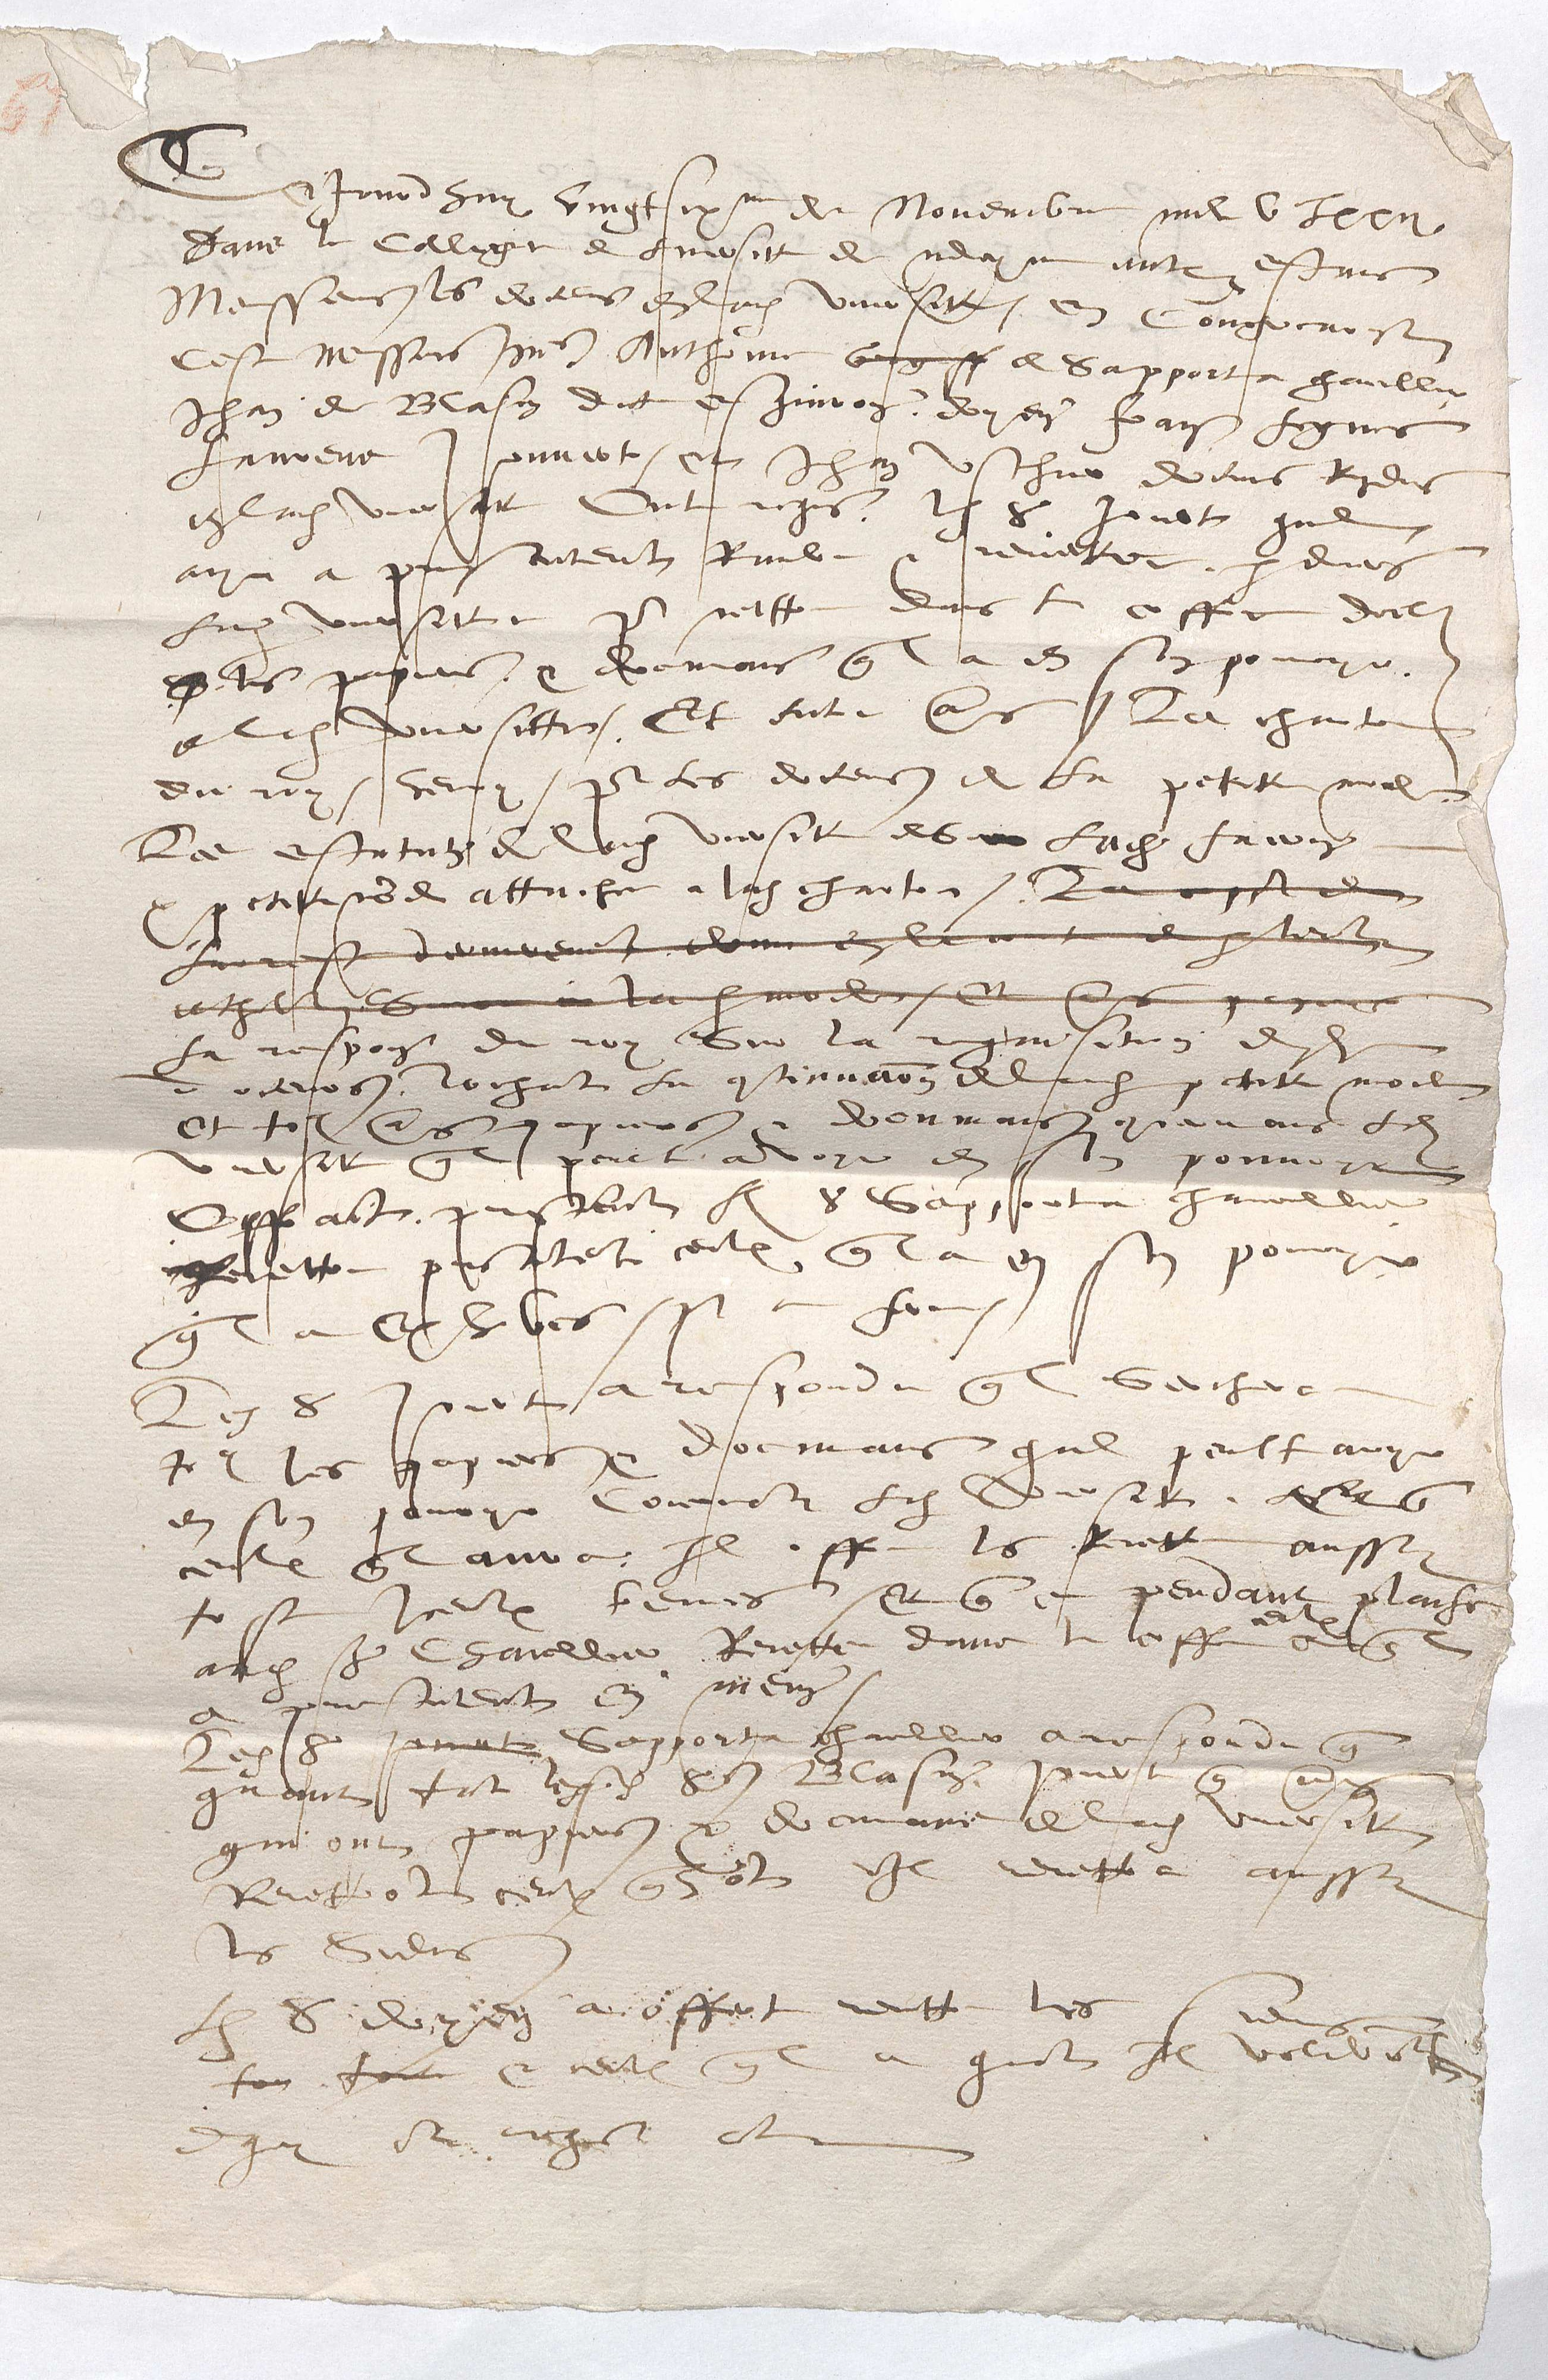
\includegraphics[
	width=\textwidth,
	height=0.65\textheight,
	keepaspectratio
	]{images/C17_01.jpg}
	
	\vspace{0.6em}
	
	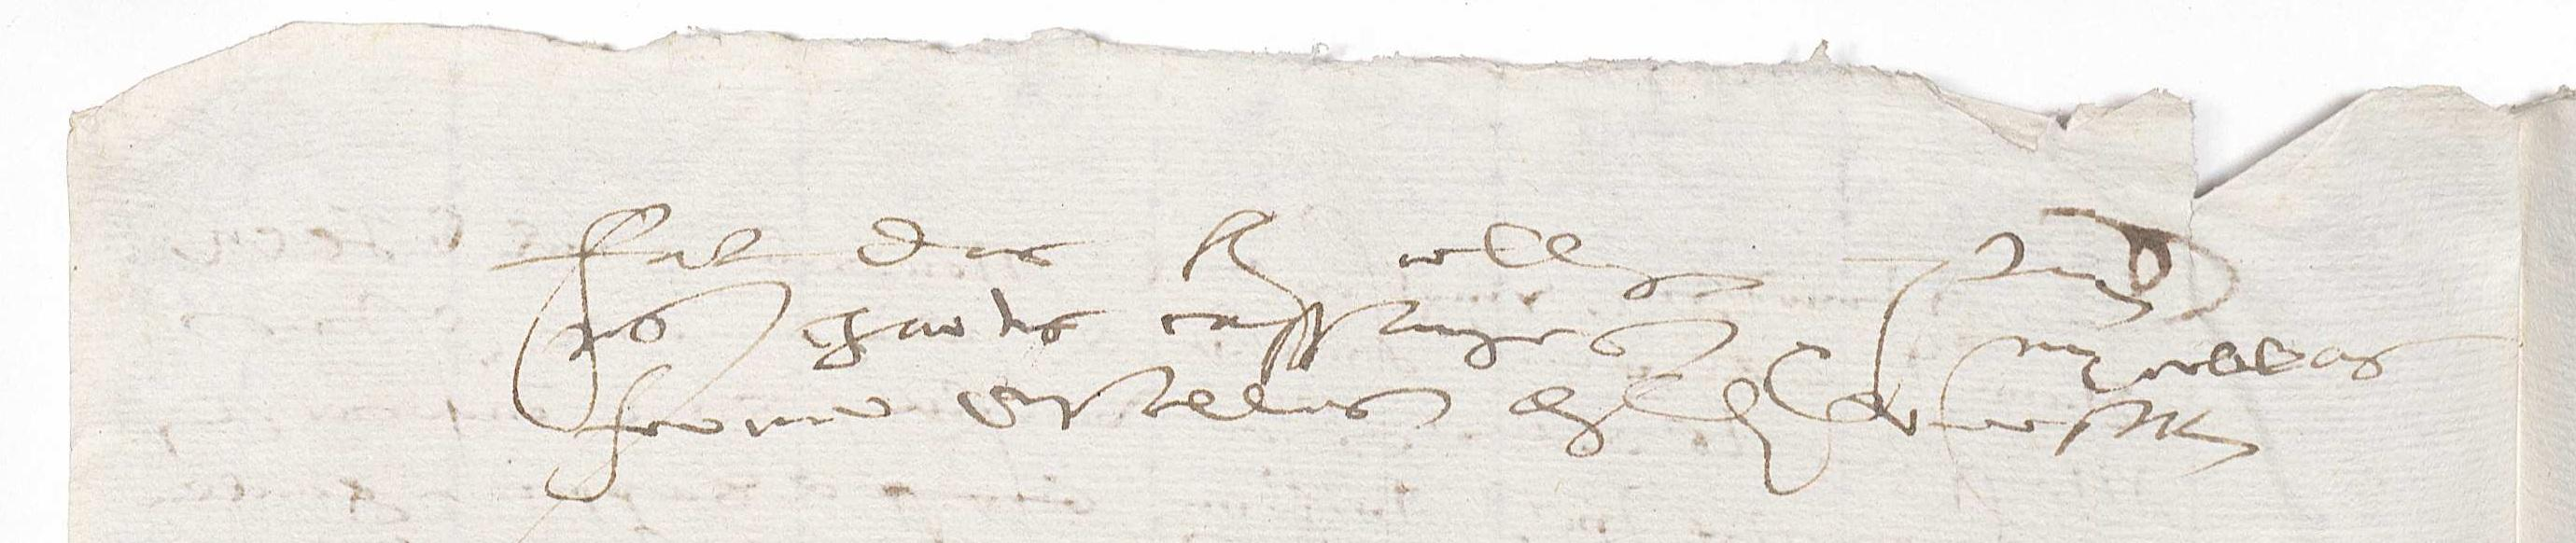
\includegraphics[
	width=\textwidth,
	height=0.12\textheight,
	keepaspectratio
	]{images/C17_02.jpg}
	
	\caption[Délibération demandant à Laurent Joubert de remettre des papiers de l'Université]
	{\enquote{Délibération en vertu de laquelle Laurent Joubert est invité à remettre certains papiers de l'Université qui sont entre ses mains}, 26 novembre 1572, recto et détail du verso recadré sur le passage final, Montpellier, Archives historiques de la Faculté de médecine, C~17. Numérisation : Clara Martin.}
	\label{fig:c17}
\end{figure}

\begin{figure}[p]
	\centering
	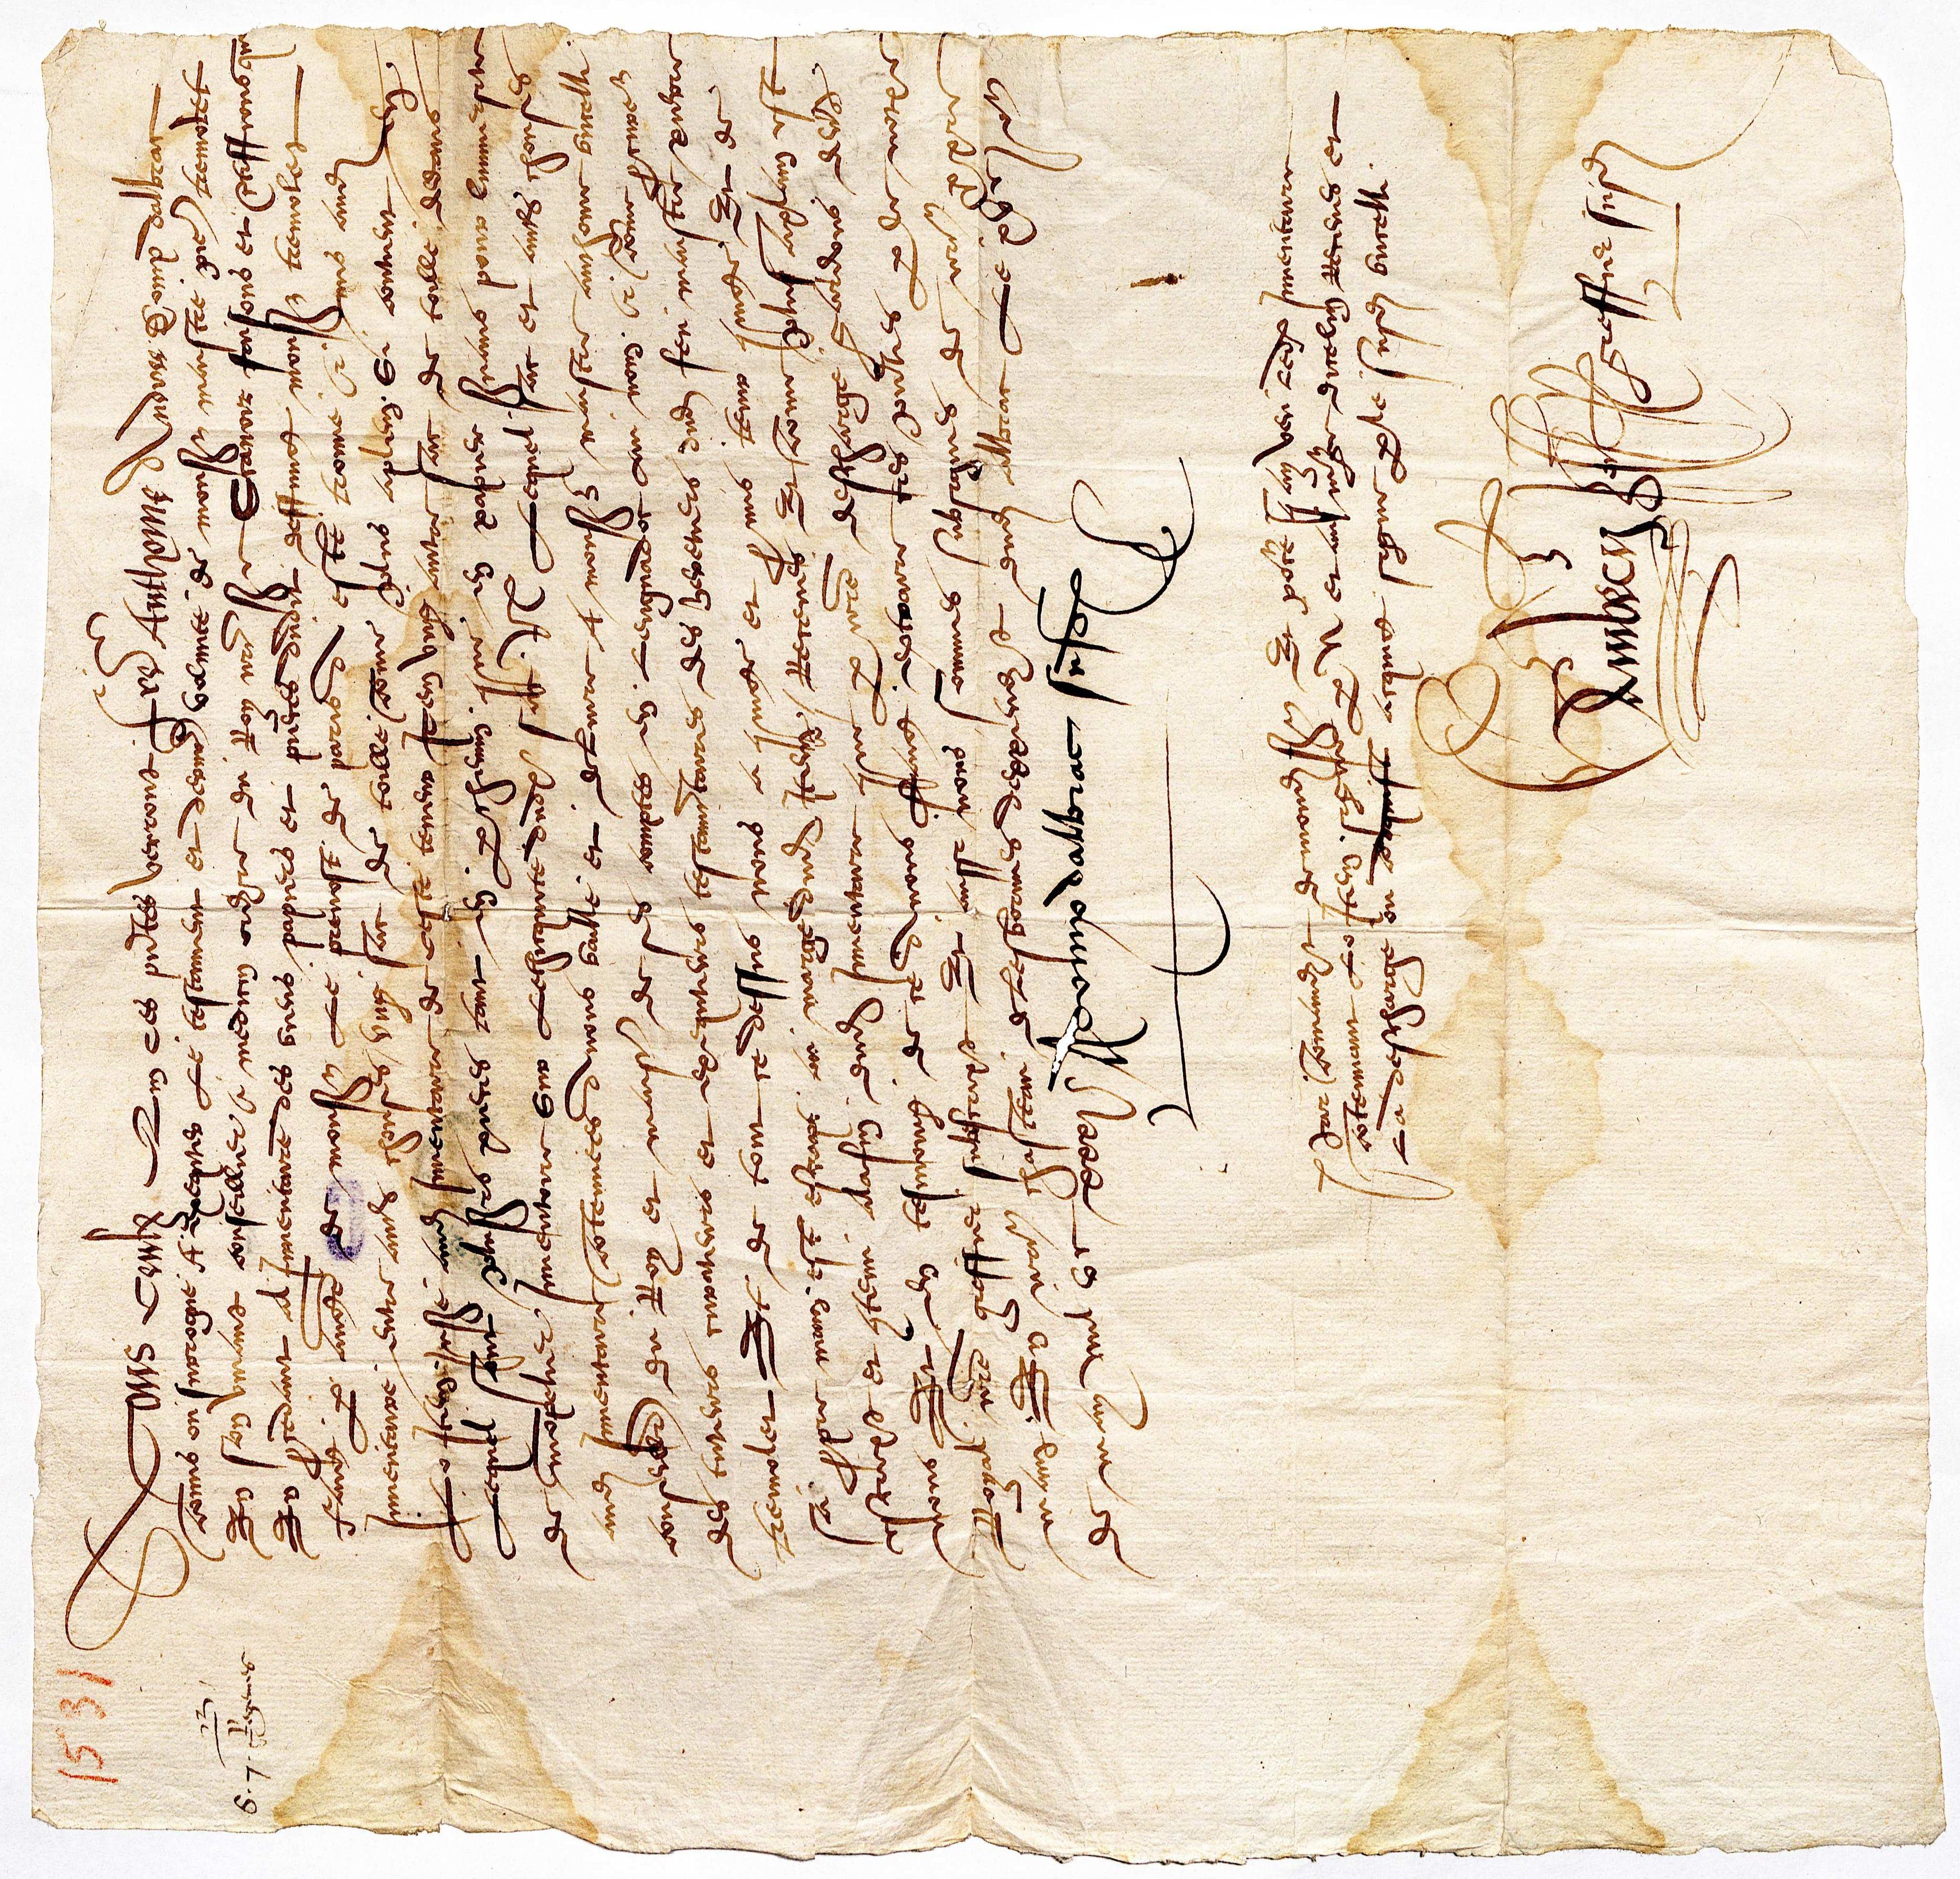
\includegraphics[
	angle=270,
	origin=c,
	width=\textwidth,
	height=0.82\textheight,
	keepaspectratio
	]{images/C4_01.jpg}
	\caption[Restitution à l'Université des papiers de Pierre Trémolet]
	{\enquote{Restitution de papiers appartenant à l'Université et trouvés dans la succession de feu Pierre Trémolet, docteur décédé à Paris}, 15 mai 1531, recto, Montpellier, Archives historiques de la Faculté de médecine, C~4 (ancienne cote : sac~7~B). Numérisation : Clara Martin.}
	\label{fig:c4-recto}
\end{figure}

\begin{figure}[p]
	\centering
	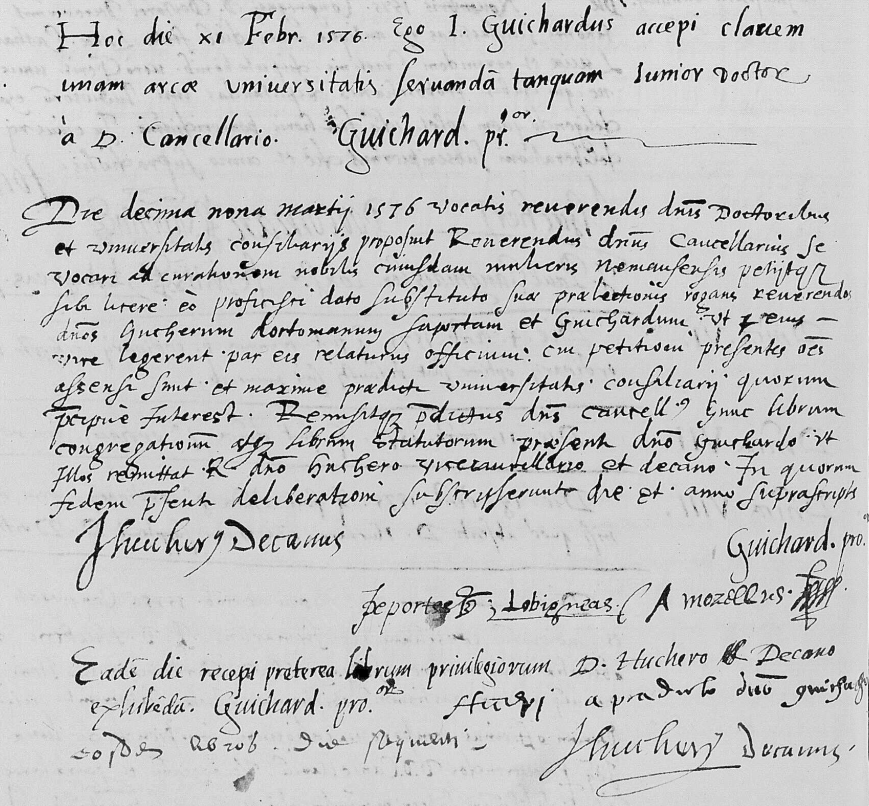
\includegraphics[
	width=\textwidth,
	height=0.78\textheight,
	keepaspectratio
	]{images/S8_f90v.png}
	\caption[Remise d'une clé du coffre et du livre des privilèges au procureur Guichard]
	{\enquote{Reconnaissance par le procureur Guichard de la remise d'une clé du coffre et du livre des privilèges}, 11 février 1576, détail du fol.~90~v\textsuperscript{o} recadré sur le passage concerné, dans le \emph{Liber congregationum Universitatis Monspeliensis}, registre des délibérations, actes et examens, 1557--1598, Montpellier, Archives historiques de la Faculté de médecine, S~8. Numérisation : Clara Martin.}
	\label{fig:s8-f90v}
\end{figure}

\begin{figure}[p]
	\centering
	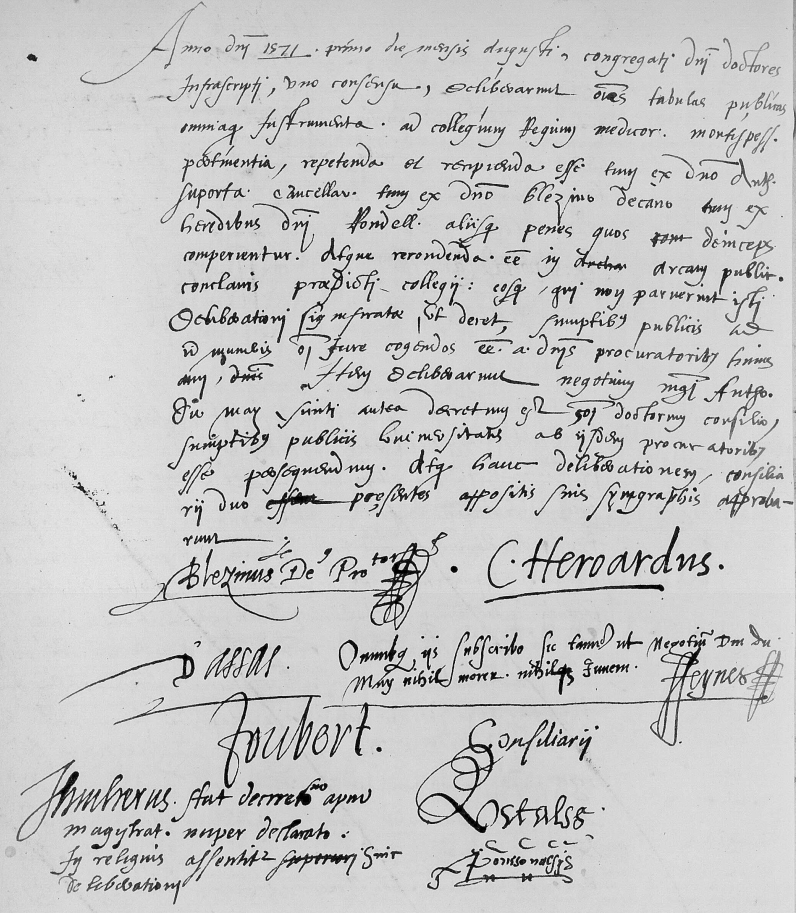
\includegraphics[
	width=\textwidth,
	height=0.78\textheight,
	keepaspectratio
	]{images/S8_f51.png}
	\caption[Réunion des archives dans le coffre public de la salle du Collège]
	{\enquote{Délibération prescrivant la récupération des actes et registres appartenant au Collège des médecins et leur dépôt dans le coffre public de la salle du Collège}, 1\textsuperscript{er} août 1571, fol.~51~v\textsuperscript{o}, dans le \emph{Liber congregationum Universitatis Monspeliensis}, registre des délibérations, actes et examens, 1557--1598, Montpellier, Archives historiques de la Faculté de médecine, S~8. Numérisation : Clara Martin.}
	\label{fig:s8-f51v}
\end{figure}

\begin{figure}[p]
	\centering
	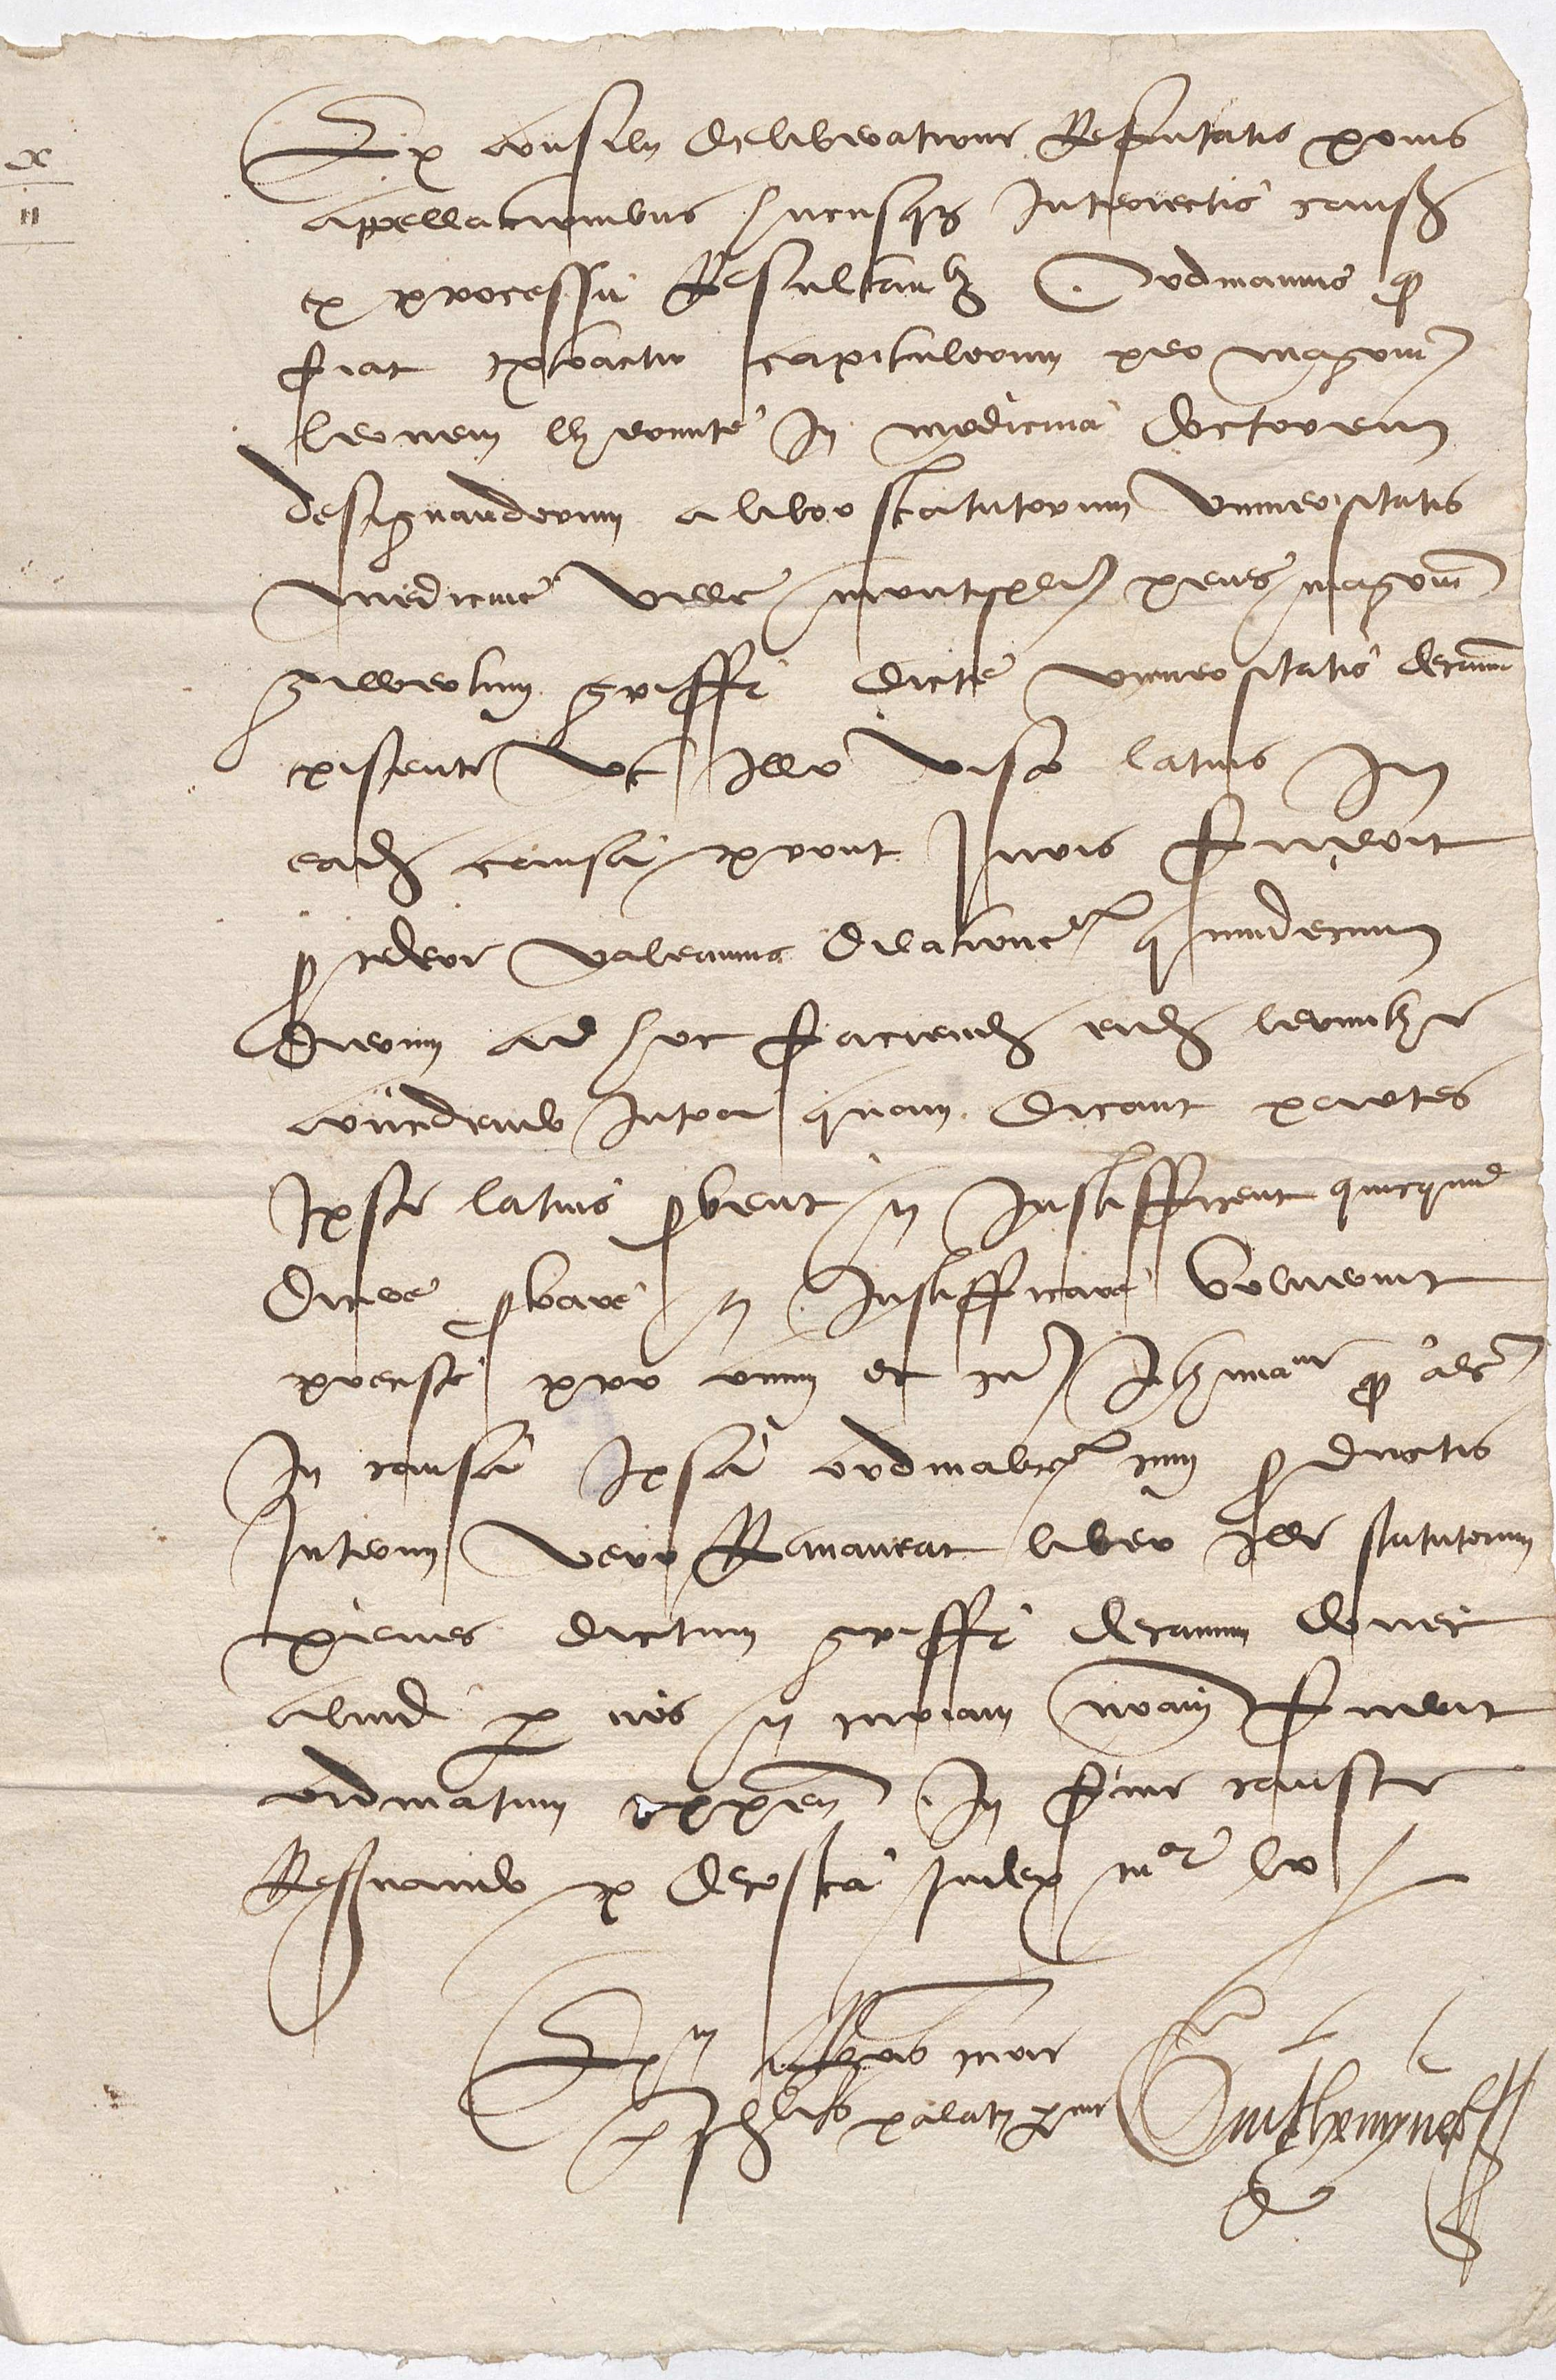
\includegraphics[
	width=\textwidth,
	height=0.78\textheight,
	keepaspectratio
	]{images/C9.jpg}
	\caption[Autorisation donnée à Lermite de faire des extraits des statuts]
	{\enquote{Procès-verbal d'une délibération en vertu de laquelle Lermite, docteur, est autorisé à faire certains extraits des statuts, dans les registres qui sont entre les mains du doyen Gilbert Griffi}, s. d., Montpellier, Archives historiques de la Faculté de médecine, C~9 (ancienne cote : sac~11~X). Numérisation : Clara Martin.}
	\label{fig:c9}
\end{figure}

\begin{figure}[p]
	\centering
	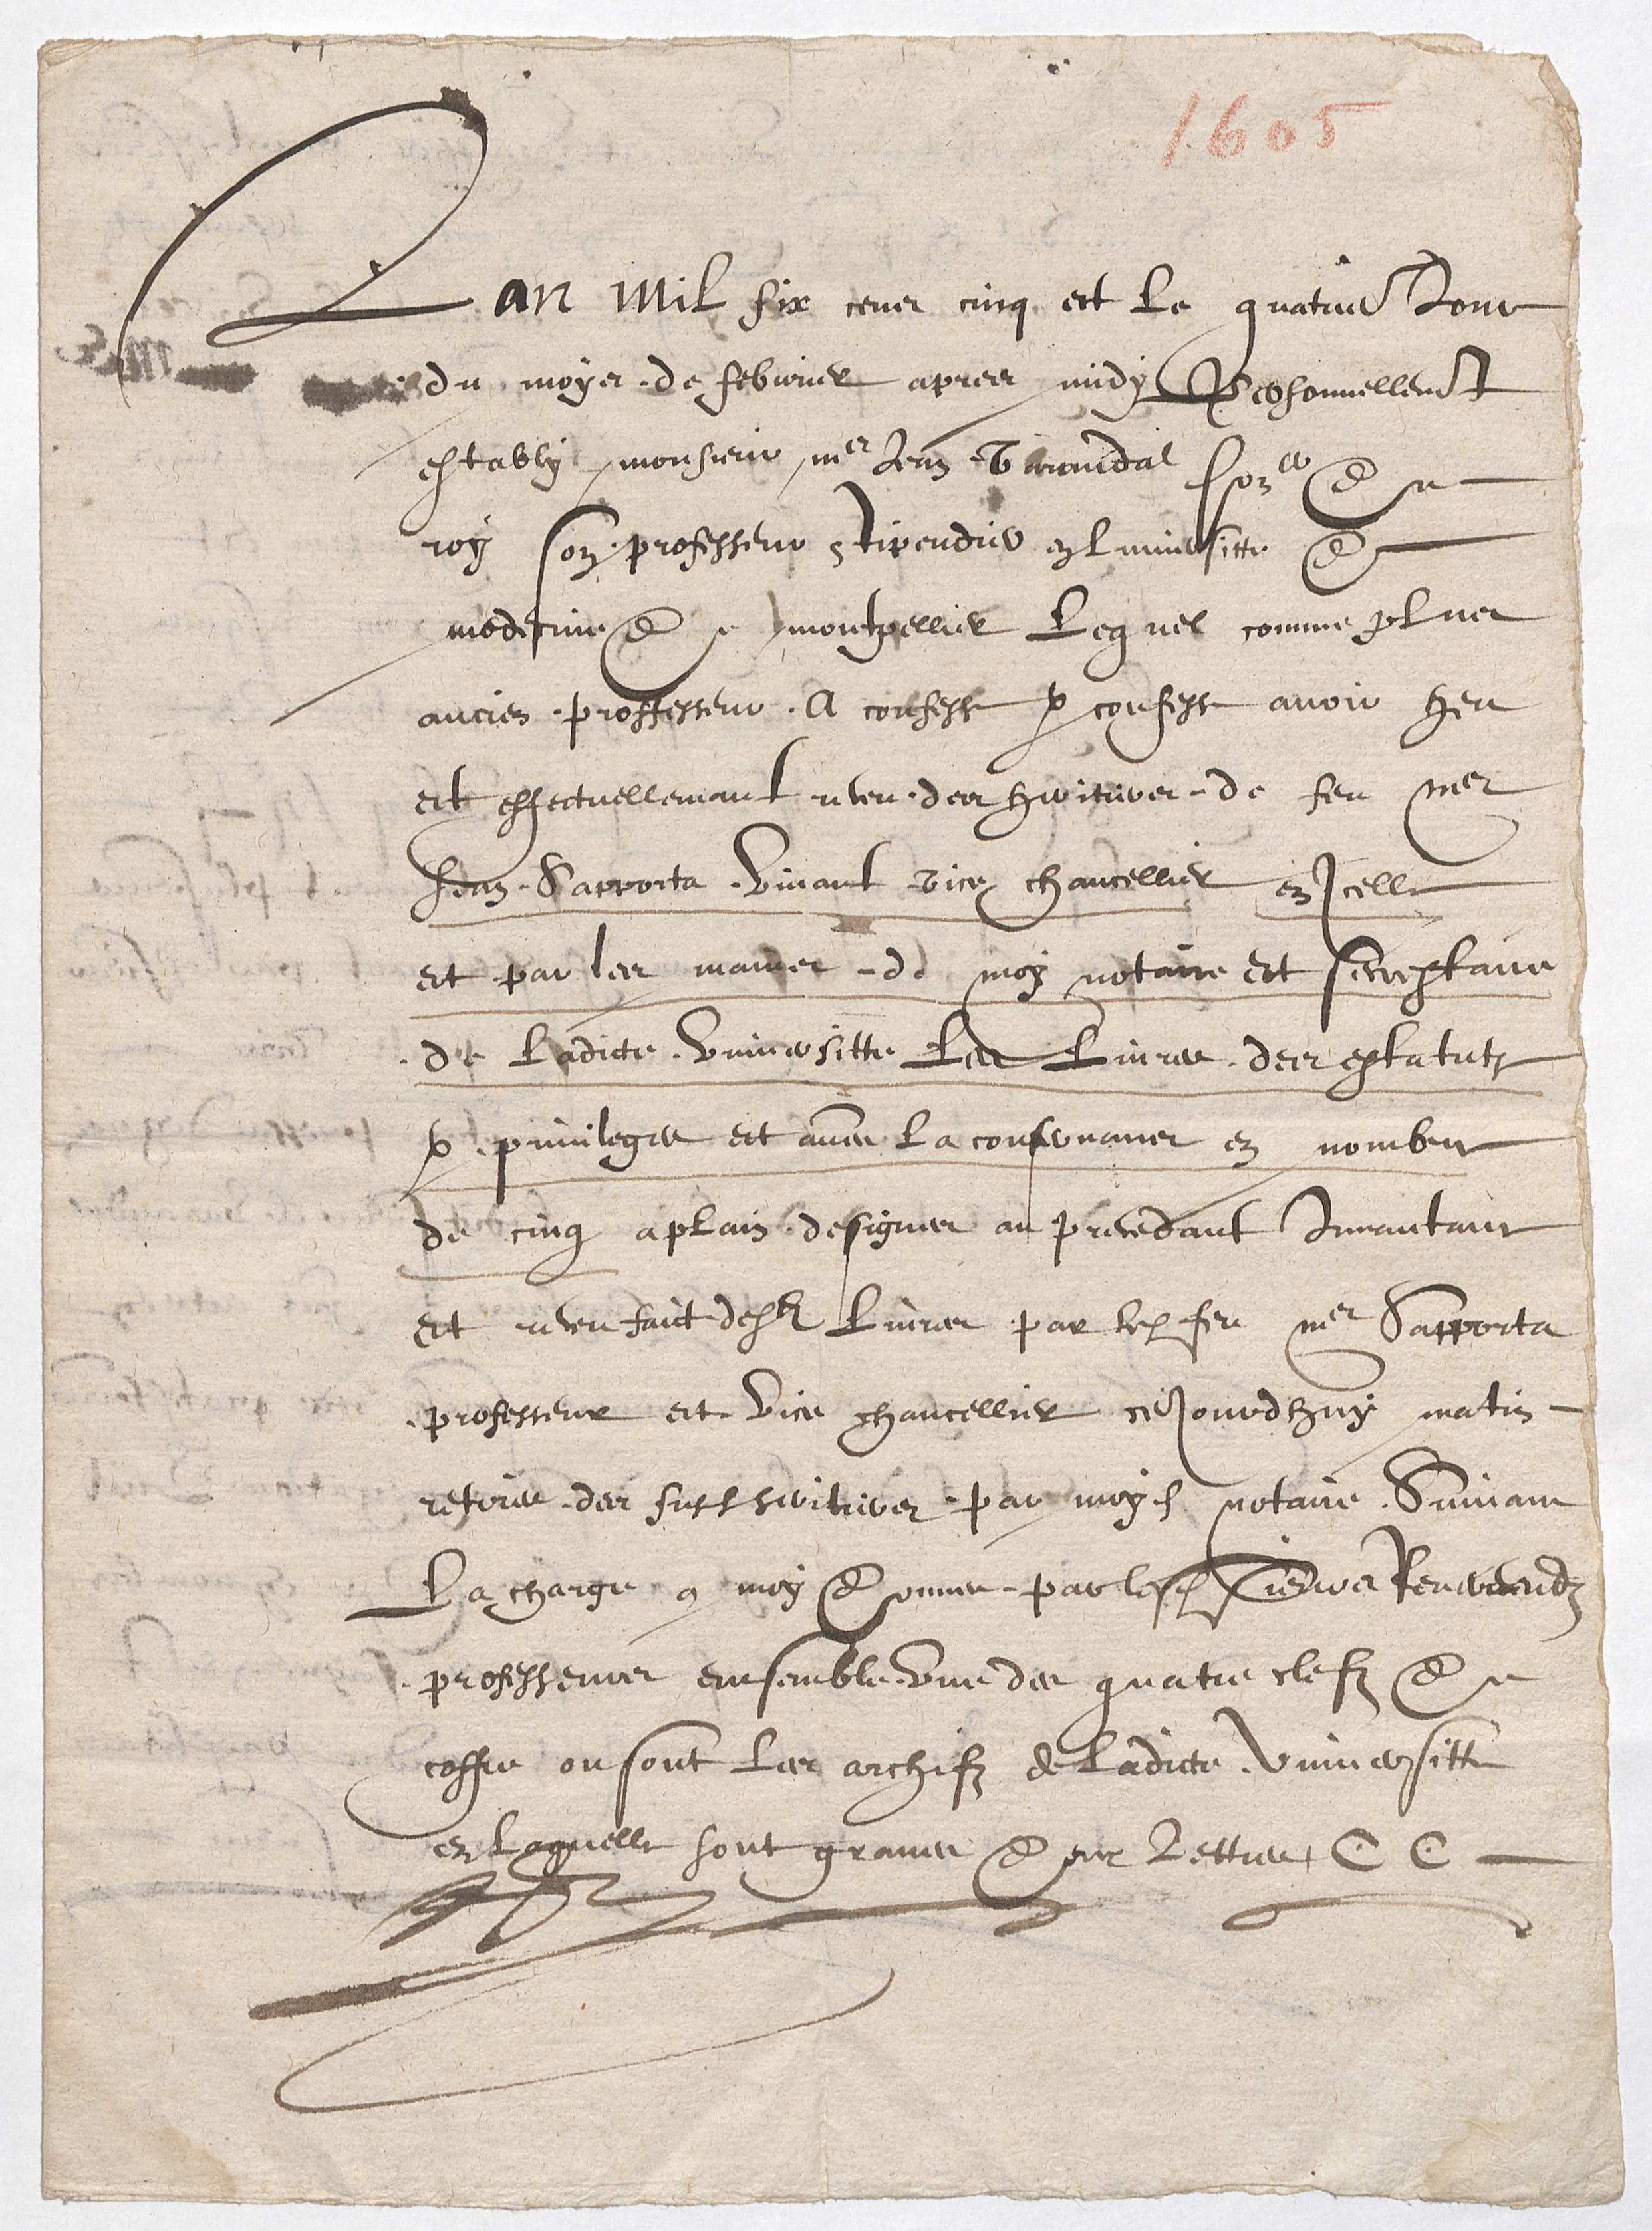
\includegraphics[
	width=\textwidth,
	height=0.78\textheight,
	keepaspectratio
	]{images/C35_01.jpg}
	\caption[Remise des archives à Jean Varanda en qualité de plus ancien docteur]
	{\enquote{Remise des archives à Jean Varanda en qualité de plus ancien docteur}, 4 février 1605, première vue, Montpellier, Archives historiques de la Faculté de médecine, C~35. Numérisation : Clara Martin.}
	\label{fig:c35-01}
\end{figure}

\clearpage

\begin{landscape}
	\begin{figure}[p]
		\centering
		
		\rotatebox{180}{%
			\begin{minipage}{\linewidth}
				\centering
				
				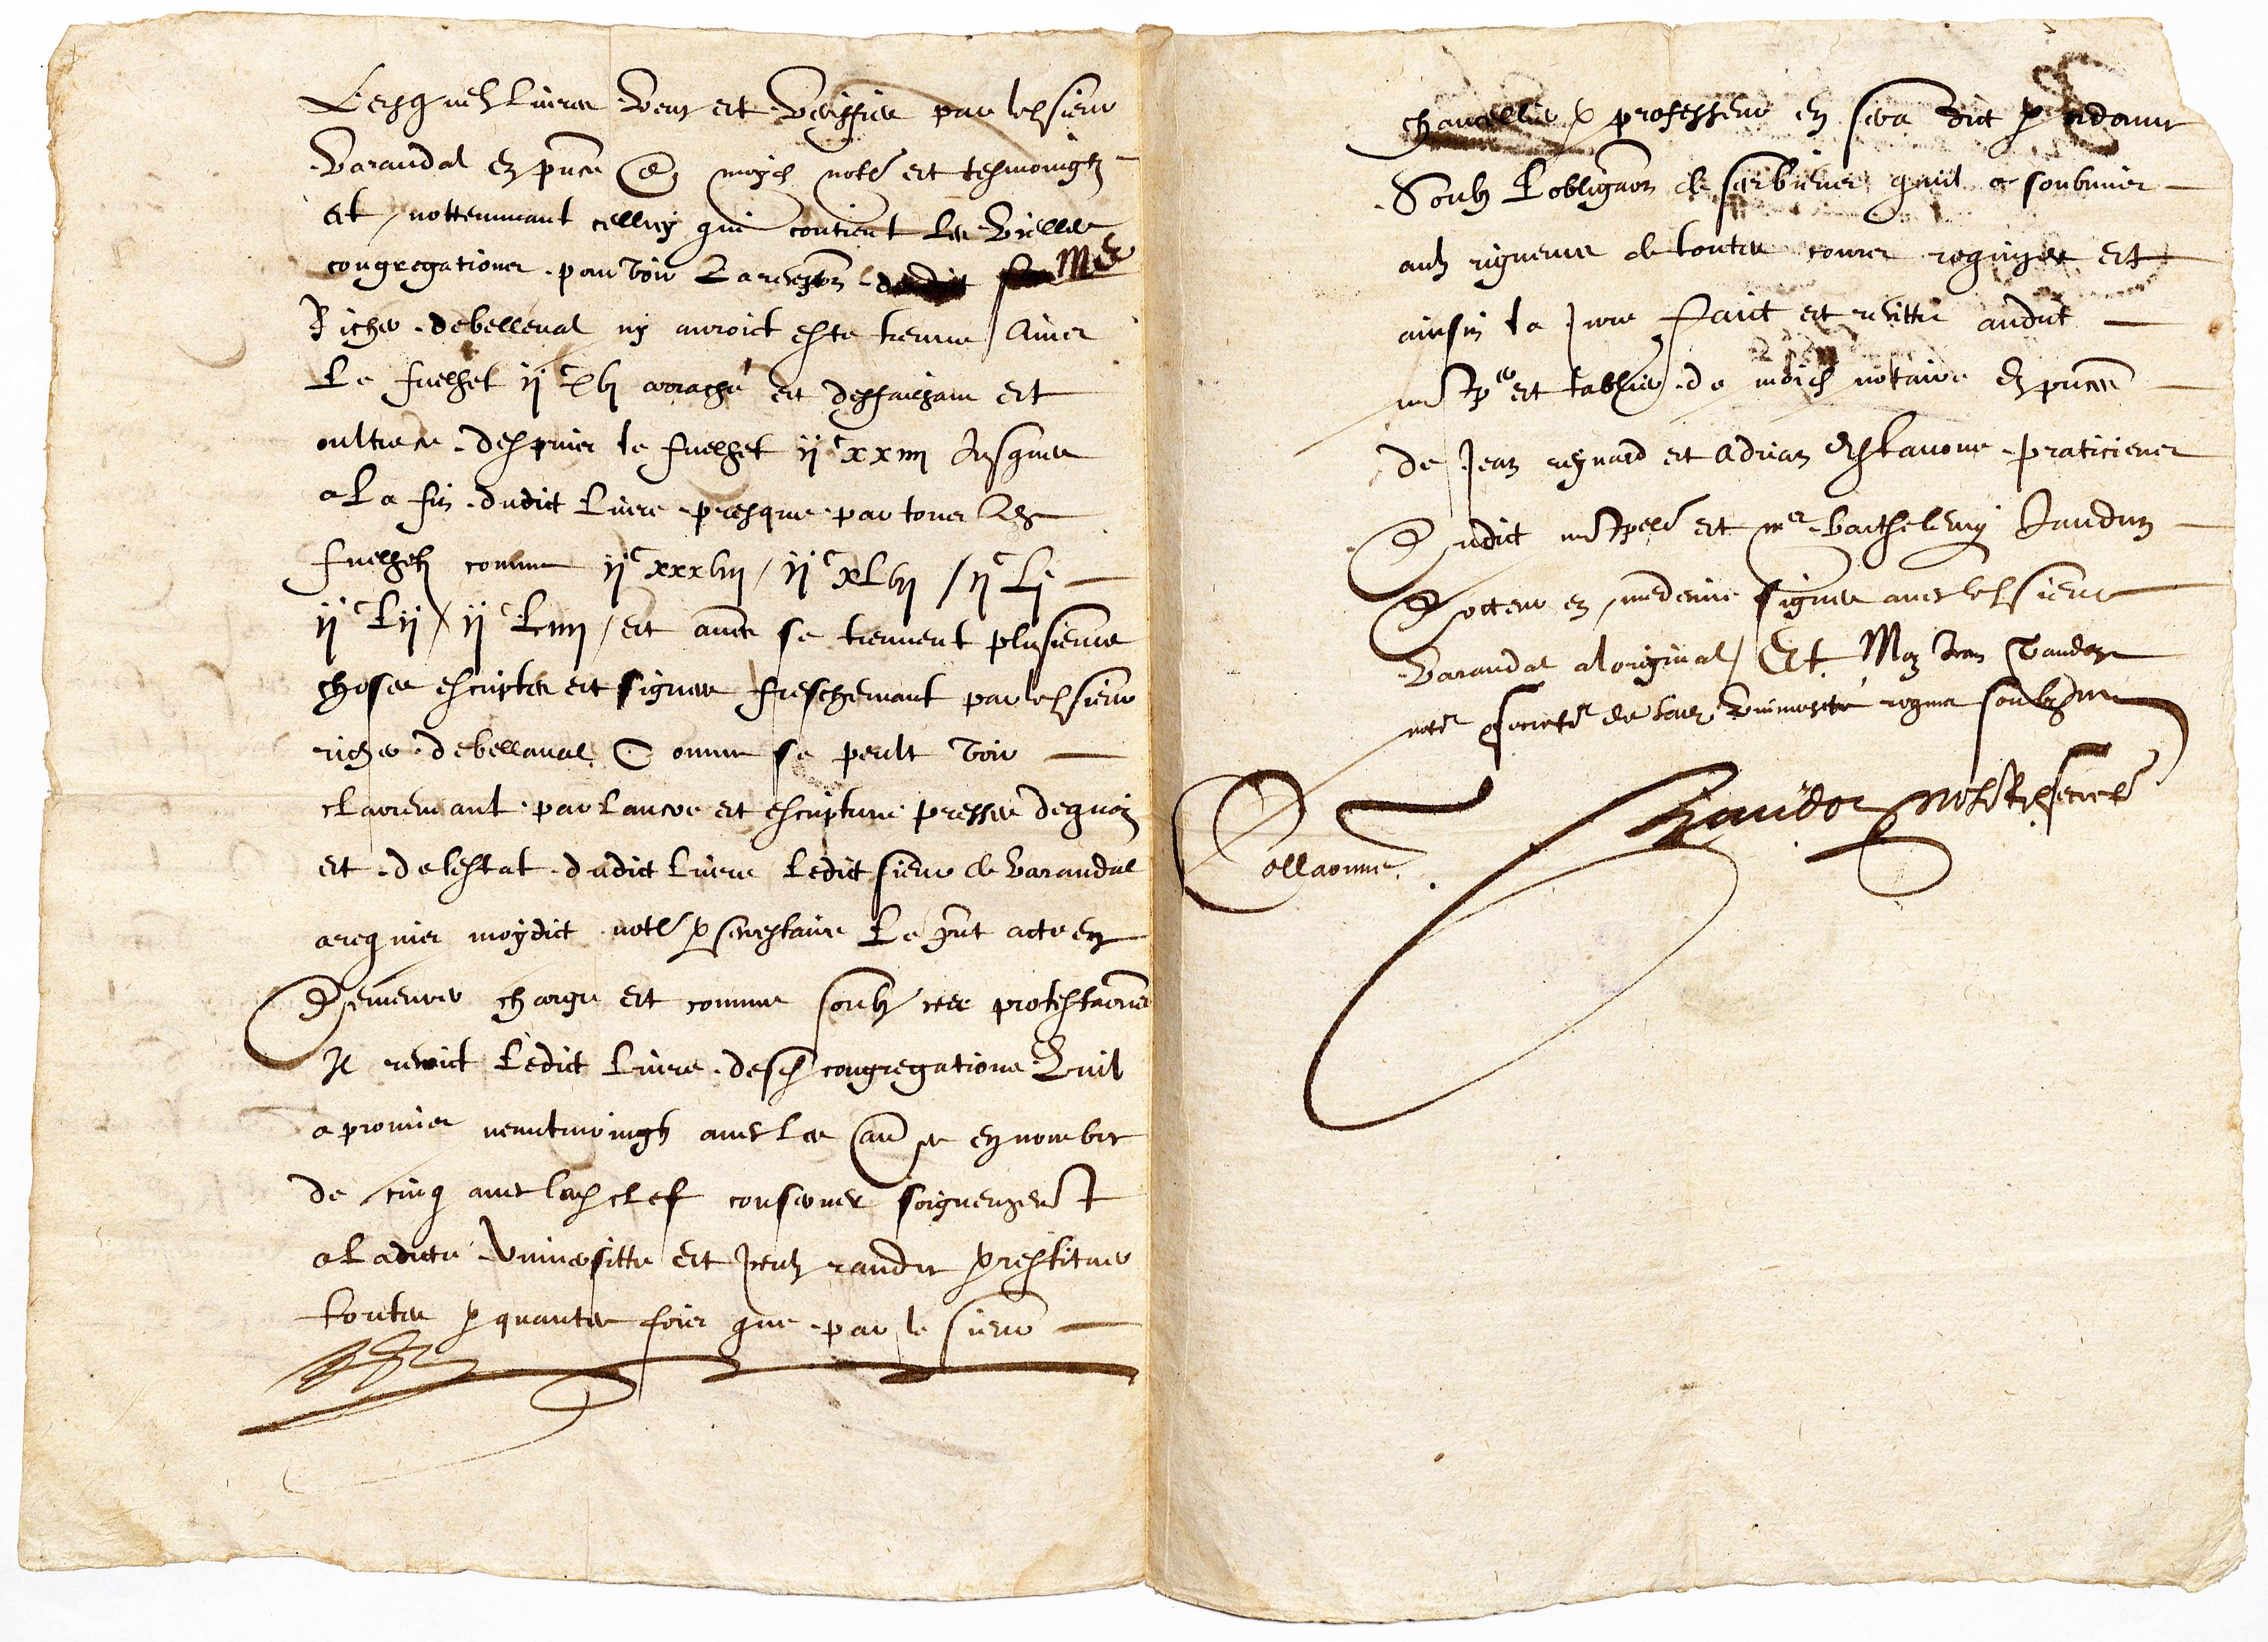
\includegraphics[
				width=0.92\linewidth,
				keepaspectratio
				]{images/C35_02.jpg}
				
				\captionof{figure}
				[Remise des archives à Jean Varanda en qualité de plus ancien docteur]
				{\enquote{Remise des archives à Jean Varanda en qualité de plus ancien docteur}, 4 février 1605, seconde vue, Montpellier, Archives historiques de la Faculté de médecine, C~35. Numérisation : Clara Martin.}
				
				\label{fig:c35-02}
				
			\end{minipage}%
		}
		
	\end{figure}
\end{landscape}

\begin{figure}[p]
	\centering
	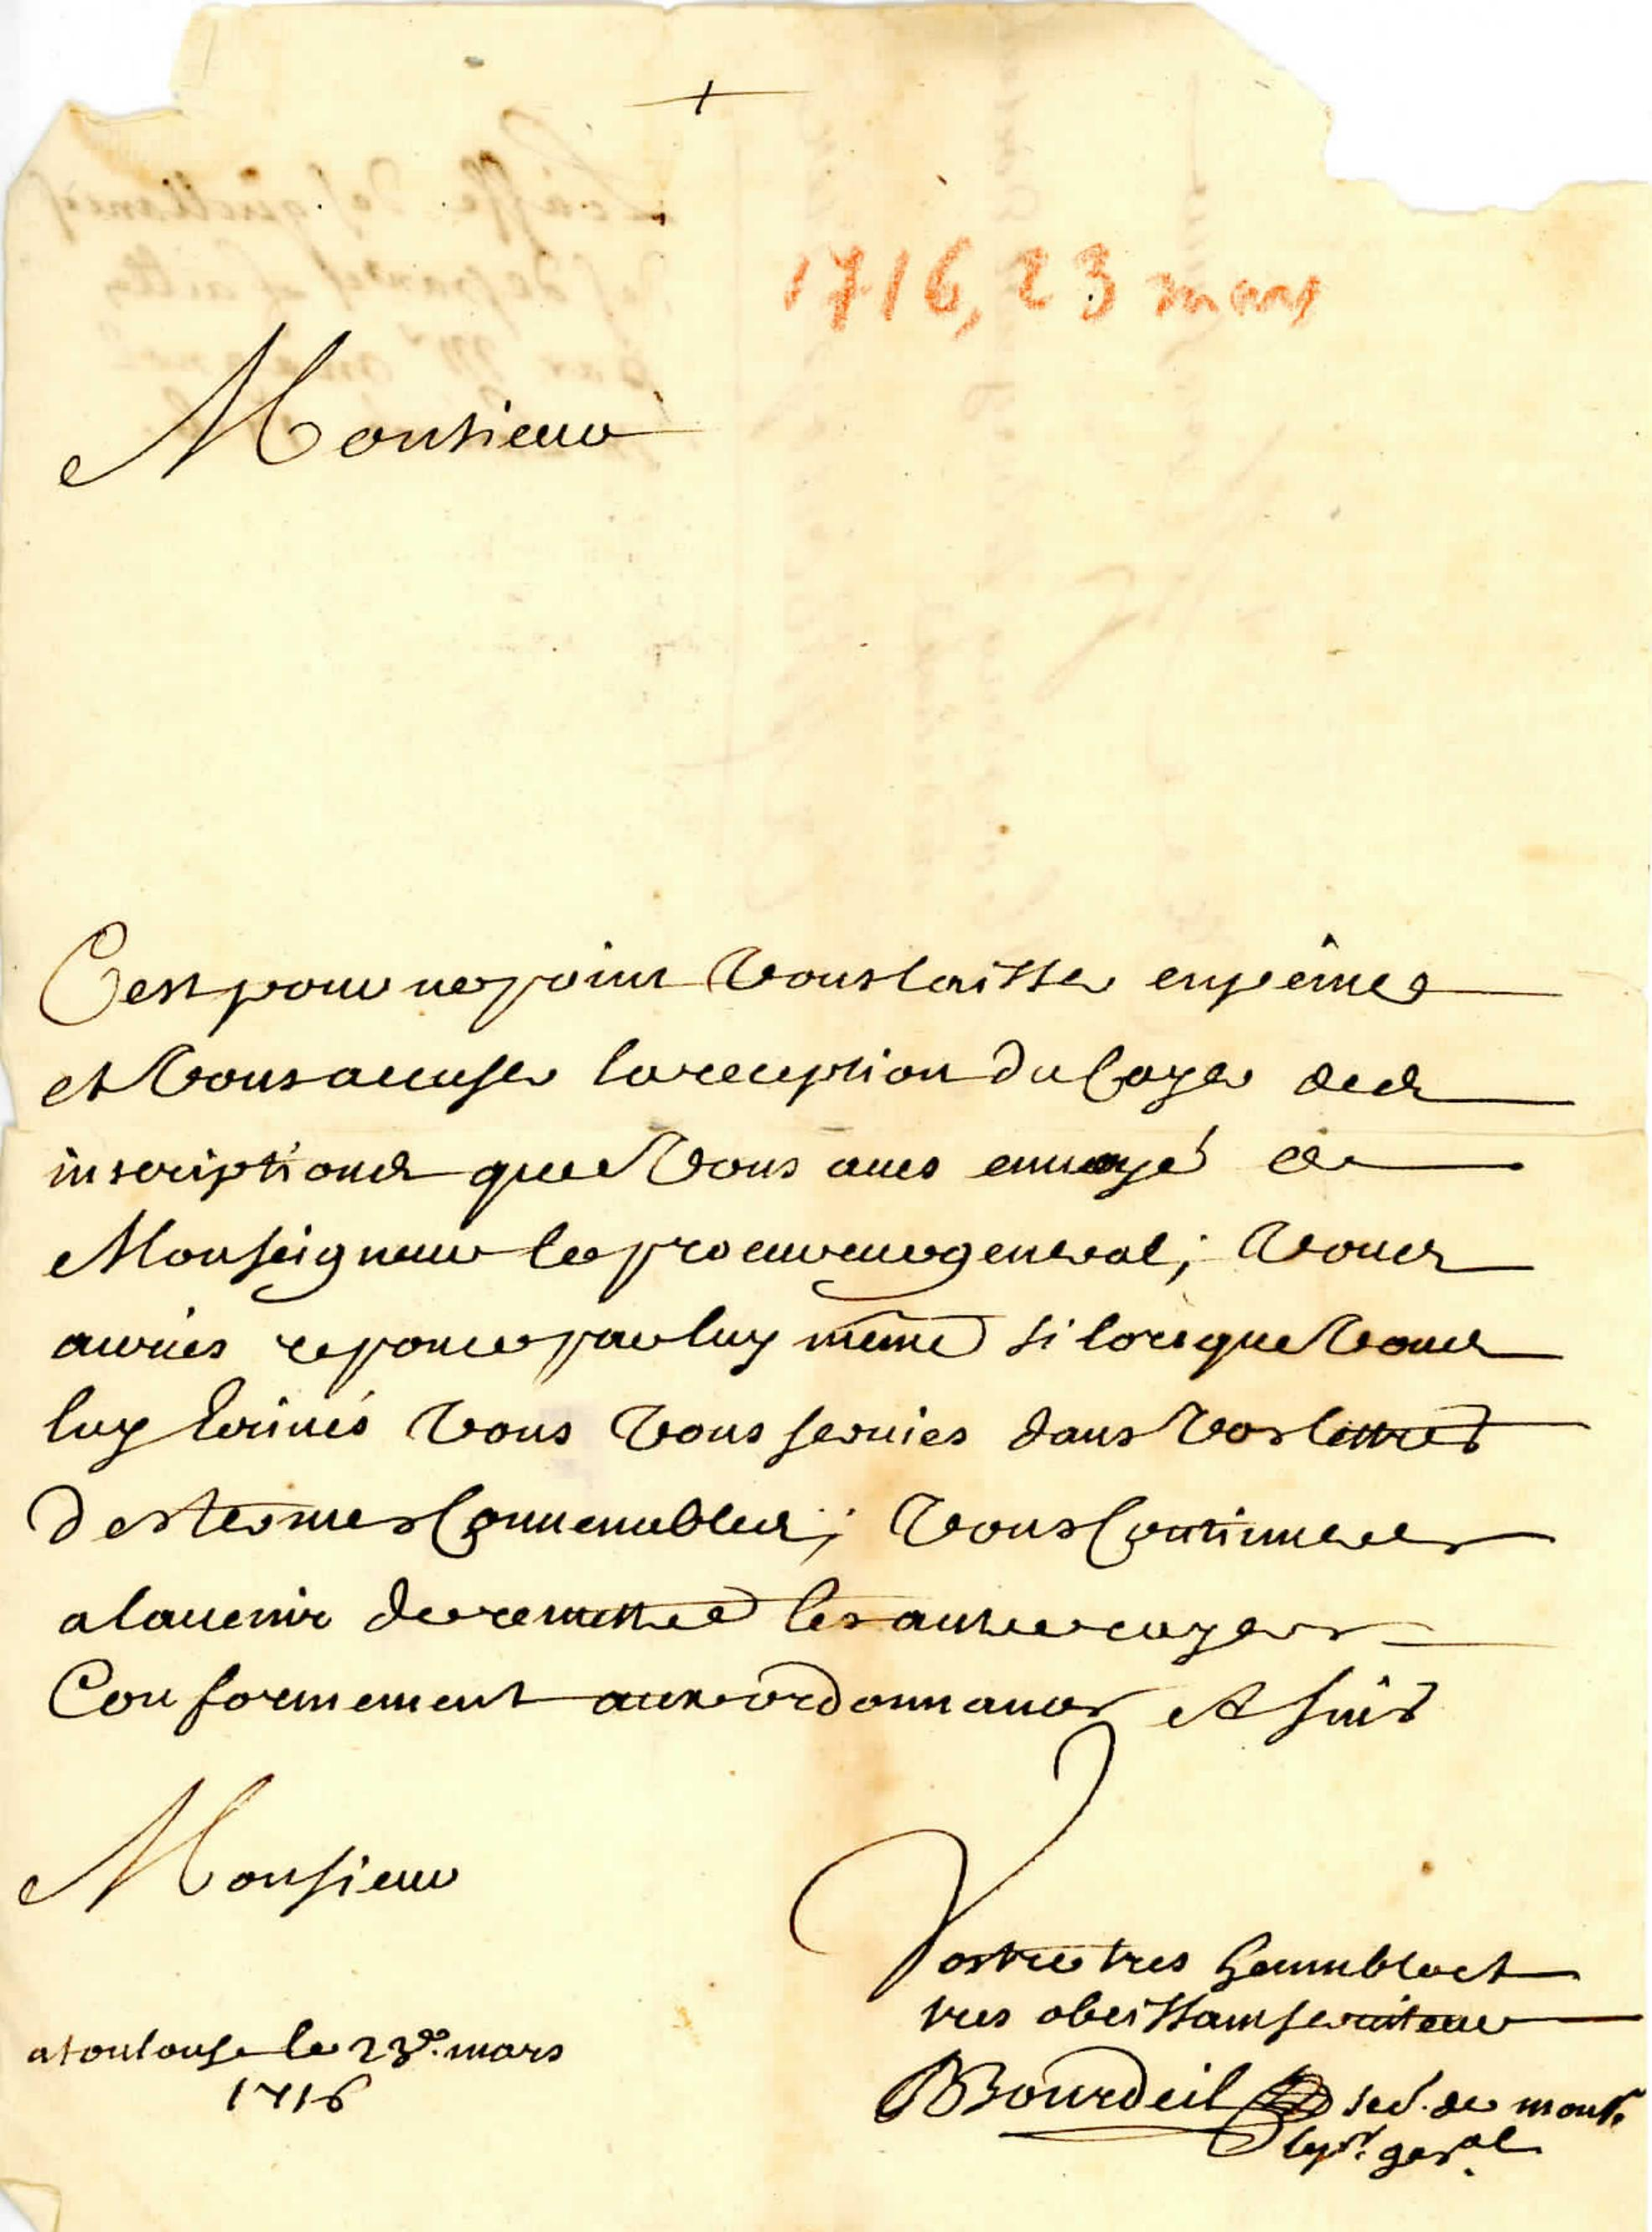
\includegraphics[
	width=\textwidth,
	height=0.78\textheight,
	keepaspectratio
	]{images/F24_01.jpg}
	\caption[Lettre accusant réception d'un registre d'inscription, recto]
	{\enquote{Lettre du sieur de Bourdeil, secrétaire de M. le Procureur général, pour accuser réception d'un registre d'inscription}, recto, Toulouse, 23 mars 1716, Montpellier, Archives historiques de la Faculté de médecine, F~24. Numérisation : Clara Martin.}
	\label{fig:f24-01}
\end{figure}

\begin{figure}[p]
	\centering
	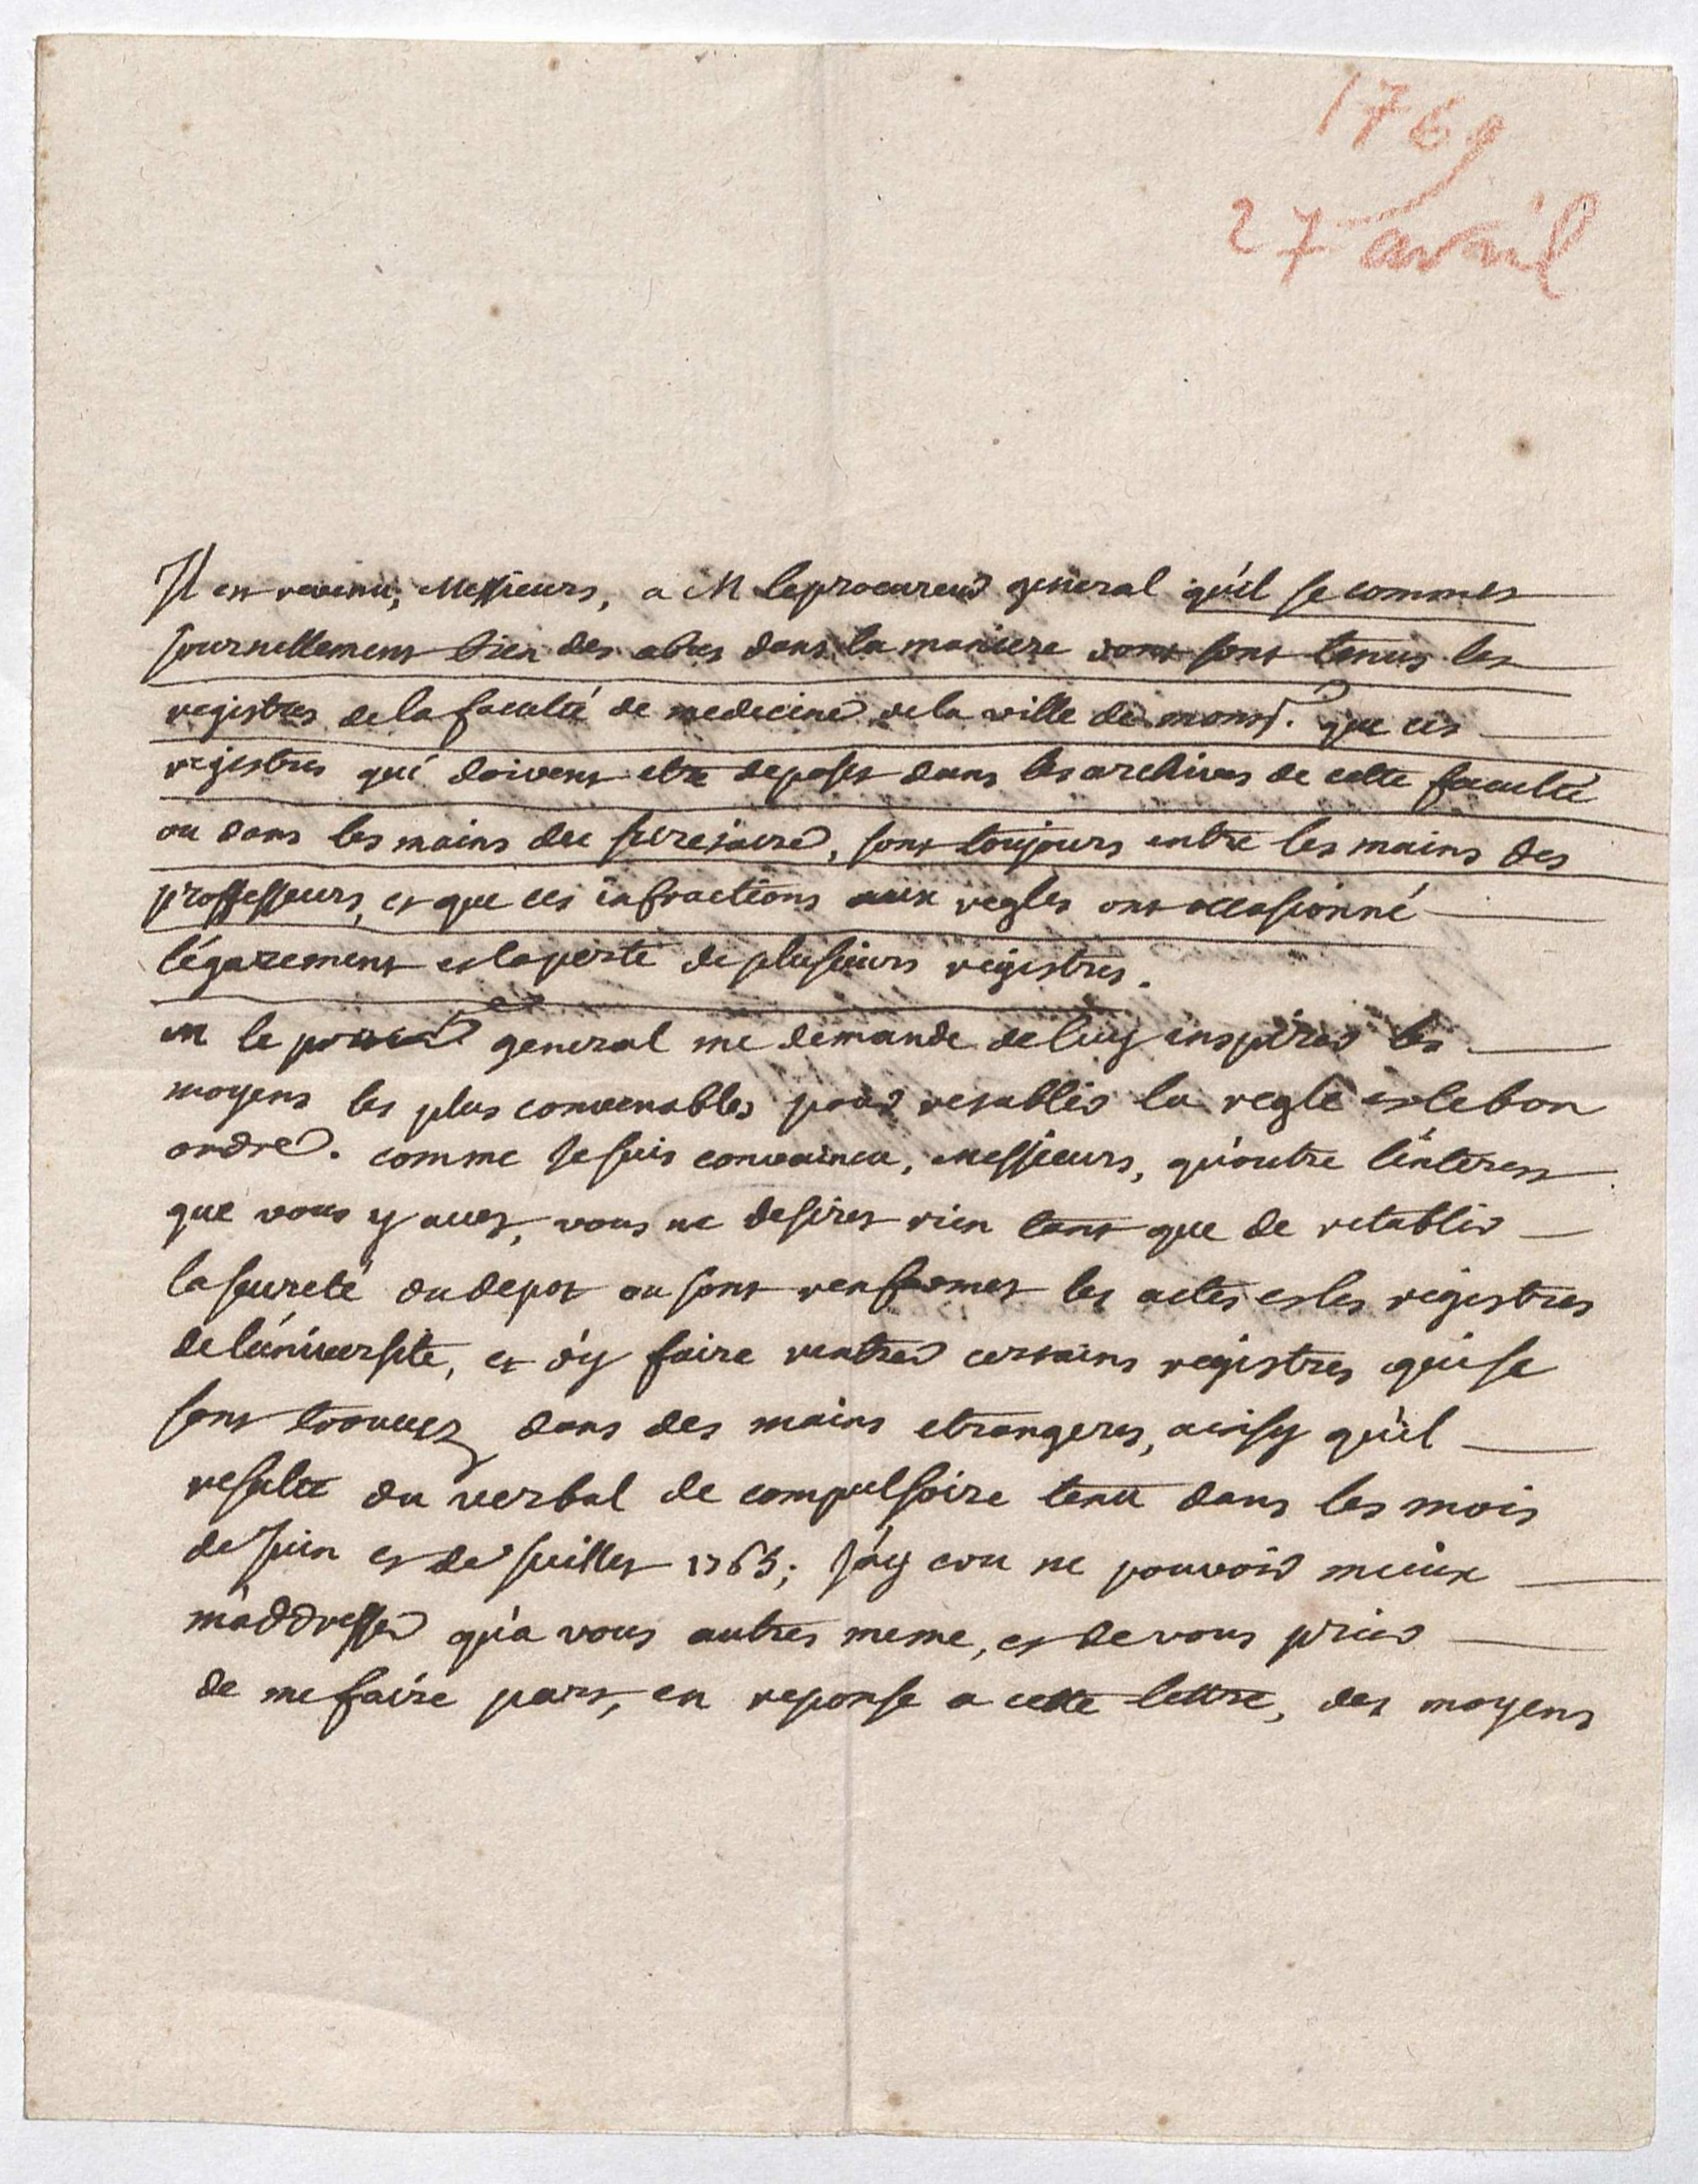
\includegraphics[
	width=\textwidth,
	height=0.78\textheight,
	keepaspectratio
	]{images/F54_19.jpg}
	\caption[Lettre relative à la mauvaise tenue des archives, première vue]
	{\enquote{Lettre écrite au nom du procureur général au sujet de la mauvaise tenue des archives de la Faculté et sur les mesures qu'il serait indispensable de prendre pour éviter la perte des documents}, première vue, 27 avril 1769, sans lieu, Montpellier, Archives historiques de la Faculté de médecine, F~54. Numérisation : Clara Martin.}
	\label{fig:f54-19}
\end{figure}

\begin{figure}[p]
	\centering
	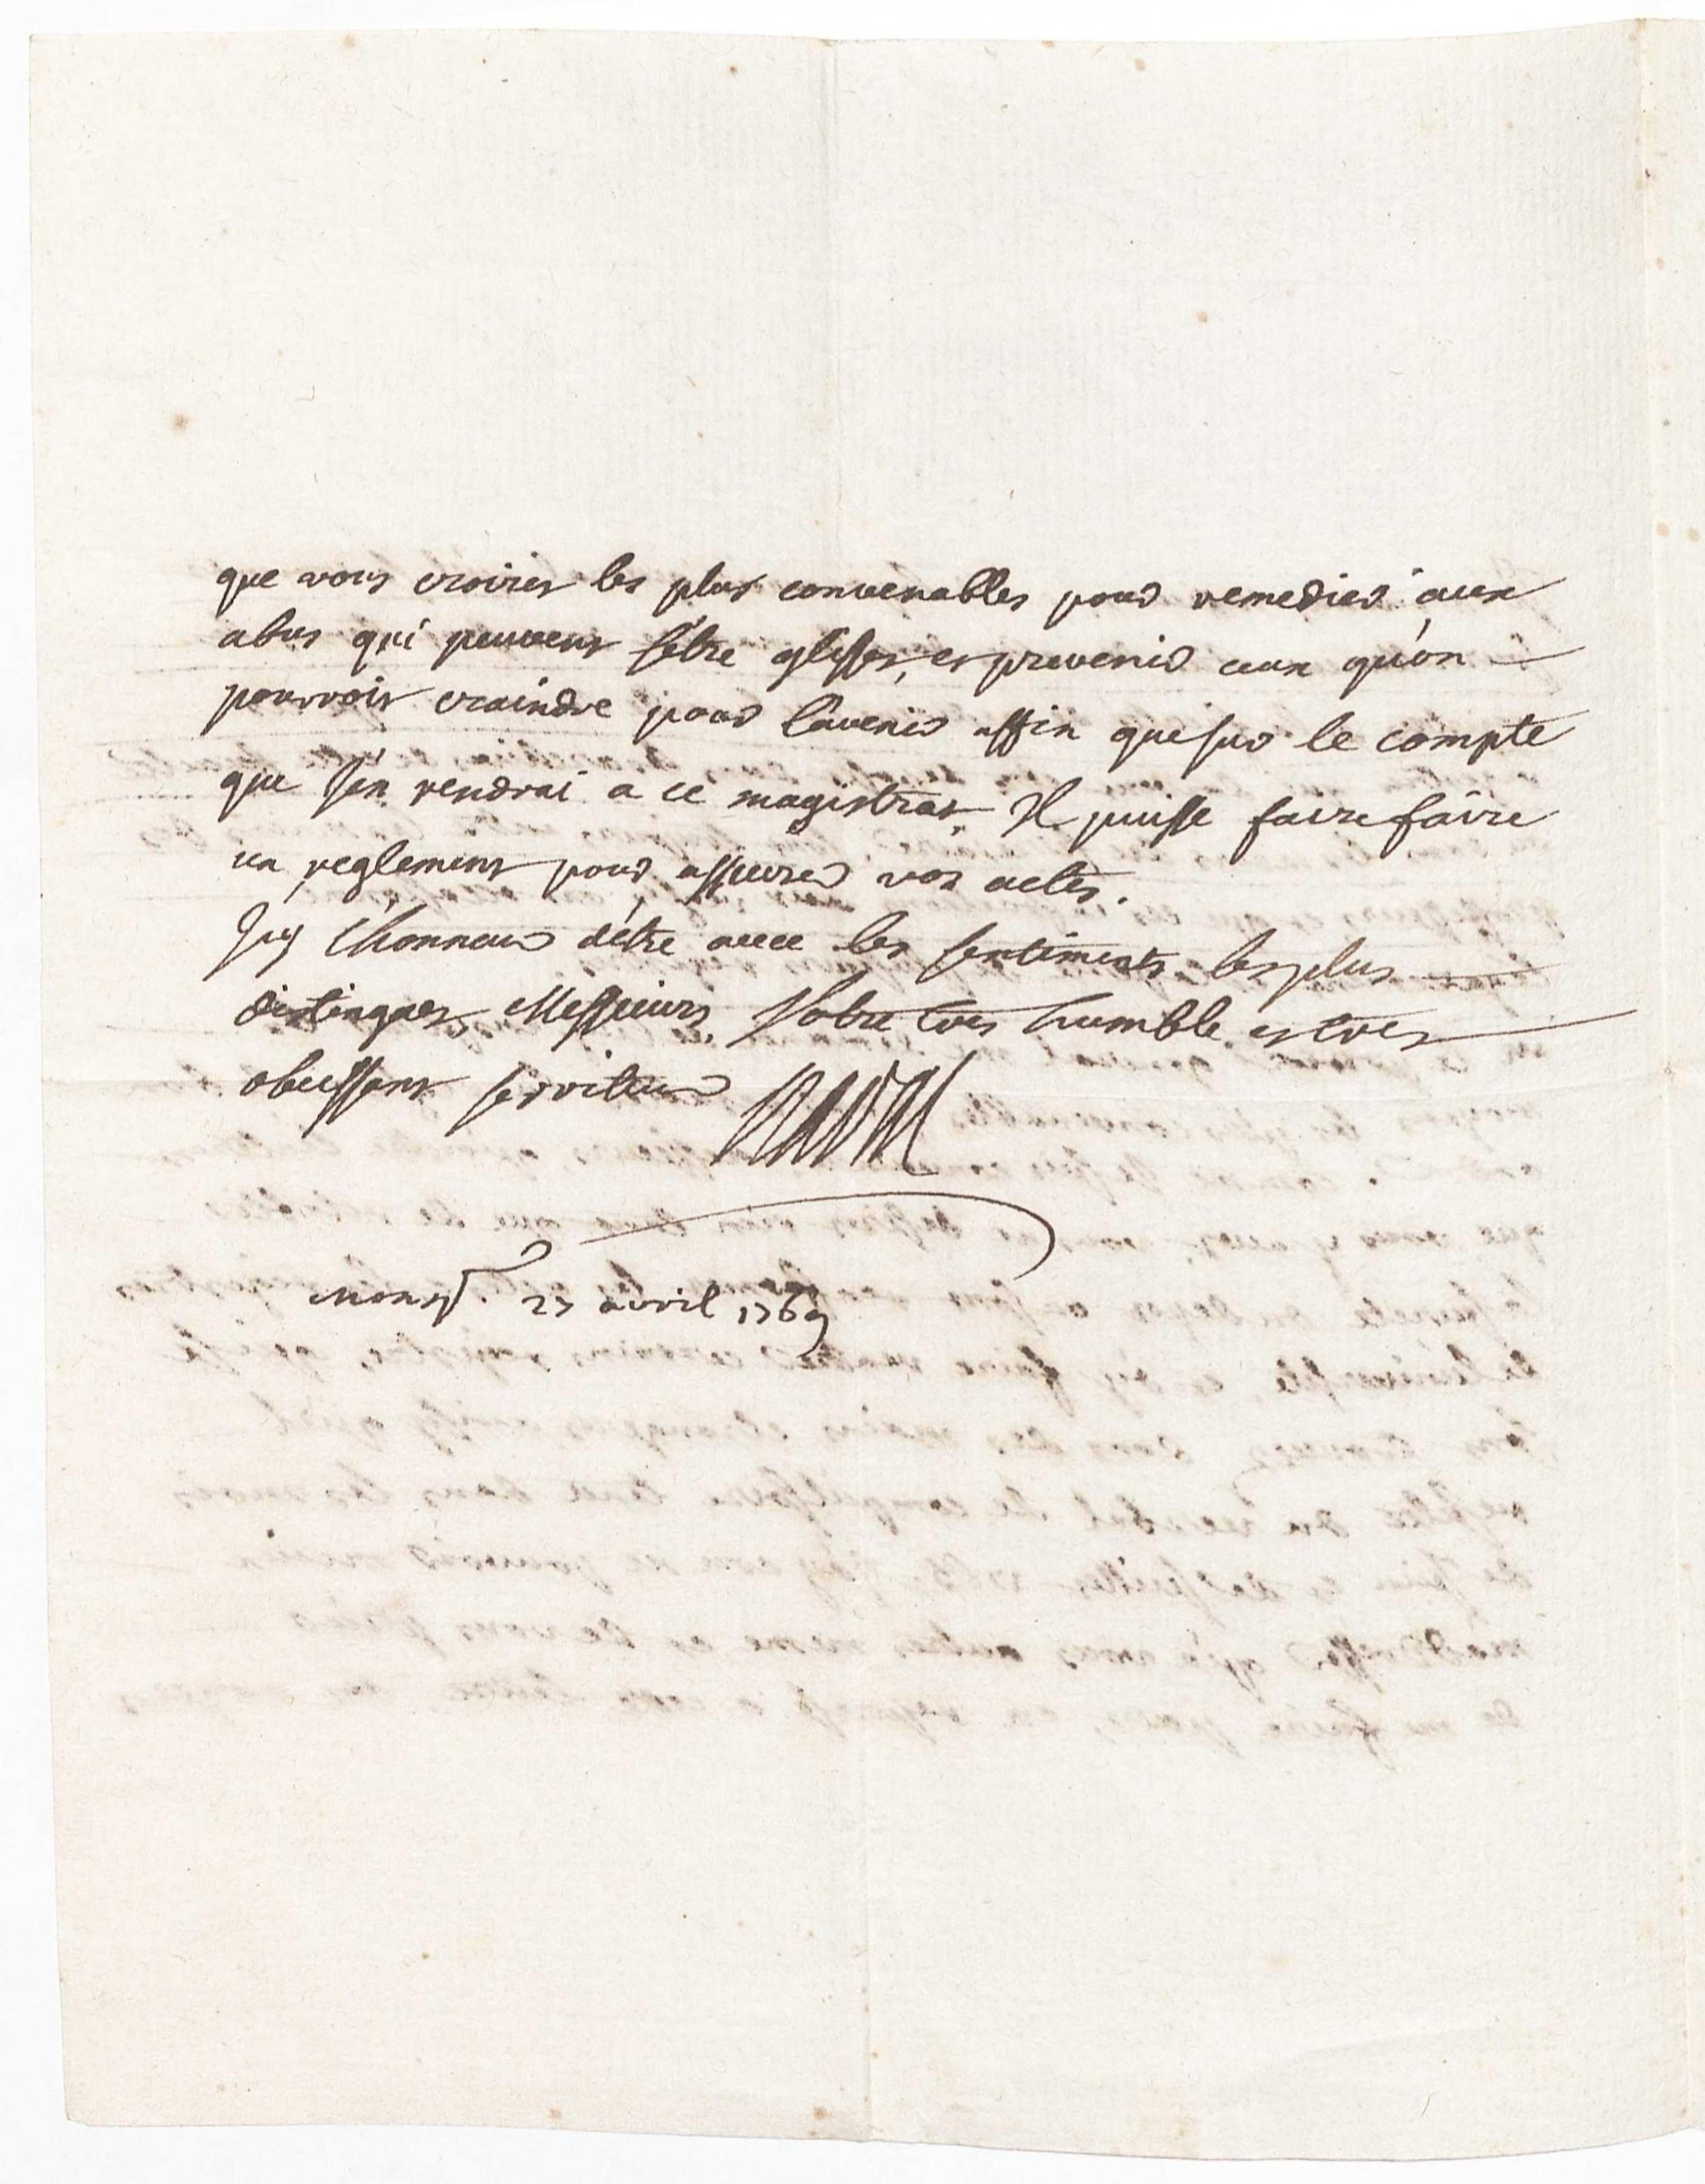
\includegraphics[
	width=\textwidth,
	height=0.78\textheight,
	keepaspectratio
	]{images/F54_20.jpg}
	\caption[Lettre relative à la mauvaise tenue des archives, seconde vue]
	{\enquote{Lettre écrite au nom du procureur général au sujet de la mauvaise tenue des archives de la Faculté et sur les mesures qu'il serait indispensable de prendre pour éviter la perte des documents}, seconde vue, 27 avril 1769, sans lieu, Montpellier, Archives historiques de la Faculté de médecine, F~54. Numérisation : Clara Martin.}
	\label{fig:f54-20}
\end{figure}

\begin{figure}[p]
	\centering
	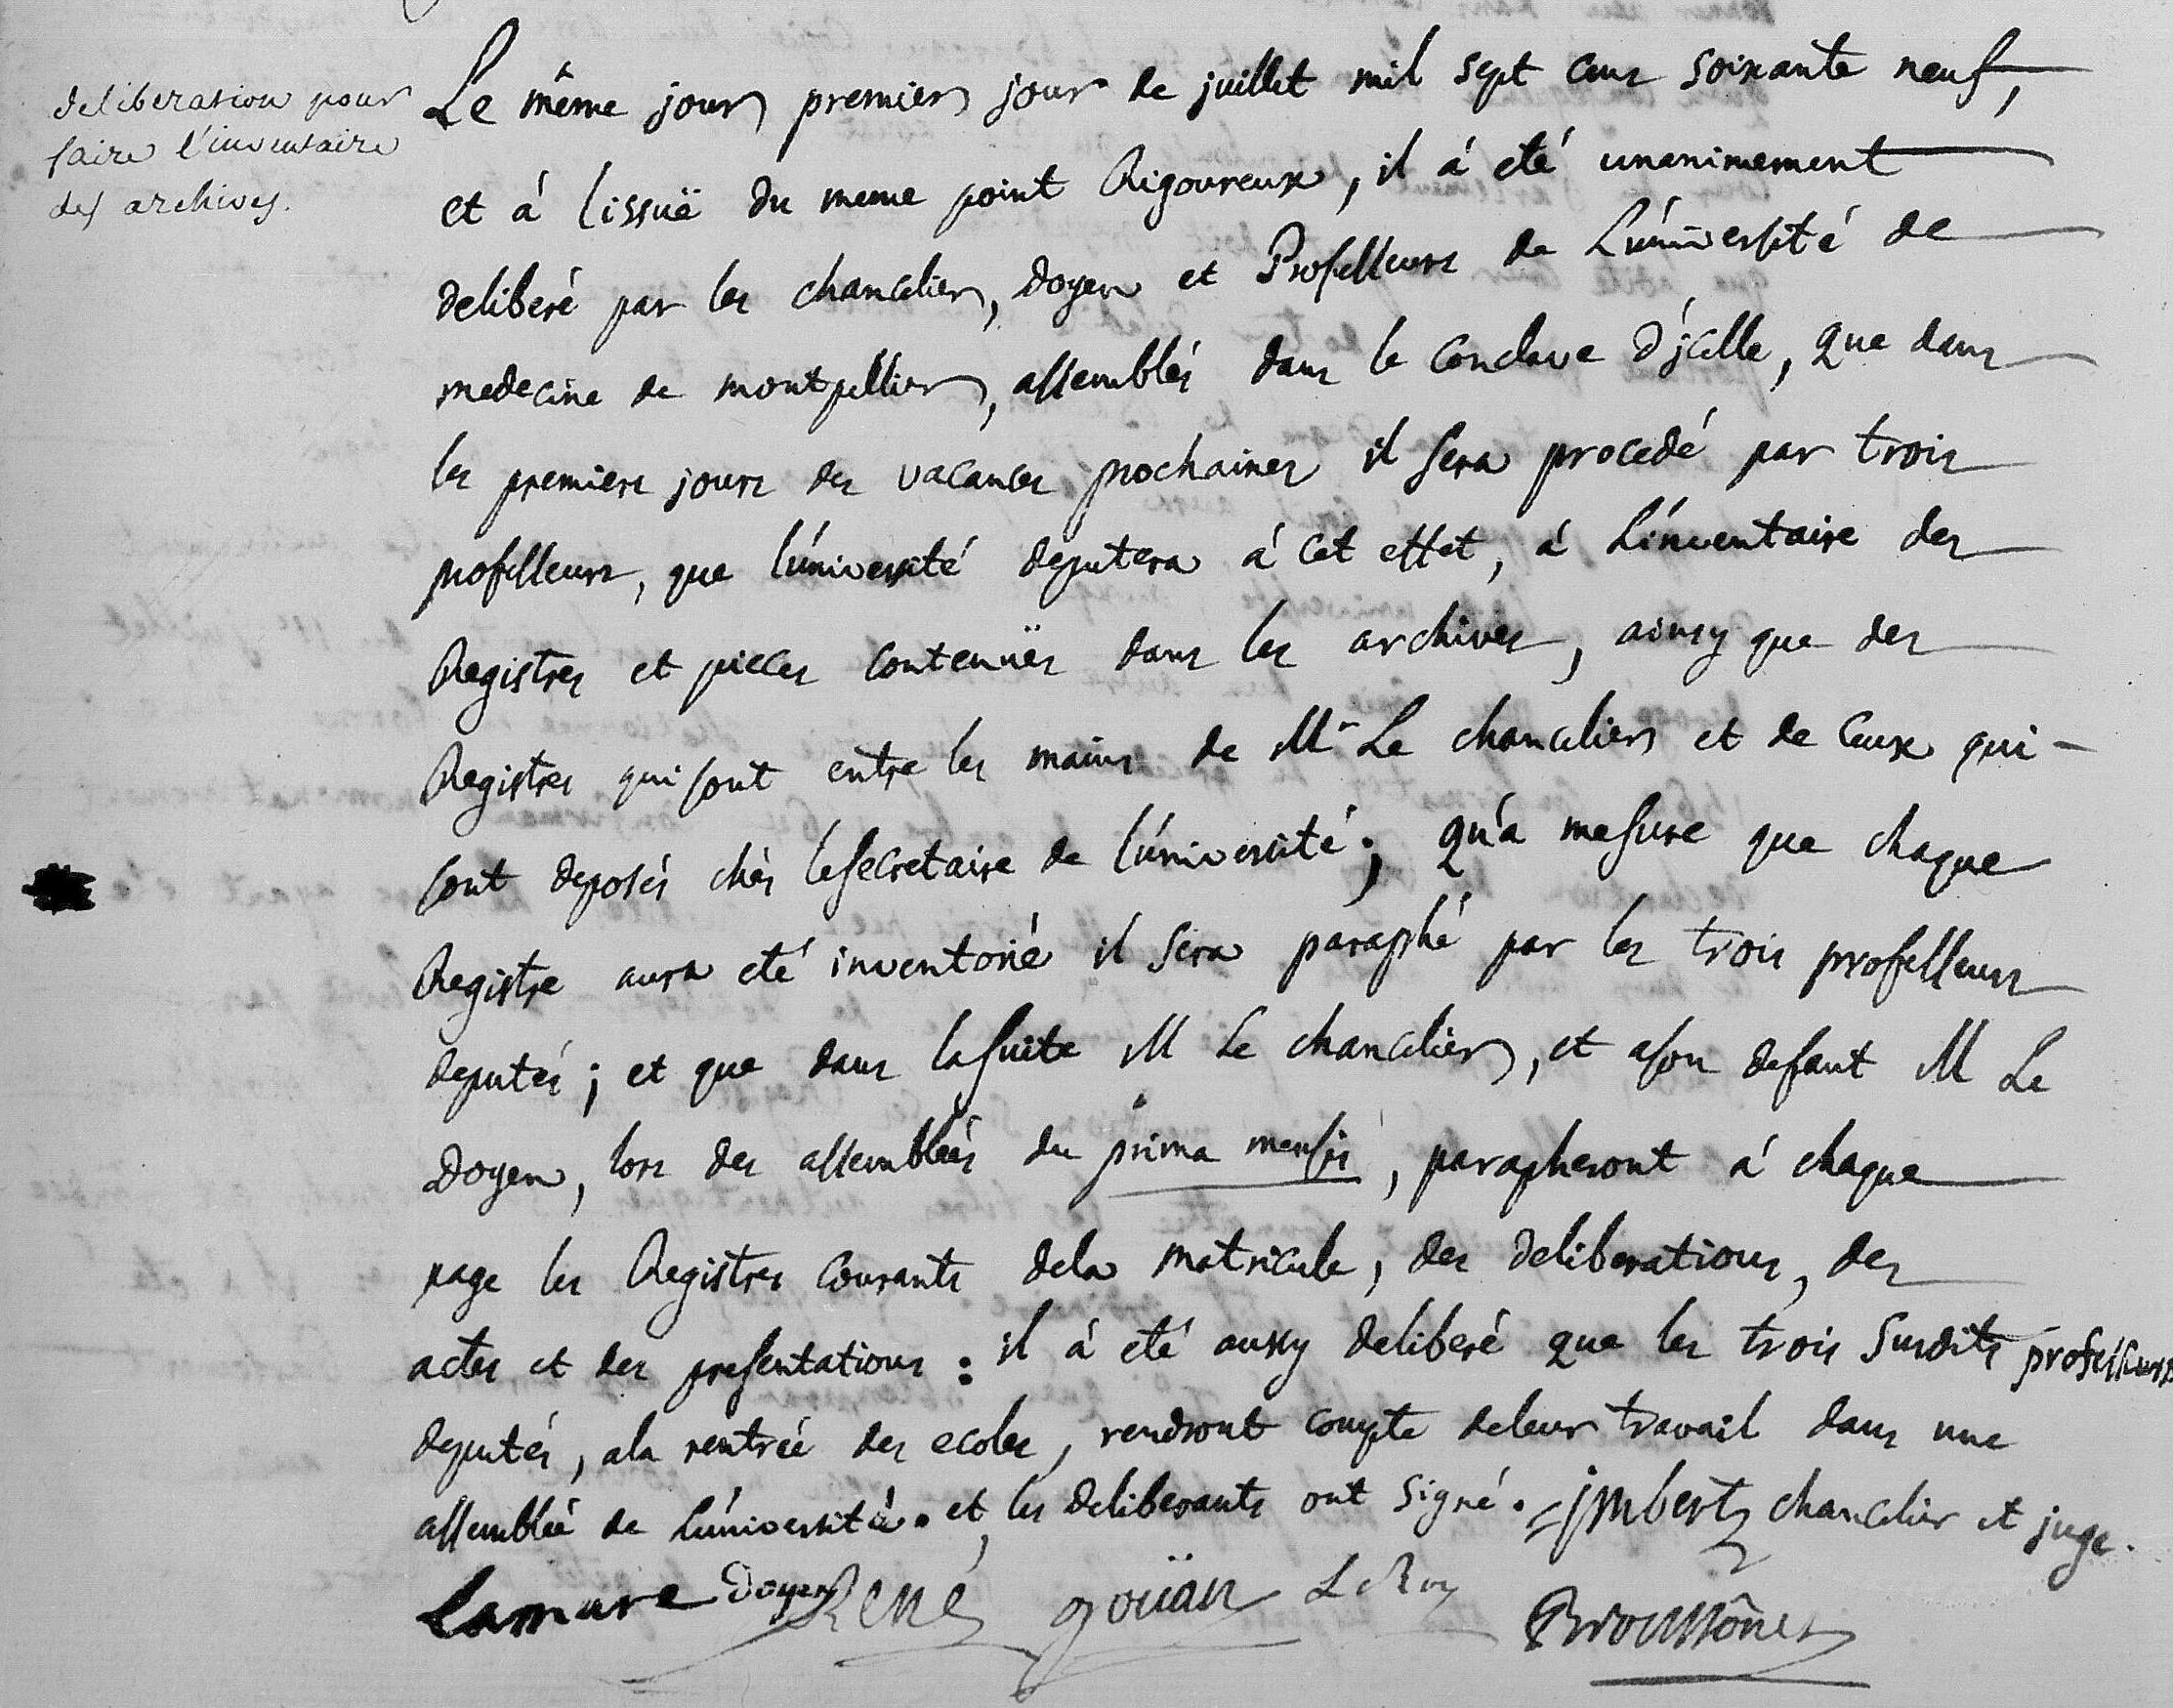
\includegraphics[
	width=\textwidth,
	height=0.78\textheight,
	keepaspectratio
	]{images/S17_p8.jpg}
	\caption[Délibération relative à la réalisation d'un nouvel inventaire, 1\textsuperscript{er} juillet 1769]
	{Délibération relative à la réalisation d'un nouvel inventaire des archives de la Faculté, 1\textsuperscript{er} juillet 1769, dans le \emph{Registre des délibérations. Suite du registre précédent} (15 octobre 1768--4 brumaire an III), Montpellier, Archives historiques de la Faculté de médecine, S~17. Numérisation : Clara Martin.}
	\label{fig:s17-p8}
\end{figure}

\begin{figure}[p]
	\centering
	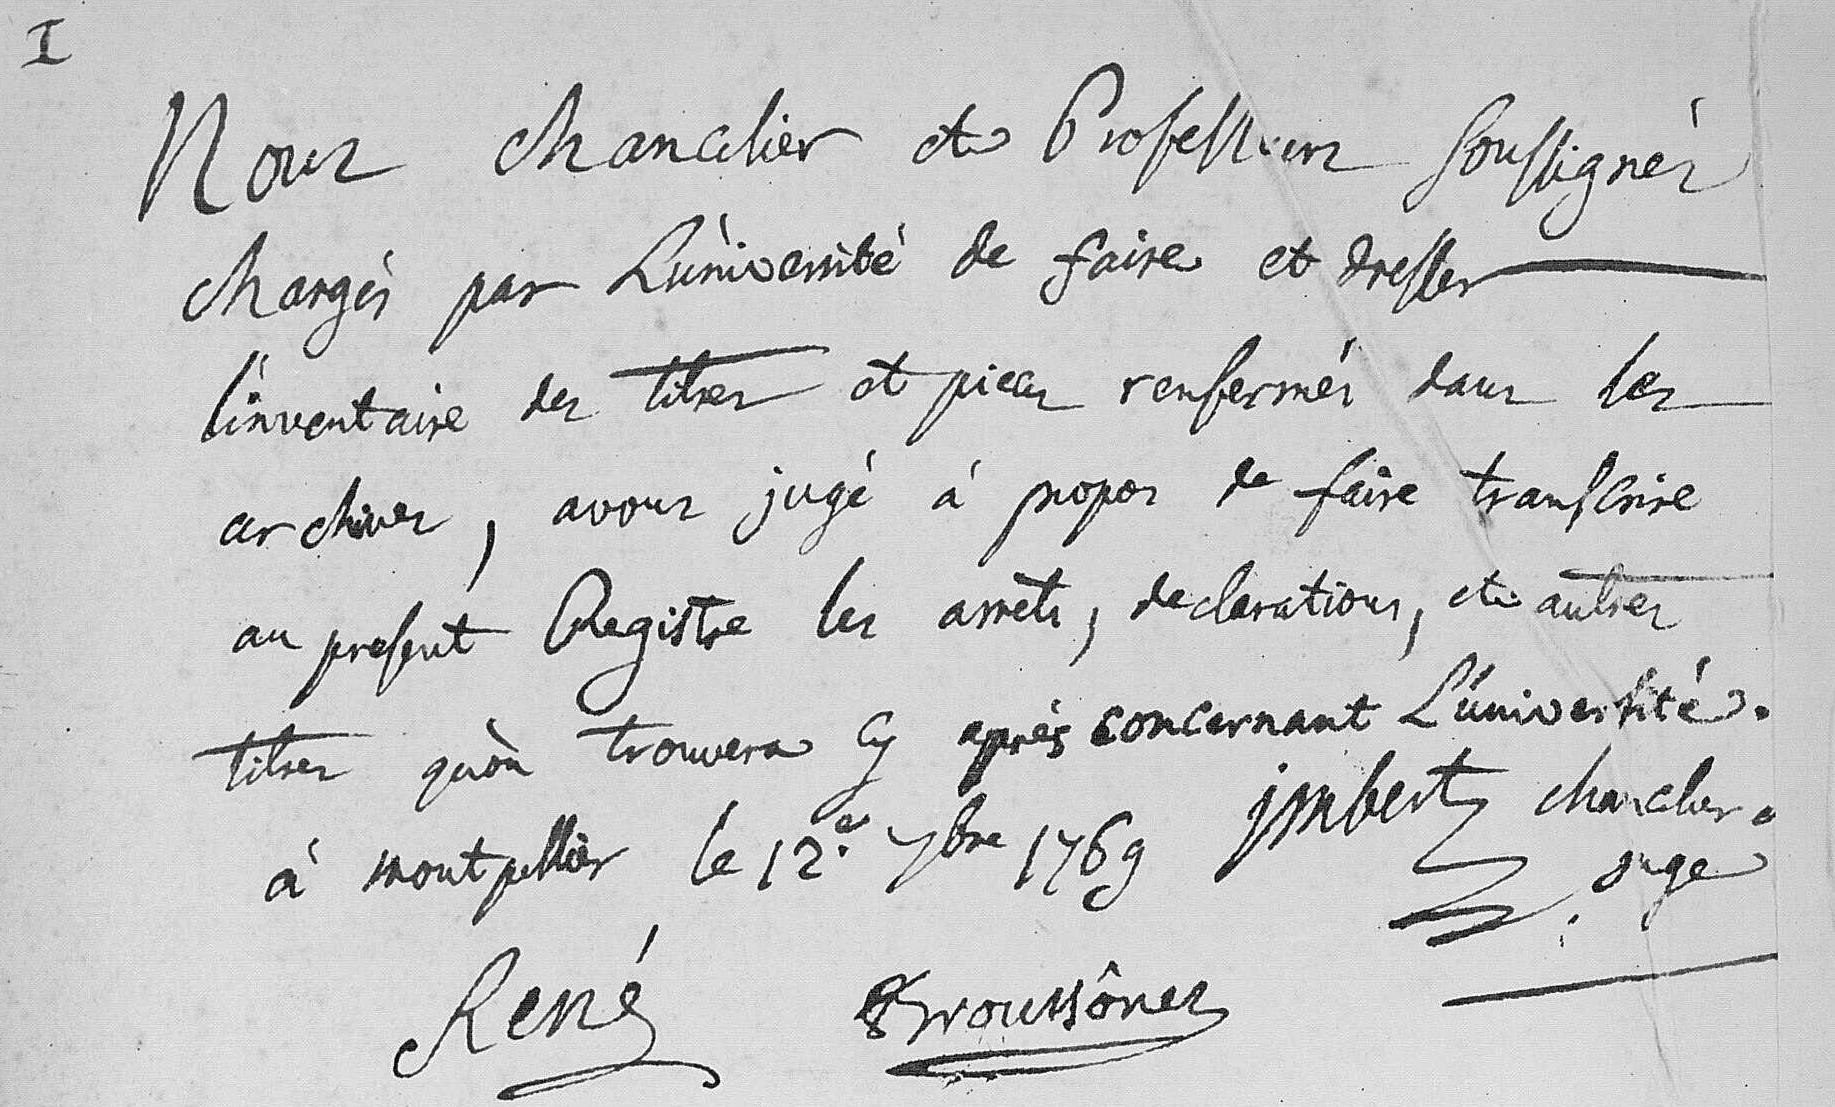
\includegraphics[
	width=\textwidth,
	height=0.78\textheight,
	keepaspectratio
	]{images/S3_f1.jpg}
	\caption[Ouverture du registre des \emph{Arrêts et Déclarations}, 12 septembre 1769]
	{Déclaration liminaire relative à la transcription des arrêts, déclarations et autres titres concernant l'Université, 12 septembre 1769, fol.~1, registre des \emph{Arrêts et Déclarations}, Montpellier, Archives historiques de la Faculté de médecine, S~3. Numérisation : Clara Martin.}
	\label{fig:s3-f1}
\end{figure}

\begin{figure}[p]
	\centering
	
	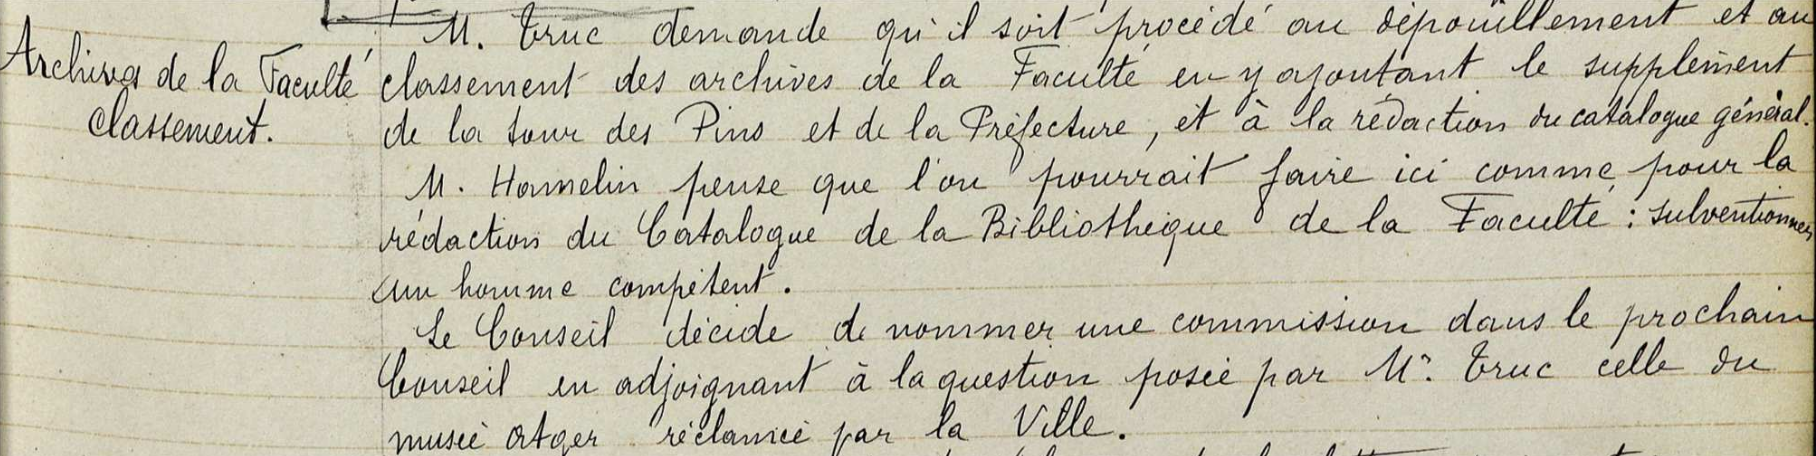
\includegraphics[
	width=\textwidth,
	height=0.30\textheight,
	keepaspectratio
	]{images/1MED51_calmette.png}
	\caption[Décision de classer les archives de la Faculté, 24 juillet 1902]
	{Délibération du conseil de faculté du 24 juillet 1902 décidant du classement des archives, Montpellier, Archives historiques de la Faculté de médecine, 1~MED~51. Numérisation : Sophie Dikoff.}
	\label{fig:1med51-calmette}
	
	\vspace{5em}
	
	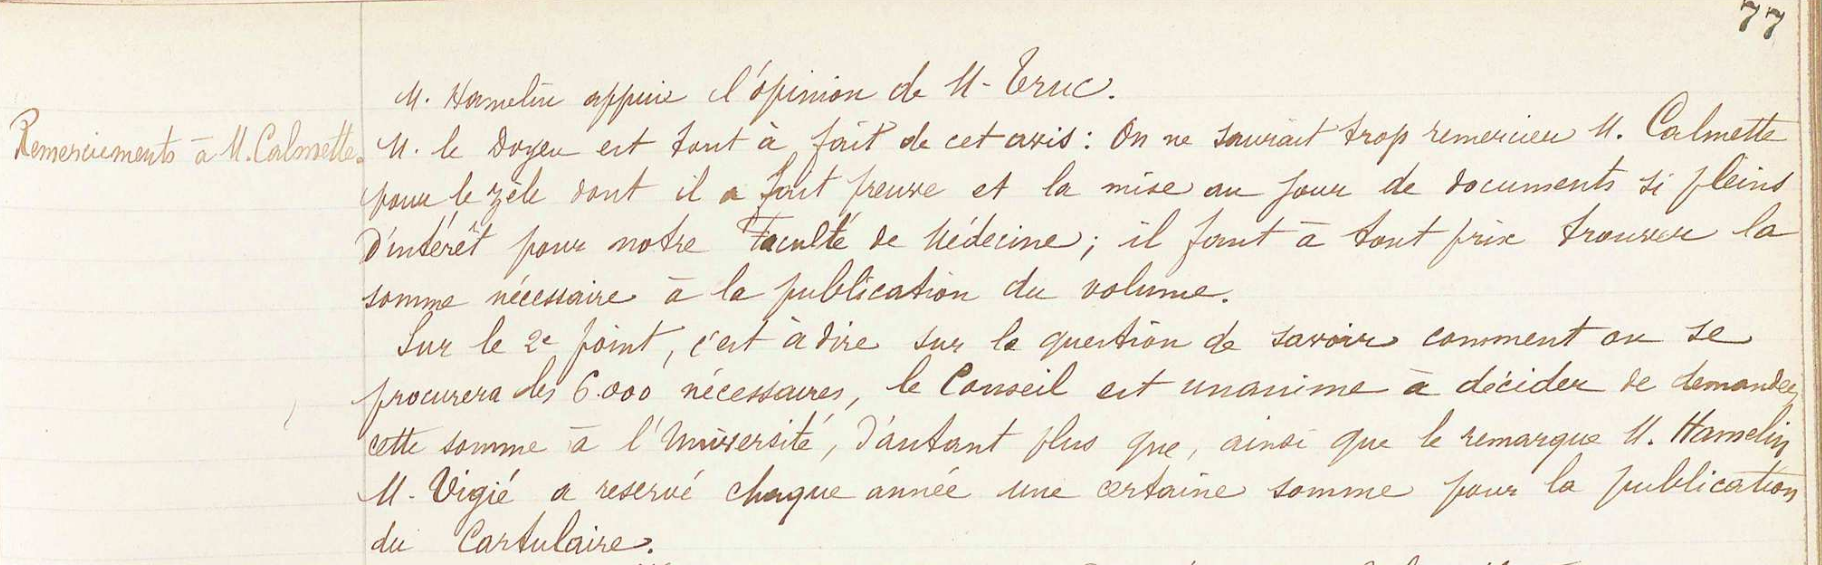
\includegraphics[
	width=\textwidth,
	height=0.30\textheight,
	keepaspectratio
	]{images/1MED52_calmette.png}
	\caption[Remerciements à Joseph Calmette et publication du \emph{Cartulaire}, 9 novembre 1907]
	{Délibération du conseil de faculté du 9 novembre 1907 remerciant Joseph Calmette et décidant de la publication du \emph{Cartulaire}, Montpellier, Archives historiques de la Faculté de médecine, 1~MED~52. Numérisation : Sophie Dikoff.}
	\label{fig:1med52-calmette}
\end{figure}

\chapter{Organisation de la Direction de la culture scientifique et du patrimoine historique}
\label{annexe:dcSPH}

\begin{landscape}
	\begin{figure}[p]
		\centering
		
		\rotatebox{180}{%
			\begin{minipage}{\linewidth}
				\centering
				
				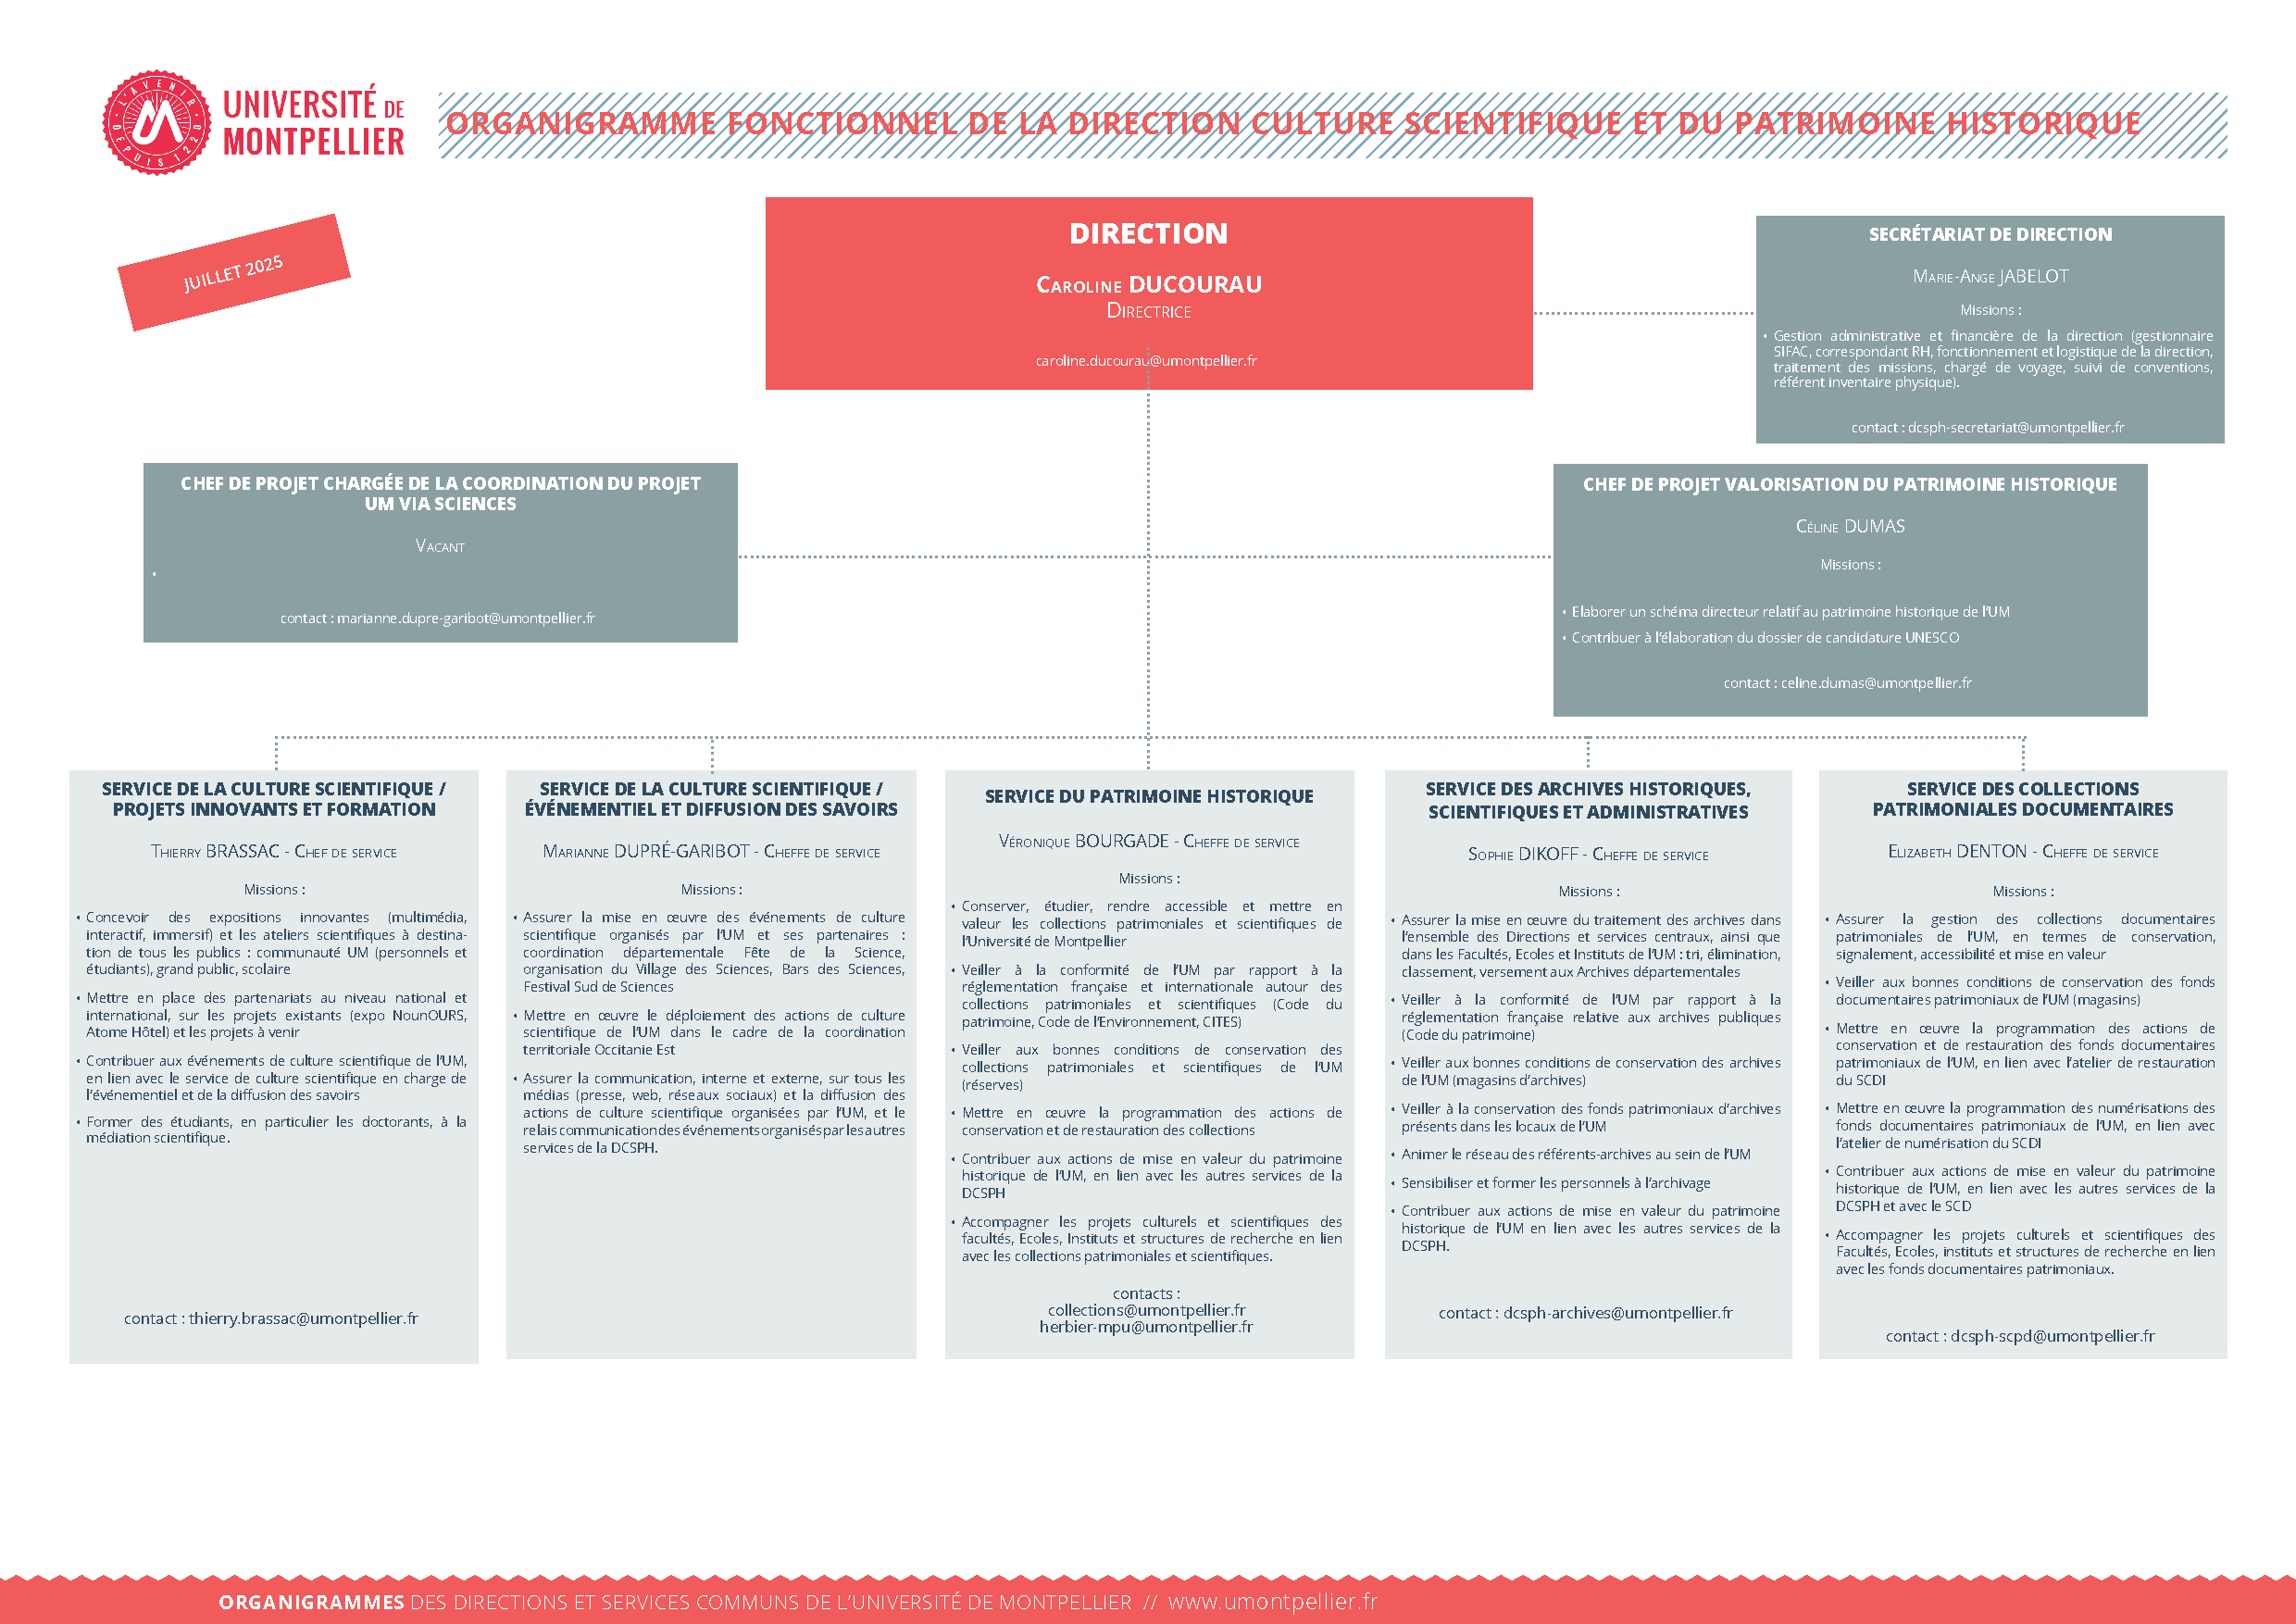
\includegraphics[
				page=1,
				width=1.08\linewidth,
				height=0.92\textheight,
				keepaspectratio
				]{images/DCSPH.pdf}
				
				\captionof{figure}
				[Organisation de la Direction de la culture scientifique et du patrimoine historique]
				{Organisation de la Direction de la culture scientifique et du patrimoine historique de l'Université de Montpellier, juillet 2025.}
				
				\label{fig:dcSPH-2025}
				
			\end{minipage}%
		}
		
	\end{figure}
\end{landscape}

	
	
	% ------------------------
	% Éléments de fin
	% ------------------------
	
	\backmatter
	\pagestyle{plain}
	
	% Liste alphabétique des sigles employés
	\printglossary[
	type=\acronymtype,
	title={Liste des sigles}
	]
	
	% Glossaire des principaux termes techniques effectivement employés
	\printglossary[
	title={Glossaire}
	]
	
	% Table des matières placée à la fin selon les modèles TNAH
	\tableofcontents
	
\end{document}